%% Beginning of file 'Optimizing_AI_Workloads_for_Enhanced_Performance__A_Comprehensive_Framework_for_Comparing_CPU_and_GPU_Architectures.tex'
%%
%% Version 7. Created January 2025.  
%%
%% AASTeX v7 calls the following external packages:
%% times, hyperref, ifthen, hyphens, longtable, xcolor, 
%% bookmarks, array, rotating, ulem, and lineno 
%%
%% RevTeX is no longer used in AASTeX v7.
%%
\documentclass[modern,longauthor]{aastex7}
\usepackage{changepage}
\usepackage{endnotes}
\let\footnote=\endnote
\usepackage{listings}
\usepackage{placeins}
\usepackage{subcaption}
%%
%% This initial command takes arguments that can be used to easily modify 
%% the output of the compiled manuscript. Any combination of arguments can be 
%% invoked like this:
%%
%% \documentclass[argument1,argument2,argument3,...]{aastex7}
%%
%% Six of the arguments are typestting options. They are:
%%
%%  twocolumn   : two text columns, 10 point font, single spaced article.
%%                This is the most compact and represent the final published
%%                derived PDF copy of the accepted manuscript from the publisher
%%  default     : one text column, 10 point font, single spaced (default).
%%  manuscript  : one text column, 12 point font, double spaced article.
%%  preprint    : one text column, 12 point font, single spaced article.  
%%  preprint2   : two text columns, 12 point font, single spaced article.
%%  modern      : a stylish, single text column, 12 point font, article with
%% 		  wider left and right margins. This uses the Daniel
%% 		  Foreman-Mackey and David Hogg design.
%%
%% Note that you can submit to the AAS Journals in any of these 6 styles.
%%
%% There are other optional arguments one can invoke to allow other stylistic
%% actions. The available options are:
%%
%%   astrosymb    : Loads Astrosymb font and define \astrocommands. 
%%   tighten      : Makes baselineskip slightly smaller, only works with 
%%                  the twocolumn substyle.
%%   times        : uses times font instead of the default.
%%   linenumbers  : turn on linenumbering. Note this is mandatory for AAS
%%                  Journal submissions and revisions.
%%   trackchanges : Shows added text in bold.
%%   longauthor   : Do not use the more compressed footnote style (default) for 
%%                  the author/collaboration/affiliations. Instead print all
%%                  affiliation information after each name. Creates a much 
%%                  longer author list but may be desirable for short 
%%                  author papers.
%% twocolappendix : make 2 column appendix.
%%   anonymous    : Do not show the authors, affiliations, acknowledgments,
%%                  and author contributions for dual anonymous review.
%%  resetfootnote : Reset footnotes to 1 in the body of the manuscript.
%%                  Useful when there are a lot of authors and affiliations
%%		    in the front matter.
%%   longbib      : Print article titles in the references. This option
%% 		    is mandatory for PSJ manuscripts.
%%
%% Since v6, AASTeX has included \hyperref support. While we have built in 
%% specific %% defaults into the classfile you can manually override them 
%% with the \hypersetup command. For example,
%%
%% \hypersetup{linkcolor=red,citecolor=green,filecolor=cyan,urlcolor=magenta}
%%
%% will change the color of the internal links to red, the links to the
%% bibliography to green, the file links to cyan, and the external links to
%% magenta. Additional information on \hyperref options can be found here:
%% https://www.tug.org/applications/hyperref/manual.html#x1-40003
%%
%% The "bookmarks" has been changed to "true" in hyperref
%% to improve the accessibility of the compiled pdf file.
%%
%% If you want to create your own macros, you can do so
%% using \newcommand. Your macros should appear before
%% the \begin{document} command.
%%
\newcommand{\vdag}{(v)^\dagger}
\newcommand\aastex{AAS\TeX}
\newcommand\latex{La\TeX}
%%%%%%%%%%%%%%%%%%%%%%%%%%%%%%%%%%%%%%%%%%%%%%%%%%%%%%%%%%%%%%%%%%%%%%%%%%%%%%%%
%%
%% The following section outlines numerous optional output that
%% can be displayed in the front matter or as running meta-data.
%%
%% Running header information. A short title on odd pages and 
%% short author list on even pages. Note that this
%% information may be modified in production.
%%\shorttitle{AASTeX v7 Sample article}
%%\shortauthors{The Terra Mater collaboration}
%%
%% Include dates for submitted, revised, and accepted.
%%\received{February 1, 2025}
%%\revised{March 1, 2025}
%%\accepted{\today}
%%
%% Indicate AAS Journal the manuscript was submitted to.
%%\submitjournal{PSJ}
%% Note that this command adds "Submitted to " the argument.
%%
%% You can add a light gray and diagonal water-mark to the first page 
%% with this command:
%% \watermark{text}
%% where "text", e.g. DRAFT, is the text to appear.  If the text is 
%% long you can control the water-mark size with:
%% \setwatermarkfontsize{dimension}
%% where dimension is any recognized LaTeX dimension, e.g. pt, in, etc.
%%%%%%%%%%%%%%%%%%%%%%%%%%%%%%%%%%%%%%%%%%%%%%%%%%%%%%%%%%%%%%%%%%%%%%%%%%%%%%%%
%%
%% Use this command to indicate a subdirectory where figures are located.
%%\graphicspath{{./}{figures/}}
%% This is the end of the preamble.  Indicate the beginning of the
%% manuscript itself with \begin{document}.
\begin{document}
\title{
Optimizing AI Workloads for Enhanced Performance: A Comprehensive Framework for Comparing CPU and GPU Architectures
\vspace{1mm}
\\\small\textnormal{In-Depth Benchmarking and Evaluation of Multithreading, OpenMP, SIMD, Quantization, Compiler Selection, and CUDA Tuning for Accelerated Machine Learning Tasks}
\vspace{1mm}
}
%% A significant change from AASTeX v6+ is in the author blocks. Now an email
%% address is required for each author. This means that each author requires
%% at least one of the following:
%%
%% \author
%% \affiliation
%% \email
%%
%% If these three commands are not available for each author, the latex
%% compiler will issue an error and if you force the latex compiler to continue,
%% it will generate an incomplete pdf.
%%
%% Multiple \affiliation commands are allowed and authors can also include
%% an optional \altaffiliation to indicate a status, i.e. Hubble Fellow. 
%% while affiliations are indexed as footnotes, altaffiliations are noted with
%% with a non-numeric footnote that is set away from the numeric \affiliation 
%% footnotes. NOTE that if an \altaffiliation command is used it must 
%% come BEFORE the \affiliation call, right after the \author command, in 
%% order to place the footnotes in the proper location. Because non-numeric
%% symbols are used, \altaffiliation should be used sparingly.
%%
%% In v7 the \author command takes an optional argument which provides 
%% additional metadata about the author. Authors can provide the 16 digit 
%% ORCID, the surname (family or last) name, the given (first or fore-) name, 
%% and a name suffix, e.g. "Jr.". The syntax is:
%%
%% \author[orcid=0000-0002-9072-1121,gname=Gregory,sname=Schwarz]{Greg Schwarz}
%%
%% This name metadata in not shown, it is only for parsing by the peer review
%% system so authors can be more easily identified. This name information will
%% also be sent to the publisher so they can include it in the CROSSREF 
%% metadata. Including an orcid will hyperlink the author name to the 
%% author's ORCID page. Note that  during compilation, LaTeX will do some 
%% limited checking of the format of the ID to make sure it is valid. If 
%% the "orcid-ID.png" image file is  present or in the LaTeX pathway, the 
%% ORCID icon will appear next to the authors name.
%%
%% Even though emails are now required for each author, the \email does not
%% produce output in the compiled manuscript unless the optional "show" command
%% is used. For example,
%%
%% \email[show]{greg.schwarz@aas.org}
%%
%% All "shown" emails are show in the bottom left of the first page. Due to
%% space constraints, only a few emails should be shown. 
%%
%% To identify a corresponding author, use the \correspondingauthor command.
%% The command appends "Corresponding Author: " to the argument it appears at
%% the bottom left of the first page like the output from \email. 
\author[]{Maximilian Achenbach}
\affiliation{Friedrich-Alexander-University Erlangen-Nuremberg}
\affiliation{Matriculation number: 22988102}
\affiliation{Email: max.achenbach@fau.de}
\email[]{max.achenbach@fau.de}

\author[]{Dustin Heither} 
\affiliation{Friedrich-Alexander-University Erlangen-Nuremberg}
\affiliation{Matriculation number: 23004228}
\affiliation{Email: dustin.heither@fau.de}
\email[]{dustin.heither@fau.de}

\author[]{Robert Kagan}
\affiliation{Friedrich-Alexander-University Erlangen-Nuremberg}
\affiliation{Matriculation number: 22965026}
\affiliation{Email: robert.kagan@fau.de}
\email[]{robert.kagan@fau.de}
%% Use the \collaboration command to identify collaborations. This command
%% takes an optional argument that is either a number or the word "all"
%% which tells the compiler how many of the authors above the command to
%% show. For example "\collaboration[all]{(DELVE Collaboration)}" wil include
%% all the authors above this command.
%%
%% Mark off the abstract in the ``abstract'' environment. 
\begin{abstract}
This project presents a unified framework for artificial intelligence (AI) applications, optimized for both CPU and GPU architectures, to systematically investigate performance trade-offs across hardware platforms. Using the MNIST dataset as a foundational benchmark, the study examines computational efficiency and scalability to problem size. A comprehensive suite of optimization strategies—including multithreading, OpenMP, SIMD, quantization, compiler selection, CUDA tuning, memory management, and thread-level parallelism—is implemented and analyzed to assess their impact on runtime and resource utilization.

Experimental results show that GPU-based optimizations reduce runtime by up to 73.6\% on large-scale workloads, while CPU optimizations achieve runtime reductions of up to 90.4\% on the synthetic XL dataset. In the final comparison, GPUs prove to be 52.3\% slower than CPUs for small problem sizes; however, as the problem size increases, this trend reverses, with GPUs demonstrating a 17.7\% performance advantage over CPUs. Moreover, advances in CPU architecture—such as Apple Silicon—deliver notable performance gains, outperforming even GPUs and underscoring the significance of generational hardware improvements.

The findings highlight the effectiveness of diverse optimization strategies, clarify the strengths and limitations of heterogeneous computing resources, and offer practical guidance for adaptive AI deployment. By emphasizing reproducibility and extensibility, this work establishes a solid foundation for future research on more complex datasets and advanced AI workloads.
\end{abstract}
%% Keywords should appear after the \end{abstract} command. 
%% The AAS Journals now uses Unified Astronomy Thesaurus (UAT) concepts:
%% https://astrothesaurus.org
%% You will be asked to selected these concepts during the submission process
%% but this old "keyword" functionality is maintained in case authors want
%% to include these concepts in their preprints.
%%
%% You can use the \uat command to link your UAT concepts back its source.
%% \keywords{\uat{Galaxies}{573} --- \uat{Cosmology}{343} --- \uat{High Energy astrophysics}{739} --- \uat{Interstellar medium}{847} --- \uat{Stellar astronomy}{1583} --- \uat{Solar physics}{1476}}
%% From the front matter, we move on to the body of the paper.
%% Sections are demarcated by \section and \subsection, respectively.
%% Observe the use of the LaTeX \label
%% command after the \subsection to give a symbolic KEY to the
%% subsection for cross-referencing in a \ref command.
%% You can use LaTeX's \ref and \label commands to keep track of
%% cross-references to sections, equations, tables, and figures.
%% That way, if you change the order of any elements, LaTeX will
%% automatically renumber them.
\section{Introduction}\label{sec:introduction}
We are entering the age of artificial intelligence (AI). While deep learning was once considered a niche area of research, it has rapidly evolved into a foundational component of modern software and services. Its influence now spans a wide range of applications, including personalized recommendations, voice assistants, AI agents, real-time language translation, and medical diagnostics. At the computational core of these systems lie neural networks, which enable models to learn complex patterns from data and generalize across diverse tasks.

As neural networks increase in complexity and capability, so too do the demands placed on computing infrastructure. Large-scale models now comprise billions of parameters, require massive datasets, and rely on increasingly specialized hardware to deliver competitive performance. However, beyond the training phase, efficient inference—the ability to execute models quickly, reliably, and with minimal energy consumption—has become equally critical. This is particularly relevant in latency-sensitive scenarios such as autonomous vehicles, or in resource-constrained environments like smartphones and embedded systems.

This ongoing shift has elevated the computation of deep learning algorithms, particularly neural networks, from a subfield of machine learning to a central concern in systems engineering. Throughput, memory efficiency, parallelism, and hardware compatibility are no longer secondary considerations—they must be addressed from the outset to ensure robust and scalable deployment of real-world AI applications. As artificial intelligence continues to integrate more deeply into everyday life, optimizing the performance of deep learning systems has become essential to ensuring their scalability, accessibility, and long-term sustainability.
\section{Objective}\label{sec:objective}
In this project, we are focused on developing a unified framework for artificial intelligence applications that supports both CPUs and GPUs. Our primary objective is to explore and compare the advantages and disadvantages of these two hardware architectures. To achieve this, we will utilize a wide and representative range of hardware systems, along with a set of self-developed and carefully evaluated benchmarks that reflect real-world application scenarios. These benchmarks will provide valuable insights into the performance differences between CPUs and GPUs in a variety of settings.

In addition to comparing the hardware architectures, our goal is to implement and study a variety of optimizations to assess their impact on performance, specifically with respect to different problem sizes. Through this process, we aim to understand which optimizations lead to significant improvements and which ones may have minimal or even negative effects on performance. Furthermore, we will explore the extent to which performance improvements are possible before reaching the limits imposed by the hardware itself.

The optimizations we plan to explore include techniques such as multithreading, OpenMP (Open Multi-Processing), SIMD (Single Instruction, Multiple Data), quantization, compiler selection, and CUDA tuning. However, this list is not exhaustive; additional optimizations may be implemented if bottlenecks are identified during the debugging and testing phases of development. Throughout the entire project, we will continuously benchmark and evaluate the performance of the system, comparing new results with previous benchmarks in order to validate or challenge our hypotheses.

At the conclusion of the project, we aim to produce a highly optimized framework that can serve as a robust and flexible tool for AI applications. This framework will be designed in such a way that it can be used, modified, and further developed by others in the future. To demonstrate the functionality of our project, we will implement a real-world, working machine learning model that is both functional and verifiable. This model will serve as a proof of concept, showcasing the practical applicability and effectiveness of the framework we develop.
\section{Benchmarking Setup}\label{sec:benchmarking-setup}
\subsection{Experimental Setup and Benchmarking Methodology}
To obtain meaningful and reliable results, a broad spectrum of currently deployed hardware is considered. On the graphics hardware side, tests are conducted using both laptop and desktop NVIDIA graphics cards. Regarding CPU hardware, in addition to desktop (AMD) and laptop (Intel) processors, Arm-based Apple Silicon processors are also included, particularly since the launch of Apple Silicon as a relevant comparison.

The benchmarks are performed after a system restart, minimizing interfering processes initiated by the operating system as much as possible without affecting the general usability of the system. These measures ensure the most precise and isolated measurement of the performance of the respective components.

In the analysis, the release years and power consumption of the tested components are also considered, with a focus on the number of threads and the total processing time. The latter includes the total time, including memory allocation. To minimize the impact of random fluctuations and initial warm-up periods, a total of twelve measurements are recorded per test run. The first two measurements are discarded, and the arithmetic mean is calculated from the remaining ten runs. Additionally, the minimum and maximum values of each measurement are reported to illustrate the variability of the results.
In addition to the standard benchmark using an MNIST image with dimensions $(30 \times 30)^2$, synthetic benchmarks with larger datasets are also conducted: XL $(32 \times 30)^2$ and XXL $(64 \times 30)^2$. These synthetic benchmarks serve to examine the long-term behavior of optimization strategies under different loads and dataset sizes.

In addition to functional testing, selected test cases also evaluate power consumption. On Apple Silicon hardware, this is conducted using the built-in tool powermetrics. The reported values represent the average derived from multiple measurements. Memory usage is assessed with valgrind. However, SIMD instructions must be disabled for this analysis, as they are classified as illegal instructions.
\subsection{Hardware Configuration}
The following tables provide an overview of the hardware utilized for benchmarking and identifying optimization steps. Table~\ref{tab:cpu} presents detailed specifications of the CPU hardware, while Table~\ref{tab:gpu} outlines the GPU hardware.
\begin{table}[htb!]
\centering
\caption{CPU Overview\label{tab:cpu}}
\begin{tabular}{p{5cm} p{2.5cm} p{2cm} p{2cm} p{2cm}}
\hline
CPU & Release Date & TDP (W) & Cores & Threads \\
\hline
AMD Ryzen 7 3800XT\footnote{AMD Ryzen 7 3800XT: \url{https://www.amd.com/en/support/downloads/drivers.html/processors/ryzen/ryzen-3000-series/amd-ryzen-7-3800xt.html} (accessed April 18, 2025).} & 07.07.2020 & 105 & 8 & 16 \\
Apple M3 Pro 11-Core\footnote{Apple M3 Pro 11-Core: \url{https://www.notebookcheck.net/Apple-M3-Pro-11-Core-Processor-Benchmarks-and-Specs.783008.0.html} (accessed April 18, 2025).} & 30.10.2023 & 27 & 5 & 11 \\
Intel Core i7-1065G7\footnote{Intel Core i7-1065G7: \url{https://www.intel.com/content/www/us/en/products/sku/196597/intel-core-i71065g7-processor-8m-cache-up-to-3-90-ghz/specifications.html} (accessed April 18, 2025).} & 01.06.2019 & 15 & 4 & 8 \\
\hline
\end{tabular}
\end{table}
\begin{table}[htb!]
\centering
\caption{GPU Overview\label{tab:gpu}}
\begin{tabular}{p{5cm} p{2.5cm} p{2cm} p{2cm} p{2cm}}
\hline
GPU & Release Date & TDP (W) & CUDA Cores & Base Clock (MHz) \\
\hline
NVIDIA GeForce RTX 2080\footnote{NVIDIA GeForce RTX 2080: \url{https://www.nvidia.com/en-us/geforce/graphics-cards/compare/} (accessed April 18, 2025).} & 20.10.2018 & 215 & 2944 & 1515 \\
NVIDIA GeForce MX350\footnote{NVIDIA GeForce MX350: \url{https://www.nvidia.com/en-us/geforce/gaming-laptops/mx-350/} (accessed April 18, 2025).} & 01.02.2020 & 20 & 640 & 1354 \\
\hline
\end{tabular}
\end{table}
\section{Naive Implementation}\label{sec:naive-implementation}
\subsection{Preparations}
Before implementing our own framework for artificial intelligence applications, we first need to determine its core functions and select an example that effectively demonstrates its functionality. Since our project is specifically intended to facilitate the inference of a pre-trained model, we must acquire a model that is already trained, along with its corresponding input data and weights, all in a format that is easy to integrate into our future framework.  

To meet these requirements, we decide to use an existing dataset, problem, and framework to handle the training process. Our main goal in this phase is to identify the necessary functions for our framework and ensure that we can reuse the exported input data and weights. After considering various options, we choose the well-known MNIST dataset, which contains images of handwritten digits. This dataset is widely used in machine learning and serves as a small-scale, well-understood example that allows us to focus on building and testing our framework rather than grappling with the complexity of a more intricate dataset.  

The AI model's task is to recognize the digit in each image—an image classification problem that serves as an ideal starting point. For the training framework, we select TensorFlow v1, a highly regarded and well-documented library widely used in real-world machine learning applications. We specifically choose version 1, as it provides functions that we believe will be more easily replicable and manageable for our needs. We implement the training process in Python, the recommended programming language for TensorFlow. Once the model is trained, we identify ten key functions that will be essential for our framework, including add, biasing, 2D convolution, flatten, flip kernels, hyperbolic tangent, matrix multiplication, maxpool, ReLU, and transpose. These functions are crucial for building and executing the neural network, forming the foundation of our framework.  

For exporting the trained model's weights, we consider several options and ultimately rule out the Open Neural Network Exchange (ONNX) format.\footnote{Open Neural Network Exchange: \url{https://onnx.ai/} (accessed April 17, 2025)} To implement as much as possible from scratch, we opt for a simpler approach: a human-readable text format. This format includes a line for the x-dimension, a line for the y-dimension, a blank line, and then the matrix itself, with elements separated by spaces and line breaks. By following this approach, we ensure a clear understanding of our framework’s necessary components and establish a practical example to guide its implementation and testing.
\subsection{Naive Approach}
From the very beginning, we aim to develop the framework as well-structured and modular as possible. This means that all functionalities will be divided into logical modules, which are further separated into well-documented header files and their corresponding source code files. Each header file is enclosed with header guards to prevent multiple definitions. Initially, we will need the following five modules: matrix, input/output, tensorflow, timer, and main. We will start by writing these modules in the c programming language.

First, we implement the matrix module. In this module, we define the struct named matrix, which consists of an integer for the x-dimension, an integer for the y-dimension, and a pointer for the array itself. To create a matrix, we have written the function malloc\_matrix. It expects the x- and y-dimensions as parameters and returns a properly allocated and initialized object. If a 3-dimensional matrix is required, the function malloc\_matrix\_ptr can be used. This function additionally expects the z-dimension as a parameter and internally calls malloc\_matrix. To free the memory, we provide free\_matrix and free\_matrix\_ptr, which both accept a correctly initialized matrix as input. For debugging purposes, print\_matrix is available. It prints the matrix content in a human-readable format to stdout, with elements separated by spaces and line breaks.

Next, we implement the input/output module. In this module, the struct io is defined, where all weights and the number of images and masks exported from Python are stored. To read the data, we need two helper functions: io\_to\_matrix and get\_value. io\_to\_matrix receives a file path as input, reads the dimensions and contents of the matrix, and returns a valid matrix struct. get\_value is used to read single-line text files, where the number of images or the number of masks is stored, and it returns the integer value. These two functions are then used internally in the malloc\_io function, which creates, populates, and returns the entire struct. To release the memory allocated on the heap, free\_io can be used. The paths to the text files are stored as defines that can be modified by the compiler.

In the tensorflow module, ten functions are naively implemented: add, biasing, conv2d, flatten, flip\_kernels, hyperbolic\_tangent, matmul, maxpool, relu, and transpose. Each of these functions accepts two matrices as inputs and returns a result matrix. "Naive" in this case means that the functions are implemented without any optimizations. The code is highly inefficient but remains clear and easy to understand.

In the timer module, a timer can be started with start\_timer, stopped with stop\_timer, and the time difference between two timers can be obtained using delta\_time\_us for microseconds or delta\_time\_s for seconds. Finally, in the main module, all the modules are brought together. First, a timer is started. Then, all weights are read using malloc\_io. Next, for each image, the graph shown in Figure~\ref{fig:graph} is executed using our tensorflow functions. Afterward, all resources are freed, the timer is stopped, and the performance is written to a CSV file.
\begin{figure}[htb!]
    \centering
    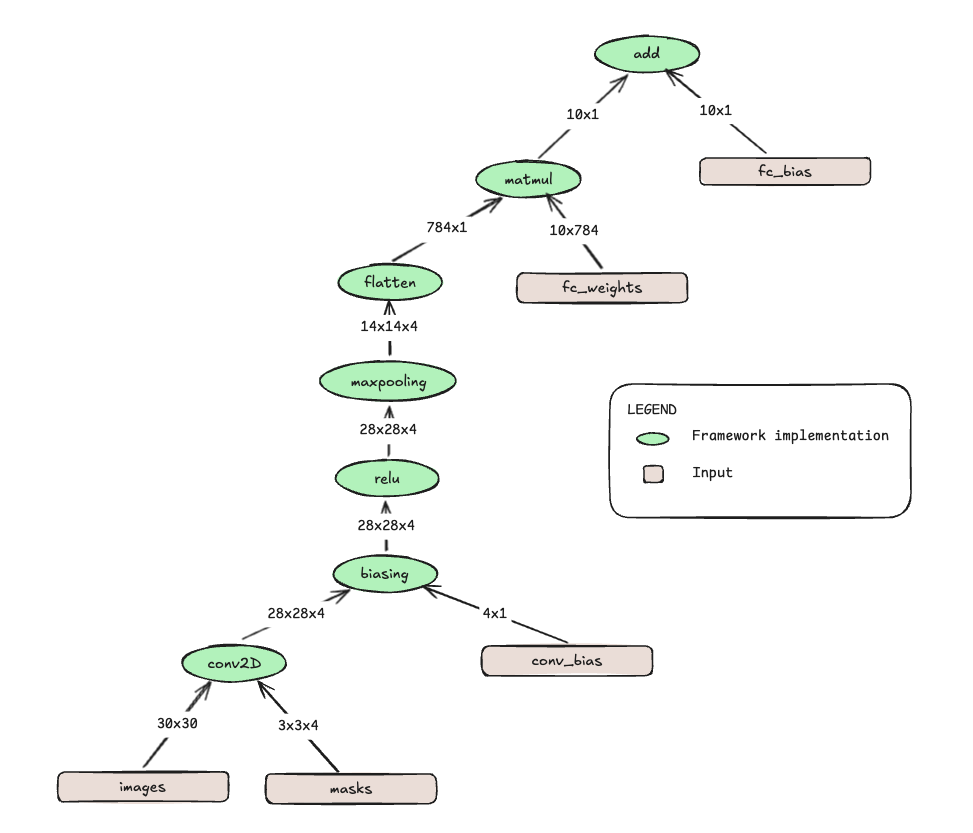
\includegraphics[width=\linewidth]{Naive/Graph.png}
    \caption{Neural network computation graph with layers and input dependencies}
   \label{fig:graph}
\end{figure}
\subsection{Performance Benchmarks}
The benchmark results are shown in Figure~\ref{fig:naive}, with the corresponding values listed in Table~\ref{tab:naive}. On the MNIST dataset, the Intel Core i7-1065G7 shows an average performance decrease of 11.6\% compared to the AMD Ryzen 7 3800XT, which itself exhibits a 42.0\% decrease relative to the Apple M3 Pro 11-Core processor. On the synthetic XL dataset, the Intel Core i7-1065G7 performs 8.3\% worse than the AMD Ryzen 7 3800XT, which in turn shows a 70.9\% performance drop compared to the Apple M3 Pro 11-Core.
\begin{figure}[htb!]
\centering
\begin{subfigure}{.5\textwidth}
  \centering
  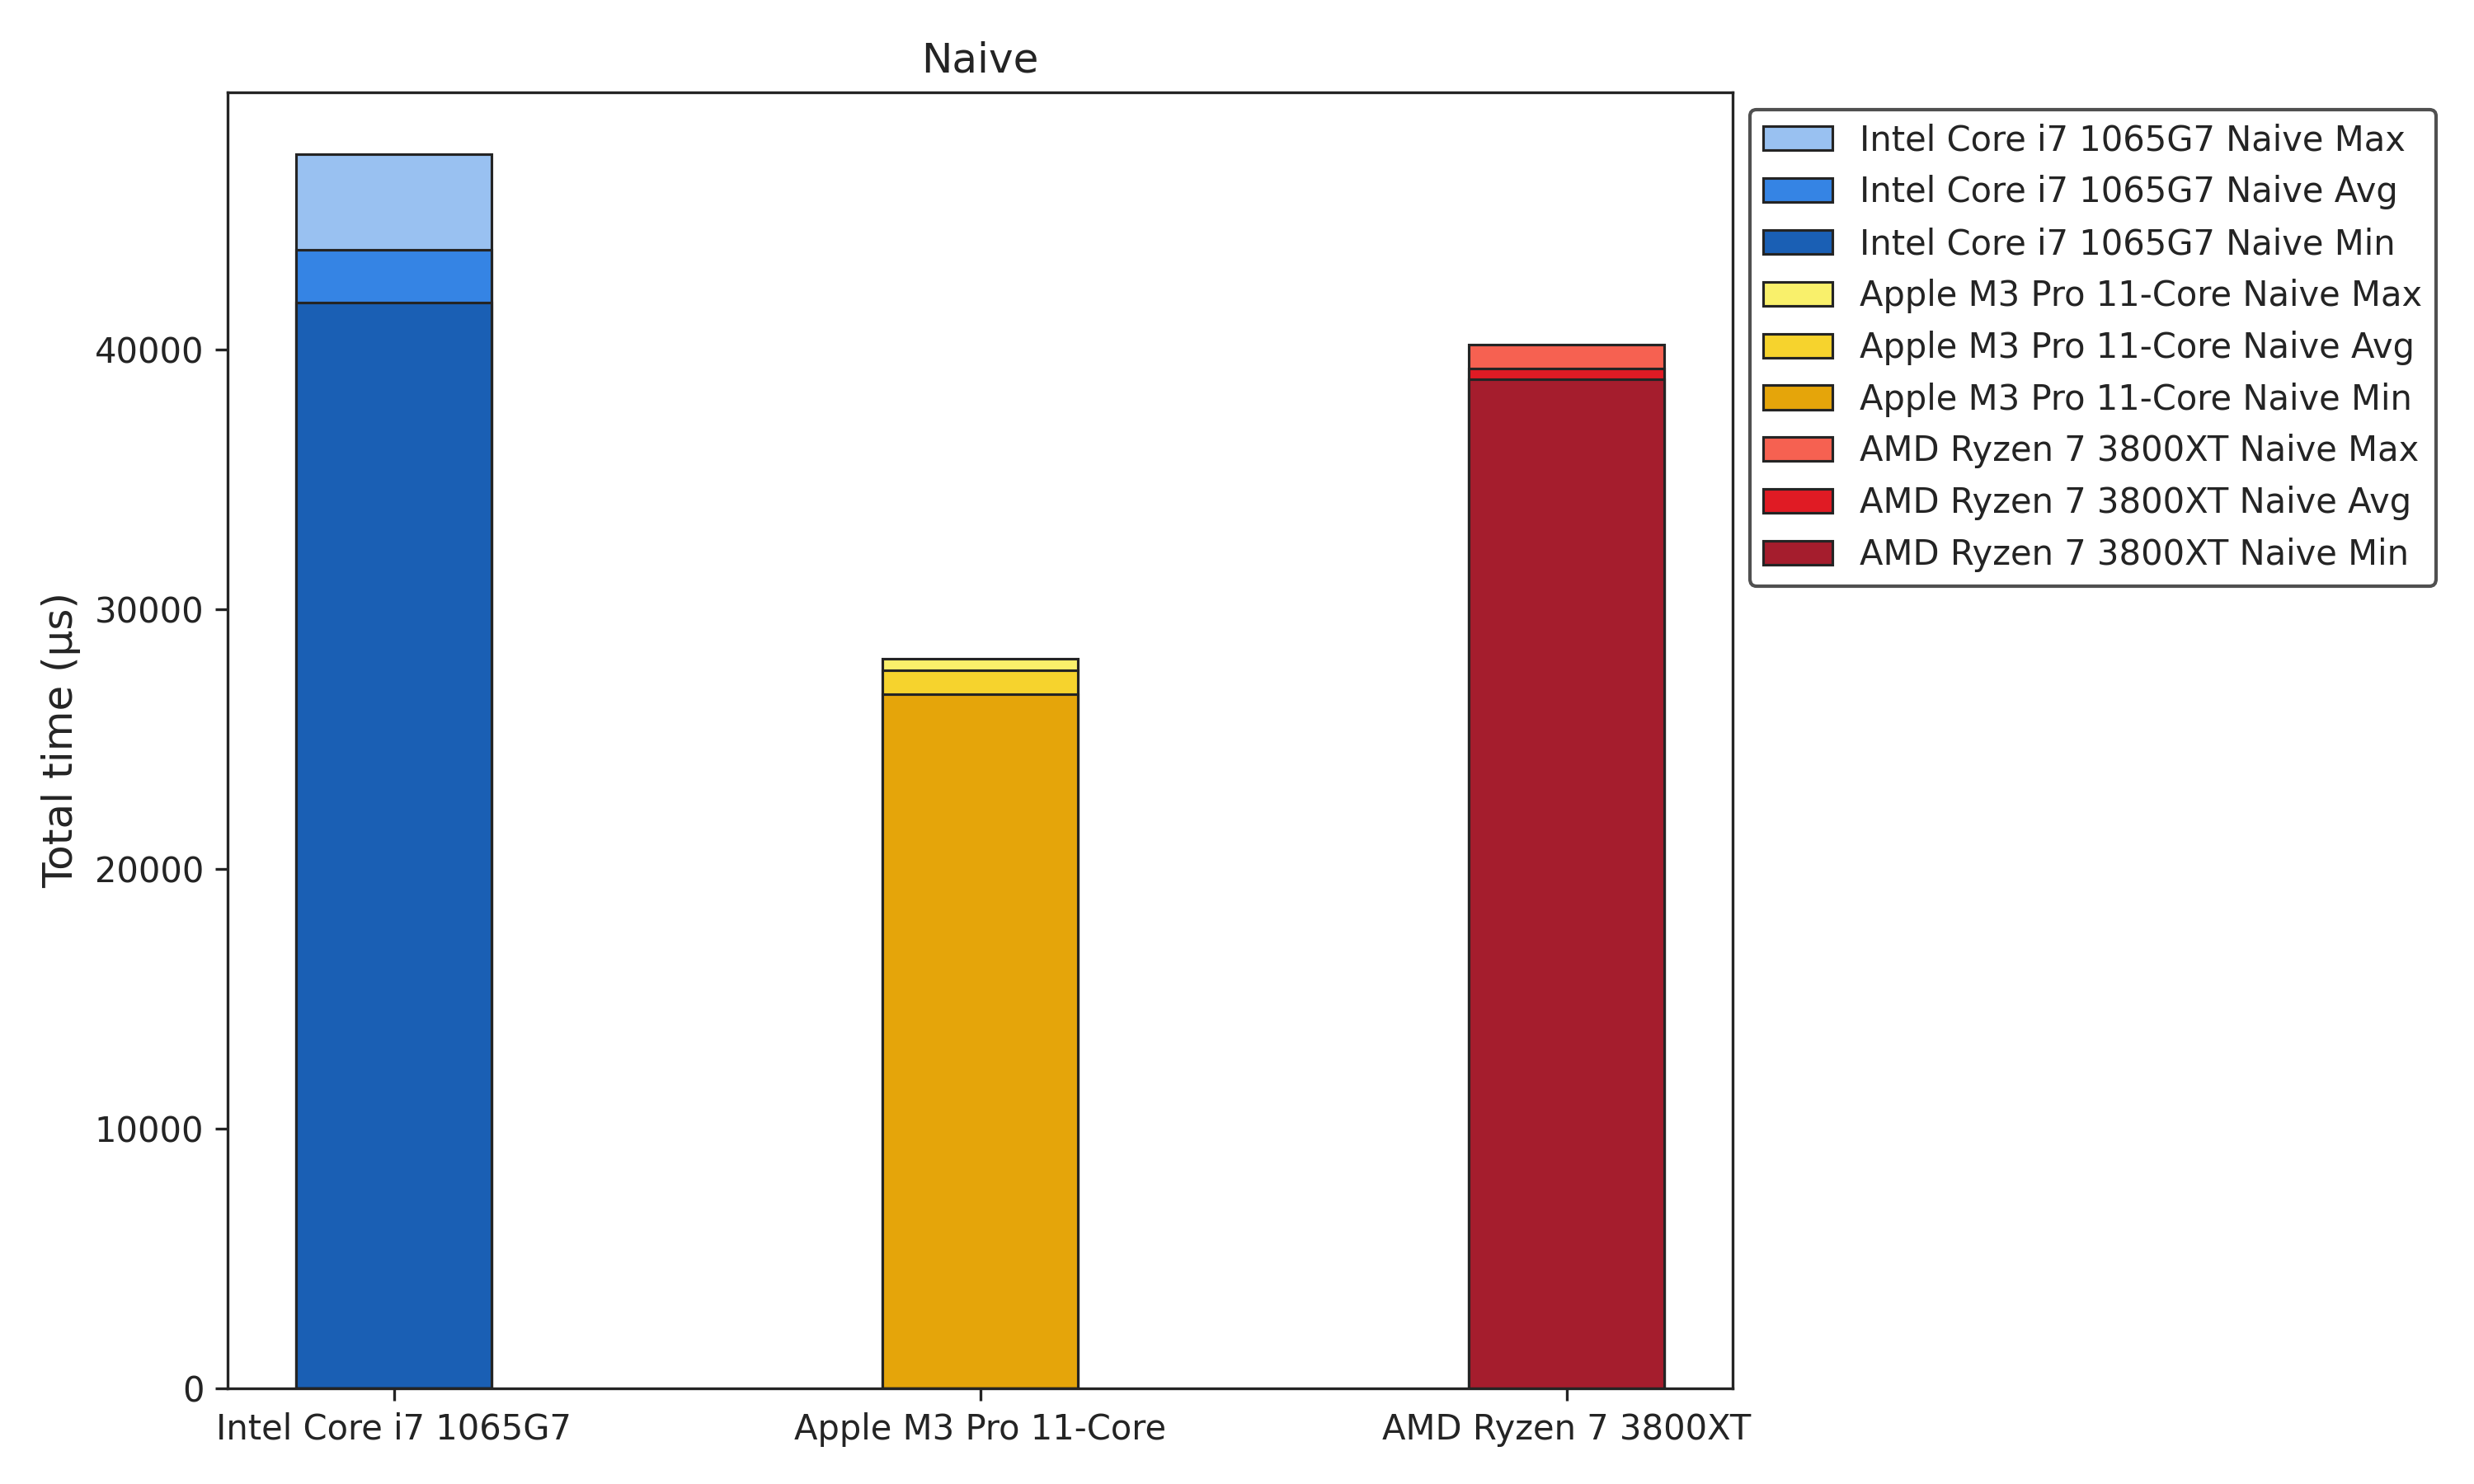
\includegraphics[width=\linewidth]{Graphs/Naive.png}
  \caption{On the MNIST dataset}
 \label{fig:naive_mnist}
\end{subfigure}%
\begin{subfigure}{.5\textwidth}
  \centering
  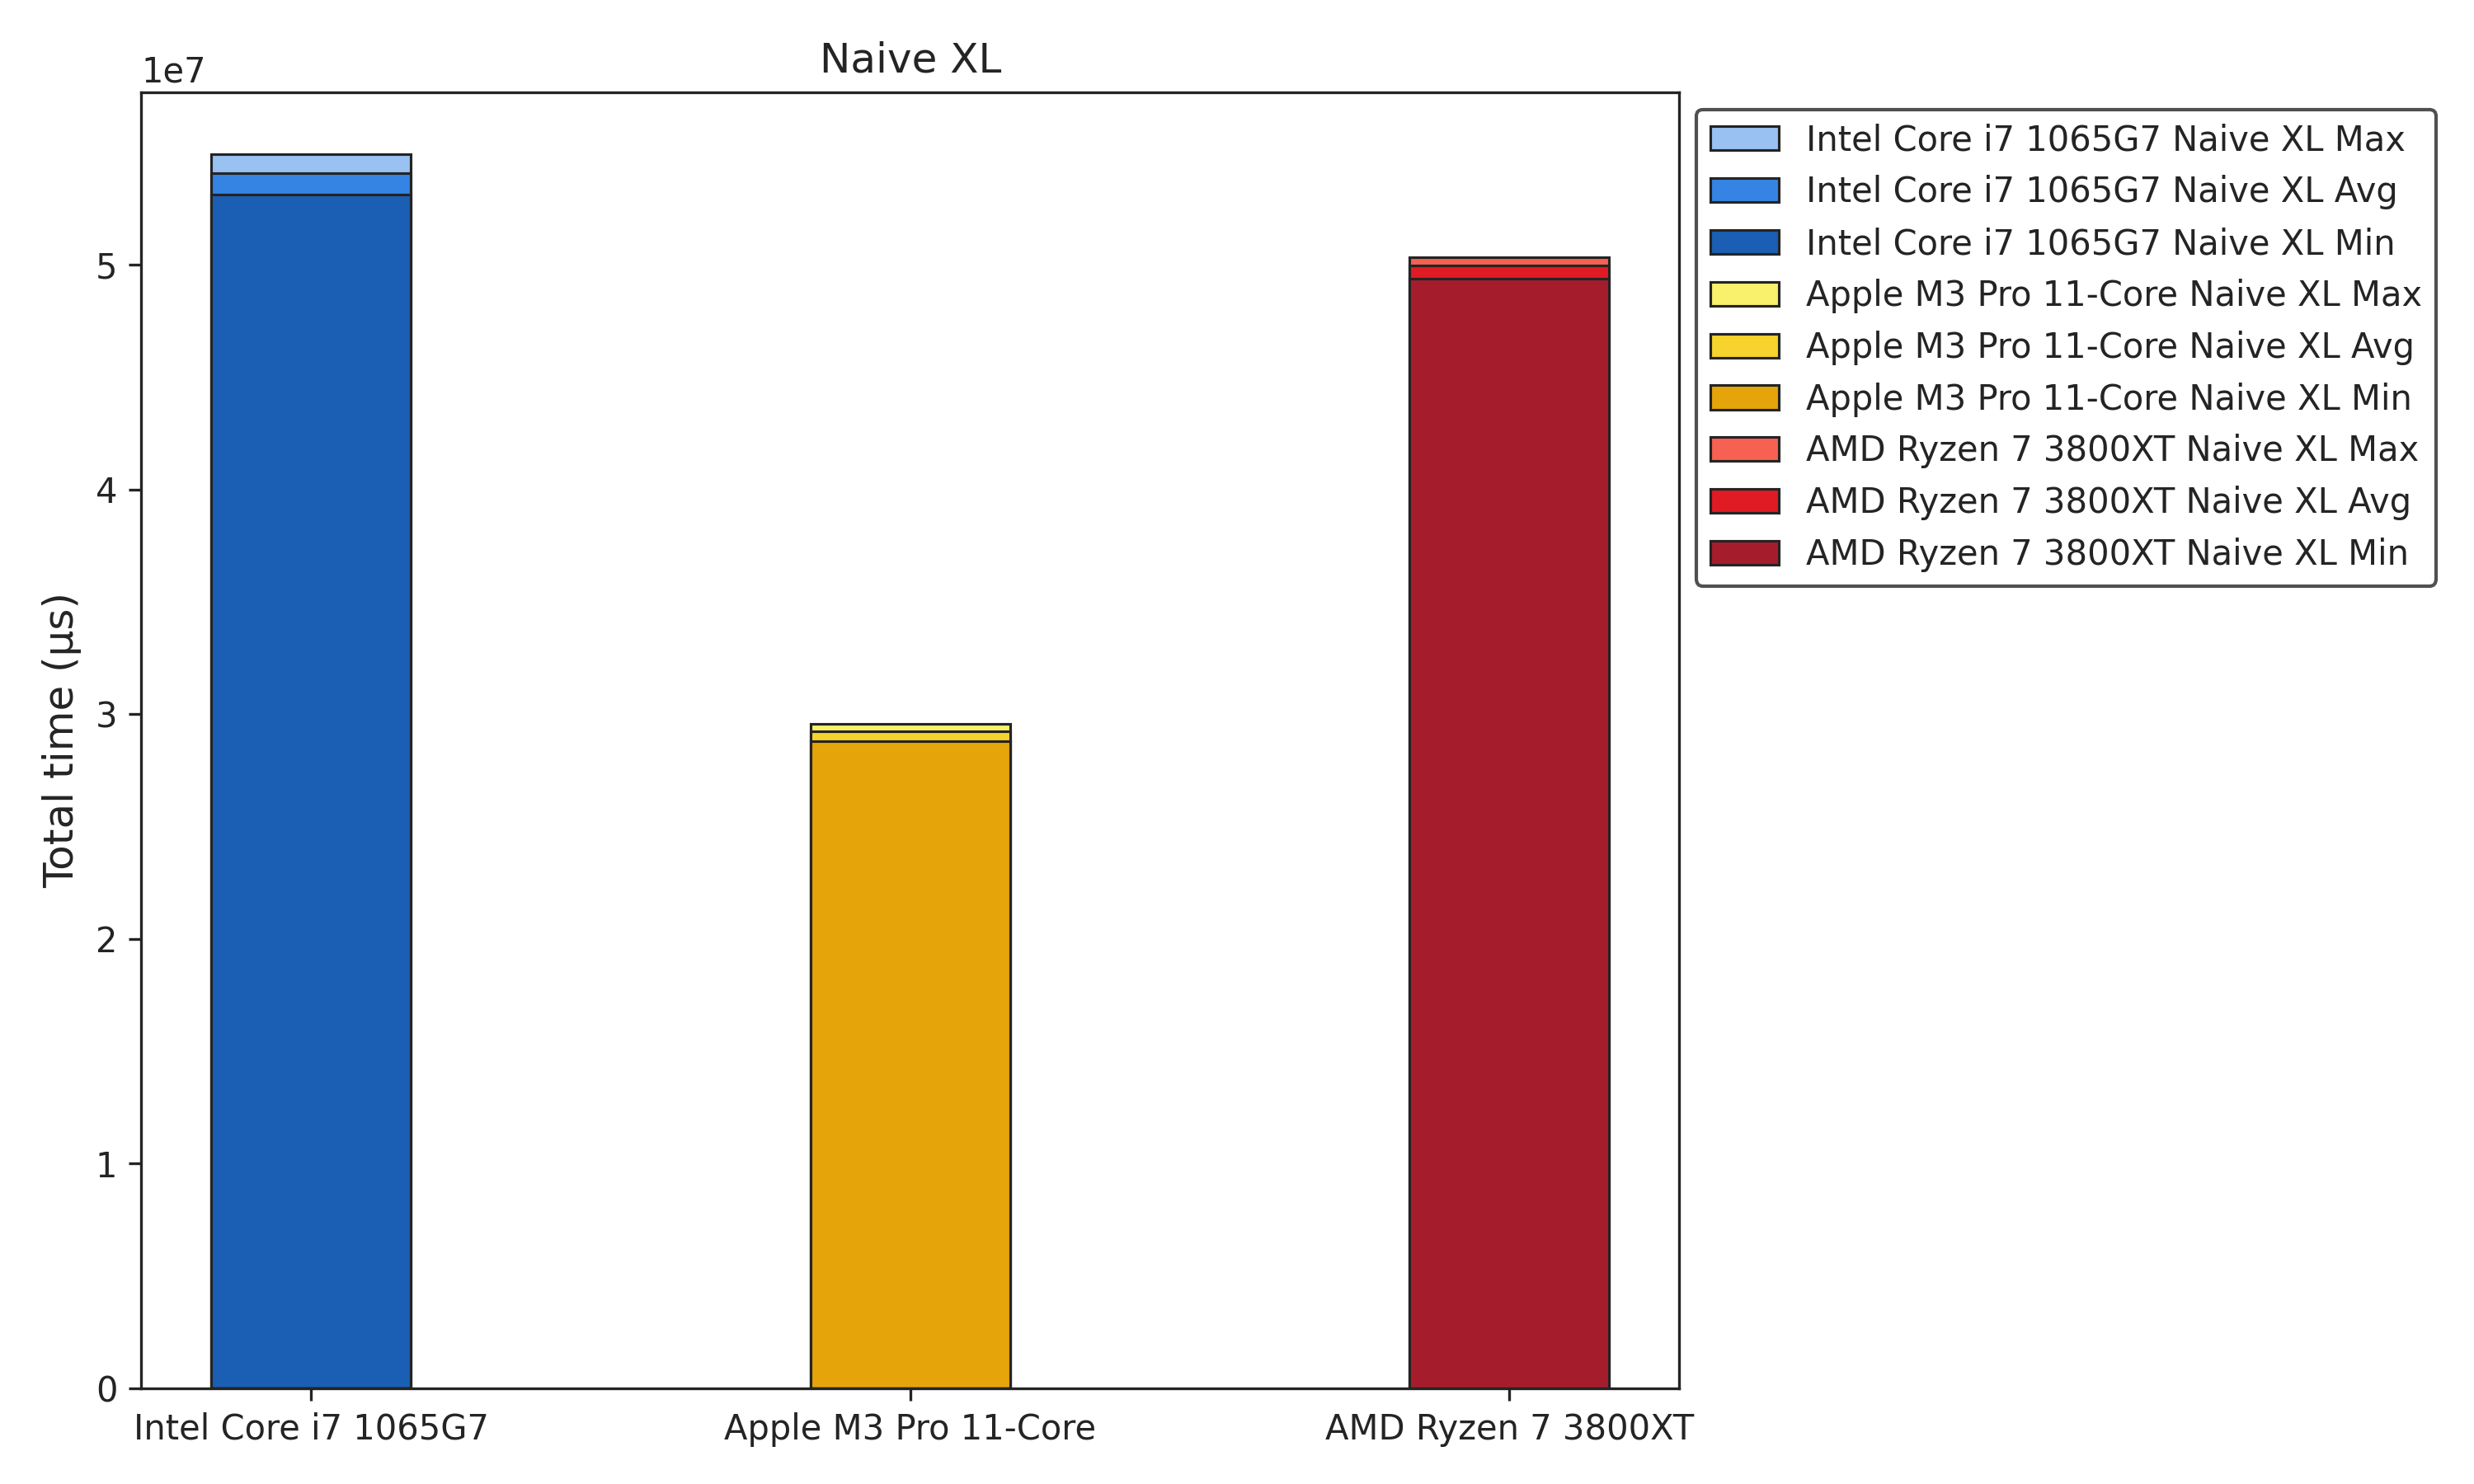
\includegraphics[width=\linewidth]{Graphs/Naive XL.png}
  \caption{On the synthetic XL dataset}
 \label{fig:naive_xl}
\end{subfigure}
\caption{Performance benchmarks of the naive implementation}
\label{fig:naive}
\end{figure}
\begin{table}[htb!]
\centering
\caption{Naive Implementation\label{tab:naive}}
\begin{tabular}{p{5cm} p{2cm} p{2cm} p{2cm} p{2cm}}
\hline
Benchmark Name & Minimum Value ($\mu$s) & Average Value ($\mu$s) & Maximum Value ($\mu$s) & Standard Deviation \\
\hline
Intel Core i7-1065G7 \\
\hspace{0.5cm}Naive & 41783.0 & 43833.5 & 47517.0 & 1788.0 \\
Apple M3 Pro 11-Core \\
\hspace{0.5cm}Naive & 26718.0 & 27648.4 & 28075.0 & 468.9 \\
AMD Ryzen 7 3800XT \\
\hspace{0.5cm}Naive & 38841.0 & 39271.6 & 40180.0 & 379.2 \\
\hline
Intel Core i7-1065G7 \\
\hspace{0.5cm}Naive XL & 53137471.0 & 54097305.1 & 54939589.0 & 549782.2 \\
Apple M3 Pro 11-Core \\
\hspace{0.5cm}Naive XL & 28821610.0 & 29244264.5 & 29572155.0 & 226548.1 \\
AMD Ryzen 7 3800XT \\
\hspace{0.5cm}Naive XL & 49407386.0 & 49970509.5 & 50337761.0 & 318289.1 \\
\hline
\end{tabular}
\end{table}
\FloatBarrier

Apple Silicon represents by far the most recent processor in this comparison and clearly delivers the best performance—nearly twice as high as that of the other two CPUs. The performance gap between the remaining processors is significantly smaller, which can be reasonably explained by their release dates and power consumption. With its newly developed architecture, Apple effectively revolutionizes the market and demonstrates an unprecedented performance-per-watt ratio. We do not expect our optimizations to alter the ranking of the processors and will therefore focus primarily on the relative changes within the context of each individual CPU.
\section{CPU-Based Optimizations}\label{sec:cpu-based-optimizations}
\subsection{Multithreading}\label{sec:multithreading}
Figure~\ref{fig:multithreading_concepts} offers a helpful diagram that illustrates the concepts covered in this chapter.
\begin{figure}[htb!]
    \centering
    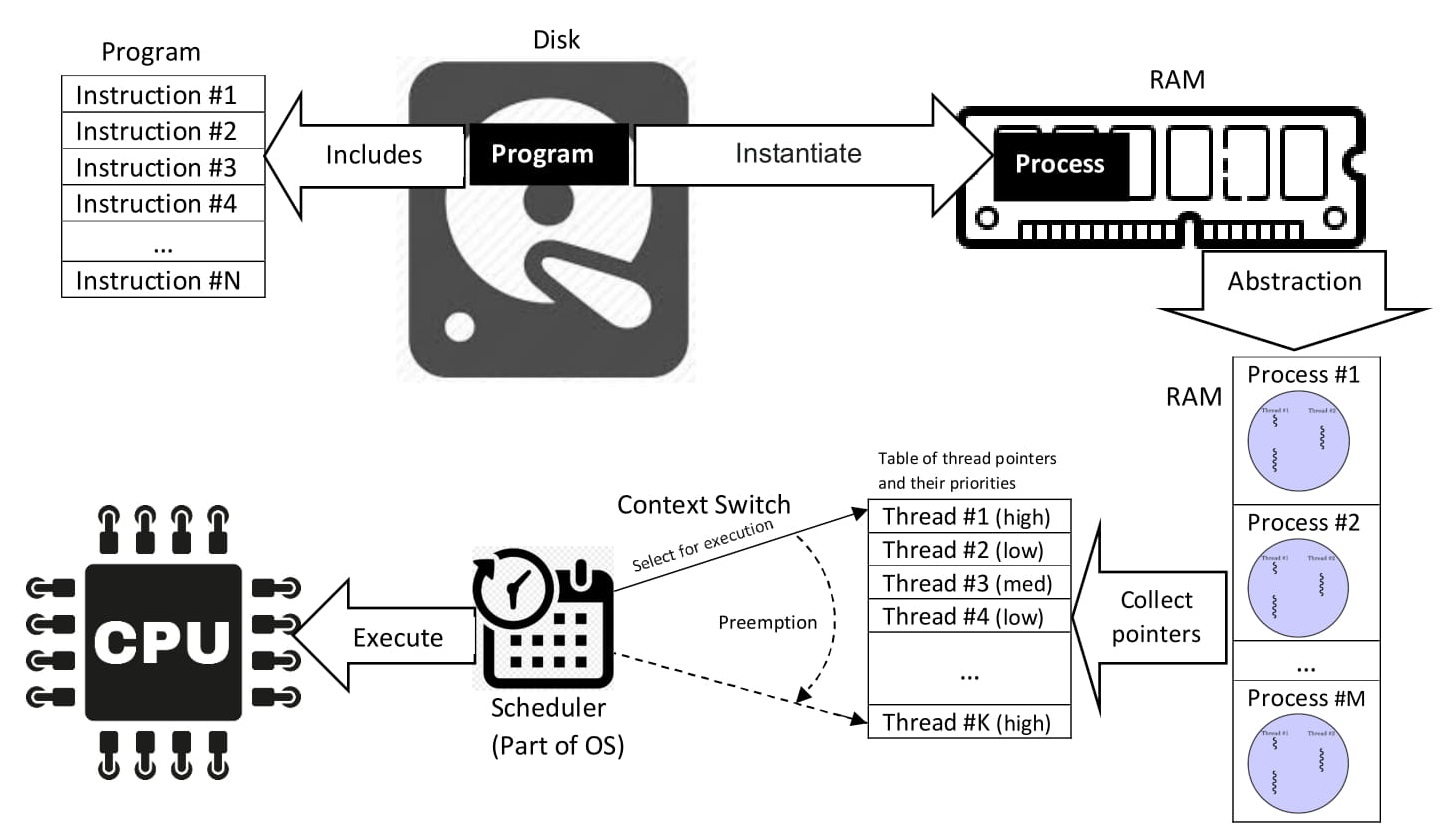
\includegraphics[width=\linewidth]{Multithreading/Concepts-_Program_vs._Process_vs._Thread.jpg}
    \caption{Program vs. Process vs. Thread Scheduling, Preemption, Context Switching\footnote{Thread (computing): \url{https://en.wikipedia.org/wiki/Thread_(computing)} (accessed April 14, 2025).}}
   \label{fig:multithreading_concepts}
\end{figure}
\subsubsection{Overview}
As the first optimization, we focus on multithreading. However, we are not referring to the type of multithreading used by the operating system's scheduler, which switches to another task when the current process is wasting valuable computation time while waiting for input/output. Instead, we refer to the multithreading enabled by the computer architecture itself, as all CPUs used in this paper are designed with multiple physical cores that can operate independently and in parallel. Intel and AMD CPUs also offer Simultaneous Multithreading (SMT), called Hyper-Threading (HT) on Intel processors\footnote{Characterization of multithreaded scientific workloads on simultaneous multithreading intel processors: \url{https://citeseerx.ist.psu.edu/document?repid=rep1&type=pdf&doi=34cc0f6b6cdb71f95b742fd409861061542112c7} (Grant, Ryan E., and Ahmad Afsahi, 2005)}, which provides twice as many threads as there are physical cores. The Intel Core i7-1065G7 has 4 physical cores but 8 threads, and the AMD Ryzen 7 3800XT has 8 physical cores but 16 threads. We refer to these additional cores as threads because they are not truly independent; they share execution units (e.g., ALUs, FPUs) and the L1 cache, although the logical registers remain separate. This allows one thread to perform addition while another performs multiplication.

Apple Silicon does not support SMT; instead, it divides the cores into performance and efficiency cores. The performance cores are based on the latest architecture, are manufactured with the most advanced process, and offer the highest frequencies. In contrast, efficiency cores are typically based on older architecture and manufacturing processes, and they are often downclocked. The design of efficiency cores reduces heat and power consumption, minimizing the need for cooling and extending battery life, while allowing the performance cores to focus on more demanding tasks without handling smaller ones. The Apple M3 Pro 11-core chip consists of 5 performance cores and 6 efficiency cores, with one performance core disabled due to a manufacturing defect, making it a binned version, in comparison to the full 12-core version that has 6 performance cores.

With multithreading, a speedup of up to the number of cores is theoretically achievable. However, real-world programs always have a sequential portion that cannot be parallelized, for instance, due to data dependencies within a loop, meaning that we do not expect to achieve the full theoretical speedup. Nevertheless, we aim to get as close to this limit as possible. With this optimization, we expect that as many functions as possible will execute a large portion of their tasks in parallel rather than sequentially. As a result, we anticipate that the current CPU load, which is 20\% on a single core, will increase to 100\% across all cores, fully utilizing the CPU's potential and thus improving performance by reducing total execution time. We also expect better scalability of our framework for larger problem sizes, avoiding the exponential increase in execution time that we currently experience.

For the implementation, we choose POSIX Threads (Pthreads), a standardized API for managing threads, which works cross-platform on most Unix-like systems, including Linux and macOS. This is particularly important because, at the time of creating the framework, no Asahi Linux version was available for the MacBook being used. The API provides tools for creating, managing, and synchronizing threads. Additionally, we are already familiar with Pthreads, and its extensive documentation will speed up the development process.\footnote{Programming with POSIX Threads: \url{https://books.google.de/books?id=TXiJDj9kbiAC&lpg=PR7} (David R. Butenhof, 1993)}
\subsubsection{Initial Implementation}
After providing an overview of multithreading and selecting an appropriate API, we proceed to the proof of concept. This step involves verifying that the code sections identified as suitable for multithreading can indeed be parallelized without compromising accuracy, ensuring that the calculations remain correct. We implement multithreading across all ten functions of our custom TensorFlow module. Helper functions, which are typically single-line and inherently sequential, as well as the loading of weights and images, are not parallelized. 

In the initial implementation, each function manages its own threads, starting them after each function call and joining them again before returning. While this approach allows us to verify functionality, the overhead is disproportionate to the potential speedup. As a result, the performance becomes significantly worse than expected, with benchmarks showing a severe decline. 

Thanks to a suggestion from Philipp Holzinger, we quickly switch to using a thread pool. In a thread pool, threads are managed globally. They are created once at the beginning and joined only once at the end, greatly reducing the overhead previously encountered. This behavior represents the industry standard for multithreading. Unlike the initial implementation, threads are no longer directly assigned to specific tasks; instead, they enter an ongoing loop. Tasks are now managed through a GLib thread-safe queue.

GLib 2.85 is a general-purpose, portable utility library that offers a variety of useful features, such as data types, macros, type conversions, string utilities, file utilities, and a main loop abstraction, among others.\footnote{GLib – 2.0: \url{https://docs.gtk.org/glib/} (accessed April 14, 2025).} In this new setup, the previously used functions now act as managers. They place one of the new helper functions into the queue with their parameters and wait for the thread pool to successfully execute the task before returning the result. The queue holds a specially defined struct, named mt\_arg, which contains various data, including the thread index in the pool, pointers to input and output matrices, and a pointer to a helper function. This function performs the algorithm required by the respective function, using the passed parameters. 

The matrices are stored in memory and shared among all threads, eliminating any additional copy overhead. We ensure that each thread only accesses its disjoint portion of the memory, preventing race conditions. To return the correct result, synchronization and writing back occur only once. When a task is added to the queue, the threads in the pool wake up, execute the task, and then return to a sleeping state until a new task arrives. This approach improves the performance of sequential parts, as the operating system scheduler no longer wastes time slots on a process waiting in an infinite loop.

To enable the threads to be joined, we develop a poison pill mechanism. This mechanism behaves like any other task and is placed in the queue. When executed by the thread pool, it allows a thread to terminate and be joined. By doing so, we avoid unnecessary conditional checks and potential branch mispredictions while still providing a way to cleanly terminate threads.
\subsubsection{Performance Benchmarks}
The benchmark results are shown in Figure~\ref{fig:initial_multithreading}, with the corresponding values listed in Table~\ref{tab:initial_multithreading}. The average performance of all CPUs on the MNIST dataset decreases by 457.7\%. The average performance of the Intel Core i7-1065G7 decreases by 202.9\%, the Apple M3 Pro 11-Core decreases by 631.9\%, and the AMD Ryzen 7 3800XT decreases by 619.6\%. The average performance of all CPUs on the synthetic XL dataset improves by 22.4\%. The Intel Core i7-1065G7 improves by 16.8\%, the Apple M3 Pro 11-Core improves by 39.9\%, and the AMD Ryzen 7 3800XT improves by 18.2\%.
\begin{figure}[htb!]
\centering
\begin{subfigure}{.5\textwidth}
  \centering
  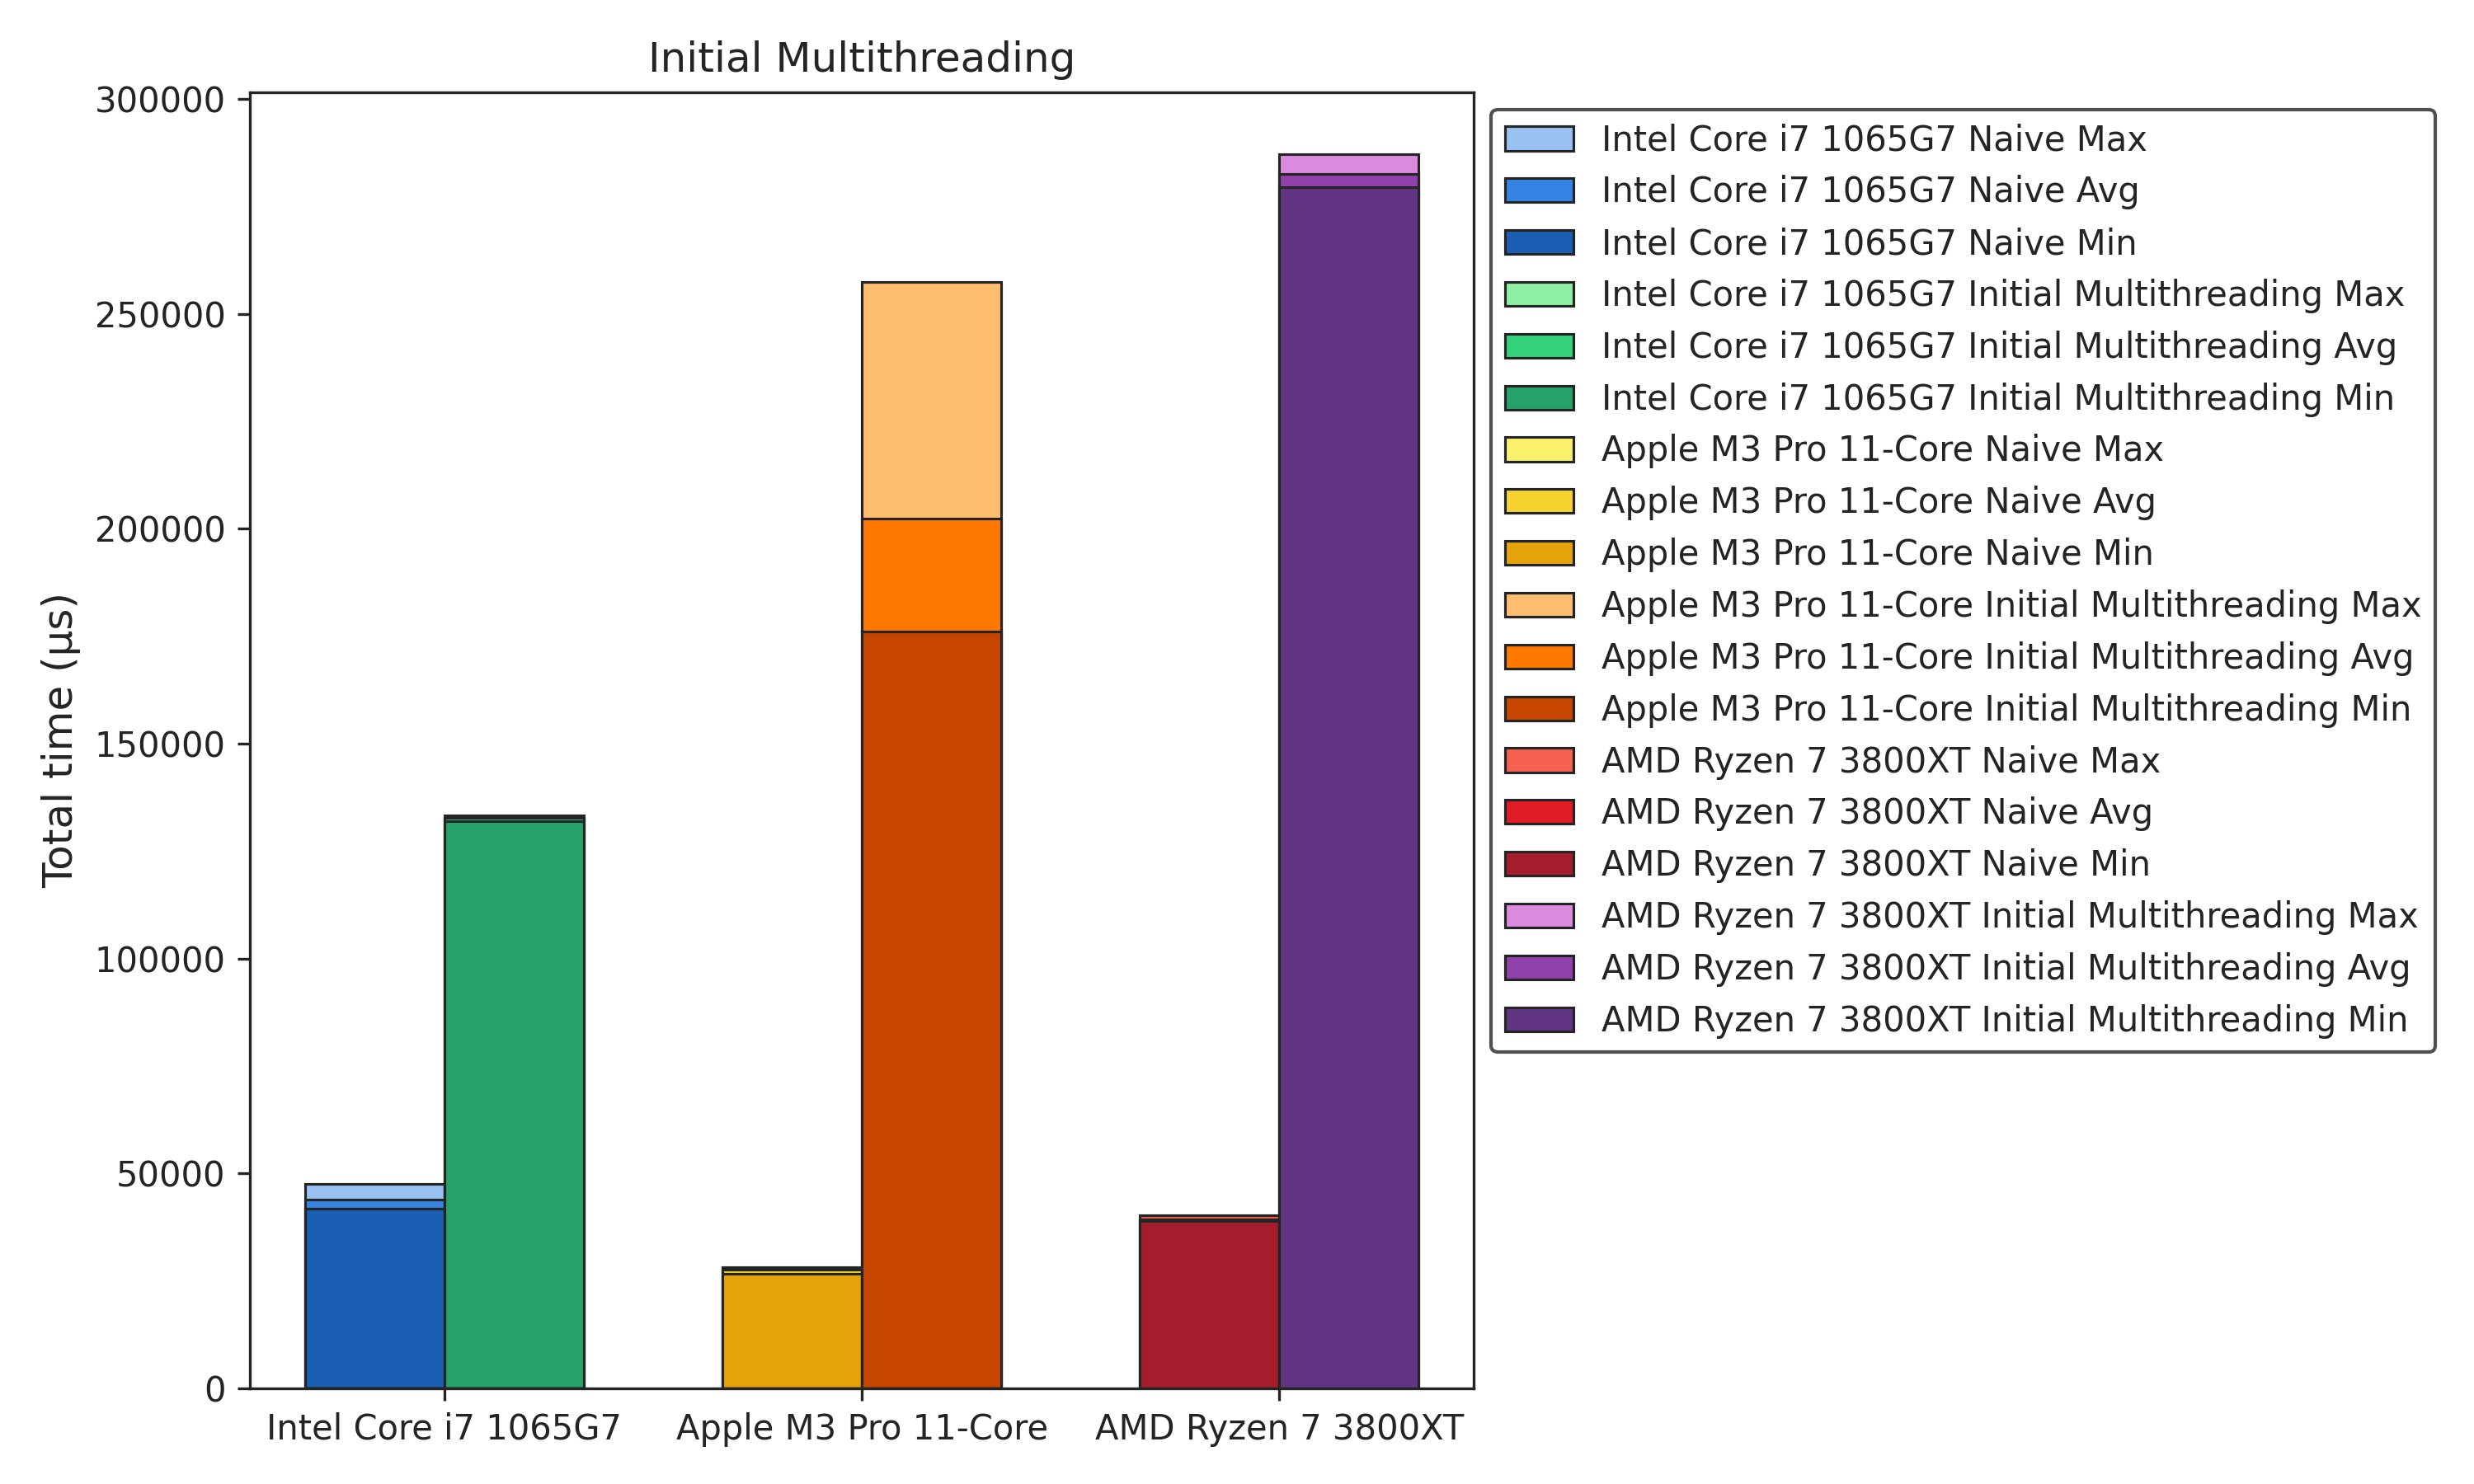
\includegraphics[width=\linewidth]{Graphs/Initial Multithreading.png}
  \caption{On the MNIST dataset}
 \label{fig:initial_multithreading_mnist}
\end{subfigure}%
\begin{subfigure}{.5\textwidth}
  \centering
  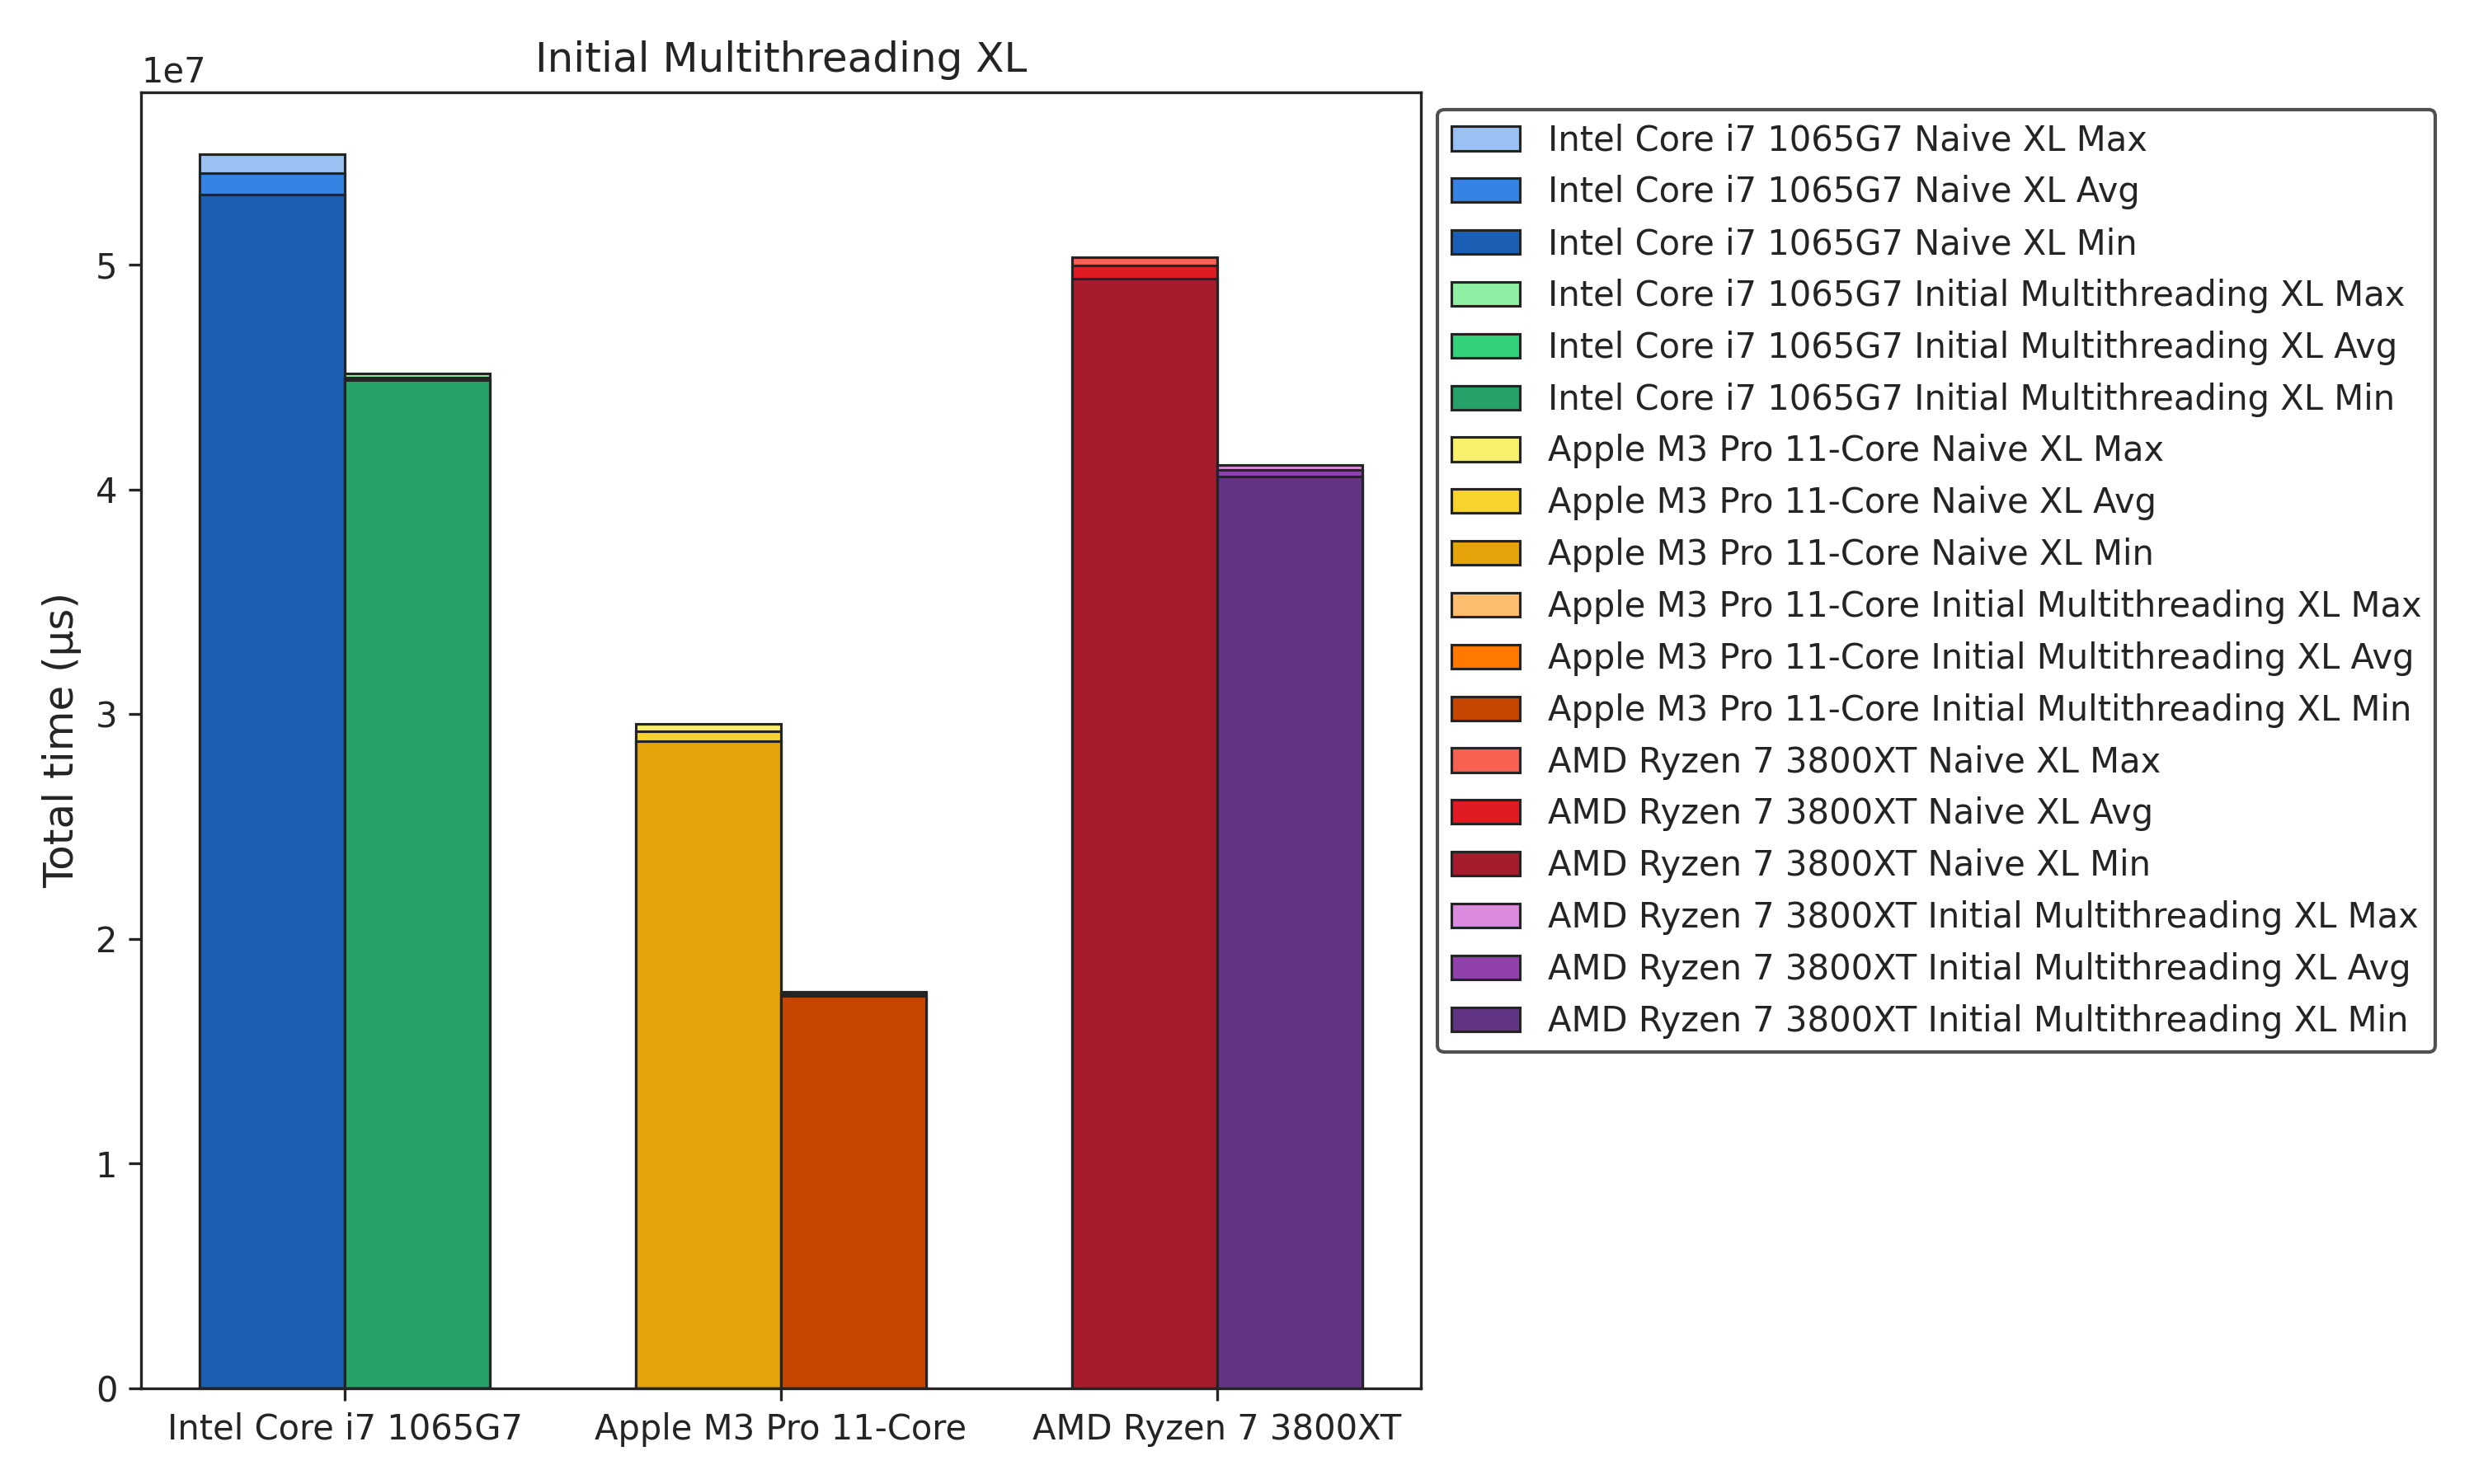
\includegraphics[width=\linewidth]{Graphs/Initial Multithreading XL.png}
  \caption{On the synthetic XL dataset}
 \label{fig:initial_multithreading_xl}
\end{subfigure}
\caption{Performance benchmarks of the initial multithreading implementation}
\label{fig:initial_multithreading}
\end{figure}
\begin{table}[htb!]
\centering
\caption{Initial Multithreading Implementation\label{tab:initial_multithreading}}
\begin{tabular}{p{5cm} p{2cm} p{2cm} p{2cm} p{2cm}}
\hline
Benchmark Name & Minimum Value ($\mu$s) & Average Value ($\mu$s) & Maximum Value ($\mu$s) & Standard Deviation \\
\hline
Intel Core i7-1065G7 \\
\hspace{0.5cm}Naive & 41783.0 & 43833.5 & 47517.0 & 1788.0 \\
\hspace{0.5cm}Initial Multithreading & 131866.0 & 132756.0 & 133229.0 & 366.1 \\
Apple M3 Pro 11-Core \\
\hspace{0.5cm}Naive & 26718.0 & 27648.4 & 28075.0 & 468.9 \\
\hspace{0.5cm}Initial Multithreading & 176040.0 & 202359.7 & 257459.0 & 21555.6 \\
AMD Ryzen 7 3800XT \\
\hspace{0.5cm}Naive & 38841.0 & 39271.6 & 40180.0 & 379.2 \\
\hspace{0.5cm}Initial Multithreading & 279513.0 & 282589.0 & 287196.0 & 2643.1 \\
\hline
Intel Core i7-1065G7 \\
\hspace{0.5cm}Naive XL & 53137471.0 & 54097305.1 & 54939589.0 & 549782.2 \\
\hspace{0.5cm}Initial Multithreading XL & 44870433.0 & 45002714.3 & 45163577.0 & 102509.7 \\
Apple M3 Pro 11-Core \\
\hspace{0.5cm}Naive XL & 28821610.0 & 29244264.5 & 29572155.0 & 226548.1 \\
\hspace{0.5cm}Initial Multithreading XL & 17466123.0 & 17567938.9 & 17641156.0 & 61687.5 \\
AMD Ryzen 7 3800XT \\
\hspace{0.5cm}Naive XL & 49407386.0 & 49970509.5 & 50337761.0 & 318289.1 \\
\hspace{0.5cm}Initial Multithreading XL & 40573406.0 & 40867988.9 & 41106348.0 & 185968.0 \\
\hline
\end{tabular}
\end{table}
\FloatBarrier

As evident, the results are truly dreadful—far from what is expected or desired. The initial multithreading implementation clearly illustrates that well-intentioned but poorly executed optimizations can actually degrade performance rather than improve it.

In investigating the causes behind this disappointing outcome, several key issues have been identified:

First, we parallelize all ten functions of our custom TensorFlow module. While this sounds promising in theory, on the MNIST dataset it proves highly inefficient. Many of these functions, such as flipping kernels, operate on small 3x3 matrices. Naturally, the computational workload here is far too low to justify the overhead introduced by multithreading.

Second, the custom struct we enqueue contains many avoidable elements, making it unnecessarily large. This significantly increases both memory usage and the associated copy overhead.

Third, our current method of distributing work across threads alternates task assignments in a way that negates all potential cache benefits, leading to further inefficiencies.

Fourth, our current codebase does not support multithreading at the image level and remains quite rudimentary overall.

These issues collectively explain the poor performance. However, identifying these problems allows us to now focus on developing and implementing targeted solutions.

Interestingly, despite the aforementioned limitations observed with the MNIST dataset, we already observe performance improvements on the synthetic XL dataset. This indicates that our implementation benefits from scale, at least in this context. With further optimization of the MNIST processing, we expect a substantial performance gain on the synthetic dataset as well.
\subsubsection{Optimized Implementation}\label{subsec:optimized-implementation}
After executing the benchmarks, analyzing the results, and identifying possible reasons for failure, we now proceed to the design and resolution phase. We approach this step by step.

We begin with the issue that many functions are called with matrices that are too small, resulting in insufficient workload to justify the overhead of multithreading. Since our goal is to develop a general-purpose framework, enforcing single-threading for such functions is not a viable solution. For instance, a larger artificial intelligence model might use 100x100 masks, in which case multithreading flip kernels is indeed beneficial.

We therefore implement a smart multithreading strategy. This approach dynamically checks whether the axis being split during multithreading is sufficiently large relative to the selected number of threads. Although this introduces an additional condition that could potentially cause branch mispredictions, our tests show that this trade-off is reasonable. While more sophisticated implementations of smart multithreading likely exist, our primitive version already achieves the desired effect.

Next, we reduce the size of the mt\_arg struct, which is used for the queue. This struct previously contained many redundant elements, making it unnecessarily large. Since each function call results in the creation, population, and copying of multiple such structs—one for each thread—the overhead from copying accumulates quickly. Our solution involves removing unused variables, converting long values to int, avoiding padding, and replacing all potential input and output parameter configurations with three generic void pointers. Although this requires careful handling and explicit casting, the compromise proves acceptable in testing. While the struct remains relatively large and still represents the largest portion of the framework’s memory footprint, these optimizations reduce its size by more than half. Moreover, the number of structs created is further reduced thanks to the aforementioned smart multithreading.

We then address an unintended issue: the complete loss of cache efficiency. All modern CPUs—including those used in our benchmarks—support prefetching. Rather than loading a single value, entire cache lines are fetched under the assumption that adjacent values will soon be needed. This improves performance by making data available before it is explicitly requested by the program. However, our current alternating thread distribution disrupts this mechanism: the next value that is prefetched is never used, and each thread ends up fetching a completely new cache line repeatedly, wasting memory bandwidth and reducing performance.

To resolve this, we implement cache blocking. Elements are now distributed to threads in contiguous blocks, maximizing cache reuse and significantly improving performance through effective use of prefetching.\footnote{When prefetching works, when it doesn’t, and why: \url{https://dl.acm.org/doi/pdf/10.1145/2133382.2133384} (Lee, Jaekyu, Hyesoon Kim, and Richard Vuduc, 2012)}

Finally, we migrate our current primitive and fragmented multithreading implementation, which is spread across multiple files, into a unified C++ class. This enables the flexible creation of objects and allows us to implement multithreading on top of already multithreaded functions—a level of parallelism that was previously impossible. To retain the ability to queue function pointers, we create wrapper functions for each target function that accept an object instance as a parameter.

With these improvements, we address all issues previously identified and now expect to achieve the excellent performance we originally anticipated during the initial implementation.
\subsubsection{Performance Benchmarks}
The benchmark results are shown in Figure~\ref{fig:multithreading}, with the corresponding values listed in Table~\ref{tab:multithreading}. The average performance of all CPUs on the MNIST dataset improves by 92.8\%. The average performance of the Intel Core i7-1065G7 improves by 91.6\%, the Apple M3 Pro 11-Core improves by 94.2\%, and the AMD Ryzen 7 3800XT improves by 92.4\%. The average performance of all CPUs on the synthetic XL dataset improves by 81.7\%. The Intel Core i7-1065G7 improves by 80.8\%, the Apple M3 Pro 11-Core improves by 83.7\%, and the AMD Ryzen 7 3800XT improves by 81.8\%.
\begin{figure}[htb!]
\centering
\begin{subfigure}{.5\textwidth}
  \centering
  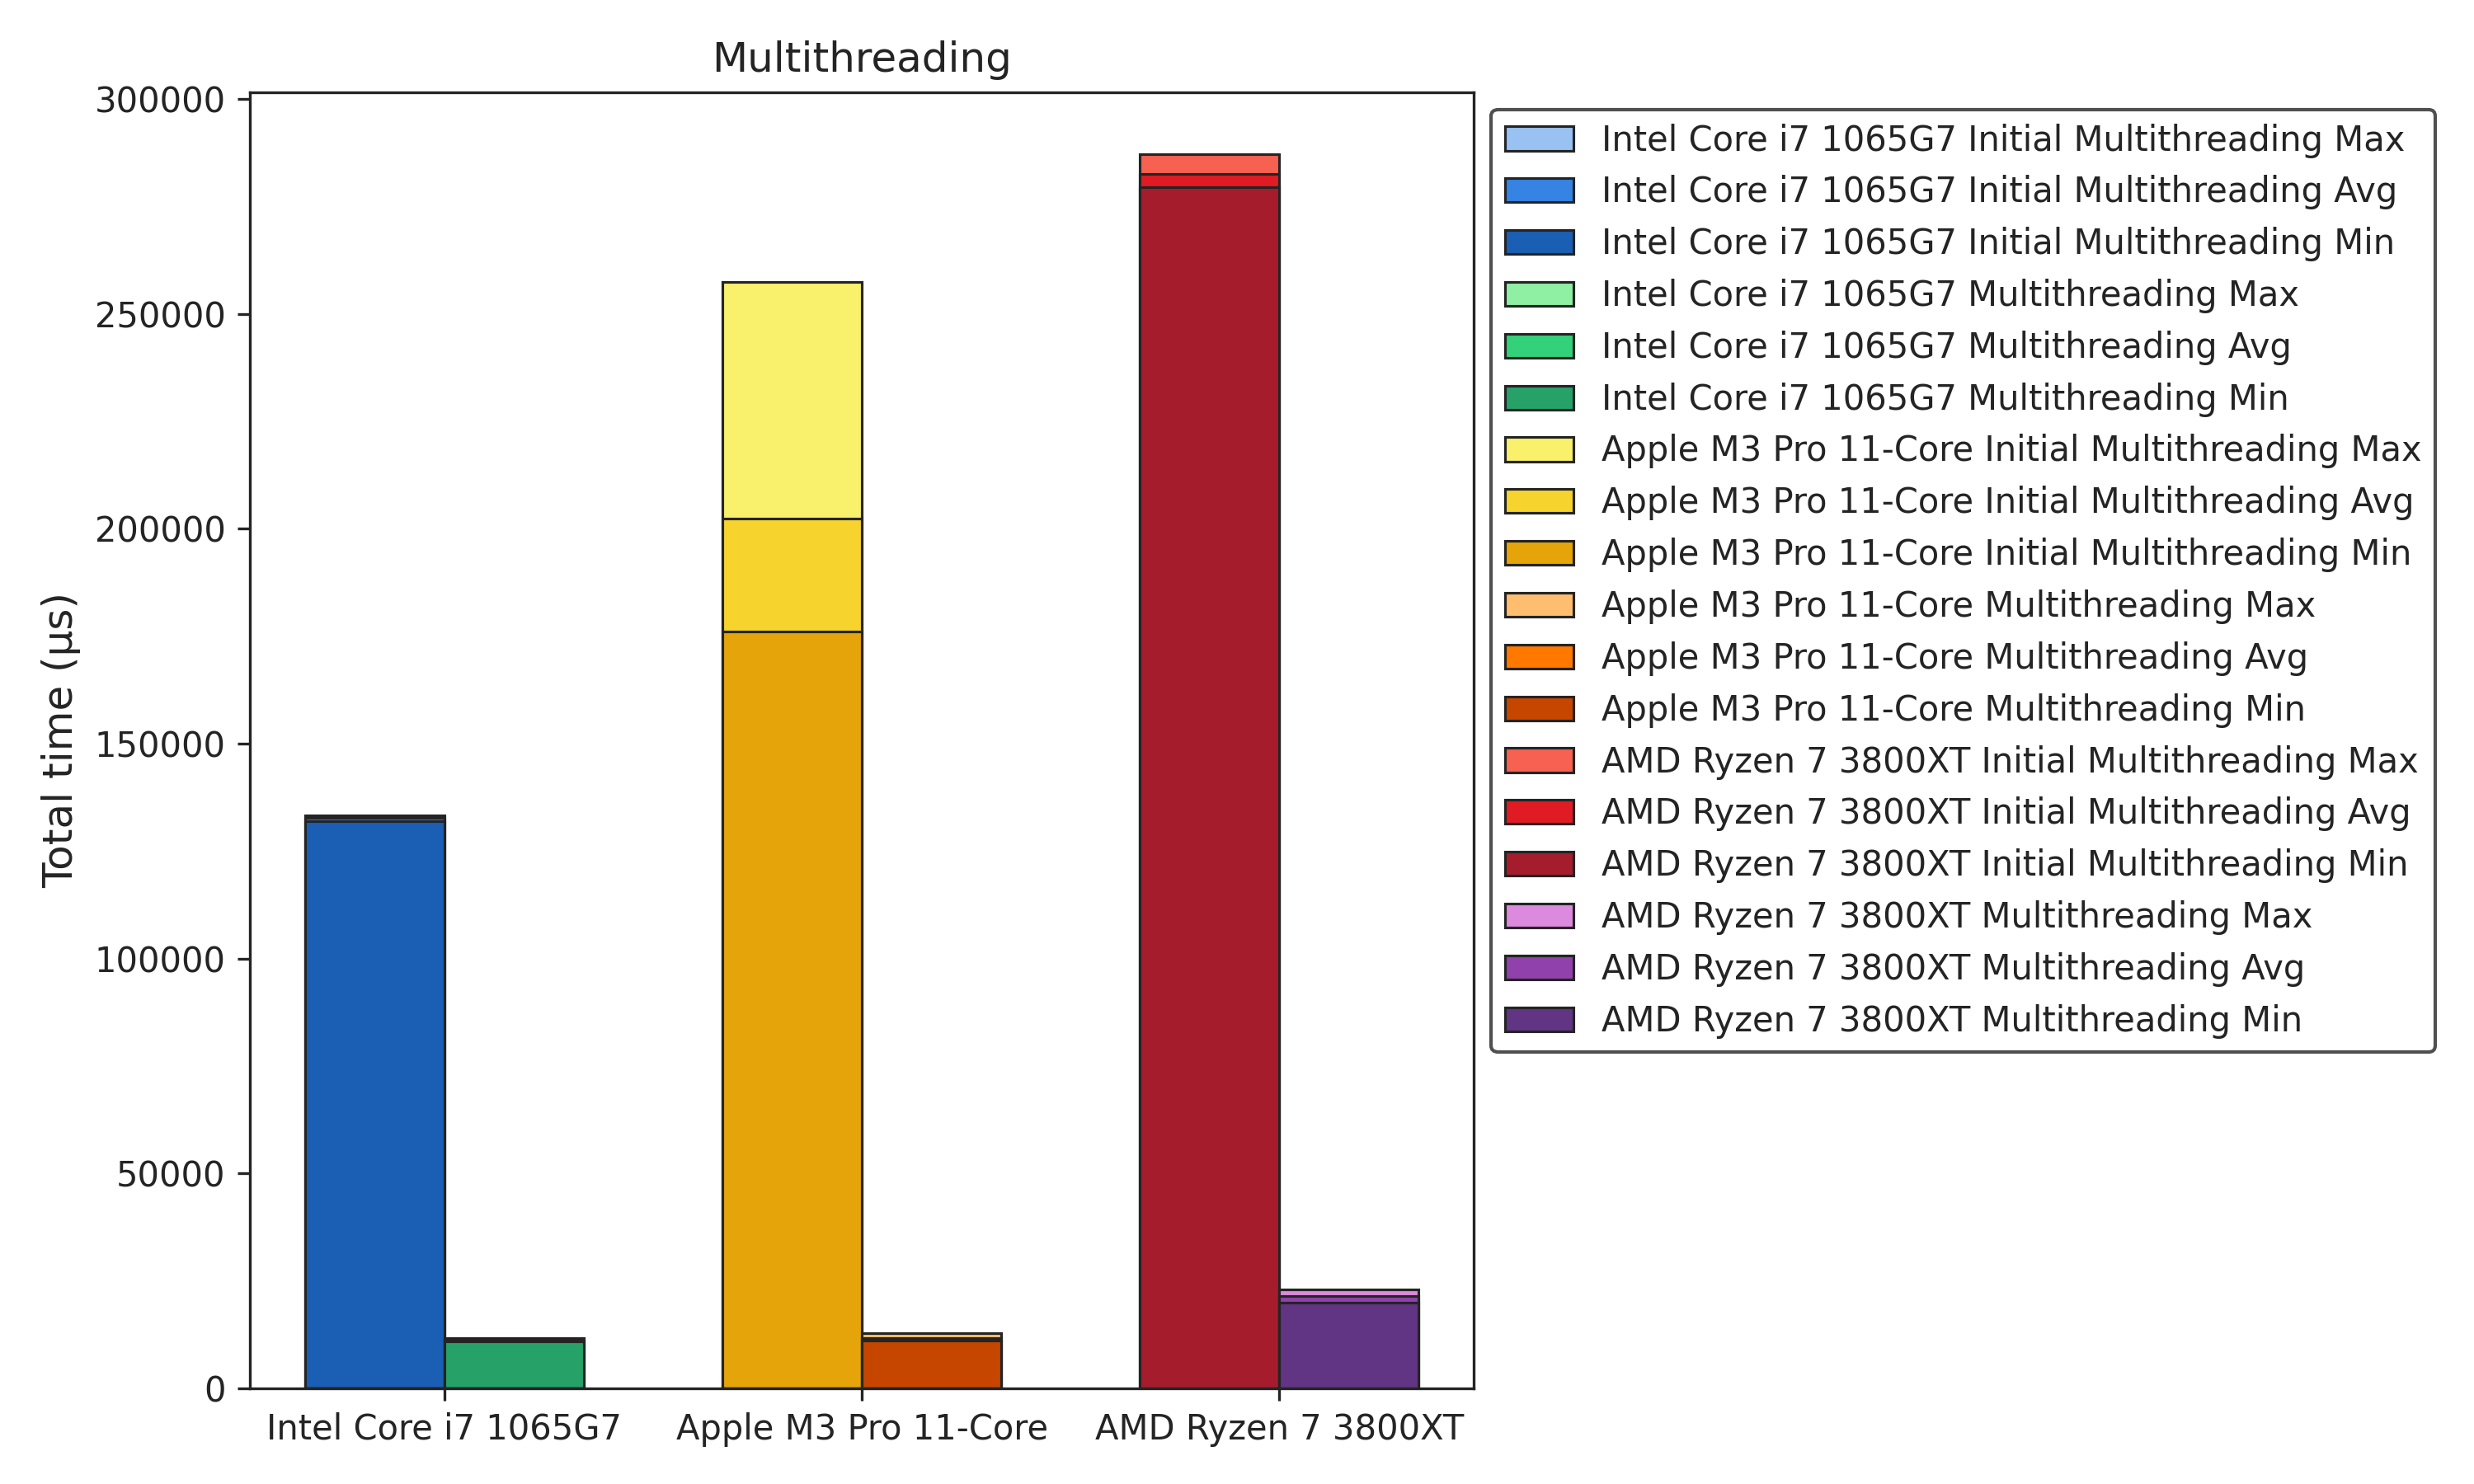
\includegraphics[width=\linewidth]{Graphs/Multithreading.png}
  \caption{On the MNIST dataset}
 \label{fig:multithreading_mnist}
\end{subfigure}%
\begin{subfigure}{.5\textwidth}
  \centering
  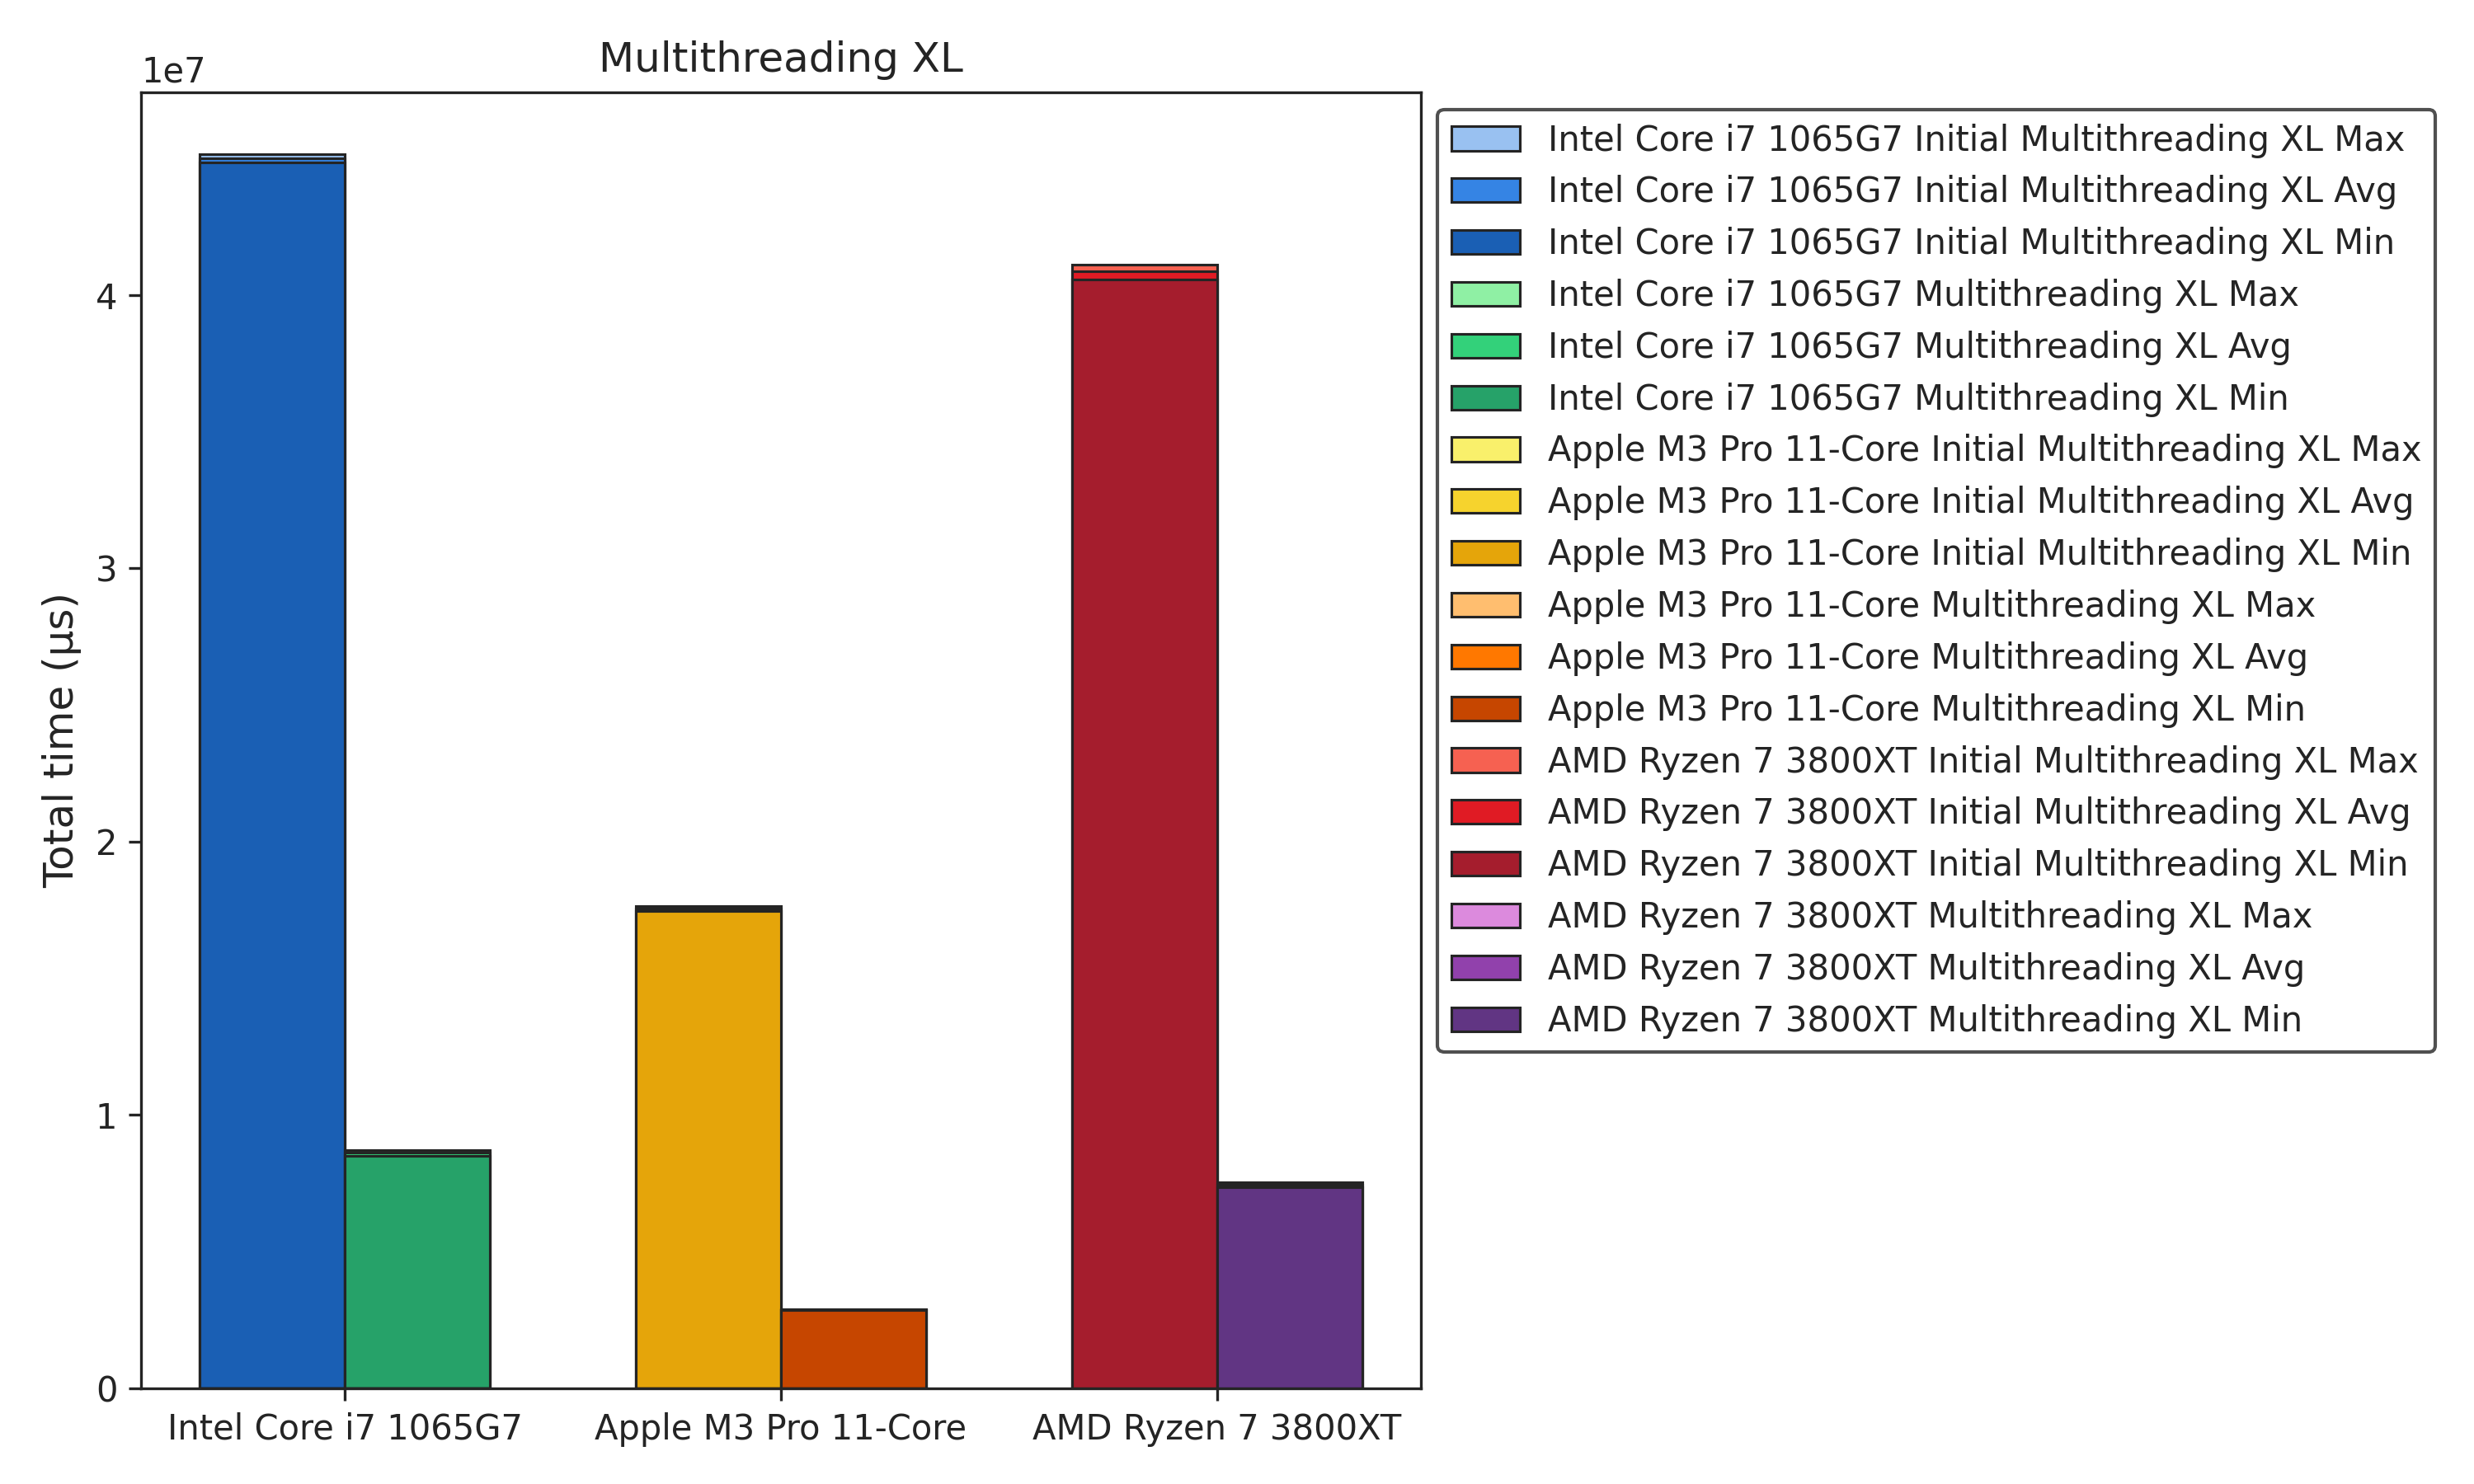
\includegraphics[width=\linewidth]{Graphs/Multithreading XL.png}
  \caption{On the synthetic XL dataset}
 \label{fig:multithreading_xl}
\end{subfigure}
\caption{Performance benchmarks of the optimized multithreading implementation}
\label{fig:multithreading}
\end{figure}
\begin{table}[htb!]
\centering
\caption{Optimized Multithreading Implementation\label{tab:multithreading}}
\begin{tabular}{p{5cm} p{2cm} p{2cm} p{2cm} p{2cm}}
\hline
Benchmark Name & Minimum Value ($\mu$s) & Average Value ($\mu$s) & Maximum Value ($\mu$s) & Standard Deviation \\
\hline
Intel Core i7-1065G7 \\
\hspace{0.5cm}Initial Multithreading & 131866.0 & 132756.0 & 133229.0 & 366.1 \\
\hspace{0.5cm}Multithreading & 10851.0 & 11205.8 & 11643.0 & 231.2 \\
Apple M3 Pro 11-Core \\
\hspace{0.5cm}Initial Multithreading & 176040.0 & 202359.7 & 257459.0 & 21555.6 \\
\hspace{0.5cm}Multithreading & 11155.0 & 11707.3 & 12729.0 & 598.2 \\
AMD Ryzen 7 3800XT \\
\hspace{0.5cm}Initial Multithreading & 279513.0 & 282589.0 & 287196.0 & 2643.1 \\
\hspace{0.5cm}Multithreading & 19826.0 & 21530.2 & 22967.0 & 824.8 \\
\hline
Intel Core i7-1065G7 \\
\hspace{0.5cm}Initial Multithreading XL & 44870433.0 & 45002714.3 & 45163577.0 & 102509.7 \\
\hspace{0.5cm}Multithreading XL & 8500620.0 & 8636423.7 & 8721267.0 & 75104.0 \\
Apple M3 Pro 11-Core \\
\hspace{0.5cm}Initial Multithreading XL & 17466123.0 & 17567938.9 & 17641156.0 & 61687.5 \\
\hspace{0.5cm}Multithreading XL & 2848506.0 & 2867258.2 & 2903430.0 & 19278.1 \\
AMD Ryzen 7 3800XT \\
\hspace{0.5cm}Initial Multithreading XL & 40573406.0 & 40867988.9 & 41106348.0 & 185968.0 \\
\hspace{0.5cm}Multithreading XL & 7352356.0 & 7438704.9 & 7552378.0 & 63658.1 \\
\hline
\end{tabular}
\end{table}
\FloatBarrier

Achieving 92.8\% on the MNIST dataset and 81.7\% on the synthetic XL dataset represents truly remarkable improvements, surpassing even our highest expectations. With this progress, we are now very close to the theoretical maximum possible speedup for multithreading, which is the number of available cores. Although we are comparing the initial multithreading implementation with the optimized version, it is interesting to note that, counterintuitively, the performance degradation in the average across all CPUs on the MNIST dataset is only 457.7\% in the initial implementation, which is significantly less than the 92.8\% improvement observed here. This suggests that performance has significantly increased compared to the naive implementation, as we will discuss in a later chapter. This is also evident when looking at the synthetic XL dataset, where performance was already improved in the initial multithreading implementation, but was further optimized by an additional 81.7\% on average across all CPUs.

Overall, we have successfully met all of our objectives. The total time has decreased significantly, leading to a corresponding rise in performance. Resource usage has increased from about 20\% on a single core to 100\% across all cores. While there is a possibility that we are pushing the CPUs beyond their limits, we are undoubtedly extracting the maximum possible performance from the hardware. Scalability was already improved in the initial multithreading implementation. However, in the optimized version, the difference between the increase in problem size and the rise in total time has now been minimized.
\subsection{OpenMP}\label{sec:openmp}
\subsubsection{Overview}\label{sec:openmp_overview}
OpenMP (Open Multi-Processing) is a widely used API that provides parallel programming support for languages like C and C++ on several CPU- and GPU-architectures. It enables developers to write parallel programs without manually facing the difficulties of multithreading, thereby simplifying the development of parallel applications and allowing minimal code changes while taking full advantage of multi-core processors.

It utilizes pragmas (compiler directives) to define parallel regions within a program, instructing the compiler to parallelize specific code segments. For instance, the \texttt{\#pragma omp for} can parallelize a loop, thereby reducing the complexity typically associated with parallel programming. It is designed to efficiently utilize modern multi-core processors. It facilitates dynamic load balancing, wherein work is apportioned across cores based on their current load, leading to enhanced resource utilization and reduced execution time. It is noteworthy that the majority of the work is obscured from the developer and is managed on the compiler side. Consequently, there is limited transparency and flexibility.\footnote{Introduction to OpenMP: \url{https://blog.rwth-aachen.de/hpc_import_20210107/attachments/35947076/36143199.pdf} (accessed April 18, 2025).}

\begin{figure}[htb!]
\centering
\begin{subfigure}{.5\textwidth}
  \centering
  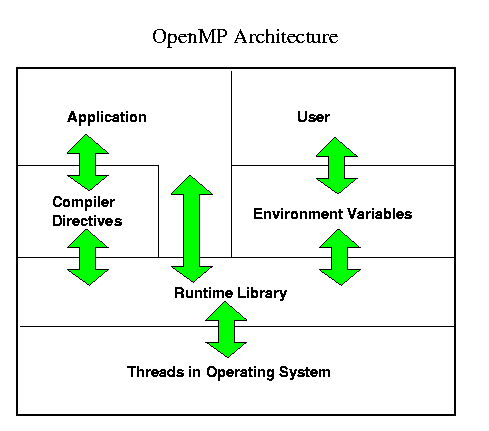
\includegraphics[width=\linewidth]{OpenMP/OpenMP Architecture.png}
  \caption{\label{fig:openmp_architecture}}
\end{subfigure}%
\begin{subfigure}{.5\textwidth}
  \centering
  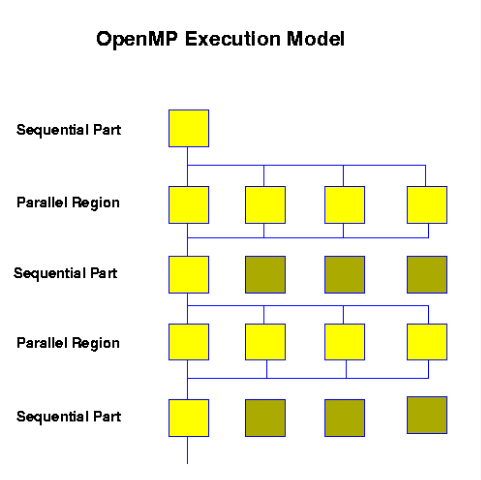
\includegraphics[width=\linewidth]{OpenMP/OpenMP Execution Model.png}
  \caption{\label{fig:openmp_execution}}
\end{subfigure}
\caption{Structural Overview of OpenMP\label{fig:openmp_overview}\footnote{OpenMP - shared memory and device parallelism: \url{https://doku.lrz.de/openmp-shared-memory-and-device-parallelism-11481693.html} (accessed April 18, 2025).}}
\end{figure}

The Figure~\ref{fig:openmp_overview} above outlines the two primary mechanisms through which programmers interface with OpenMP’s implicit parallel execution layer: compiler directives and environment variables such as \texttt{OMP\_NUM\_THREADS}, which sets the number of threads allocated to parallel regions. Additional environment variables are detailed in the OpenMP documentation.\footnote{Environment Variables: \url{https://www.openmp.org/spec-html/5.0/openmpch6.html} (accessed April 18, 2025).} These directives and variables are ultimately translated into runtime library calls that orchestrate parallelism. 

OpenMP supports multiple parallelization strategies, including loop, task, and data parallelism, each of which is particularly well-suited for distinct types of problems. Loop parallelism involves the division of iterations of a loop across multiple threads, while task parallelism involves the assignment of independent tasks to different threads. Data parallelism, on the other hand, enables the execution of operations on large data sets concurrently. Furthermore, OpenMP provides task scheduling options, such as static, dynamic, and guided, allowing for a high degree of control over the distribution of work among threads to optimize performance.

OpenMP supports a large set of compiler directives that are embedded directly in the code. The most common pragmas include \texttt{\#pragma omp parallel}, \texttt{\#pragma omp for}, and \texttt{\#pragma omp section}, which control the parallelization of loops, sections of code, and task execution.

Additionally, OpenMP offers library routines for managing parallel tasks, such as setting the number of threads with \texttt{omp\_set\_num\_threads()} or retrieving the number of available threads (\texttt{omp\_get\_num\_threads()}). Moreover, environment variables like \texttt{OMP\_NUM\_THREADS} allow users to set the number of threads at runtime.

For the sake of completeness, we should mention another feature of OpenMP called offload targets, which allow computations to be executed on other devices such as GPUs, additional processors, or other specialized hardware. This is particularly useful for calculations that can be performed more quickly on the GPU, such as matrix multiplications. In order to use this feature, the compiler, in our case either GCC or Clang, must be recompiled accordingly. However, both the Arm chip and the presented Intel chip do not support offload targets, which is why we did not pursue this approach further.\footnote{Intro to GPU Programming with the OpenMP API: \url{https://www.openmp.org/wp-content/uploads/2021-10-20-Webinar-OpenMP-Offload-Programming-Introduction.pdf} (accessed April 19, 2025).}
\subsubsection{Implementation}
To utilize OpenMP for our project, we have enabled different compiler flags depending on the architecture (illustrated here for Clang).

\begin{itemize}
    \item AMD: \texttt{-Xcompiler -fopenmp}
    \item Arm: \texttt{-Xclang -fopenmp}
    \item Intel: \texttt{-Xcompiler -qopenmp}
\end{itemize}

Through these compiler flags, the pragmas are recognized and appropriately interpreted by the compiler. No further intervention by the developer is required at this point.

As an example, consider the function~\ref{lst:add-function}, which adds two matrices:

\newpage
\begin{lstlisting}[
    caption={Excerpt of add-function},
    label={lst:add-function},
    language=C++,
    numbers=left,
    numbersep=10pt,
    basicstyle=\fontsize{10}{10}\selectfont,
    breaklines=true,
    postbreak=\mbox{\textcolor{red}{$\hookrightarrow$}\space},
    frame=single,
]
/*
* @param a: Input-Matrix a
* @param b: Input-Matrix b
* @param c: Output-Matrix c
* @param mt: Multithreading object
* @return: Matrix c as a result of a + b
*/
matrix *add(void *a, void *b, matrix *c, mt *instance) {
#pragma omp parallel for collapse(2)
    for(int i = 0; i < c->x; i++) {
        for(int j = 0; j < c->y; j++) {
            // ...
       }
    }
}
\end{lstlisting}

Attention is drawn to the pragma in line 9. This pragma must be interpreted in two parts. \texttt{\#pragma omp parallel for} instructs the compiler to execute a loop in parallel by distributing it across multiple threads. It ensures that the loop immediately following it is parallelized. The second part, \texttt{collapse(2)}, indicates that two loops (the two outer loops) are collapsed and treated as a single loop. OpenMP can then divide the iterations of these two loops among the available threads.

We have implemented this pragma for all functions used in \texttt{tf.cpp} and adapted it accordingly based on the number of for-loops.

While OpenMP is often praised as a versatile "Swiss Army knife" for parallel programming, our analysis reveals inherent limitations in its ability to automatically optimize code. A notable example arises during the compilation of the convolutional function~\ref{lst:conv2d-warning}, where the compiler generates the warning:
\begin{lstlisting}[
    caption={OpenMP Warning of conv2d()},
    label={lst:conv2d-warning},
    language=Bash,
    numbers=left,
    numbersep=10pt,
    basicstyle=\fontsize{10}{10}\selectfont,
    breaklines=true,
    postbreak=\mbox{\textcolor{red}{$\hookrightarrow$}\space},
    frame=single,
]
warning: loop not vectorized: the optimizer was unable
to perform the requested transformation; 
the transformation might be disabled or specified as
part of an unsupported transformation ordering 
[-Wpass-failed=transform-warning]
\end{lstlisting}
This warning specifically highlights OpenMP's inability to vectorize a critical loop within \texttt{conv2d()} — a common operation in computational kernels. While OpenMP simplifies task parallelism through pragma directives, this instance underscores its suboptimal handling of data-level parallelism. The failure to auto-vectorize suggests either (1) unresolved loop-carried dependencies, (2) non-contiguous memory access patterns, or (3) insufficient structural hints for the compiler to apply SIMD optimizations.
\subsubsection{Performance Benchmarks}
The benchmark results are shown in Figure~\ref{fig:openmp}, with the corresponding values listed in Table~\ref{tab:openmp}. The average performance of all CPUs on the MNIST dataset decreases by 219.89\%. The average performance of the Intel Core i7-1065G7 decreases by 286.4\%, the Apple M3 Pro 11-Core decreases by 271.3\%, and the AMD Ryzen 7 3800XT decreases by 157.4\%. The average performance of all CPUs on the synthetic XL dataset decreases by 467.5\%. The Intel Core i7-1065G7 decreases by 495.3\%, the Apple M3 Pro 11-Core decreases by 369.2\%, and the AMD Ryzen 7 3800XT decreases by 369.2\%. 
\begin{figure}[htb!]
\centering
\begin{subfigure}{.5\textwidth}
  \centering
  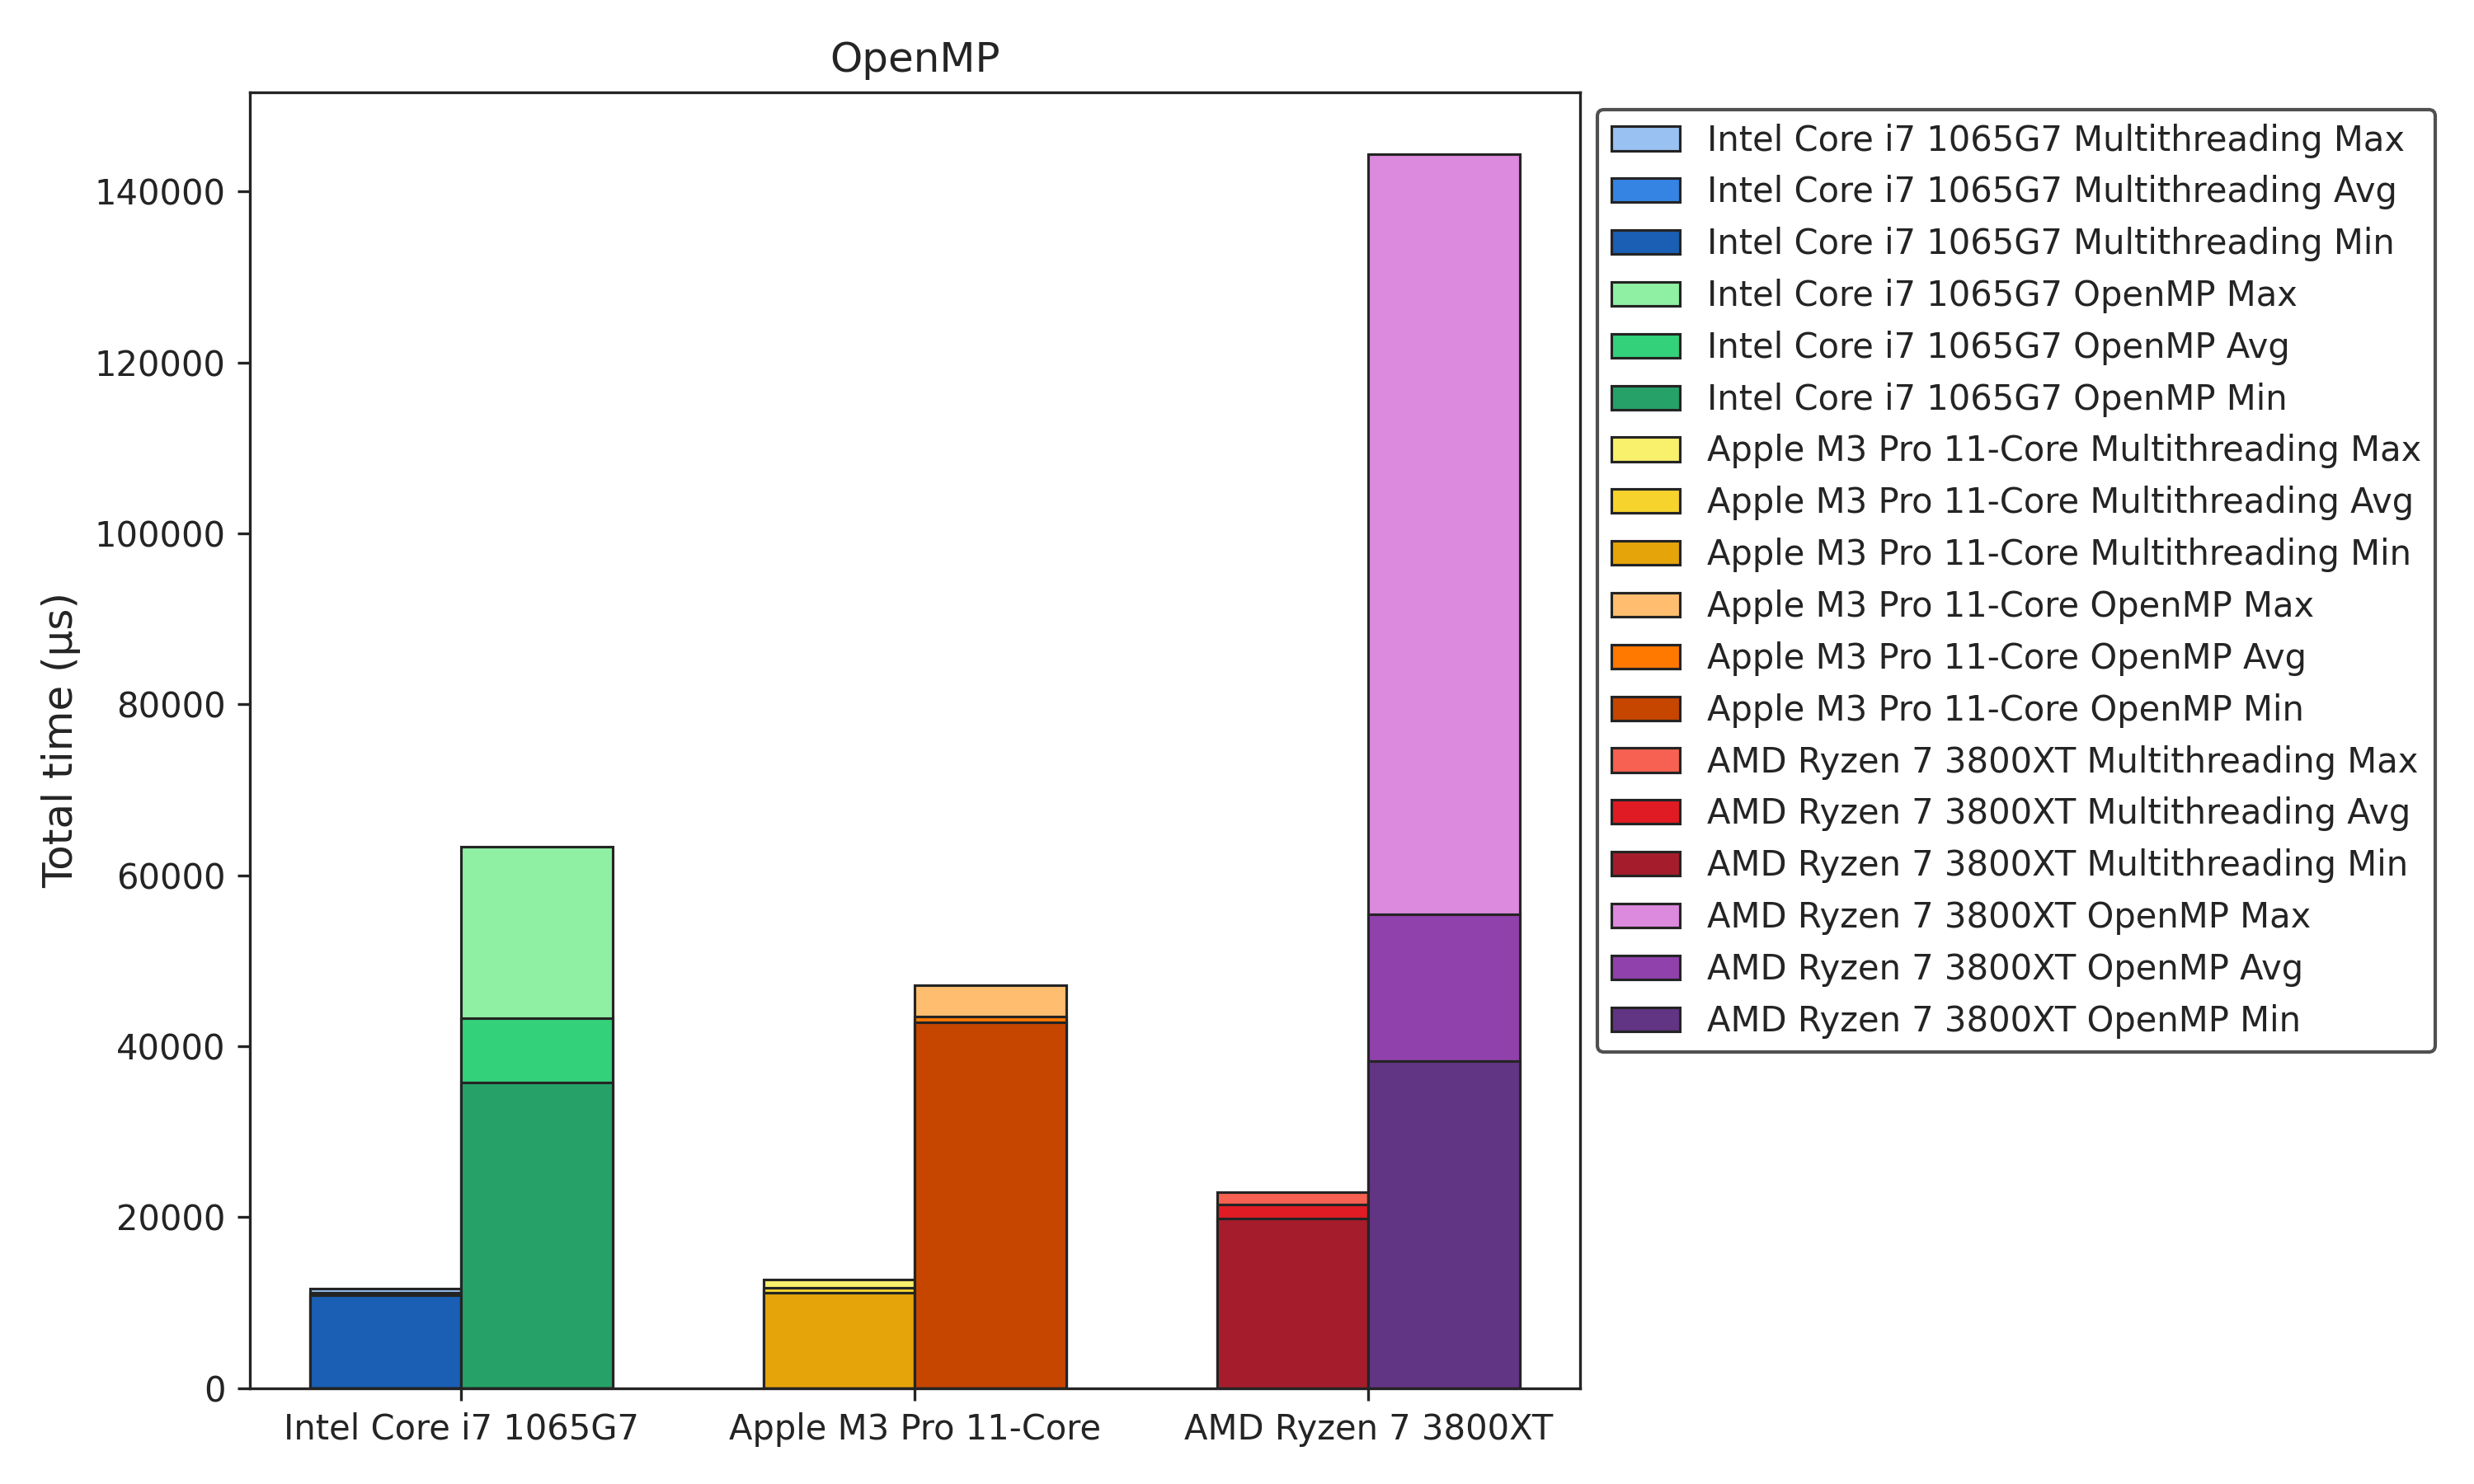
\includegraphics[width=\linewidth]{Graphs/OpenMP.png}
  \caption{On the MNIST dataset}
 \label{fig:openmp_mnist}
\end{subfigure}%
\begin{subfigure}{.5\textwidth}
  \centering
  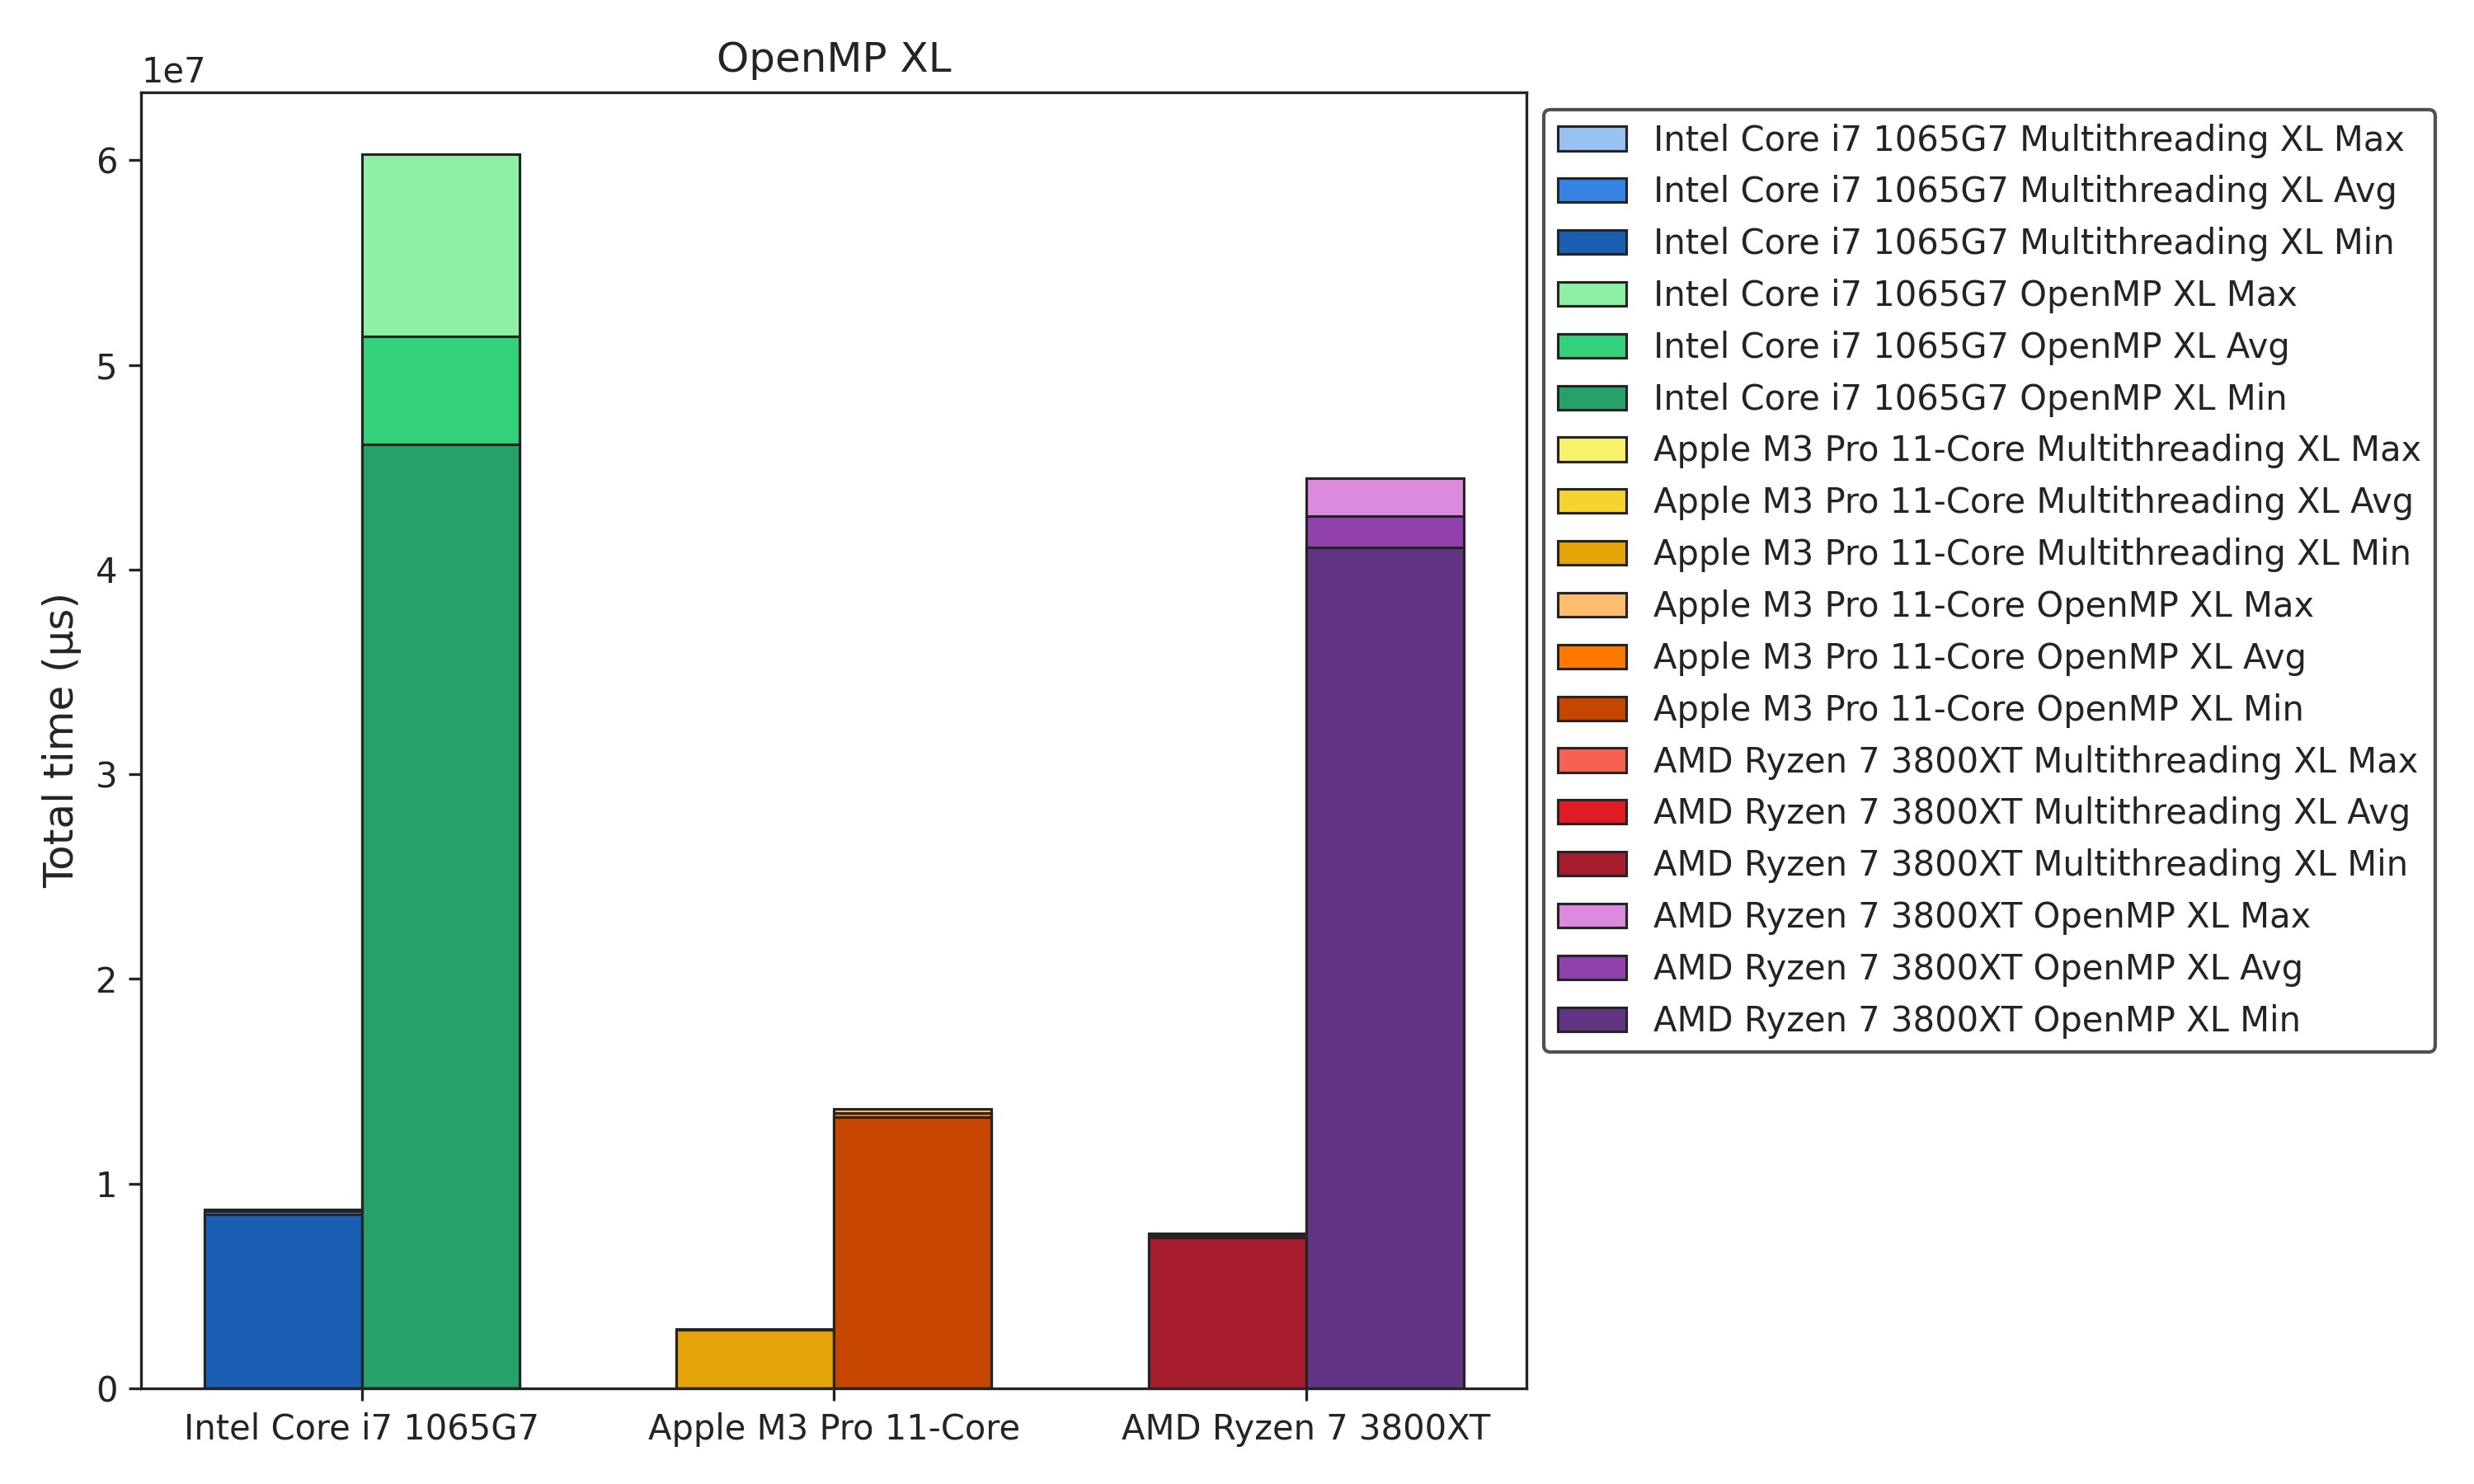
\includegraphics[width=\linewidth]{Graphs/OpenMP XL.png}
  \caption{On the synthetic XL dataset}
 \label{fig:openmp_xl}
\end{subfigure}
\caption{Performance benchmarks of OpenMP}
\label{fig:openmp}
\end{figure}
\begin{table}[htb!]
\centering

\caption{OpenMP\label{tab:openmp}}
\begin{tabular}{p{5cm} p{2cm} p{2cm} p{2cm} p{2cm}}
\hline
Benchmark Name & Minimum Value ($\mu$s) & Average Value ($\mu$s) & Maximum Value ($\mu$s) & Standard Deviation \\
\hline
Intel Core i7-1065G7 \\
\hspace{0.5cm}Multithreading & 10851.0 & 11205.8 & 11643.0 & 231.2 \\
\hspace{0.5cm}OpenMP & 35733.0 & 43297.5 & 63330.0 & 7658.0 \\
Apple M3 Pro 11-Core \\
\hspace{0.5cm}Multithreading & 11155.0 & 11707.3 & 12729.0 & 598.2 \\
\hspace{0.5cm}OpenMP & 42809.0 & 43465.5 & 47122.0 & 1235.9 \\
AMD Ryzen 7 3800XT \\
\hspace{0.5cm}Multithreading & 19826.0 & 21530.2 & 22967.0 & 824.8 \\
\hspace{0.5cm}OpenMP & 38261.0 & 55426.5 & 144388.0 & 31422.4 \\
\hline
Intel Core i7-1065G7 \\
\hspace{0.5cm}Multithreading XL & 8500620.0 & 8636423.7 & 8721267.0 & 75104.0 \\
\hspace{0.5cm}OpenMP XL & 46136509.0 & 51416232.8 & 60306735.0 & 4473869.3 \\
Apple M3 Pro 11-Core \\
\hspace{0.5cm}Multithreading XL & 2848506.0 & 2867258.2 & 2903430.0 & 19278.1 \\
\hspace{0.5cm}OpenMP XL & 13228160.0 & 13454528.5 & 13668817.0 & 179126.7 \\
AMD Ryzen 7 3800XT \\
\hspace{0.5cm}Multithreading XL & 7352356.0 & 7438704.9 & 7552378.0 & 63658.1 \\
\hspace{0.5cm}OpenMP XL & 41100356.0 & 42629449.5 & 44471702.0 & 1254546.1 \\
\hline
\end{tabular}
\end{table}
\FloatBarrier

OpenMP yields significantly poorer results compared to the multithreading approach described in \autoref{sec:multithreading}. A potential reason for this is that OpenMP destroys threads once they exit a parallel region (see also Figure~\ref{fig:openmp_execution}). This introduces additional overhead, which can negatively impact performance.
One possible improvement on the OpenMP side could be achieved by adjusting the scheduling strategy. By default, OpenMP uses a static scheduling approach; however, this can be modified dynamically using the directive \texttt{\#pragma omp for schedule(dynamic, chunk\_size)}. Although this approach was not evaluated in the scope of this work, it presents a promising foundation for future research.
It should also be noted that OpenMP heavily relies on compiler optimizations. Therefore, the compiler flag \texttt{-O3} should be applied — as was the case in the benchmarks presented here.
\subsection{Compiler and Build Tools}
\subsubsection{GCC and Clang}\label{subsec:gcc-and-clang}
During the implementation phase, various compilers were used, starting with GCC and ultimately transitioning to Clang. This chapter aims to briefly illustrate the differences between these two compilers. GCC, developed as part of the GNU Project, is widely regarded as the gold standard in compiler technology. In contrast, Clang was initiated by Apple and later integrated into the LLVM project. While GCC is well-suited for monolithic architectures, Clang is considered a more modern and modular alternative.

Clang is known for its clear and detailed error messages, whereas GCC provides comparatively more concise diagnostics. On the other hand, GCC tends to offer slightly better compiler optimizations. Notably, Clang includes integrated tools such as clang-tidy and clang-format, which facilitate refactoring and code quality assurance. Given that this framework was developed over the course of several months with continuously evolving features, refactoring was a constant and essential aspect throughout the development process.

Since our framework supports multiple architectures and runs on Arm, AMD, and Intel platforms, we opted for a compiler that provides robust support on macOS. In this context, Clang proved to be the most reliable choice. While development using GCC would have been feasible, it would likely have slowed down the process due to the need for additional workarounds. In contrast, Clang functioned seamlessly across all target devices without further limitations.

Furthermore, both GCC and Clang support OpenMP as well as native threads, which is advantageous for the framework presented here. With regard to the aforementioned (see \ref{sec:openmp_overview}) OpenMP offload targets, the Clang compiler was recompiled multiple times on both the Intel CPU and the Apple Silicon chip. However, these efforts were unsuccessful, and it was concluded that neither of these devices provides support for offloading targets.

Finally, the two primary debugging options are briefly introduced. On one hand, GCC utilizes GDB, which is stable and well-optimized. On the other hand, Clang employs LLDB, which is part of the LLVM project and offers faster startup times.\footnote{GCC vs. Clang: \url{https://www.incredibuild.com/blog/gcc-vs-clang-battle-of-the-behemoths} (accessed April 18, 2025).}$^{,}$\footnote{GCC vs. Clang/LLVM: \url{https://alibabatech.medium.com/gcc-vs-clang-llvm-an-in-depth-comparison-of-c-c-compilers-899ede2be378} (accessed April 18, 2025).}

The compiler optimization flags and most of the features available in GCC are also accessible in Clang. In summary, the use of Clang has not resulted in any performance decrease.
\subsubsection{Intel C++ Compiler}\label{subsec:intel-c++-compiler}
After choosing Clang primarily for macOS compatibility and observing no significant performance difference compared to GCC, we now aim to compare it with a more specialized compiler, from which we expect performance improvements without needing to modify a single line of code. We select the Intel oneAPI DPC++/C++ Compiler (ICPX), formerly known as the Intel C++ Compiler (ICPC). This compiler offers several key advantages: it delivers excellent performance through industry-leading Intel compiler technology, generates optimized binary host and accelerator code, leverages Intel oneAPI's optimized performance and threading libraries, integrates seamlessly with popular third-party compilers, development environments, and operating systems, supports the latest standards such as C++23 and OpenMP for CPU and GPU offload, and uses LLVM sanitizers to detect bugs early in the development cycle. This ensures that C++ and OpenMP code is more reliable, secure, and easier to maintain across both CPU and GPU platforms.\footnote{Intel oneAPI DPC++/C++ Compiler: \url{https://www.intel.com/content/www/us/en/developer/tools/oneapi/dpc-compiler.html} (accessed April 14, 2025).}

Although the compiler is specifically developed and optimized for Intel CPUs, we anticipate similar performance improvements on AMD CPUs, given that they share the same x86 architecture. However, Arm processors, such as Apple Silicon, and macOS in general, are not supported and are thus excluded from the comparison.

The command-line interface (CLI) of ICPX behaves differently from Clang's, requiring us to significantly adjust the Makefile, though we still make no changes to the actual code. Both compilers are used with maximum optimization (-O3), and accuracy is verified to ensure that no erroneous optimizations occur.

Now, we compare Clang and ICPX based on the performance of the naive implementation and the OpenMP implementation.

The benchmark results based on the naive implementation are shown in Figure~\ref{fig:icpx}, with the corresponding values listed in Table~\ref{tab:icpx}. The average performance of all CPUs on the MNIST dataset improves by 55.8\%. The average performance of the Intel Core i7-1065G7 improves by 57.6\% and the AMD Ryzen 7 3800XT improves by 53.9\%. The average performance of all CPUs on the synthetic XL dataset improves by 57.8\%. The Intel Core i7-1065G7 improves by 58.9\% and the AMD Ryzen 7 3800XT improves by 56.7\%.
\begin{figure}[htb!]
\centering
\begin{subfigure}{.5\textwidth}
  \centering
  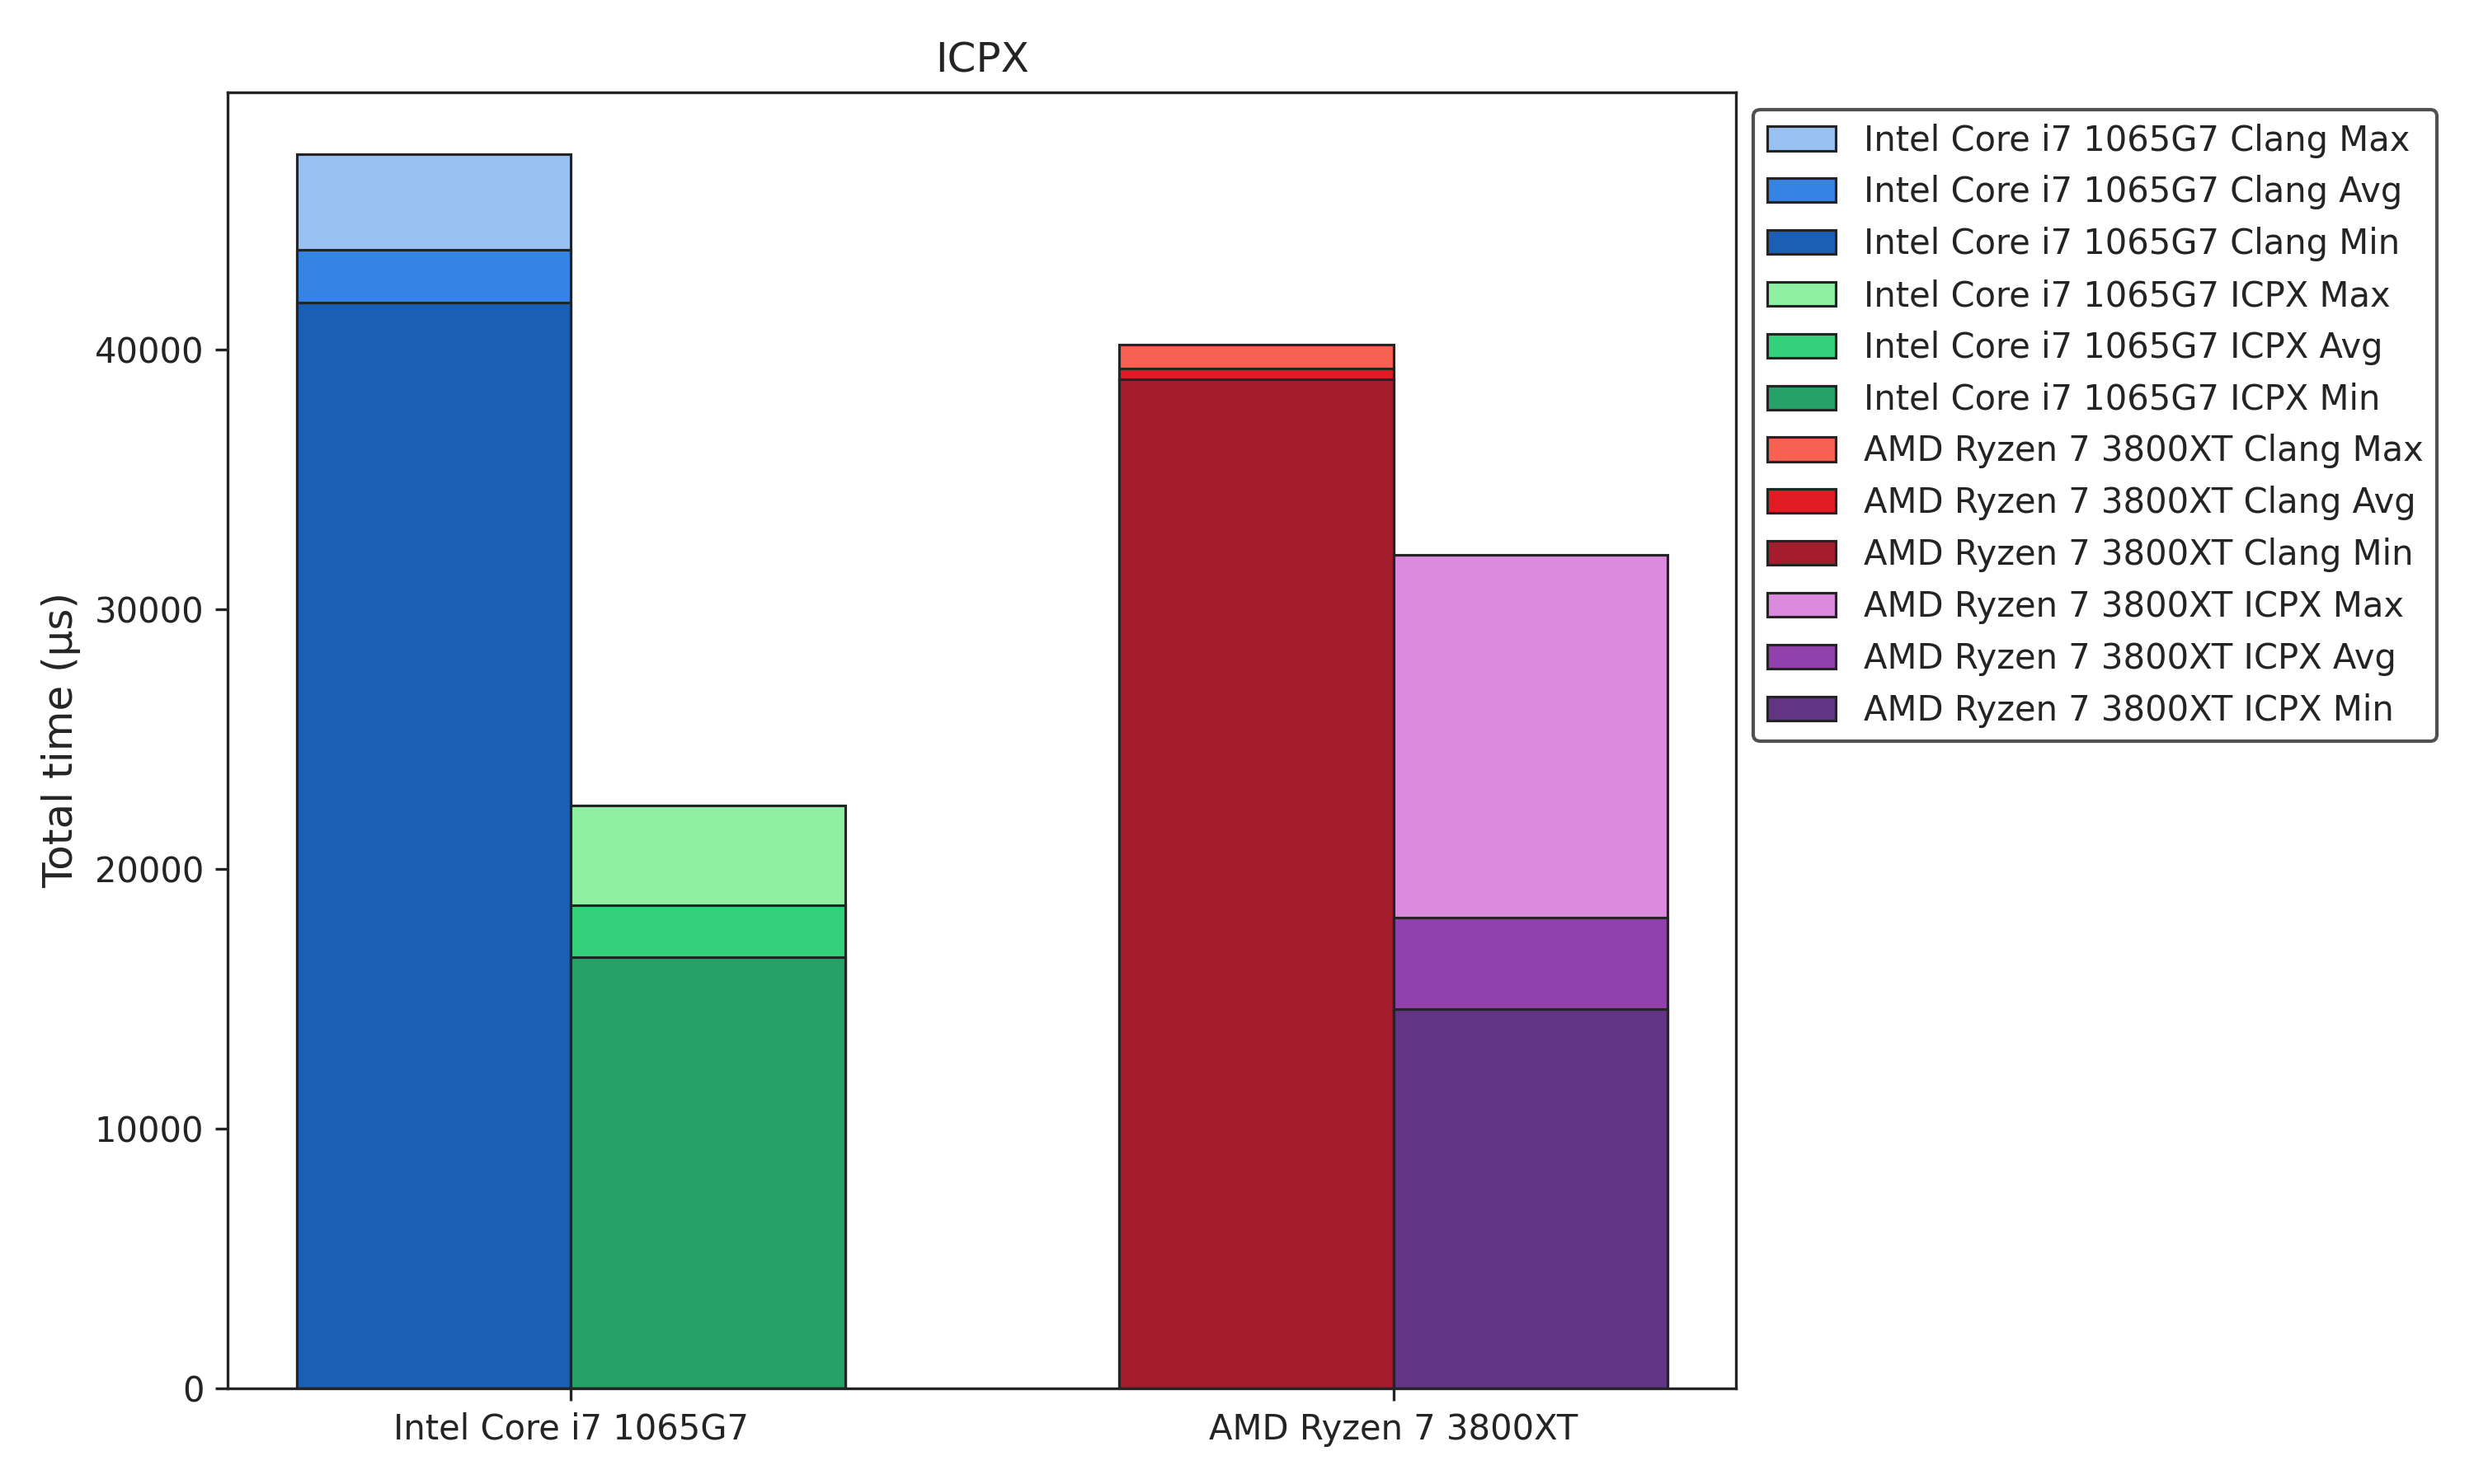
\includegraphics[width=\linewidth]{Graphs/ICPX.png}
  \caption{On the MNIST dataset}
 \label{fig:icpx_mnist}
\end{subfigure}%
\begin{subfigure}{.5\textwidth}
  \centering
  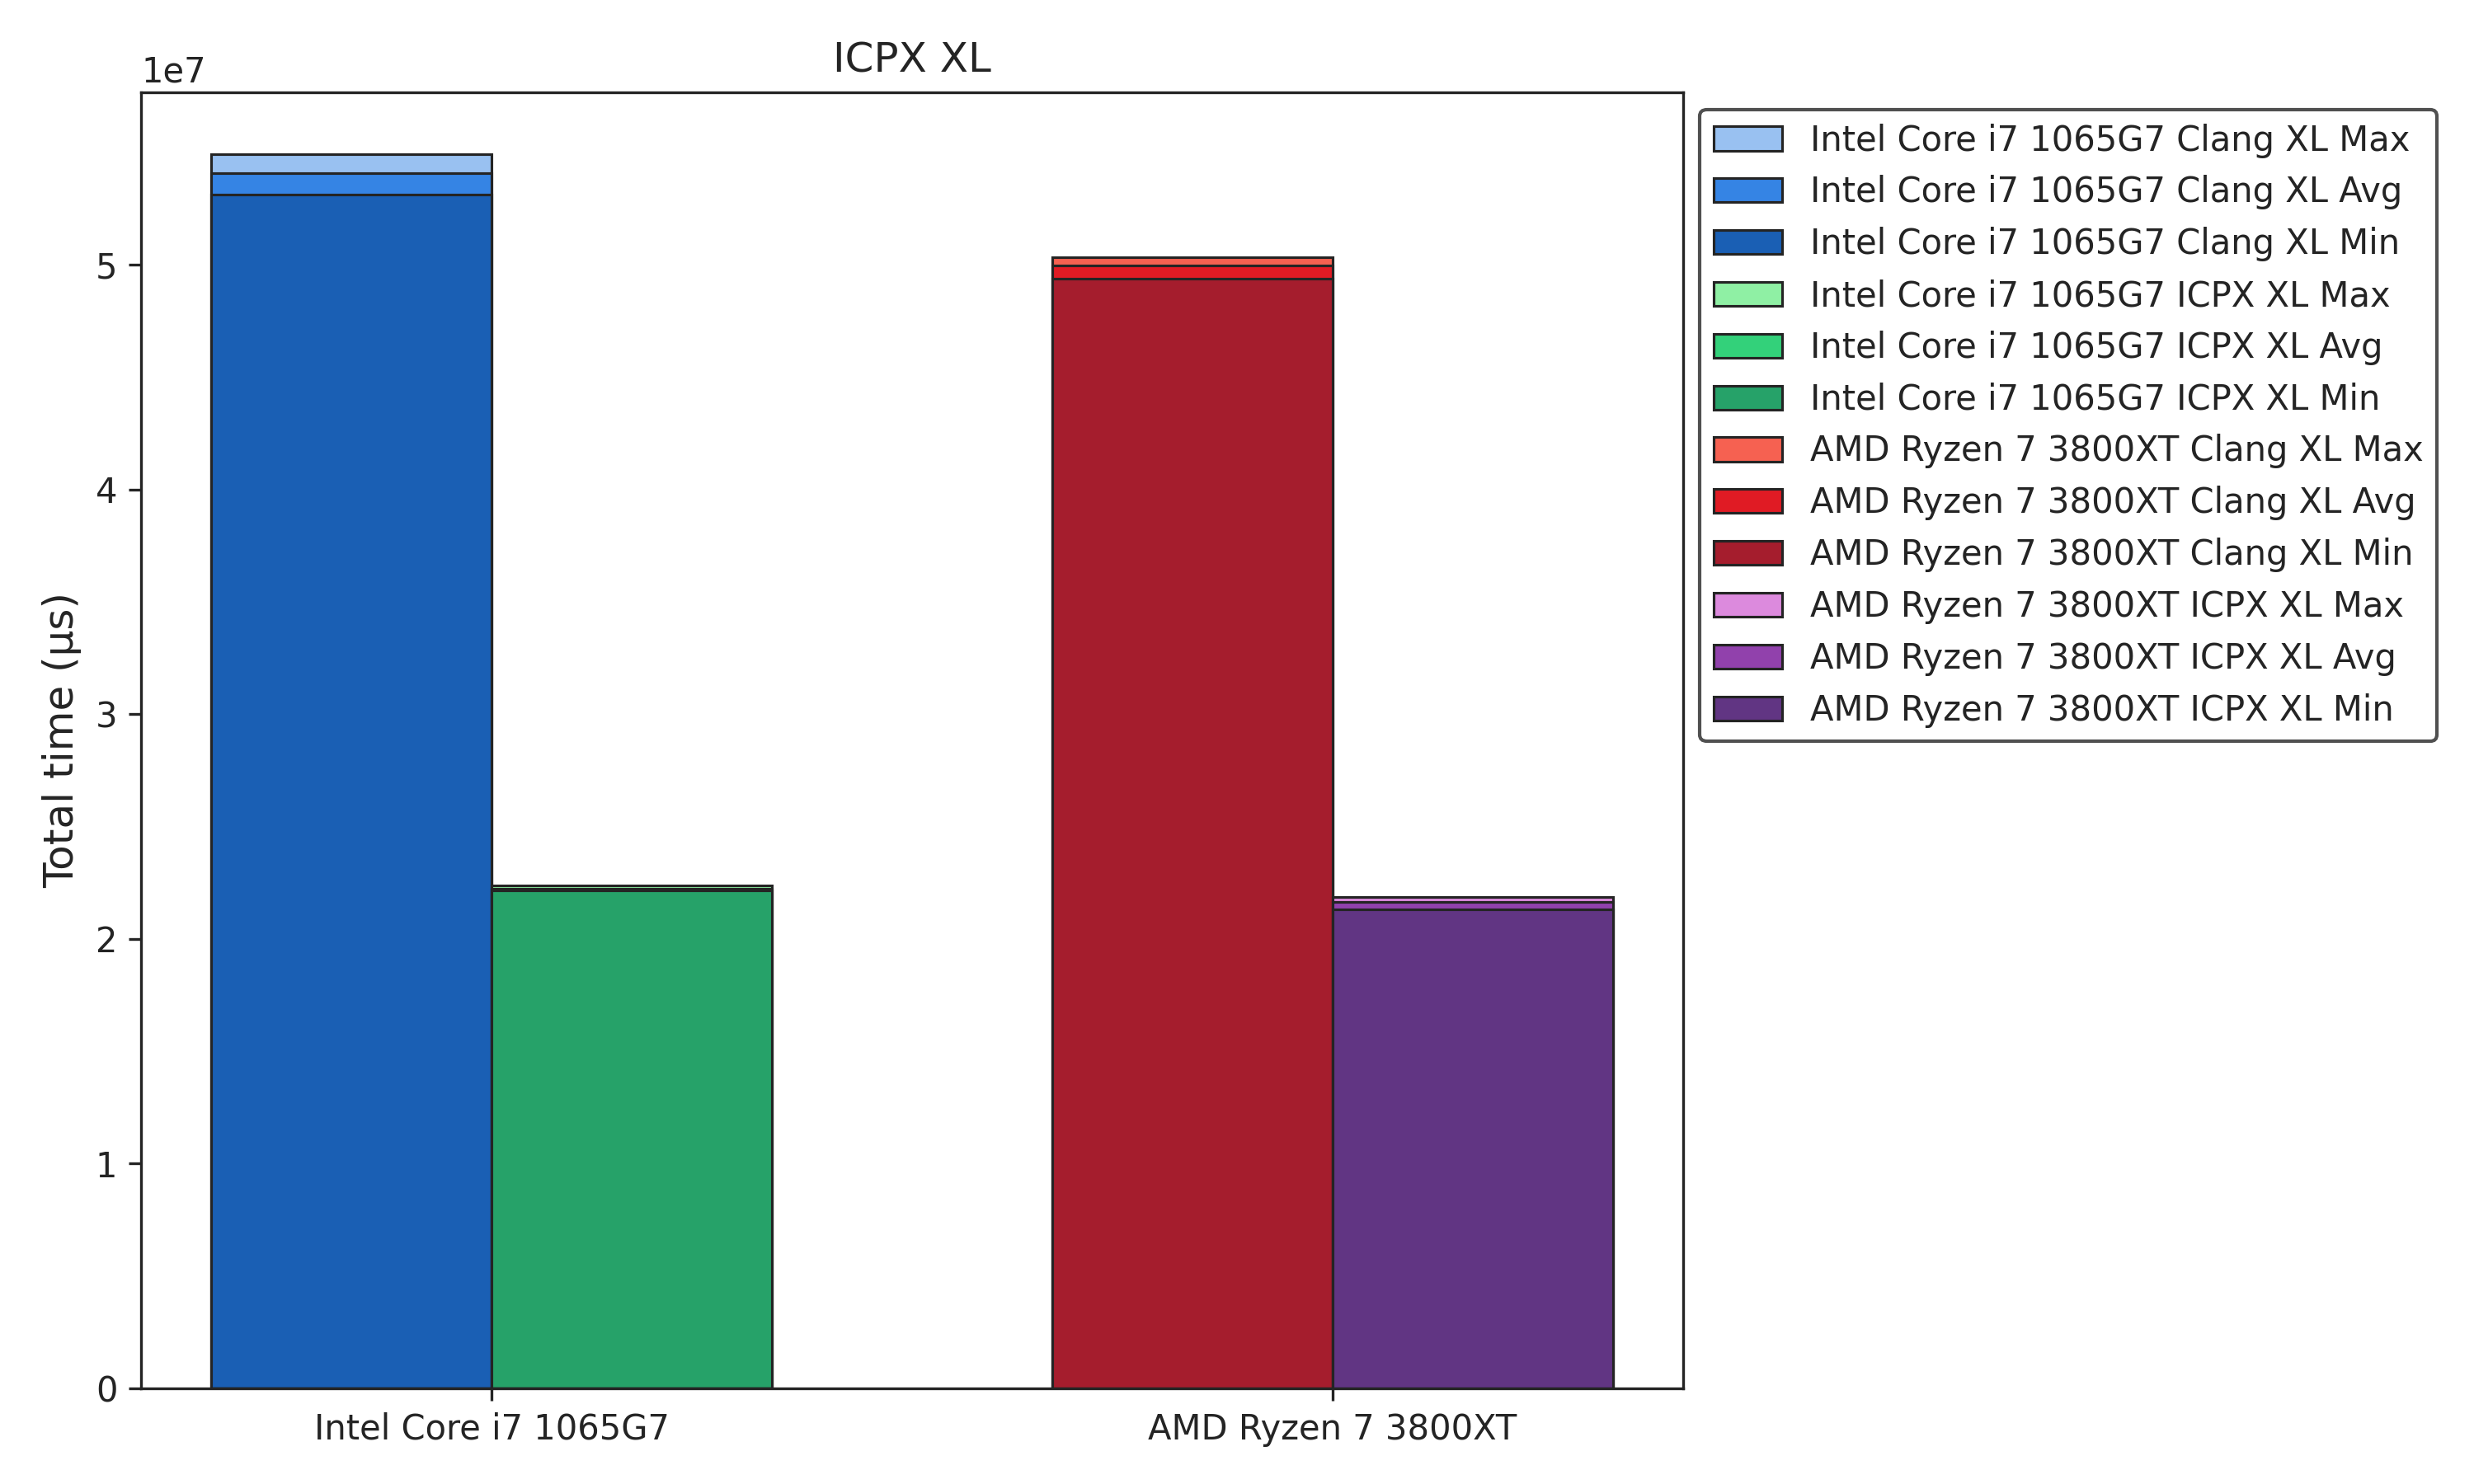
\includegraphics[width=\linewidth]{Graphs/ICPX XL.png}
  \caption{On the synthetic XL dataset}
 \label{fig:icpx_xl}
\end{subfigure}
\caption{Compiler performance benchmarks based on the naive implementation}
\label{fig:icpx}
\end{figure}
\begin{table}[htb!]
\centering
\caption{Compiler performance benchmarks based on the naive implementation\label{tab:icpx}}
\begin{tabular}{p{5cm} p{2cm} p{2cm} p{2cm} p{2cm}}
\hline
Benchmark Name & Minimum Value ($\mu$s) & Average Value ($\mu$s) & Maximum Value ($\mu$s) & Standard Deviation \\
\hline
Intel Core i7-1065G7 \\
\hspace{0.5cm}Clang & 41783.0 & 43833.5 & 47517.0 & 1788.0 \\
\hspace{0.5cm}ICPX & 16597.0 & 18605.9 & 22433.0 & 1833.4 \\
AMD Ryzen 7 3800XT \\
\hspace{0.5cm}Clang & 38841.0 & 39271.6 & 40180.0 & 379.2 \\
\hspace{0.5cm}ICPX & 14608.0 & 18121.6 & 32081.0 & 6855.0 \\
\hline
Intel Core i7-1065G7 \\
\hspace{0.5cm}Clang XL & 53137471.0 & 54097305.1 & 54939589.0 & 549782.2 \\
\hspace{0.5cm}ICPX XL & 22143313.0 & 22232581.5 & 22398563.0 & 71375.5 \\
AMD Ryzen 7 3800XT \\
\hspace{0.5cm}Clang XL & 49407386.0 & 49970509.5 & 50337761.0 & 318289.1 \\
\hspace{0.5cm}ICPX XL & 21312622.0 & 21658183.4 & 21861010.0 & 179367.3 \\
\hline
\end{tabular}
\end{table}
\FloatBarrier

The benchmark results based on the OpenMP implementation are shown in Figure~\ref{fig:icpx_openmp}, with the corresponding values listed in Table~\ref{tab:icpx_openmp}. The average performance of all CPUs on the MNIST dataset improves by 64.4\%. The average performance of the Intel Core i7-1065G7 improves by 64.2\% and the AMD Ryzen 7 3800XT improves by 64.5\%. The average performance of all CPUs on the synthetic XL dataset improves by 66.6\%. The Intel Core i7-1065G7 improves by 68.8\% and the AMD Ryzen 7 3800XT improves by 63.9\%.
\begin{figure}[htb!]
\centering
\begin{subfigure}{.5\textwidth}
  \centering
  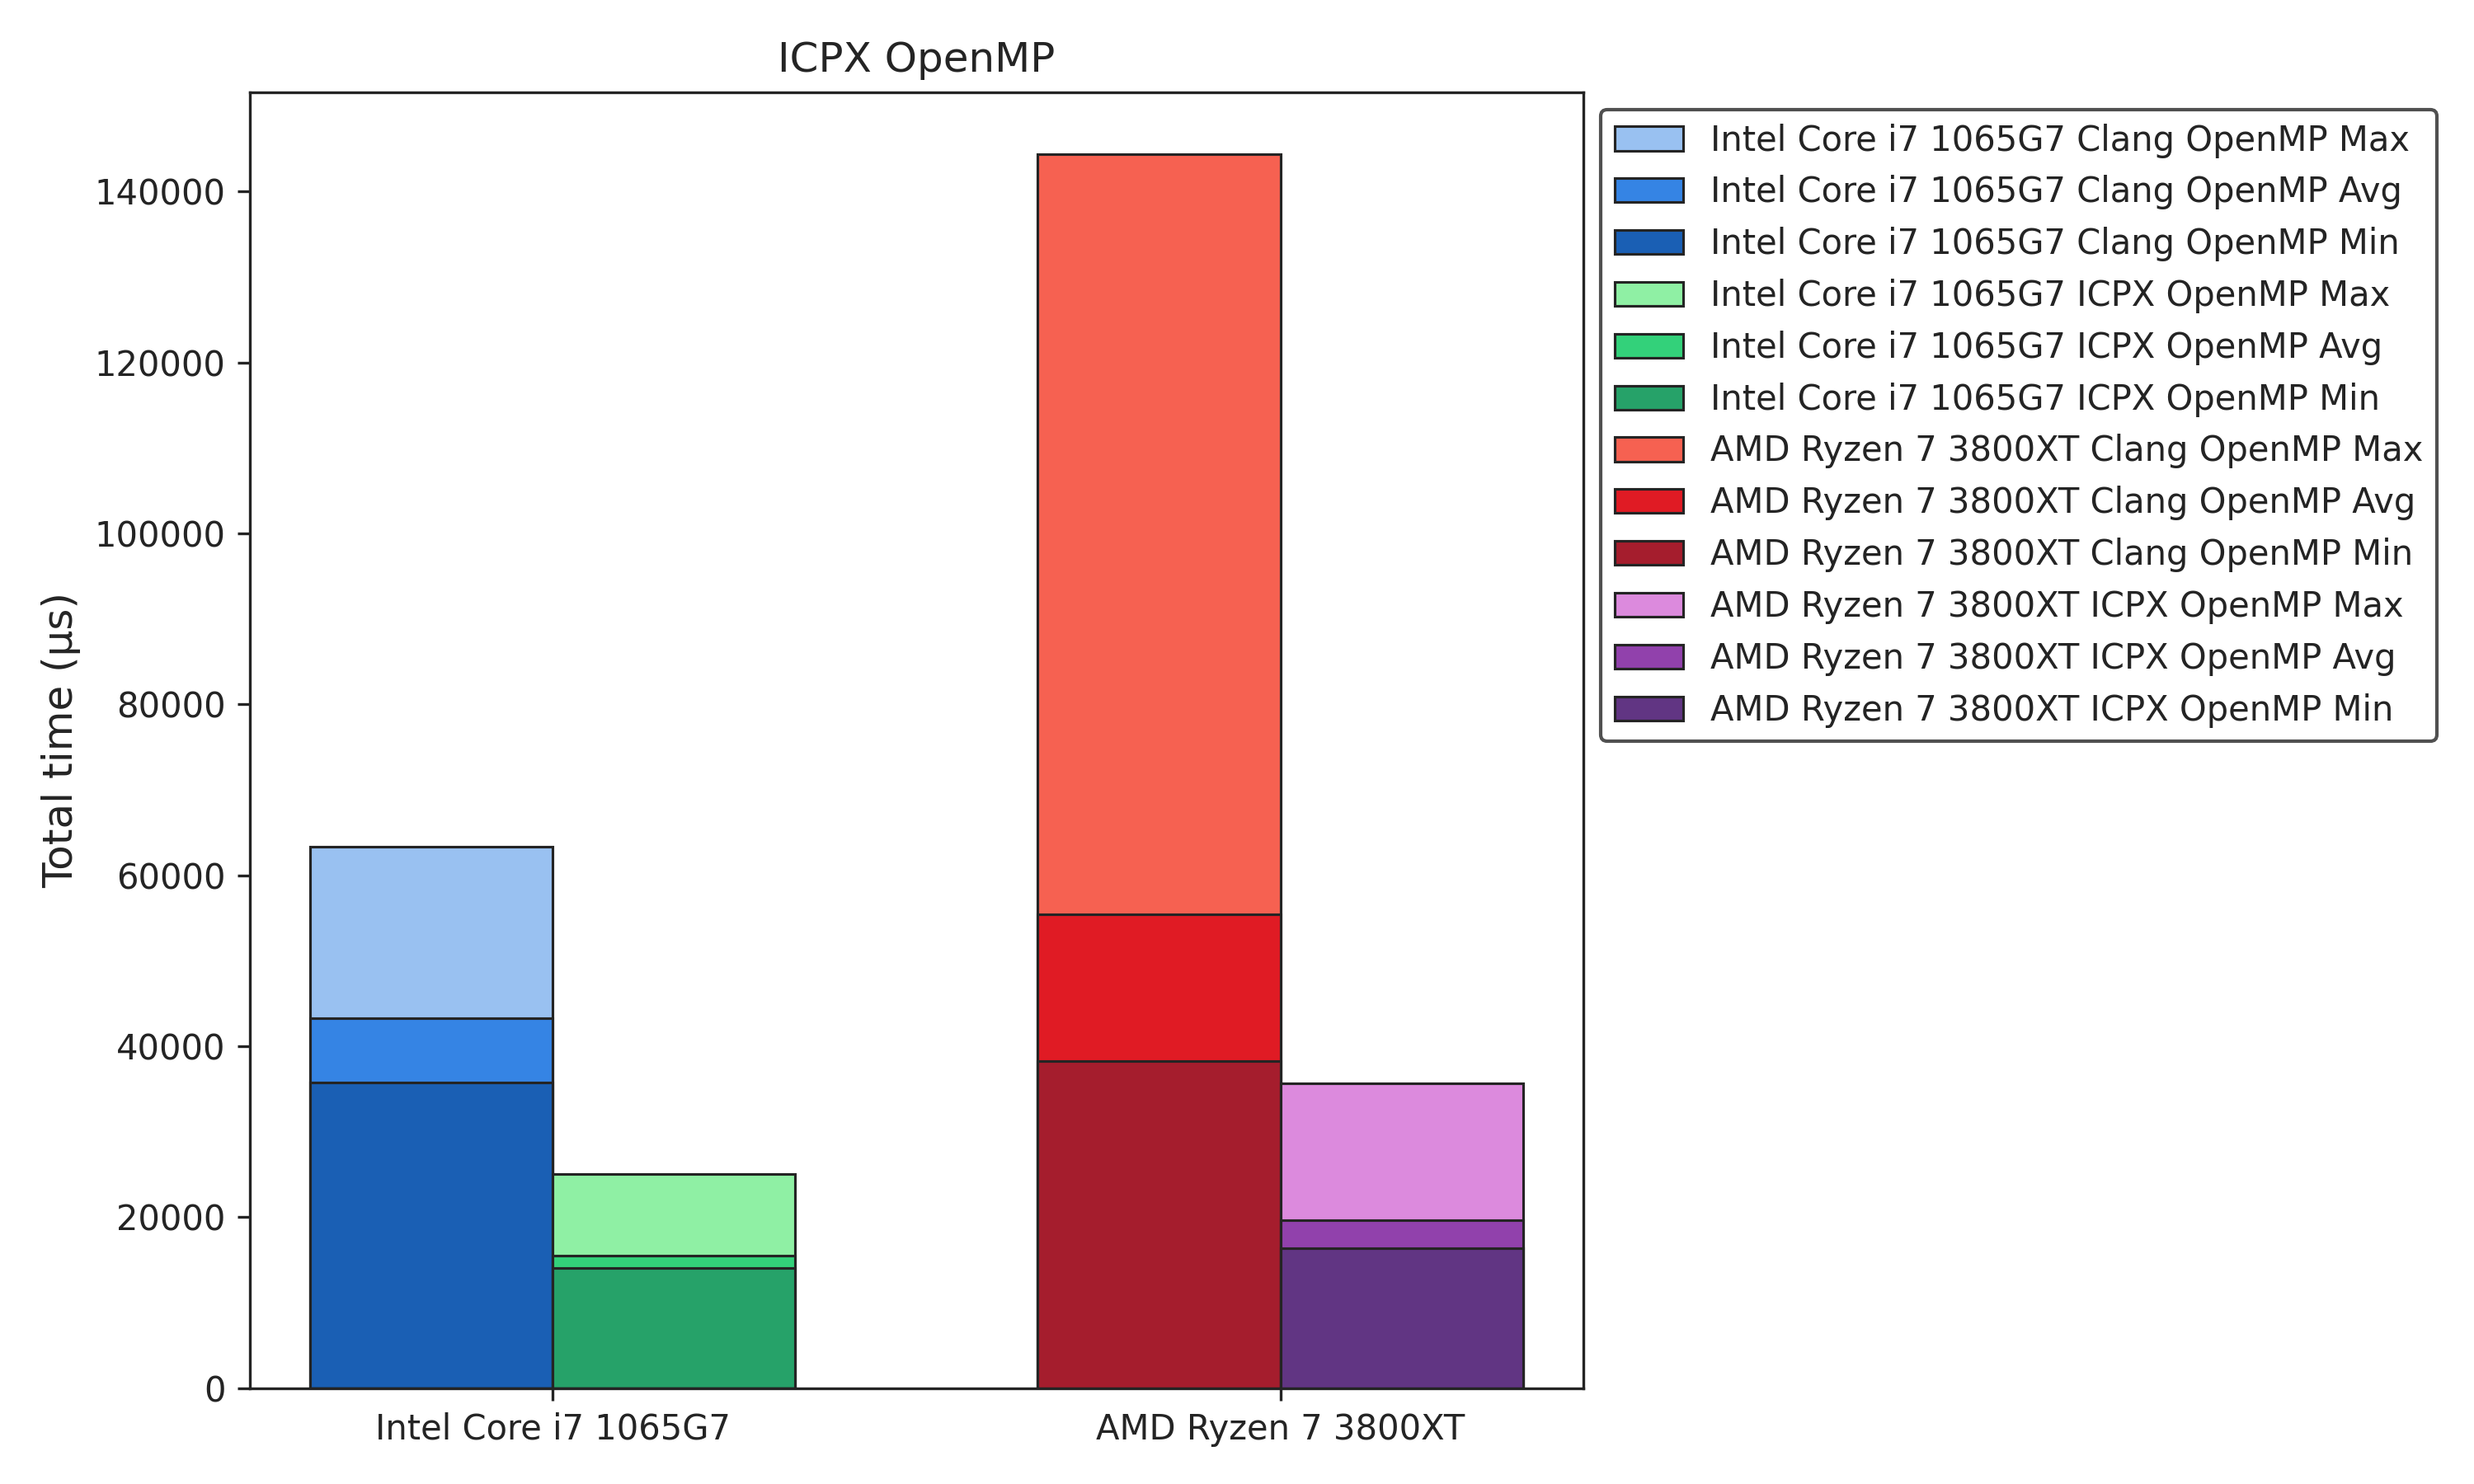
\includegraphics[width=\linewidth]{Graphs/ICPX OpenMP.png}
  \caption{On the MNIST dataset}
 \label{fig:icpx_openmp_mnist}
\end{subfigure}%
\begin{subfigure}{.5\textwidth}
  \centering
  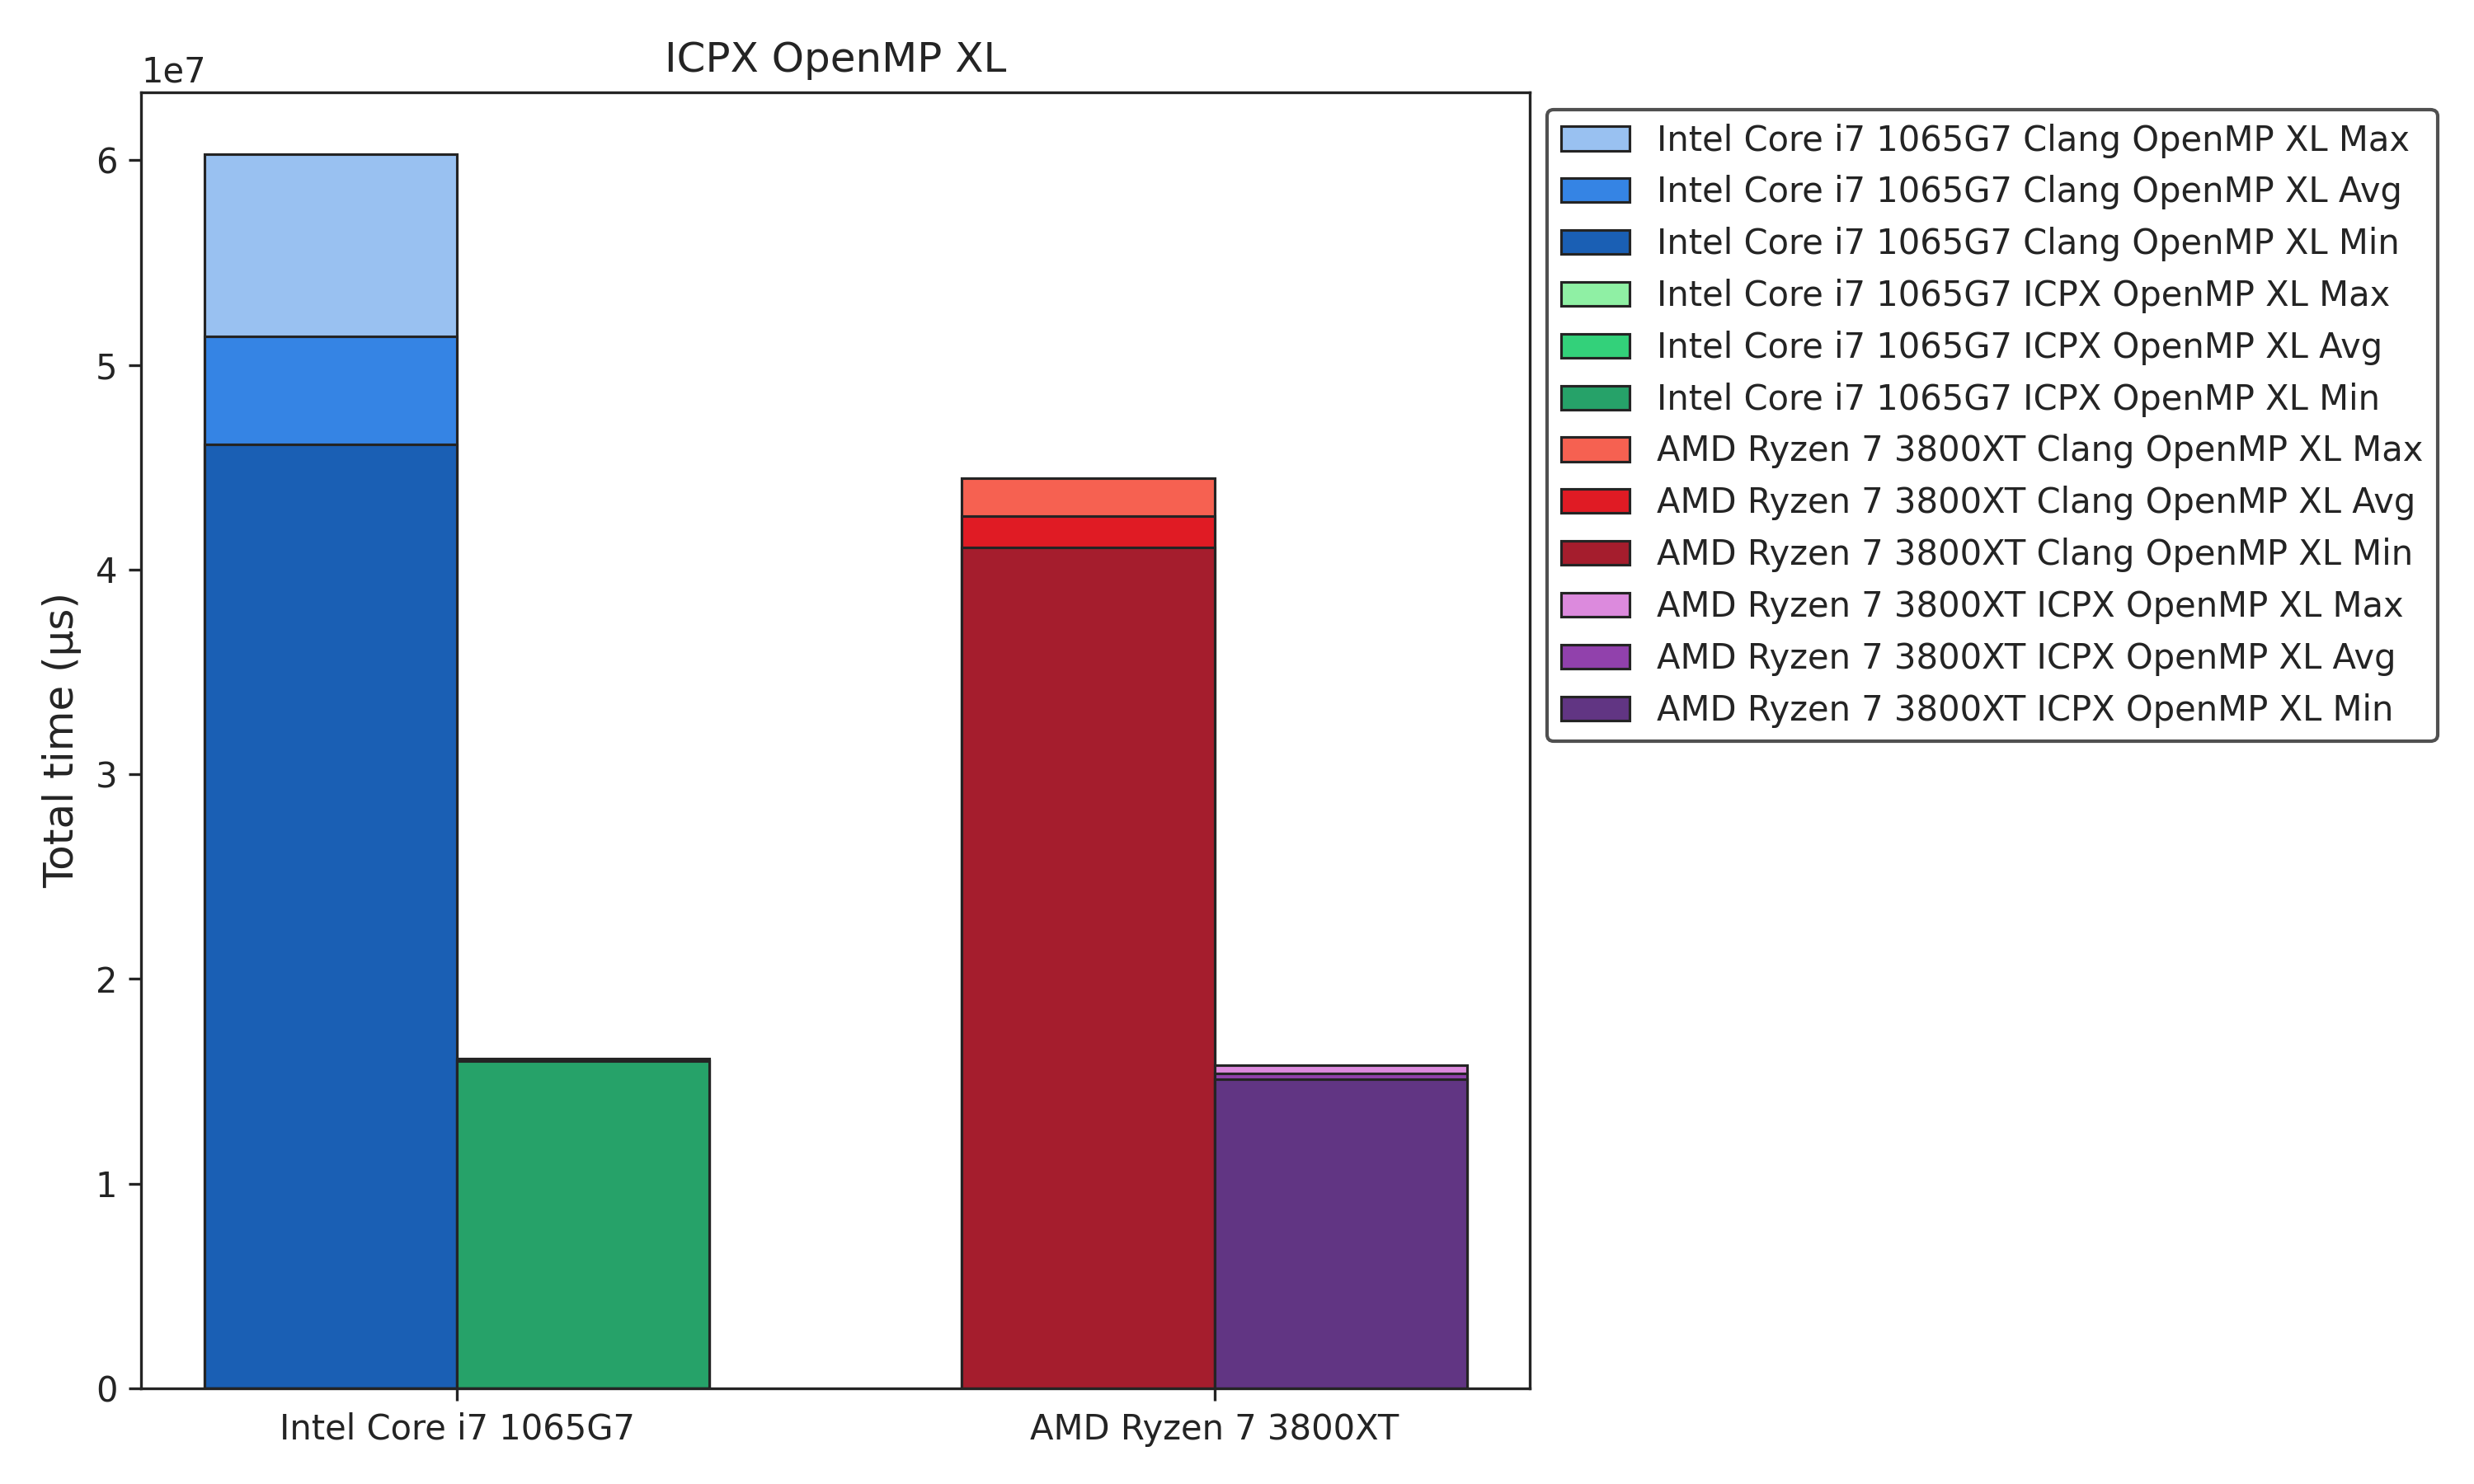
\includegraphics[width=\linewidth]{Graphs/ICPX OpenMP XL.png}
  \caption{On the synthetic XL dataset}
 \label{fig:icpx_openmp_xl}
\end{subfigure}
\caption{Compiler performance benchmarks based on the OpenMP implementation}
\label{fig:icpx_openmp}
\end{figure}
\begin{table}[htb!]
\centering
\caption{Compiler performance benchmarks based on the OpenMP implementation\label{tab:icpx_openmp}}
\begin{tabular}{p{5cm} p{2cm} p{2cm} p{2cm} p{2cm}}
\hline
Benchmark Name & Minimum Value ($\mu$s) & Average Value ($\mu$s) & Maximum Value ($\mu$s) & Standard Deviation \\
\hline
Intel Core i7-1065G7 \\
\hspace{0.5cm}Clang OpenMP & 35733.0 & 43297.5 & 63330.0 & 7658.0 \\
\hspace{0.5cm}ICPX OpenMP & 14062.0 & 15486.7 & 25067.0 & 3215.8 \\
AMD Ryzen 7 3800XT \\
\hspace{0.5cm}Clang OpenMP & 38261.0 & 55426.5 & 144388.0 & 31422.4 \\
\hspace{0.5cm}ICPX OpenMP & 16413.0 & 19668.4 & 35655.0 & 6414.5 \\
\hline
Intel Core i7-1065G7 \\
\hspace{0.5cm}Clang OpenMP XL & 46136509.0 & 51416232.8 & 60306735.0 & 4473869.3 \\
\hspace{0.5cm}ICPX OpenMP XL & 15978874.0 & 16047018.0 & 16112363.0 & 39602.5 \\
AMD Ryzen 7 3800XT \\
\hspace{0.5cm}Clang OpenMP XL & 41100356.0 & 42629449.5 & 44471702.0 & 1254546.1 \\
\hspace{0.5cm}ICPX OpenMP XL & 15098750.0 & 15372276.0 & 15783534.0 & 217075.1 \\
\hline
\end{tabular}
\end{table}
\FloatBarrier

The results are impressive and exceed expectations. It is evident that in three out of four cases, the Intel Compiler performs significantly better optimizations on Intel CPUs compared to AMD. However, both architectures benefit substantially, as anticipated. When using OpenMP, the performance gap between Clang and ICPX becomes even more pronounced. Interestingly, simply swapping the compiler driver can sometimes lead to optimizations as substantial as improving the code itself, without needing to modify anything. This demonstrates that the choice of compiler can have a significant impact on performance and should certainly be considered as a potential optimization strategy.
\subsubsection{Dialog}\label{subsec:dialog}
After significantly rewriting the Makefile for the Intel C++ Compiler, we now address an increasingly problematic issue: the uncontrolled growth in the number of Makefile targets. Each new optimization results in a new target, followed by another for the synthetic XL dataset, and additional ones for specific architectures or operating systems. As a result, the Makefile already contains 26 targets. This not only increases the length of the Makefile unnecessarily but also makes its maintenance nearly impossible.

Furthermore, the number of targets required in practice is even higher. For example, each optimization should ideally have a corresponding debug target. In total, there are over 1024 possible combinations of compiler flags (CFLAGS), each of which technically warrants its own Makefile target.

To resolve this issue, we decide to implement a Terminal User Interface (TUI). We expect this approach to not only reduce the development overhead but also significantly improve the user experience (UX) for future users of the framework. For this purpose, we choose the dialog utility, which enables the creation of interactive, text-based user interfaces within shell scripts. It offers a variety of widgets such as menus, checklists and forms, making it the perfect choice for our needs.\footnote{Dialog - An introductory tutorial: \url{https://dl.acm.org/doi/fullHtml/10.5555/324696.324702} (Jeff Tranter, 1994)}

As a first step, we design a flowchart diagram, shown in Figure~\ref{fig:goose}, to outline the interaction flow. We then implement the corresponding logic in a Bash script. Finally, we integrate the resulting script into our current source code Makefile as the config target, and into our global Makefile as the all target.
\begin{figure}[htb!]
    \centering
    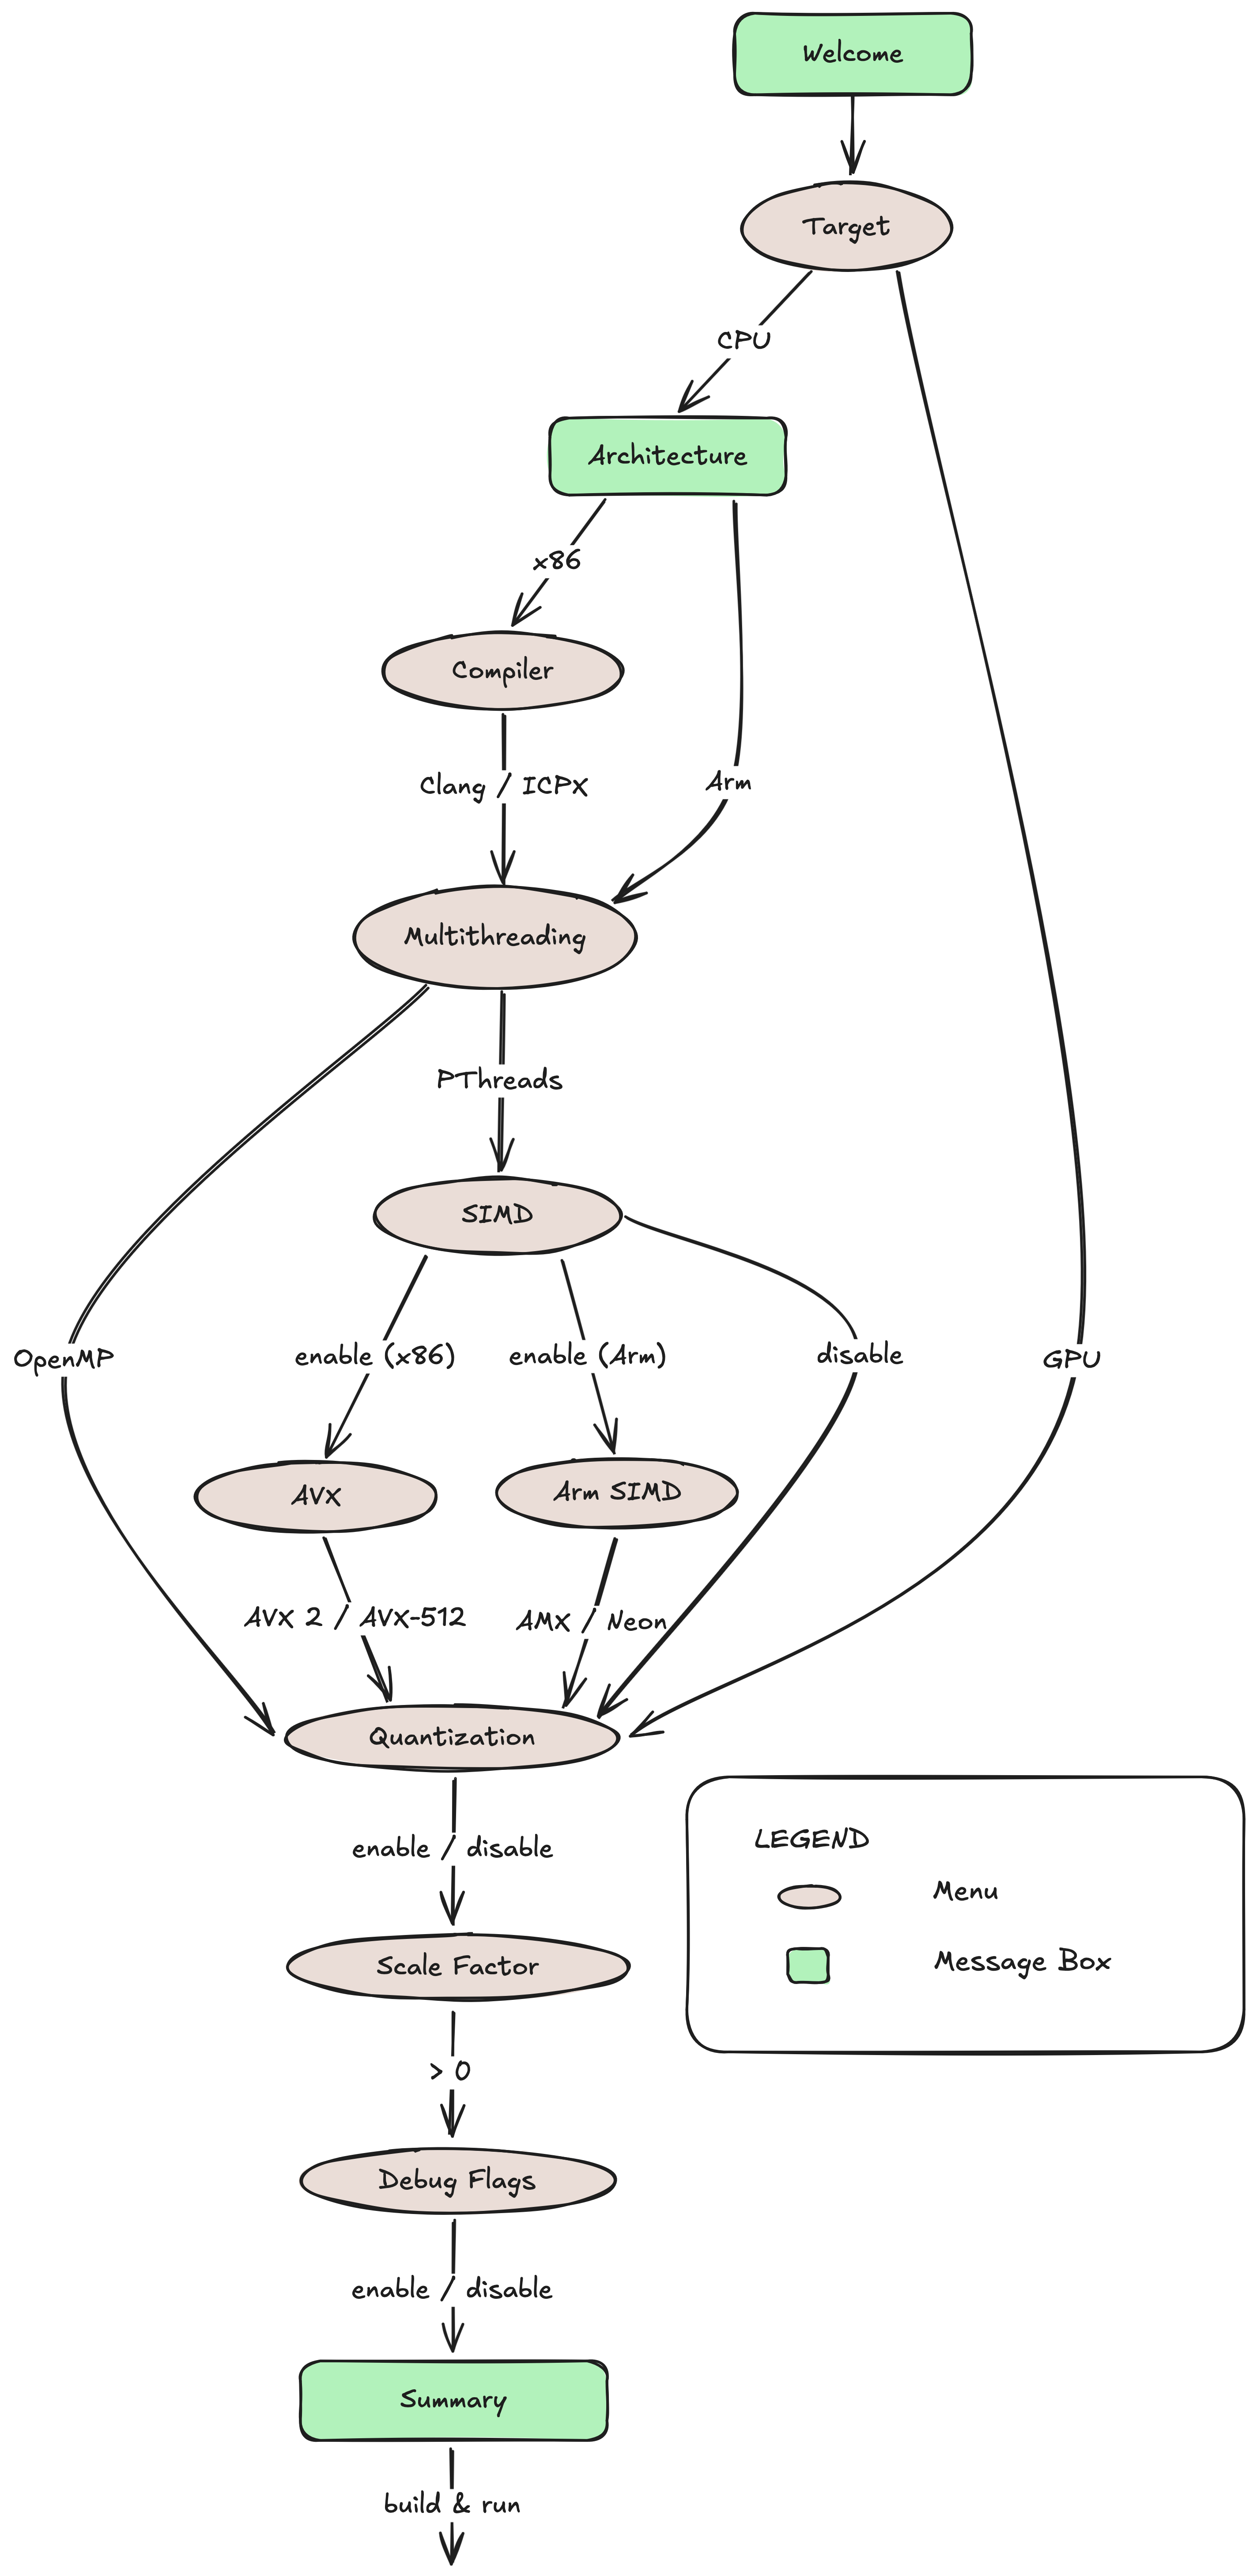
\includegraphics[width=0.4\linewidth]{Dialog/Goose.png}
    \caption{Flowchart illustrating the interaction flow implemented in the Bash script}
   \label{fig:goose}
\end{figure}

Listing~\ref{lst:dialog} demonstrates how we implement a simple menu to select between CPU and GPU execution. The resulting interface is illustrated in Figure~\ref{fig:dialog}.
\begin{lstlisting}[
    caption={Bash function implementing a simple dialog menu for target selection},
    label={lst:dialog},
    language=Bash,
    numbers=left,
    numbersep=10pt,
    basicstyle=\fontsize{10}{10}\selectfont,
    breaklines=true,
    postbreak=\mbox{\textcolor{red}{$\hookrightarrow$}\space},
    frame=single,
]
target() {
    TARGET=$(dialog --title "Target" --menu \
        "\nPlease select your desired target:" 10 60 2 \
        1 "CPU" \
        2 "GPU" \
        3>&1 1>&2 2>&3)
    if [[ $? -ne 0 ]]; then
        exit
    elif [[ "$TARGET" =~ "1" ]]; then
        uname
    elif [[ "$TARGET" =~ "2" ]]; then
        CC="nvcc"
        CFLAGS="$CFLAGS -DNVIDIA"
        architecture
        data_type
    fi
}
\end{lstlisting}
\begin{figure}[htb!]
    \centering
    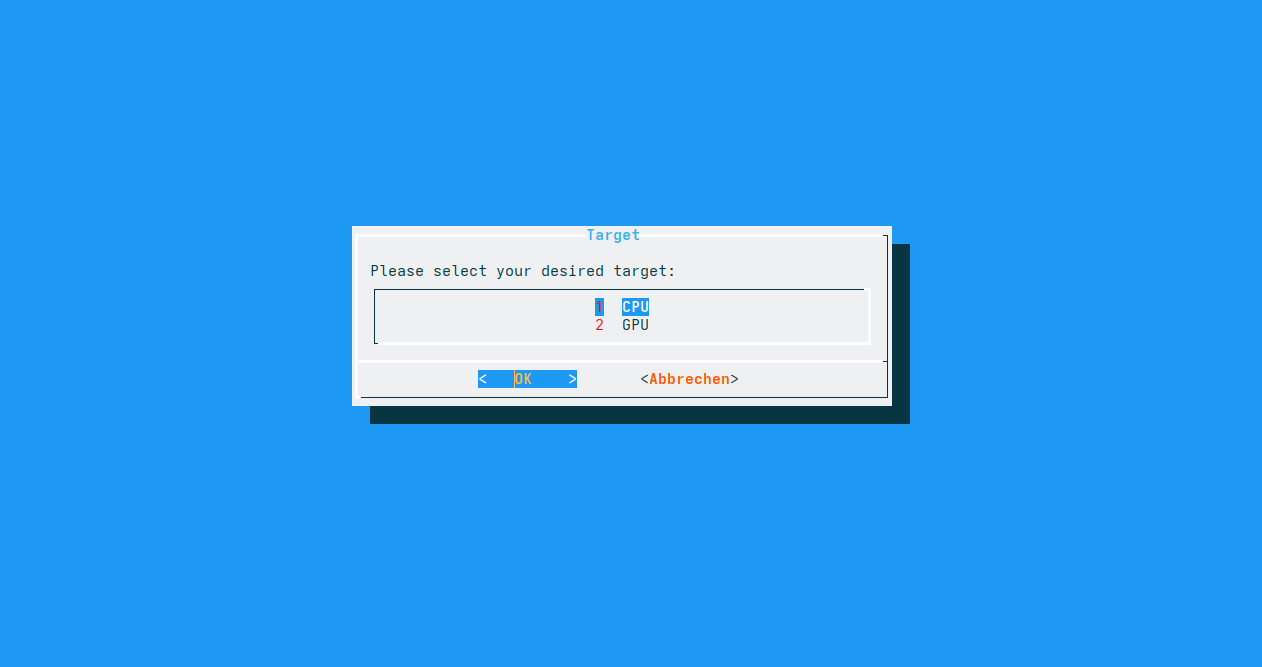
\includegraphics[width=\linewidth]{Dialog/Target.png}
    \caption{Dialog-based menu interface for selecting the target}
   \label{fig:dialog}
\end{figure}
\FloatBarrier
\subsection{SIMD}
\subsubsection{Overview of SIMD}\label{subsec:overview-of-simd}
In addition to the optimization methods previously discussed, we have also implemented Single Instruction, Multiple Data (SIMD) for the various architectures. SIMD enables the parallel execution of a single instruction on a set of data in one step, significantly reducing processing time. In general, SIMD utilizes vectors, in which the data is stored. The corresponding simultaneous operations are then performed on these vectors. This methodology is illustrated in Figure~\ref{fig:simd_architecture}.

\begin{figure}[htb!]
    \centering
    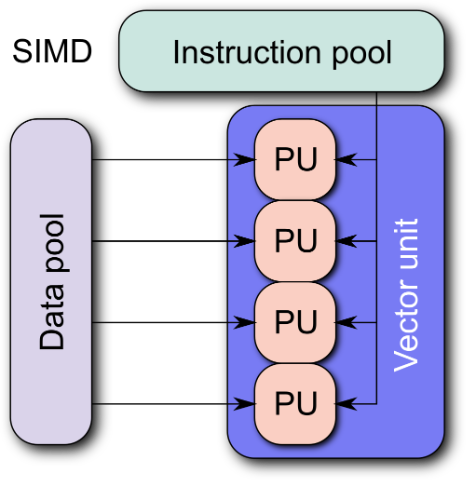
\includegraphics[width=0.4\linewidth]{SIMD/SIMD.png}
    \caption{SIMD Architecture\footnote{Single instruction, multiple data: \url{https://en.wikipedia.org/wiki/Single_instruction,_multiple_data} (accessed April 18, 2025; modified).}}
   \label{fig:simd_architecture}
\end{figure}

In this project, the framework was implemented using the following SIMD instructions:
\begin{itemize}
    \item AMD: SSE and AVX2 
    \item Arm: Neon, AMX 
    \item Intel: SSE, AVX2 and AVX-512
\end{itemize}

For the availability of the individual models on the respective architectures, we refer to the corresponding documentation.
\subsubsection{Arm Optimizations}\label{subsec:arm-optimizations}
\paragraph{Neon}
Arm Neon is an advanced SIMD (Single Instruction, Multiple Data) extension available in the Armv7 and Armv8 architectures. It is specifically designed to accelerate performance in applications that require intensive parallel data processing. By allowing multiple data elements to be processed simultaneously through a single instruction, Neon can offer substantial speed improvements over traditional scalar execution.\footnote{What is Neon?: \url{https://developer.arm.com/documentation/102467/0201/What-is-Neon-} (accessed April 18, 2025).}

Neon supports both integer and floating-point operations with vector widths of up to 128 bits. A typical Neon register file consists of 32 64-bit registers or alternatively 16 128-bit registers, which can be flexibly addressed. This enables the simultaneous processing of, for example, four 32-bit floats or 16 8-bit integer values, which becomes particularly relevant for quantization (see \ref{sec:quantization}) in our framework. Adapting the code to support quantization under Arm Neon is relatively straightforward. For a 32-bit floating-point load instruction, the following command is used: \texttt{vld1q\_f32}. Here, \texttt{vld1} stands for "vector load 1," which loads data from memory into a Neon register. The \texttt{q} stands for "quadword," indicating a 128-bit wide register, and \texttt{f32} refers to the data type. If a developer wishes to change the data type, for example to 8-bit integer values, the \texttt{f32} is replaced with \texttt{s8}. The rest of the instruction remains unchanged.

Additionally, the instruction \texttt{vaddvq\_f31} is worth highlighting, as it performs a horizontal addition on a vector. This means that all elements of the vector are summed, and the result is returned as a scalar value. This instruction is particularly useful for our implemented conv2d function.\footnote{Intrinsics: \url{https://developer.arm.com/architectures/instruction-sets/intrinsics/} (accessed April 18, 2025).}

Arm Neon also supports "unaligned data," meaning that as a programmer, one does not need to worry about alignment, which simplifies the implementation. Figure~\ref{fig:neon_loaddata} visually illustrates how data is loaded from memory into the registers.\footnote{Unaligned data access support: \url{https://developer.arm.com/documentation/ddi0388/b/unaligned-and-mixed-endian-data-access-support/unaligned-data-access-support} (accessed April 18, 2025).}

\begin{figure}[htb!]
    \centering
    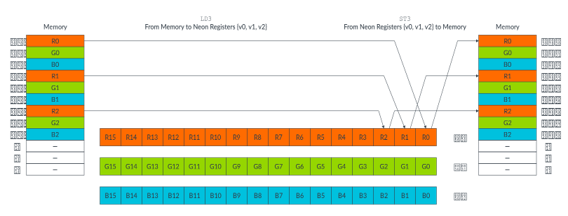
\includegraphics[width=\linewidth]{SIMD/Neon LoadData.png}
    \caption{Load Data from Memory to Register in Arm Neon\footnote{Load and store - data structures: \url{https://developer.arm.com/documentation/102159/0400/Load-and-store---data-structures} (accessed April 18, 2025).}}
   \label{fig:neon_loaddata}
\end{figure}

\paragraph{Performance Benchmarks}
The benchmark results are shown in Figure~\ref{fig:neon}, with the corresponding values listed in Table~\ref{tab:neon}. The average performance of the Apple M3 Pro 11-Core on the MNIST dataset improves by 5.2\%. The average performance of all CPUs on the synthetic XL dataset improves by 7.0\%.

\begin{figure}[htb!]
\centering
\begin{subfigure}{.5\textwidth}
  \centering
  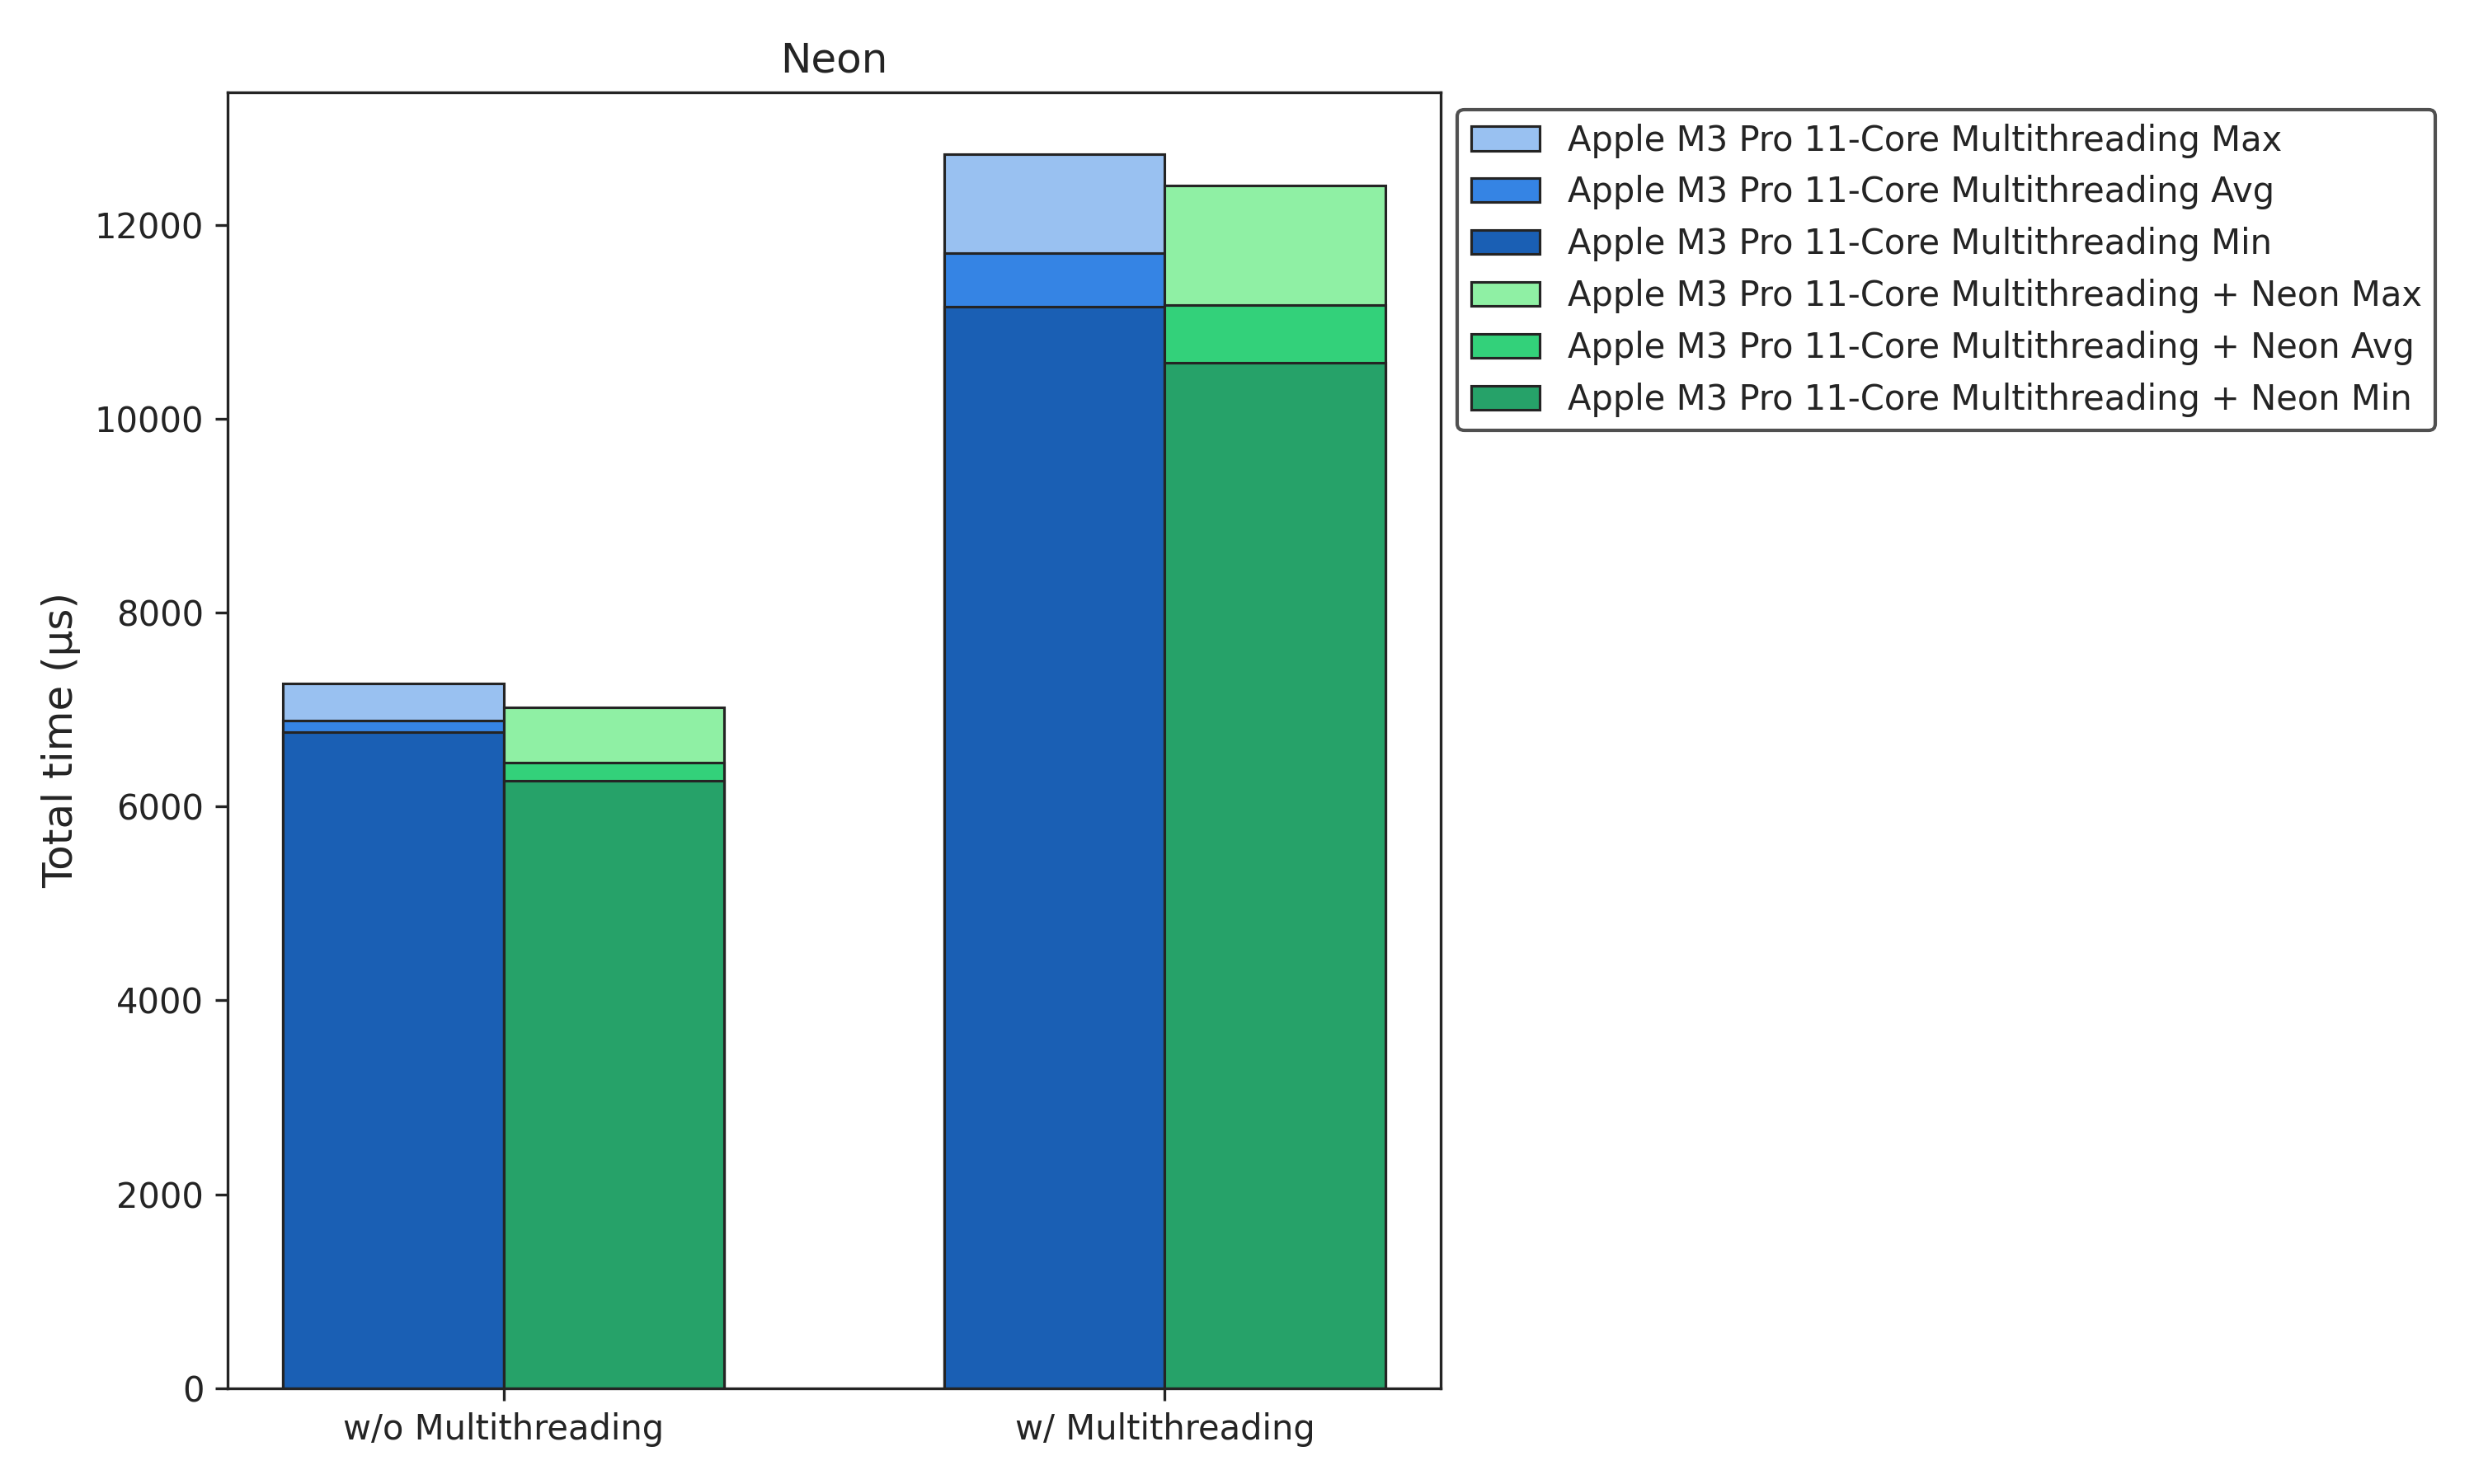
\includegraphics[width=\linewidth]{Graphs/Neon.png}
  \caption{On the MNIST dataset}
 \label{fig:neon_mnist}
\end{subfigure}%
\begin{subfigure}{.5\textwidth}
  \centering
  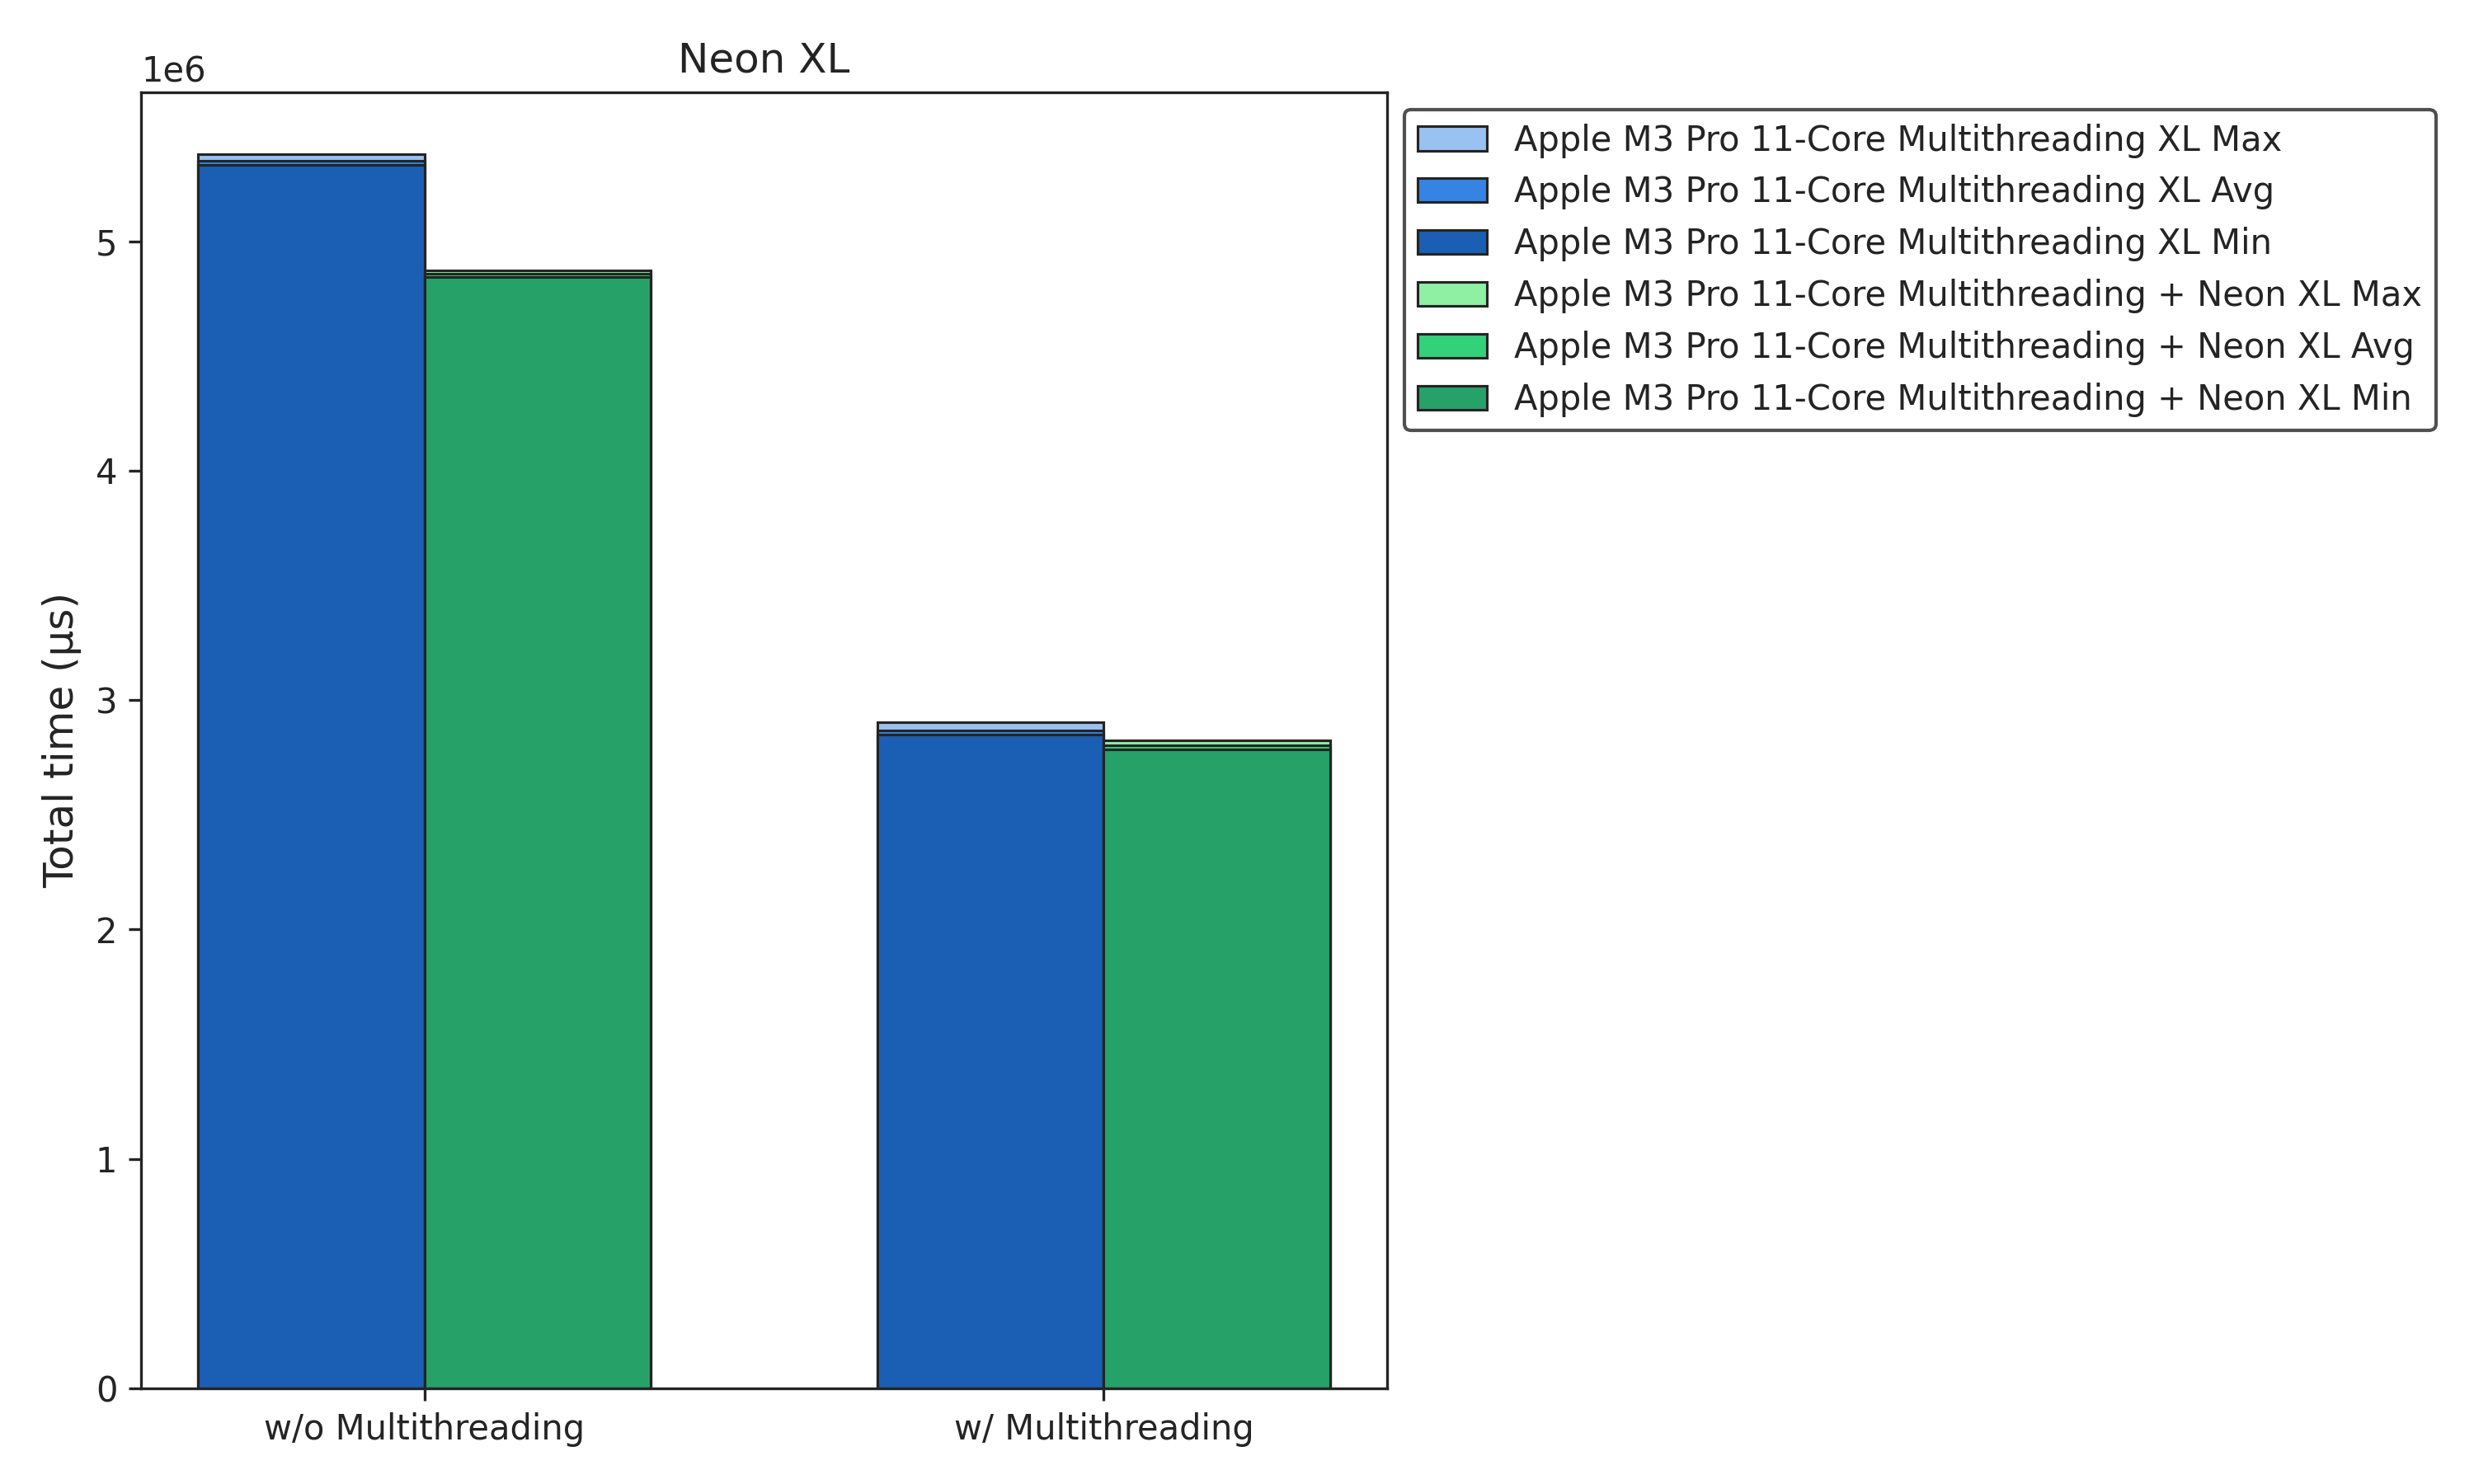
\includegraphics[width=\linewidth]{Graphs/Neon XL.png}
  \caption{On the synthetic XL dataset}
 \label{fig:neon_xl}
\end{subfigure}
\caption{Performance benchmarks of Arm Neon}
\label{fig:neon}
\end{figure}

\begin{table}[htb!]
\centering
\caption{Neon on Apple M3 Pro 11-Core\label{tab:neon}}
\begin{tabular}{p{5cm} p{2cm} p{2cm} p{2cm} p{2cm}}
\hline
Benchmark Name & Minimum Value ($\mu$s) & Average Value ($\mu$s) & Maximum Value ($\mu$s) & Standard Deviation \\
\hline
Multithreading & 11155.0 & 11707.3 & 12729.0 & 598.2 \\
Multithreading + Neon & 10575.0 & 11170.5 & 12407.0 & 618.4 \\
\hline
Multithreading XL & 2848506.0 & 2867258.2 & 2903430.0 & 19278.1 \\
Multithreading + Neon XL & 2783871.0 & 2802165.9 & 2824752.0 & 13541.5 \\
\hline
\end{tabular}
\end{table}
\FloatBarrier

The implementation of Arm Neon and SIMD resulted in performance improvements in both the MNIST and synthetic XL benchmarks. These improvements can be attributed to the application of the multithreading approach combined with the processing of 128 bits per instruction. Consequently, these results align with expectations. 
It is worth noting that Arm Neon on the current M4 Apple Silicon chips has transitioned to Armv9 with Scalable Matrix Extensions (SME), which is expected to contribute to a seven percent performance boost. This extension supports 256-bit vector lengths.\footnote{Apple ist beim M4 zu ARMv9 gewechselt: \url{https://www.golem.de/news/cpu-entwicklung-apple-ist-beim-m4-zu-armv9-gewechselt-2405-185431.html} (accessed April 18, 2025).}

\paragraph{AMX}
In addition to Arm Neon vector operations, Apple provides further optimization capabilities, most notably through the Neural Engine (NPU), the GPU, and the AMX (Apple Matrix Extension) chip. However, the NPU and GPU were not utilized in this project, as their integration into our C++ framework would not have been seamless.
For instance, integrating the NPU would have required converting our network into a CoreML model, followed by various (post-)quantization steps for optimization. Utilizing the GPU, on the other hand, would have necessitated the use of Xcode and the Metal compiler — tools that are not natively available on all Apple Silicon devices and involve additional setup and installation effort.
As a result, we focused on integrating the AMX (Apple Matrix Extension) chip, available in Apple’s Arm-based silicon lineup (M1, M2, etc.).

AMX instructions are officially undocumented; therefore, we relied on a GitHub repository that has reverse-engineered the AMX instruction set. To verify whether AMX instructions are supported, we recommend executing the provided Makefile, which triggers a series of tests. The result of this test is shown in Listing~\ref{lst:amx_test}.

\begin{lstlisting}[
    caption={AMX Compatibility Test},
    label={lst:amx_test},
    language=Bash,
    numbers=left,
    numbersep=10pt,
    basicstyle=\fontsize{10}{10}\selectfont,
    breaklines=true,
    postbreak=\mbox{\textcolor{red}{$\hookrightarrow$}\space},
    frame=single,
]
gcc -O2 -g test.c ldst.c extr.c fma.c fms.c 
genlut.c mac16.c matfp.c matint.c vecfp.c 
vecint.c ./a.out

Testing AMX_LDX... OK
Testing AMX_LDY... OK
# [...]
Testing AMX_STZ... OK
# [...]
Testing AMX_FMA32... OK
# [...]
\end{lstlisting}

As shown in Listing~\ref{lst:amx_test}, all instructions are supported. Before presenting the implementation in detail, we briefly provide an overview of AMX. There are four X and four Y registers, which serve as source registers for computations. In total, these can store up to 64 floating-point values. The Z register acts as the target register or accumulator and is capable of holding a 64×64 floating-point matrix.

In the header file \texttt{aarch64.h}, the necessary assembly instructions are defined as macros. Bitmasks (hereafter referred to as "bm") are used to control the behavior of individual instructions. The following key instructions can be found in the code:

\begin{itemize}
    \item \texttt{AMX\_SET()} and \texttt{AMX\_CLR()} to mark relevant AMX regions within the code,
    \item \texttt{AMX\_LDX(bm)} and \texttt{AMX\_LDY(bm)} to load values in the source register,
    \item \texttt{AMX\_STZ(bm)} to store values in the target register and
    \item \texttt{AMX\_FMA32(bm)} to perform a fused-multiply-addition.
\end{itemize}

The aforementioned instructions were implemented for the non-quantized model, as AMX does not support the 8-bit integer data type, which is used as input for our quantized model.

Since the AMX instruction set does not support simple addition but only fused multiply-add operations—which combine both multiplication and addition, as in \texttt{FMA(x,y,z): z[\_][i] += x[i] * y[i]} — AMX is only used in the functions \texttt{matmul\_simd()} and \texttt{conv2d\_simd()}.

For a detailed description of the bitmasks and the individual functions, we refer to the documentation available in the GitHub repository.\footnote{Instructions: \url{https://github.com/corsix/amx/blob/main/Instructions.md} (accessed April 18, 2025).}

\paragraph{Power Consumption}
In addition to the benchmarks presented in the following section, we also measured the power consumption. For this purpose, we used the tool "powermetrics" and manually calculated the average power consumption during runtime. The measured values are listed in Table~\ref{tab:amx_power}.

\begin{table}[htb!]
\centering
\caption{AMX vs. Neon - Power Consumption during Runtime\label{tab:amx_power}}
\begin{tabular}{p{3cm} p{5cm}}
\hline
Benchmark Name & Power Consumption (mW) \\
\hline
AMX MNIST & 7.331 \\ 
Neon MNIST & 7.331 \\ 
\hline
AMX XL & 7.218 \\
Neon XL & 7.340 \\
\hline
\end{tabular}
\end{table}
\FloatBarrier

It is immediately apparent that for small problem sizes (see MNIST), there is no significant difference in power consumption between Neon and AMX. However, for larger problems, the AMX chip appears to be approximately 1.7\% more energy-efficient. This can be attributed to the full utilization of the systolic array, which is only achieved with larger problem sets.

\paragraph{Performance Benchmarks}
The benchmark results are shown in Figure~\ref{fig:amx}, with the corresponding values listed in Table~\ref{tab:amx}. The average performance of the Apple M3 Pro 11-Core on the MNIST dataset decreases by 7.4\%. The average performance of Apple M3 Pro 11-Core on the synthetic XL dataset improves by 1.0\%.

\begin{figure}[htb!]
\centering
\begin{subfigure}{.5\textwidth}
  \centering
  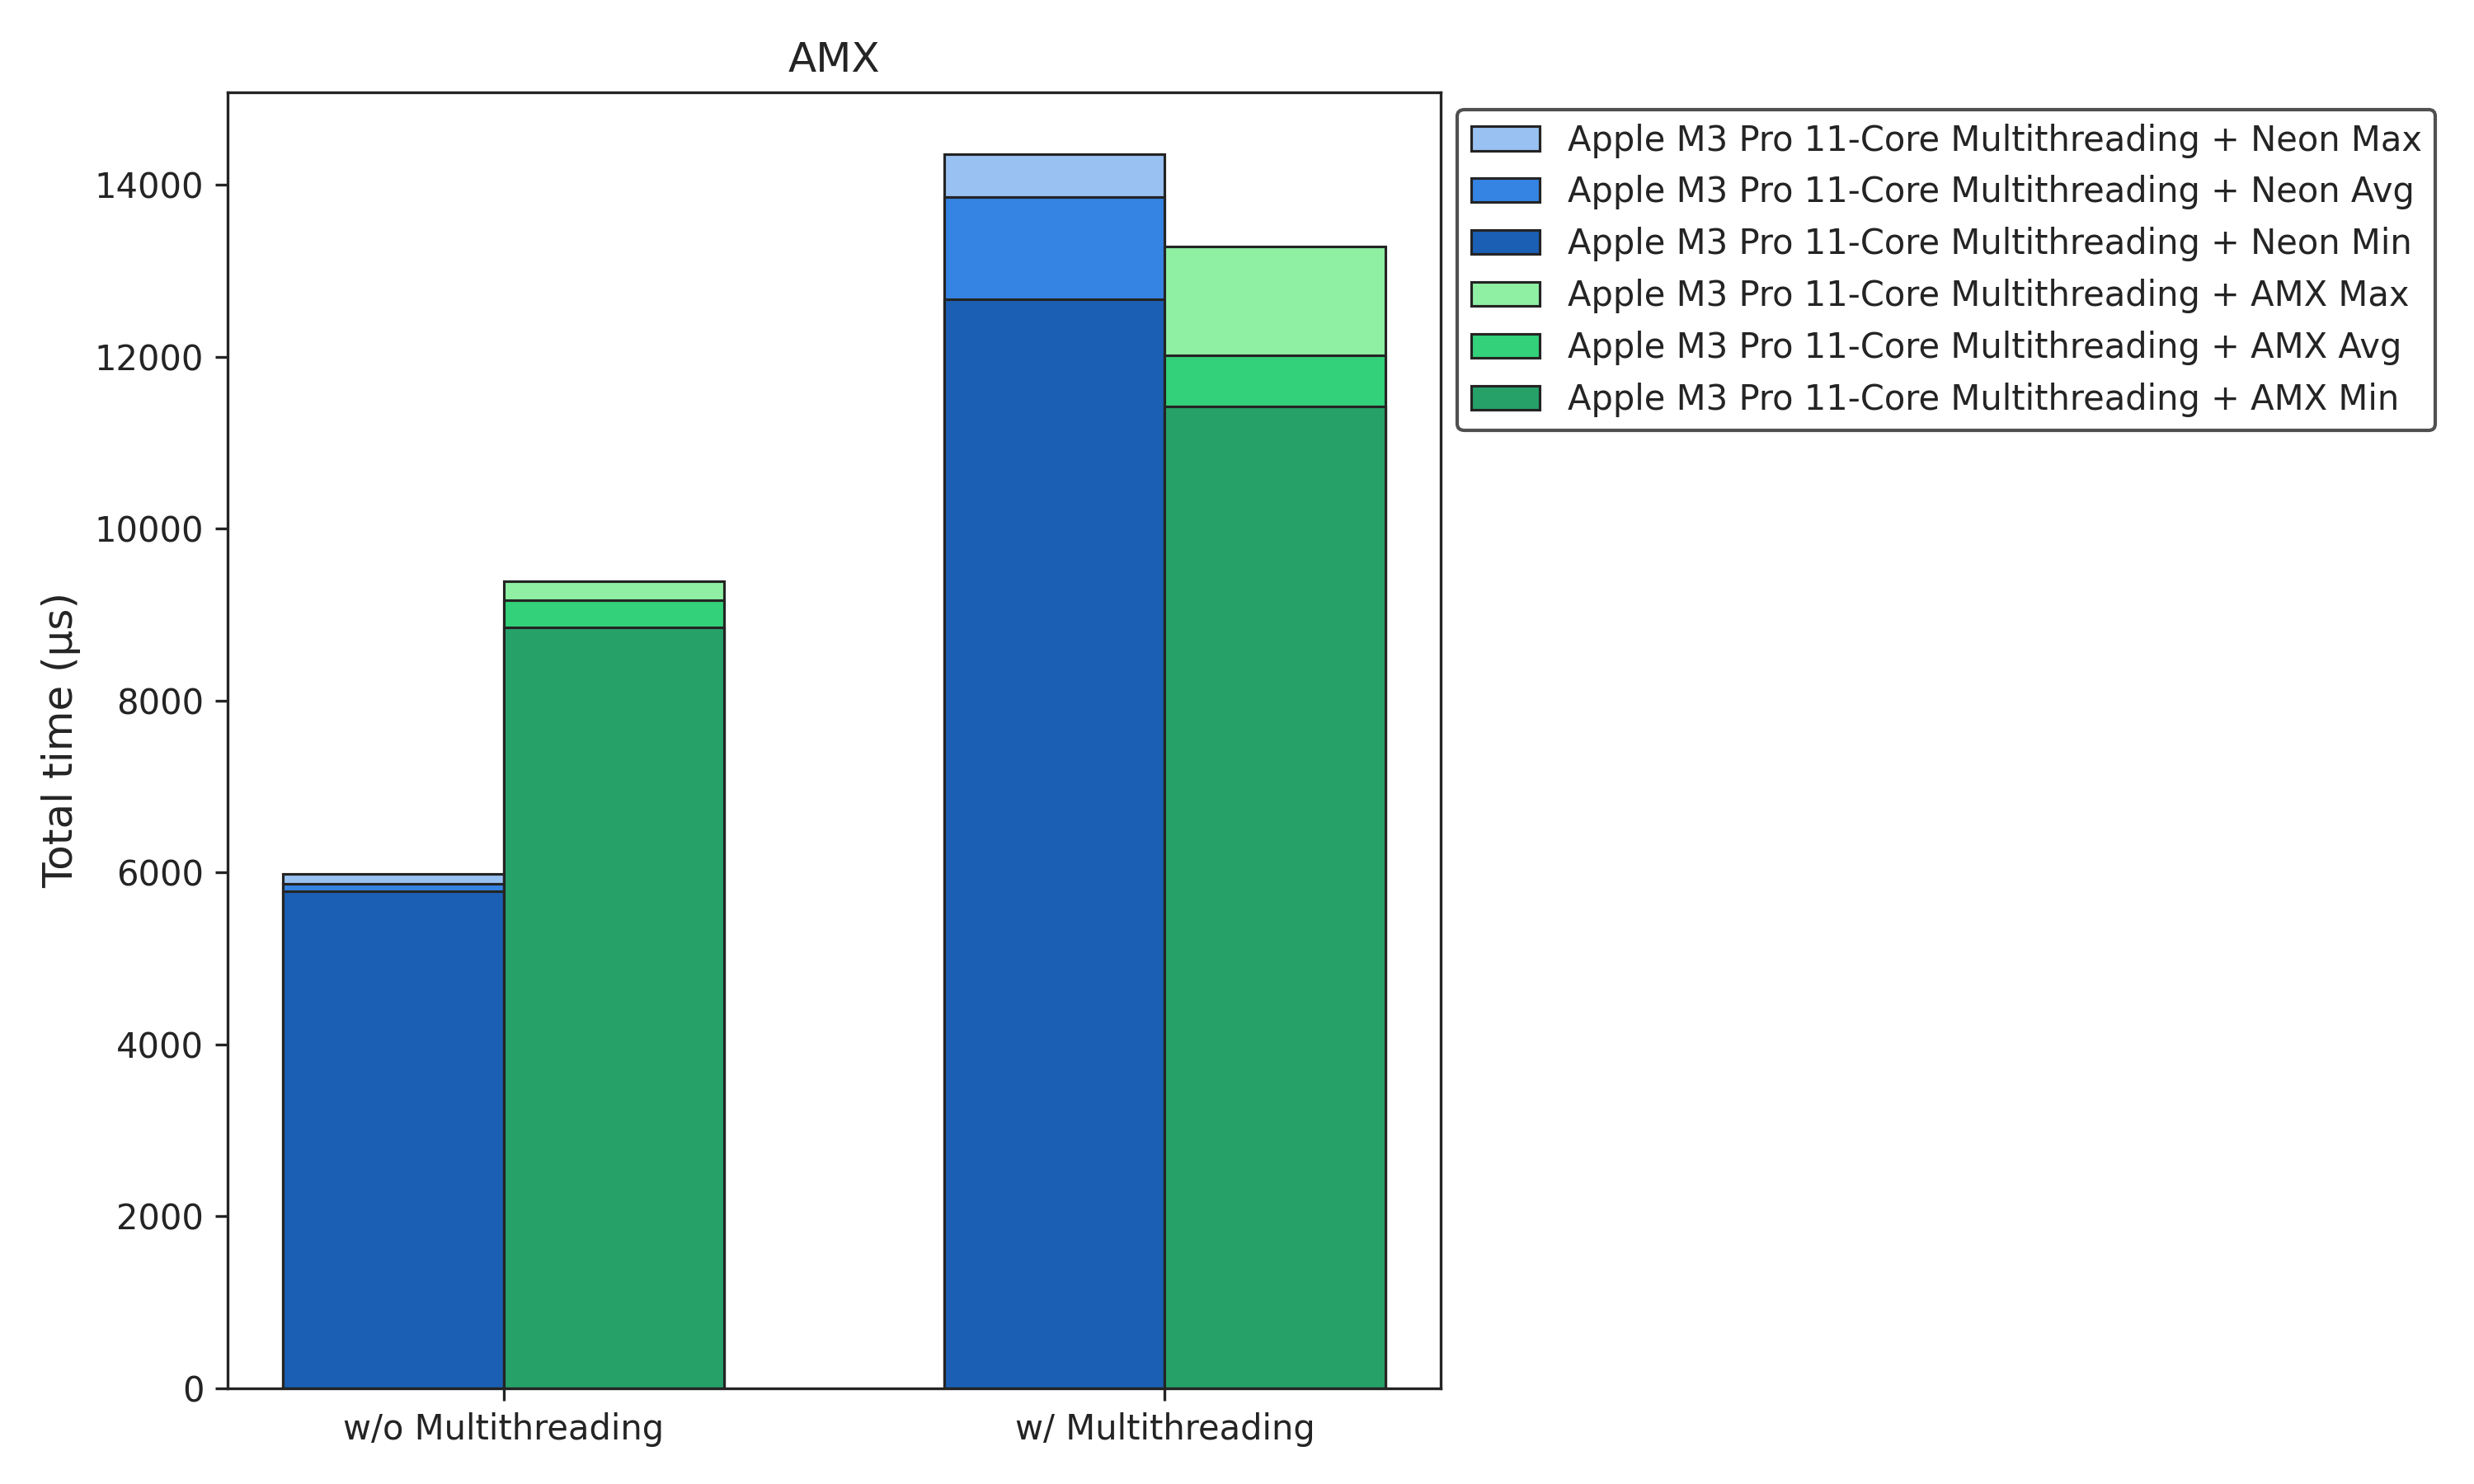
\includegraphics[width=\linewidth]{Graphs/AMX.png}
  \caption{On the MNIST dataset}
 \label{fig:amx_mnist}
\end{subfigure}%
\begin{subfigure}{.5\textwidth}
  \centering
  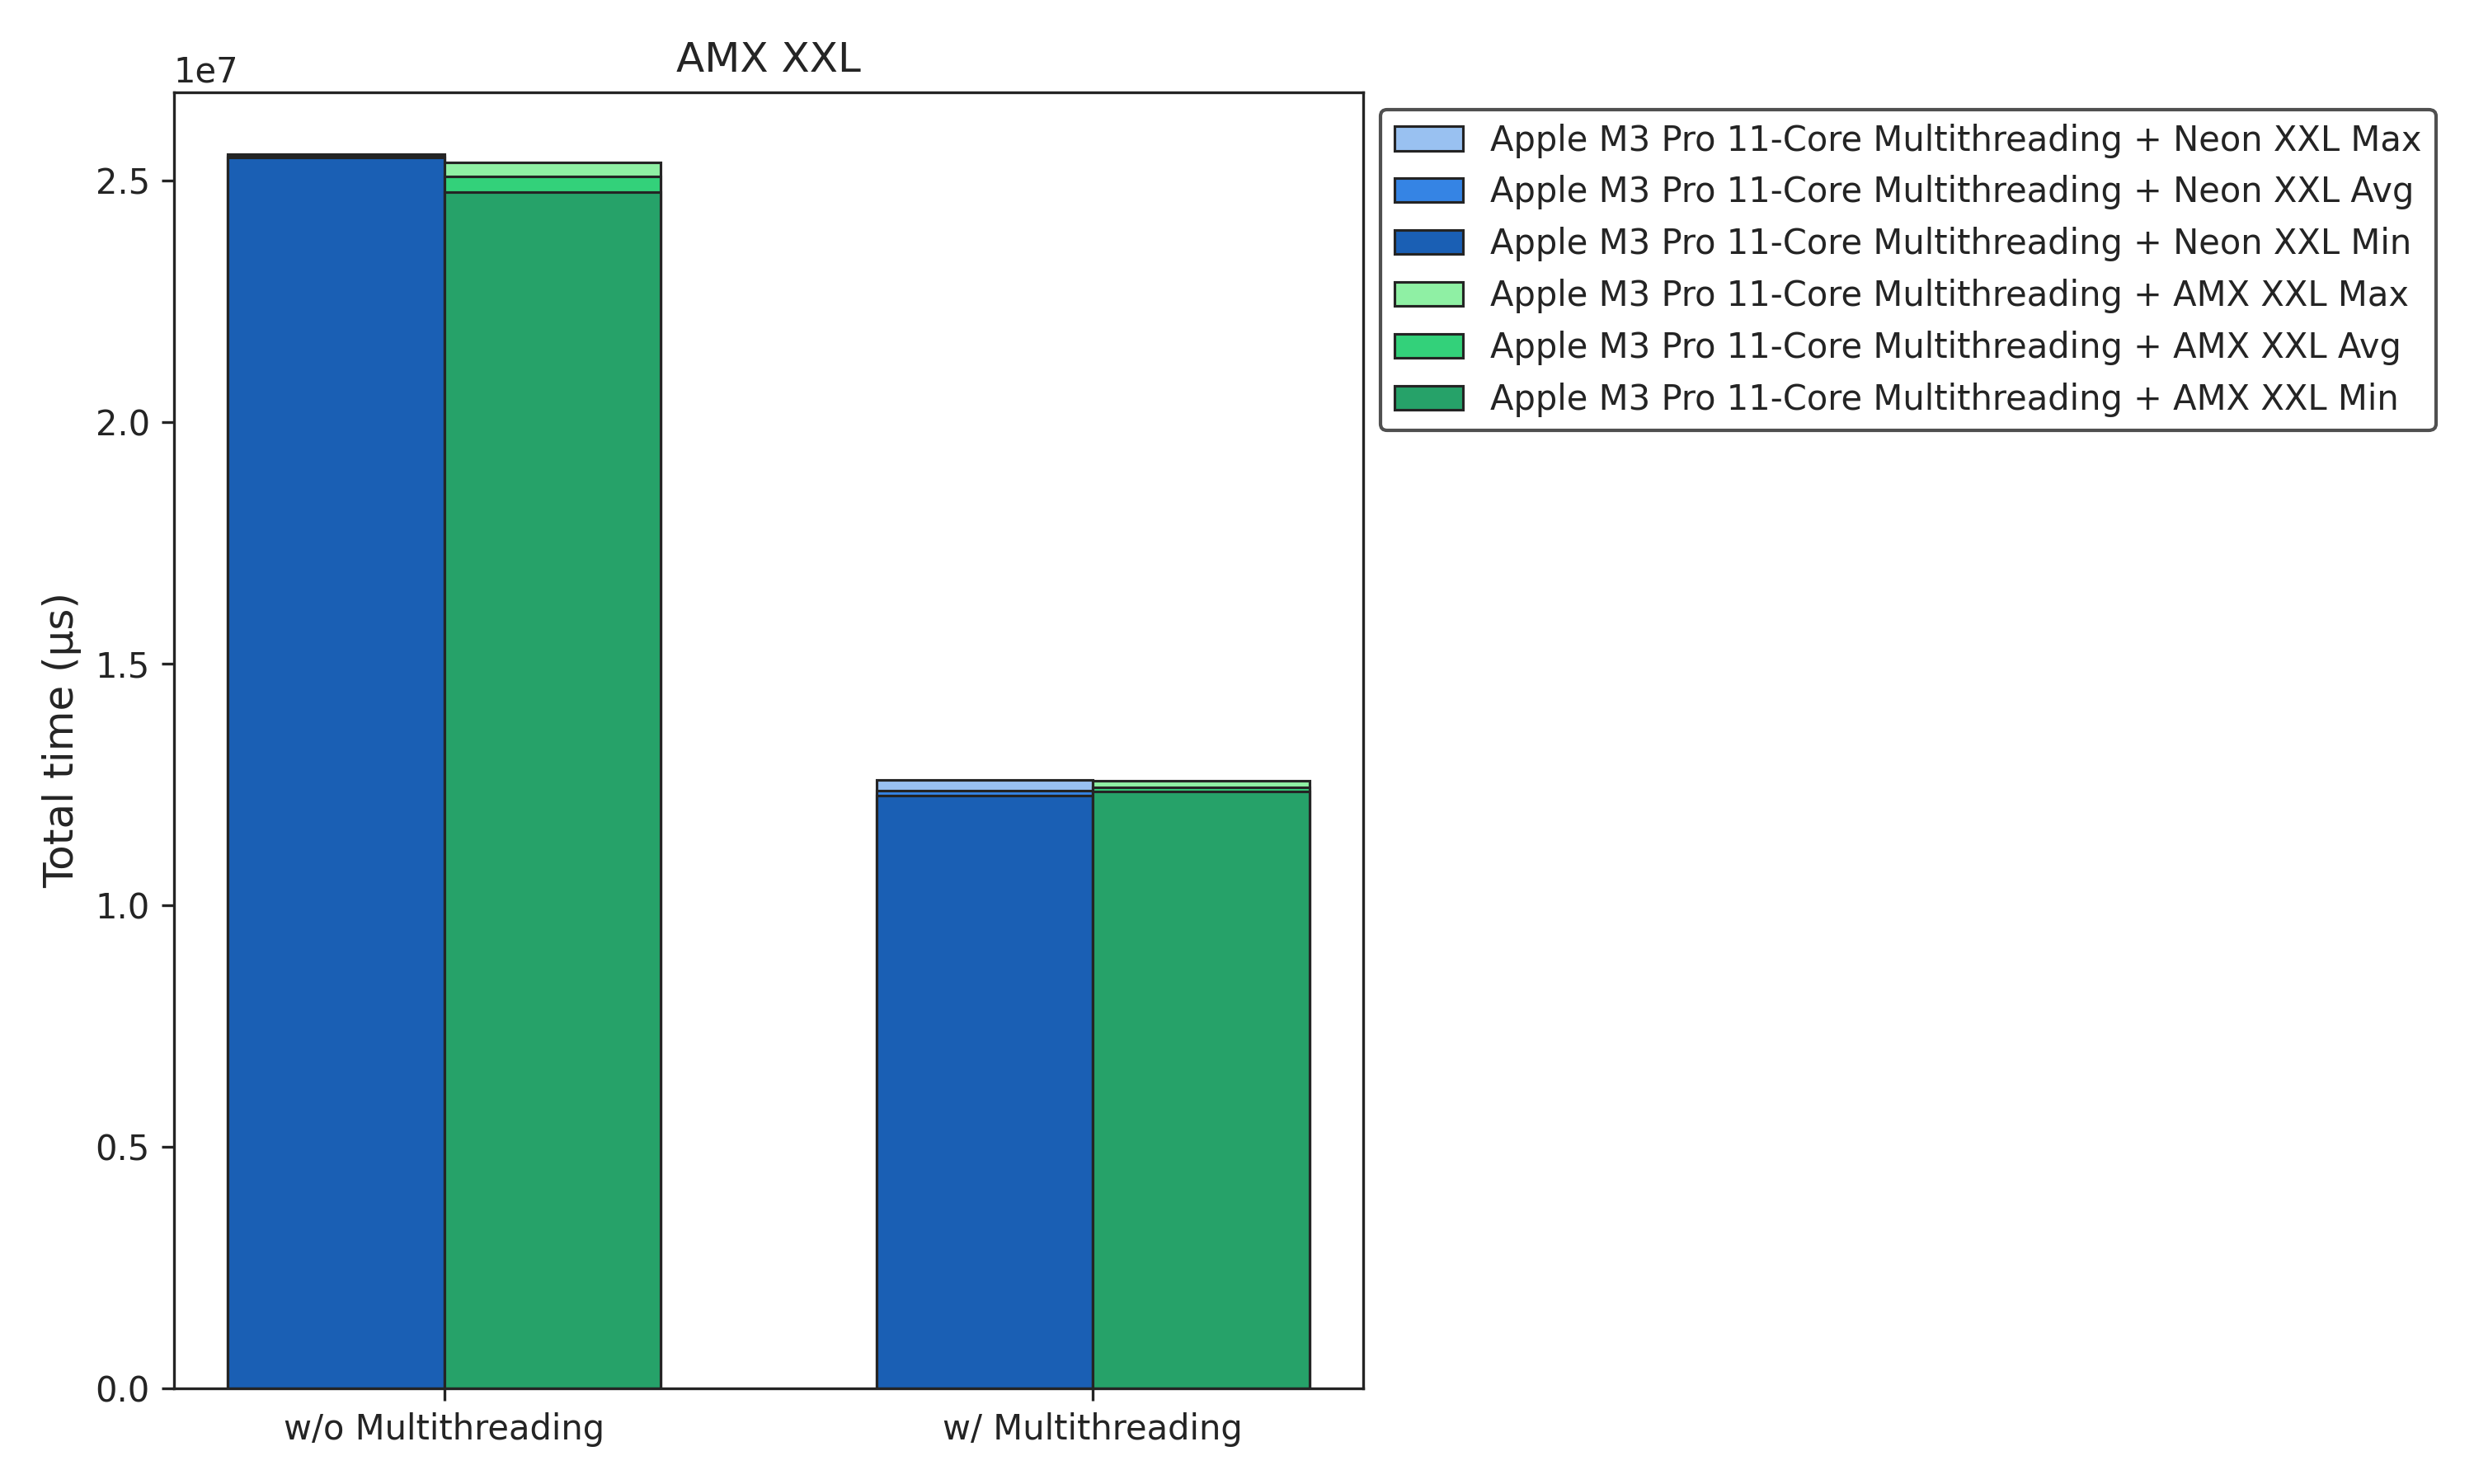
\includegraphics[width=\linewidth]{Graphs/AMX XXL.png}
  \caption{On the synthetic XXL dataset}
 \label{fig:amx_xxl}
\end{subfigure}
\caption{Performance benchmarks of AMX}
\label{fig:amx}
\end{figure}

\begin{table}[htb!]
\centering
\caption{AMX on Apple M3 Pro 11-Core\label{tab:amx}}
\begin{tabular}{p{5cm} p{2cm} p{2cm} p{2cm} p{2cm}}
\hline
Benchmark Name & Minimum Value ($\mu$s) & Average Value ($\mu$s) & Maximum Value ($\mu$s) & Standard Deviation \\
\hline
Multithreading + Neon & 12666.0 & 13857.9 & 14359.0 & 507.1 \\
Multithreading + AMX & 11420.0 & 12013.1 & 13279.0 & 577.9 \\
\hline
Multithreading + Neon XXL & 12270691.0 & 12376839.8 & 12589596.0 & 87579.8 \\
Multithreading + AMX XXL & 12351997.0 & 12437181.3 & 12581442.0 & 71243.5 \\
\hline
\end{tabular}
\end{table}
\FloatBarrier

As already suggested by the power consumption results, AMX demonstrates its potential with larger data sets, as the systolic array reaches full utilization in these scenarios. However, in light of the challenges presented in the following section, the implementation is ultimately left to the developer, since only marginal performance gains could be achieved.

In addition to the benchmarks, we also aim to document the challenges associated with using AMX. A primary concern is the reliability of the GitHub repository, which is maintained primarily by a single developer. As a result, there is a significant lack of official documentation, and issues must often be resolved independently, without the support of a large community. With regard to quantization, we observed a limited range of supported data types (e.g., no 8-bit integers, only 16-bit integers are supported). Although, with additional effort, the FMA unit can be repurposed as an adder by keeping one register empty, this approach does not fully exploit the available hardware and leads to inefficient resource usage. Furthermore, there is no dedicated addition instruction available.
\subsubsection{x86 Optimizations}\label{subsec:x86-optimizations}
\paragraph{Streaming SIMD Extensions}
With the introduction of the Pentium III processor in 1999, Intel presents the Streaming SIMD Extensions (SSE). Like Arm Neon, SSE operates on 128-bit registers. The original extension includes 70 instructions and introduces eight new registers, XMM0 through XMM7. As newer versions of SSE emerge—up to SSE5, though this paper focuses on SSE3—both the number of available registers and supported instructions expand.

SSE instructions enable the loading of values from main memory into vector registers and the storing of values back from the registers into memory. These memory accesses do not require strict alignment, although native support for padding is not available. SSE supports all fundamental arithmetic operations, such as addition and multiplication, which it applies simultaneously to all elements within the vector registers.

While SSE is capable of handling both floating-point and integer data types, it is primarily optimized for floating-point operations. Its greatest advantage lies in its broad compatibility: every x86 CPU manufactured in the 21st century supports SSE, including both the Intel and AMD processors utilized in this study.

Given that SSE3 can process four floating-point values in parallel, we expect performance improvements approaching a factor of four. We now verify this hypothesis through benchmarking.
\paragraph{Performance Benchmarks}
The benchmark results are shown in Figure~\ref{fig:sse}, with the corresponding values listed in Table~\ref{tab:sse}. The average performance of all CPUs on the MNIST dataset improves by 38.6\%. The average performance of the Intel Core i7-1065G7 improves by 35.2\% and the AMD Ryzen 7 3800XT improves by 40.1\%. The average performance of all CPUs on the synthetic XL dataset improves by 57.4\%. The Intel Core i7-1065G7 improves by 58.1\% and the AMD Ryzen 7 3800XT improves by 56.7\%.
\begin{figure}[htb!]
\centering
\begin{subfigure}{.5\textwidth}
  \centering
  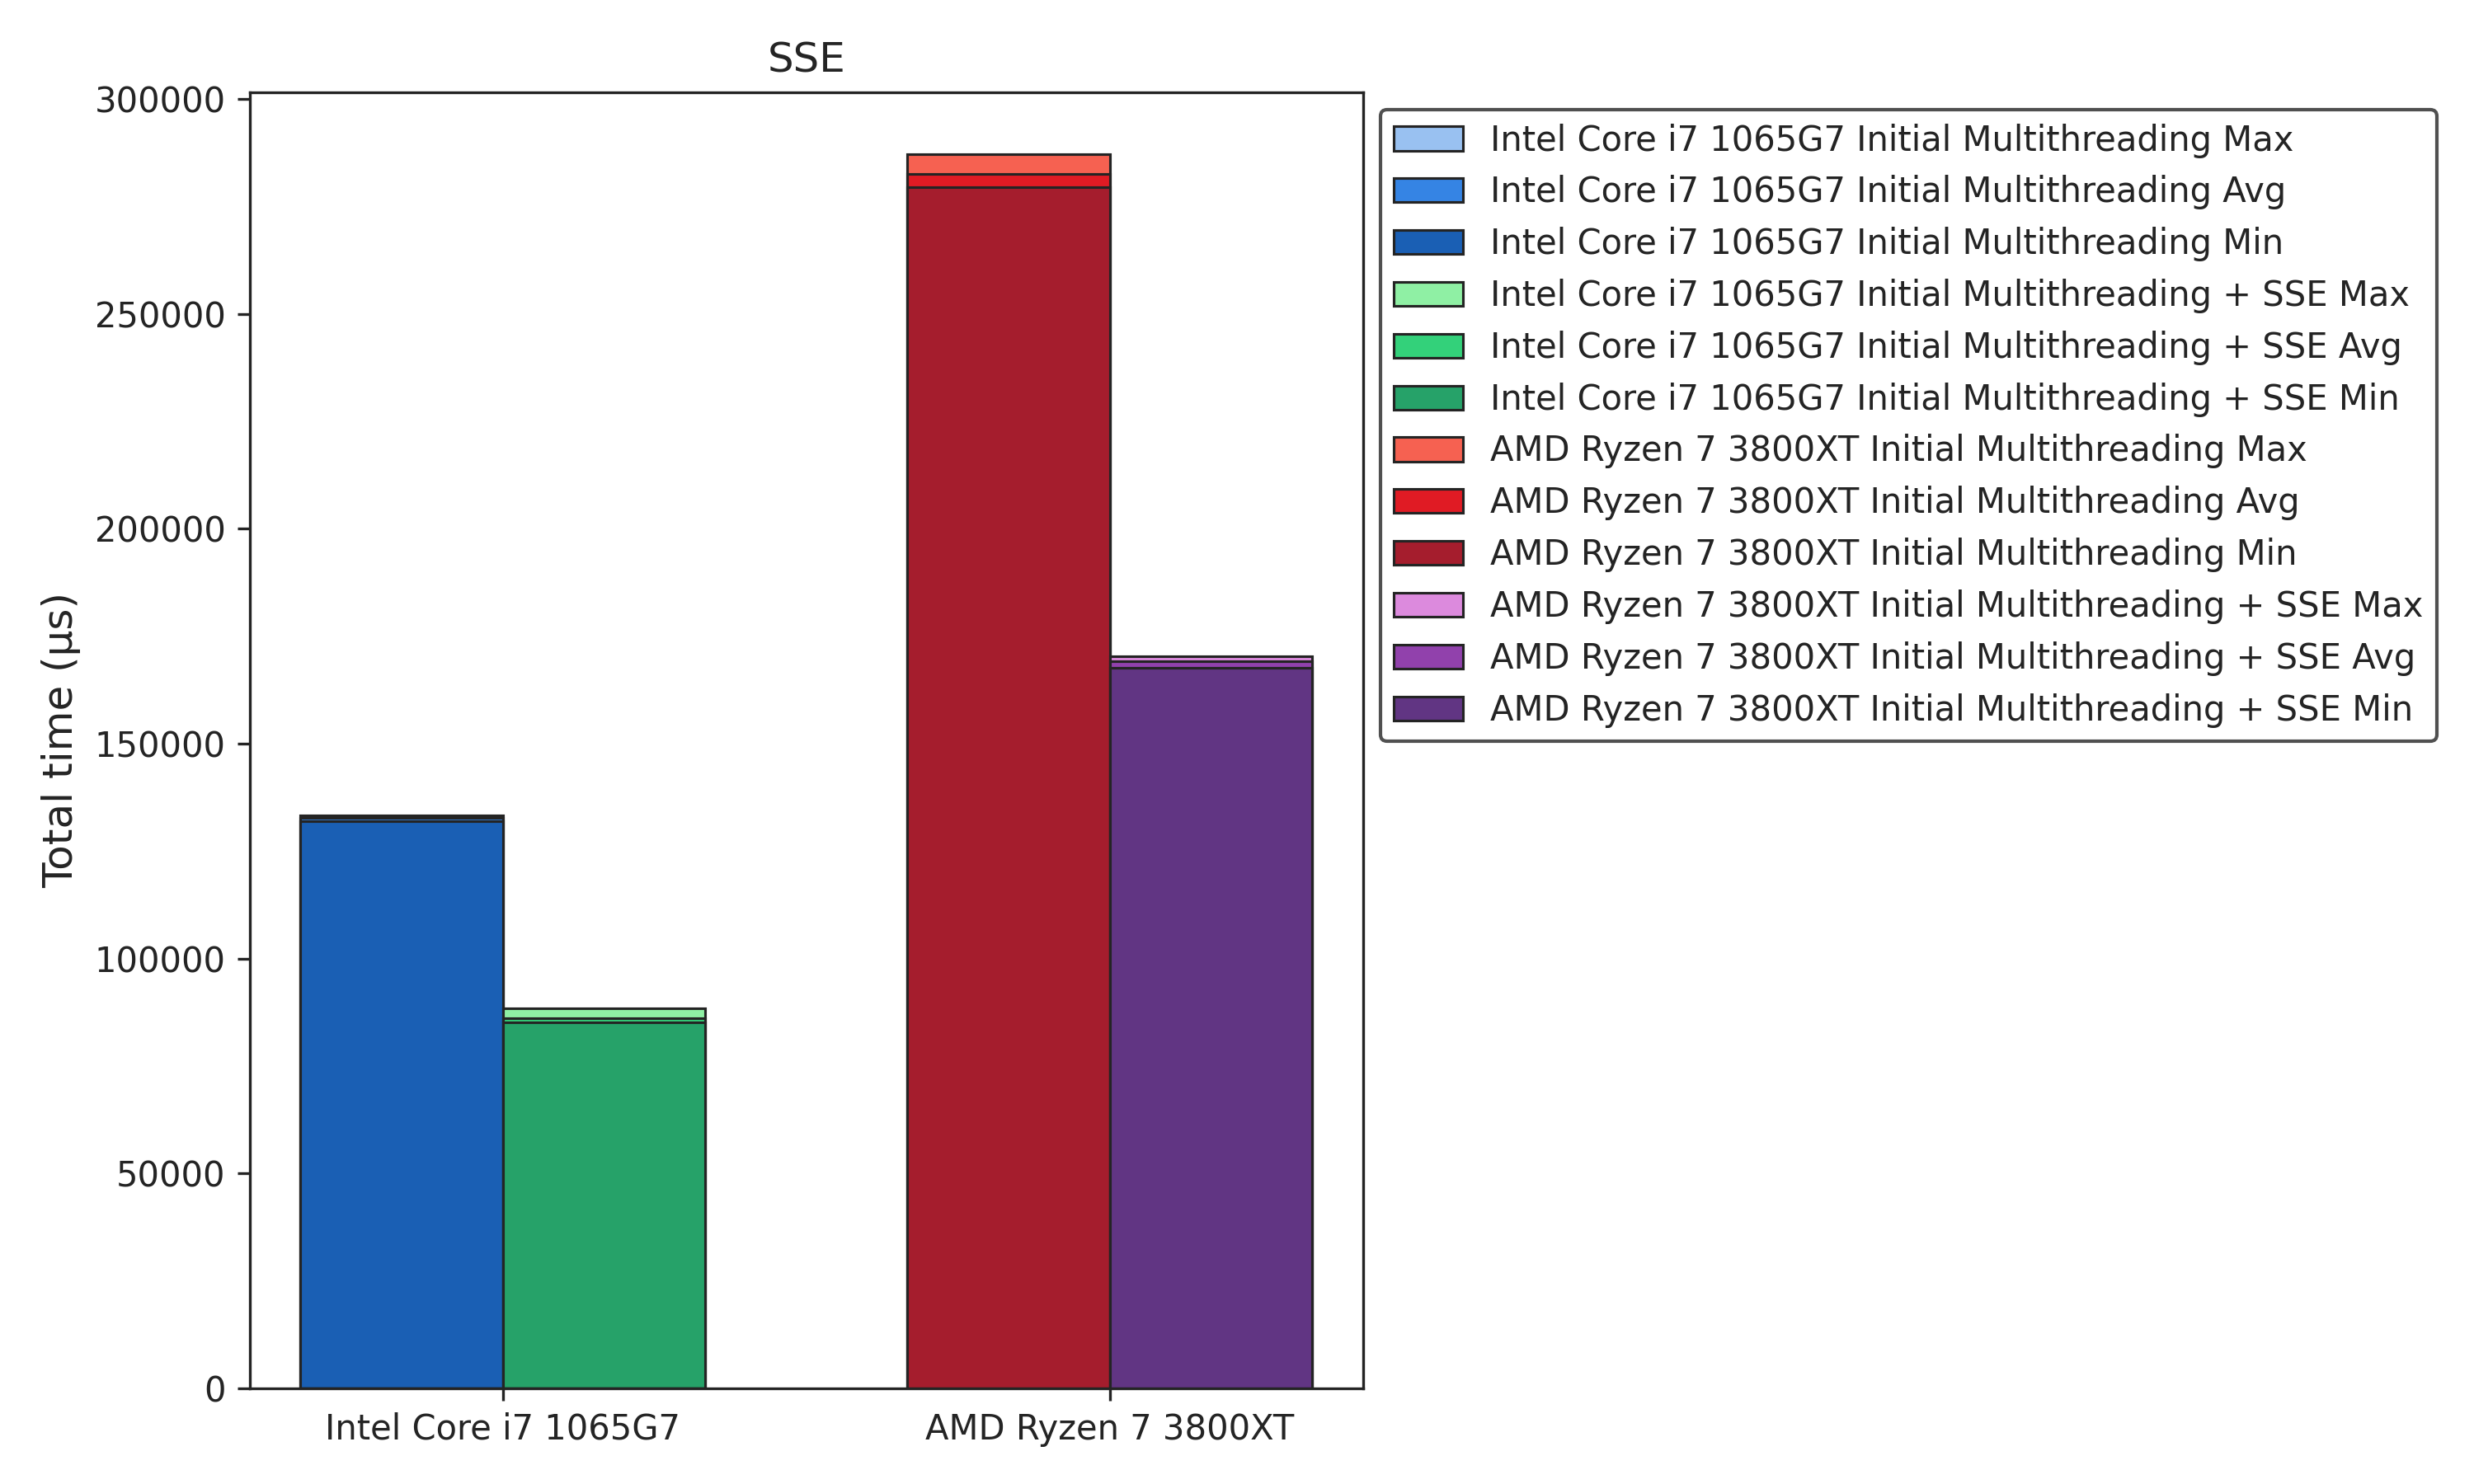
\includegraphics[width=\linewidth]{Graphs/SSE.png}
  \caption{On the MNIST dataset}
 \label{fig:sse_mnist}
\end{subfigure}%
\begin{subfigure}{.5\textwidth}
  \centering
  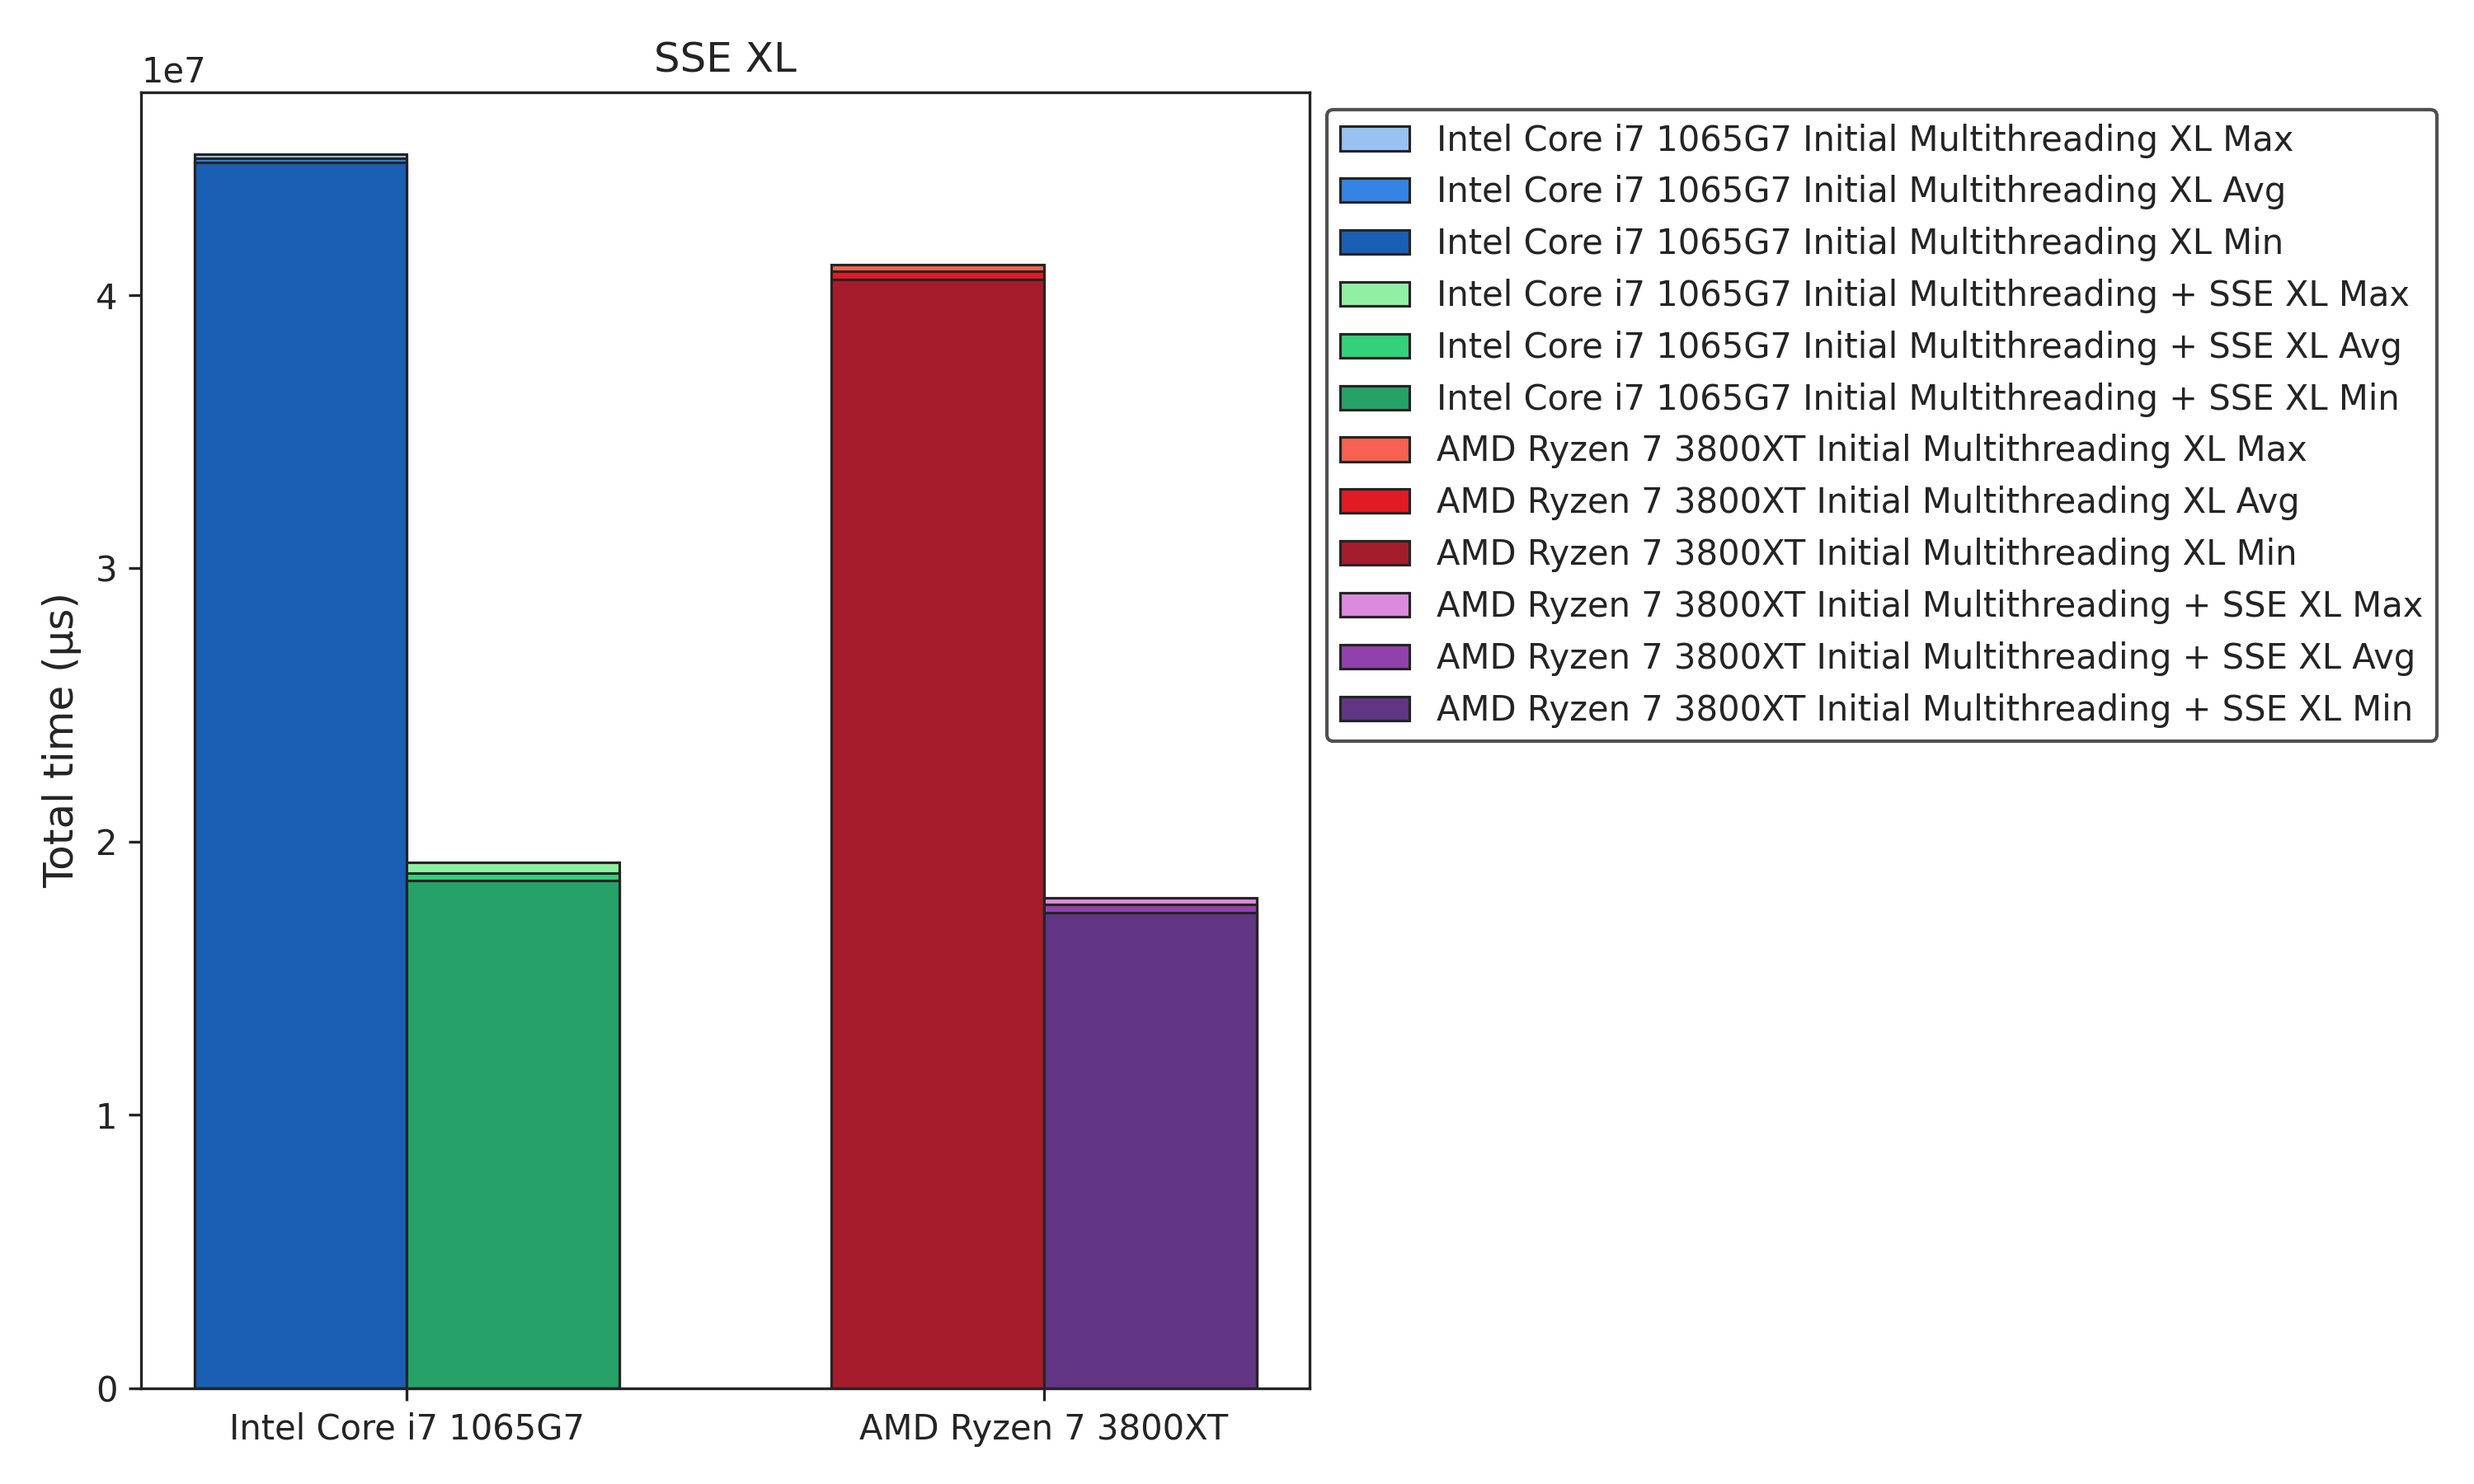
\includegraphics[width=\linewidth]{Graphs/SSE XL.png}
  \caption{On the synthetic XL dataset}
 \label{fig:sse_xl}
\end{subfigure}
\caption{Performance benchmarks of the SSE implementation}
\label{fig:sse}
\end{figure}
\begin{table}[htb!]
\centering
\caption{SSE Implementation\label{tab:sse}}
\begin{tabular}{p{5cm} p{2cm} p{2cm} p{2cm} p{2cm}}
\hline
Benchmark Name & Minimum Value ($\mu$s) & Average Value ($\mu$s) & Maximum Value ($\mu$s) & Standard Deviation \\
\hline
Intel Core i7-1065G7 \\
\hspace{0.5cm}Initial Multithreading \\
\hspace{0.5cm}w/o SSE & 131866.0 & 132756.0 & 133229.0 & 366.1 \\
\hspace{0.5cm}w/ SSE & 85153.0 & 86054.7 & 88349.0 & 1010.9 \\
AMD Ryzen 7 3800XT \\
\hspace{0.5cm}Initial Multithreading \\
\hspace{0.5cm}w/o SSE & 279513.0 & 282589.0 & 287196.0 & 2643.1 \\
\hspace{0.5cm}w/ SSE & 167648.0 & 169152.1 & 170290.0 & 828.8 \\
\hline
Intel Core i7-1065G7 \\
\hspace{0.5cm}Initial Multithreading XL \\
\hspace{0.5cm}w/o SSE & 44870433.0 & 45002714.3 & 45163577.0 & 102509.7 \\
\hspace{0.5cm}w/ SSE & 18579401.0 & 18853792.8 & 19253092.0 & 197720.8 \\
AMD Ryzen 7 3800XT \\
\hspace{0.5cm}Initial Multithreading XL \\
\hspace{0.5cm}w/o SSE & 40573406.0 & 40867988.9 & 41106348.0 & 185968.0 \\
\hspace{0.5cm}w/ SSE & 17411038.0 & 17695422.4 & 17931978.0 & 176916.1 \\
\hline
\end{tabular}
\end{table}
\FloatBarrier

Unfortunately, we do not achieve a fourfold performance improvement. This is likely due to the fact that only four functions benefit from SIMD acceleration, as well as the overhead introduced by memory copying operations. Nevertheless, the performance gain remains substantial and highly encouraging.
\paragraph{Advanced Vector Extensions}
Advanced Vector Extensions (AVX) represent the successor to SSE. AVX doubles the data width to 256 bits and increases the number of registers to 16, named YMM0 to YMM15. In this paper, we use AVX2, an extended version of AVX that is supported by both x86 CPUs and introduces several new operations.\footnote{Introduction to intel advanced vector extensions: \url{https://hpc.llnl.gov/sites/default/files/intelAVXintro.pdf} (Chris Lomont, 2011)}

However, AVX2 still lacks native support for reduction by addition, i.e., summing all elements of a vector in a single instruction. Even worse, it requires breaking down a 256-bit AVX vector into two 128-bit SSE vectors to perform such a reduction. This overhead can potentially result in worse performance compared to SSE.

Listing~\ref{lst:avx2} illustrates how inefficient programming with AVX2 can be, particularly because reduce\_add must be implemented manually.
\begin{lstlisting}[
    caption={AVX2-Based Matrix Multiplication},
    label={lst:avx2},
    language=C++,
    numbers=left,
    numbersep=10pt,
    basicstyle=\fontsize{10}{10}\selectfont,
    breaklines=true,
    postbreak=\mbox{\textcolor{red}{$\hookrightarrow$}\space},
    frame=single,
]
__attribute__((always_inline)) inline void matmul_simd(mt_arg *mt) {
    int CHUNK_SIZE = sizeof(__m256) / sizeof(DATA_TYPE);
    __m256 a, b, c = _mm256_setzero_ps();
    DATA_TYPE sum = 0;
    for(int k = 0; k + CHUNK_SIZE - 1 < ((matrix*)*mt->a)->y; k += CHUNK_SIZE) {
        a = _mm256_loadu_ps(&((matrix*)*mt->a)->m[get_idx(mt->i, k, ((matrix*)*mt->a)->y)]);
        b = _mm256_loadu_ps(&((matrix*)*mt->b)->m[get_idx(mt->j, k, ((matrix*)*mt->b)->y)]);
        c = _mm256_add_ps(_mm256_mul_ps(a, b), c);
    }
    sum += _mm_extract_ps(_mm_hadd_ps(_mm_hadd_ps(_mm_add_ps(_mm256_castps256_ps128(c), _mm256_extractf128_ps(c, 1)), _mm_setzero_ps()), _mm_setzero_ps()), 0);
    for(int k = ((matrix*)*mt->a)->y - (((matrix*)*mt->a)->y % CHUNK_SIZE); k < ((matrix*)*mt->a)->y; k++) {
        sum += ((matrix*)*mt->a)->m[get_idx(mt->i, k, ((matrix*)*mt->a)->y)] * ((matrix*)*mt->b)->m[get_idx(mt->j, k, ((matrix*)*mt->b)->y)];
    }
    (*mt->c)->m[get_idx(mt->i, mt->j, (*mt->c)->y)] = sum;
}
\end{lstlisting}
\paragraph{AVX-512}
AVX-512 doubles the data width once again compared to AVX2, increasing it to 512 bits—hence the name—and expands the number of registers to 32, named ZMM0 through ZMM31. It introduces advanced features such as masked padding and reduction by addition using the powerful and efficient reduce\_add instruction. These enhancements significantly reduce code complexity, lower the likelihood of careless errors, and improve overall performance.

However, AVX-512 is only supported by the Intel processor used in this study. Therefore, we continue to provide an AVX2 implementation as a fallback. The presence of AVX-512 support is detected automatically at compile time, and an appropriate compiler flag is set. This flag is evaluated using conditional compilation, avoiding any runtime overhead due to branching and eliminating the risk of branch mispredictions.

Listing~\ref{lst:avx-512} shows the same matrix multiplication as in Listing~\ref{lst:avx2}, but implemented using AVX-512.
\newpage
\begin{lstlisting}[
    caption={AVX-512-Based Matrix Multiplication},
    label={lst:avx-512},
    language=C++,
    numbers=left,
    numbersep=10pt,
    basicstyle=\fontsize{10}{10}\selectfont,
    breaklines=true,
    postbreak=\mbox{\textcolor{red}{$\hookrightarrow$}\space},
    frame=single,
]
__attribute__((always_inline)) inline void matmul_simd(mt_arg *mt) {
    int CHUNK_SIZE = sizeof(__m512) / sizeof(DATA_TYPE);
    __m512 a, b, c = _mm512_setzero_ps();
    __mmask16 m;
    for(int k = 0; k < ((matrix*)*mt->a)->y; k += CHUNK_SIZE) {
        m = (__mmask16)((1 << (((k + CHUNK_SIZE) <= ((matrix*)*mt->a)->y) ? CHUNK_SIZE : ((matrix*)*mt->a)->y - k)) - 1);
        a = _mm512_maskz_loadu_ps(m, &((matrix*)*mt->a)->m[get_idx(mt->i, k, ((matrix*)*mt->a)->y)]);
        b = _mm512_maskz_loadu_ps(m, &((matrix*)*mt->b)->m[get_idx(mt->j, k, ((matrix*)*mt->b)->y)]);
        c = _mm512_add_ps(_mm512_mul_ps(a, b), c);
    }
    (*mt->c)->m[get_idx(mt->i, mt->j, (*mt->c)->y)] = _mm512_reduce_add_ps(c);
}
\end{lstlisting}

We proceed by examining how AVX impacts the overall performance.
\paragraph{Performance Benchmarks}
The benchmark results are shown in Figure~\ref{fig:avx}, with the corresponding values listed in Table~\ref{tab:avx}. The average performance of all CPUs on the MNIST dataset improves by 10.5\%. The average performance of the Intel Core i7-1065G7 improves by 24.7\% and the AMD Ryzen 7 3800XT improves by 3.1\%. The average performance of all CPUs on the synthetic XL dataset improves by 1.2\%. The Intel Core i7-1065G7 improves by 1.9\% and the AMD Ryzen 7 3800XT improves by 0.3\%.
\begin{figure}[htb!]
\centering
\begin{subfigure}{.5\textwidth}
  \centering
  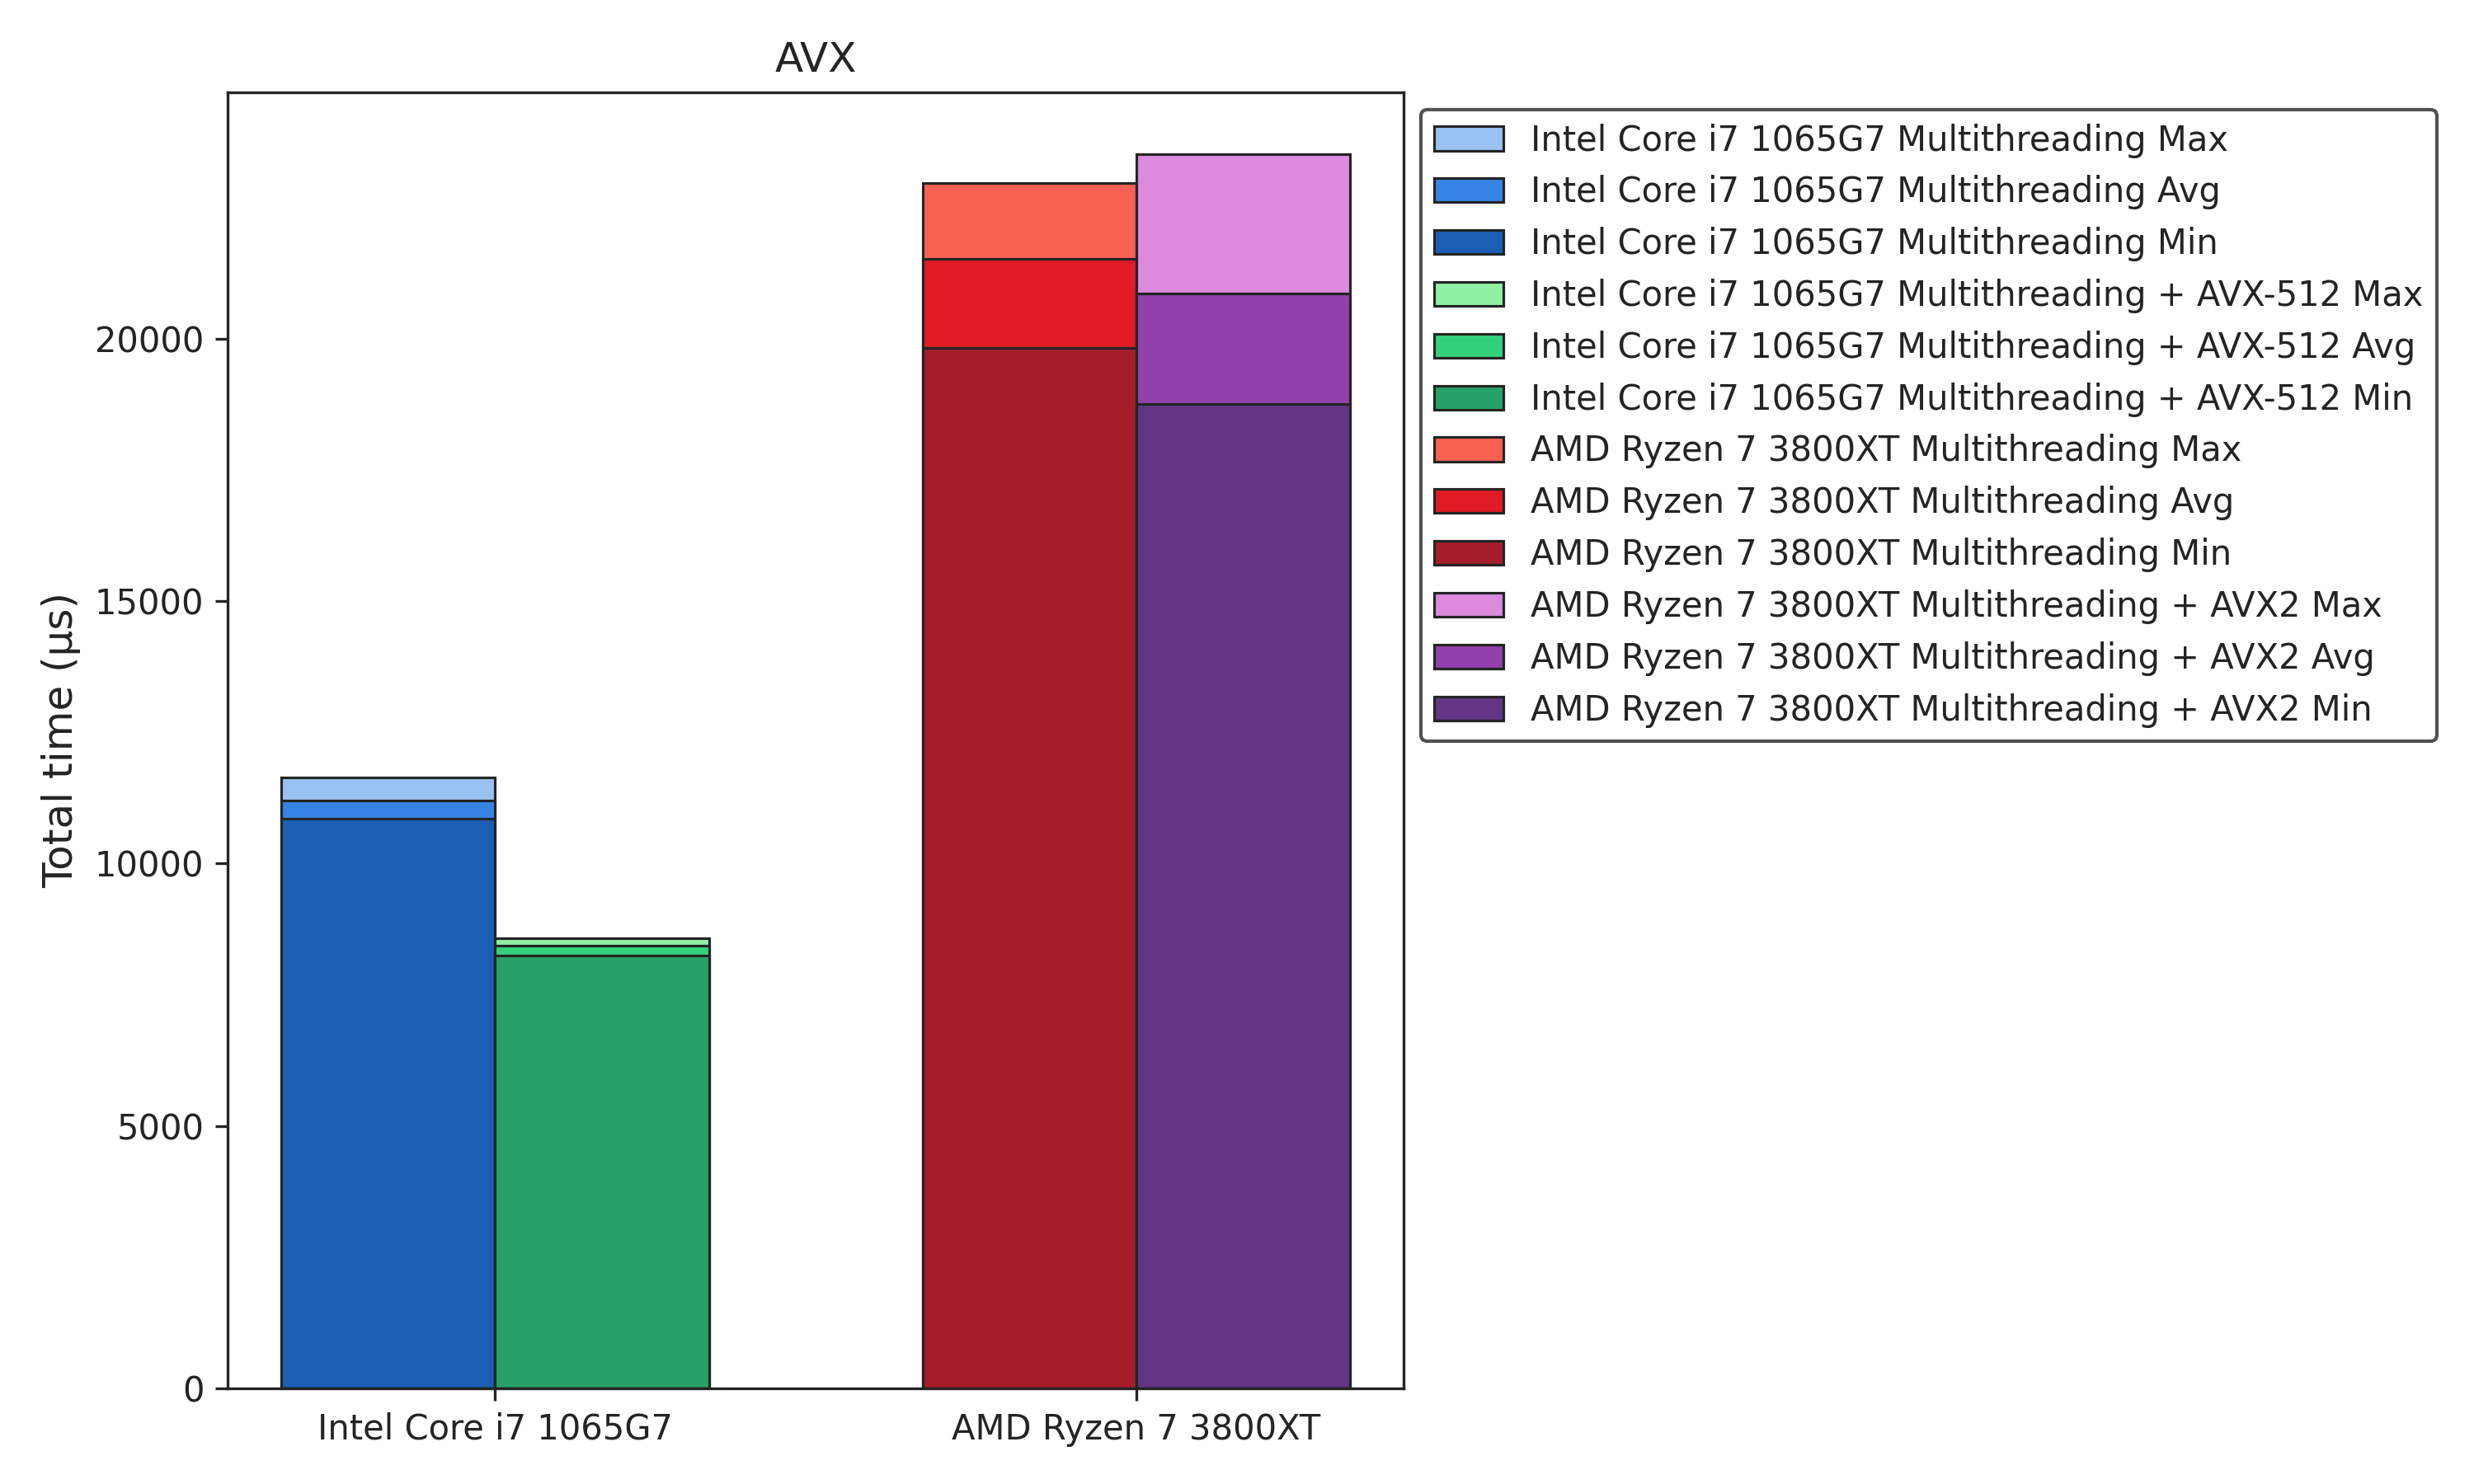
\includegraphics[width=\linewidth]{Graphs/AVX.png}
  \caption{On the MNIST dataset}
 \label{fig:avx_mnist}
\end{subfigure}%
\begin{subfigure}{.5\textwidth}
  \centering
  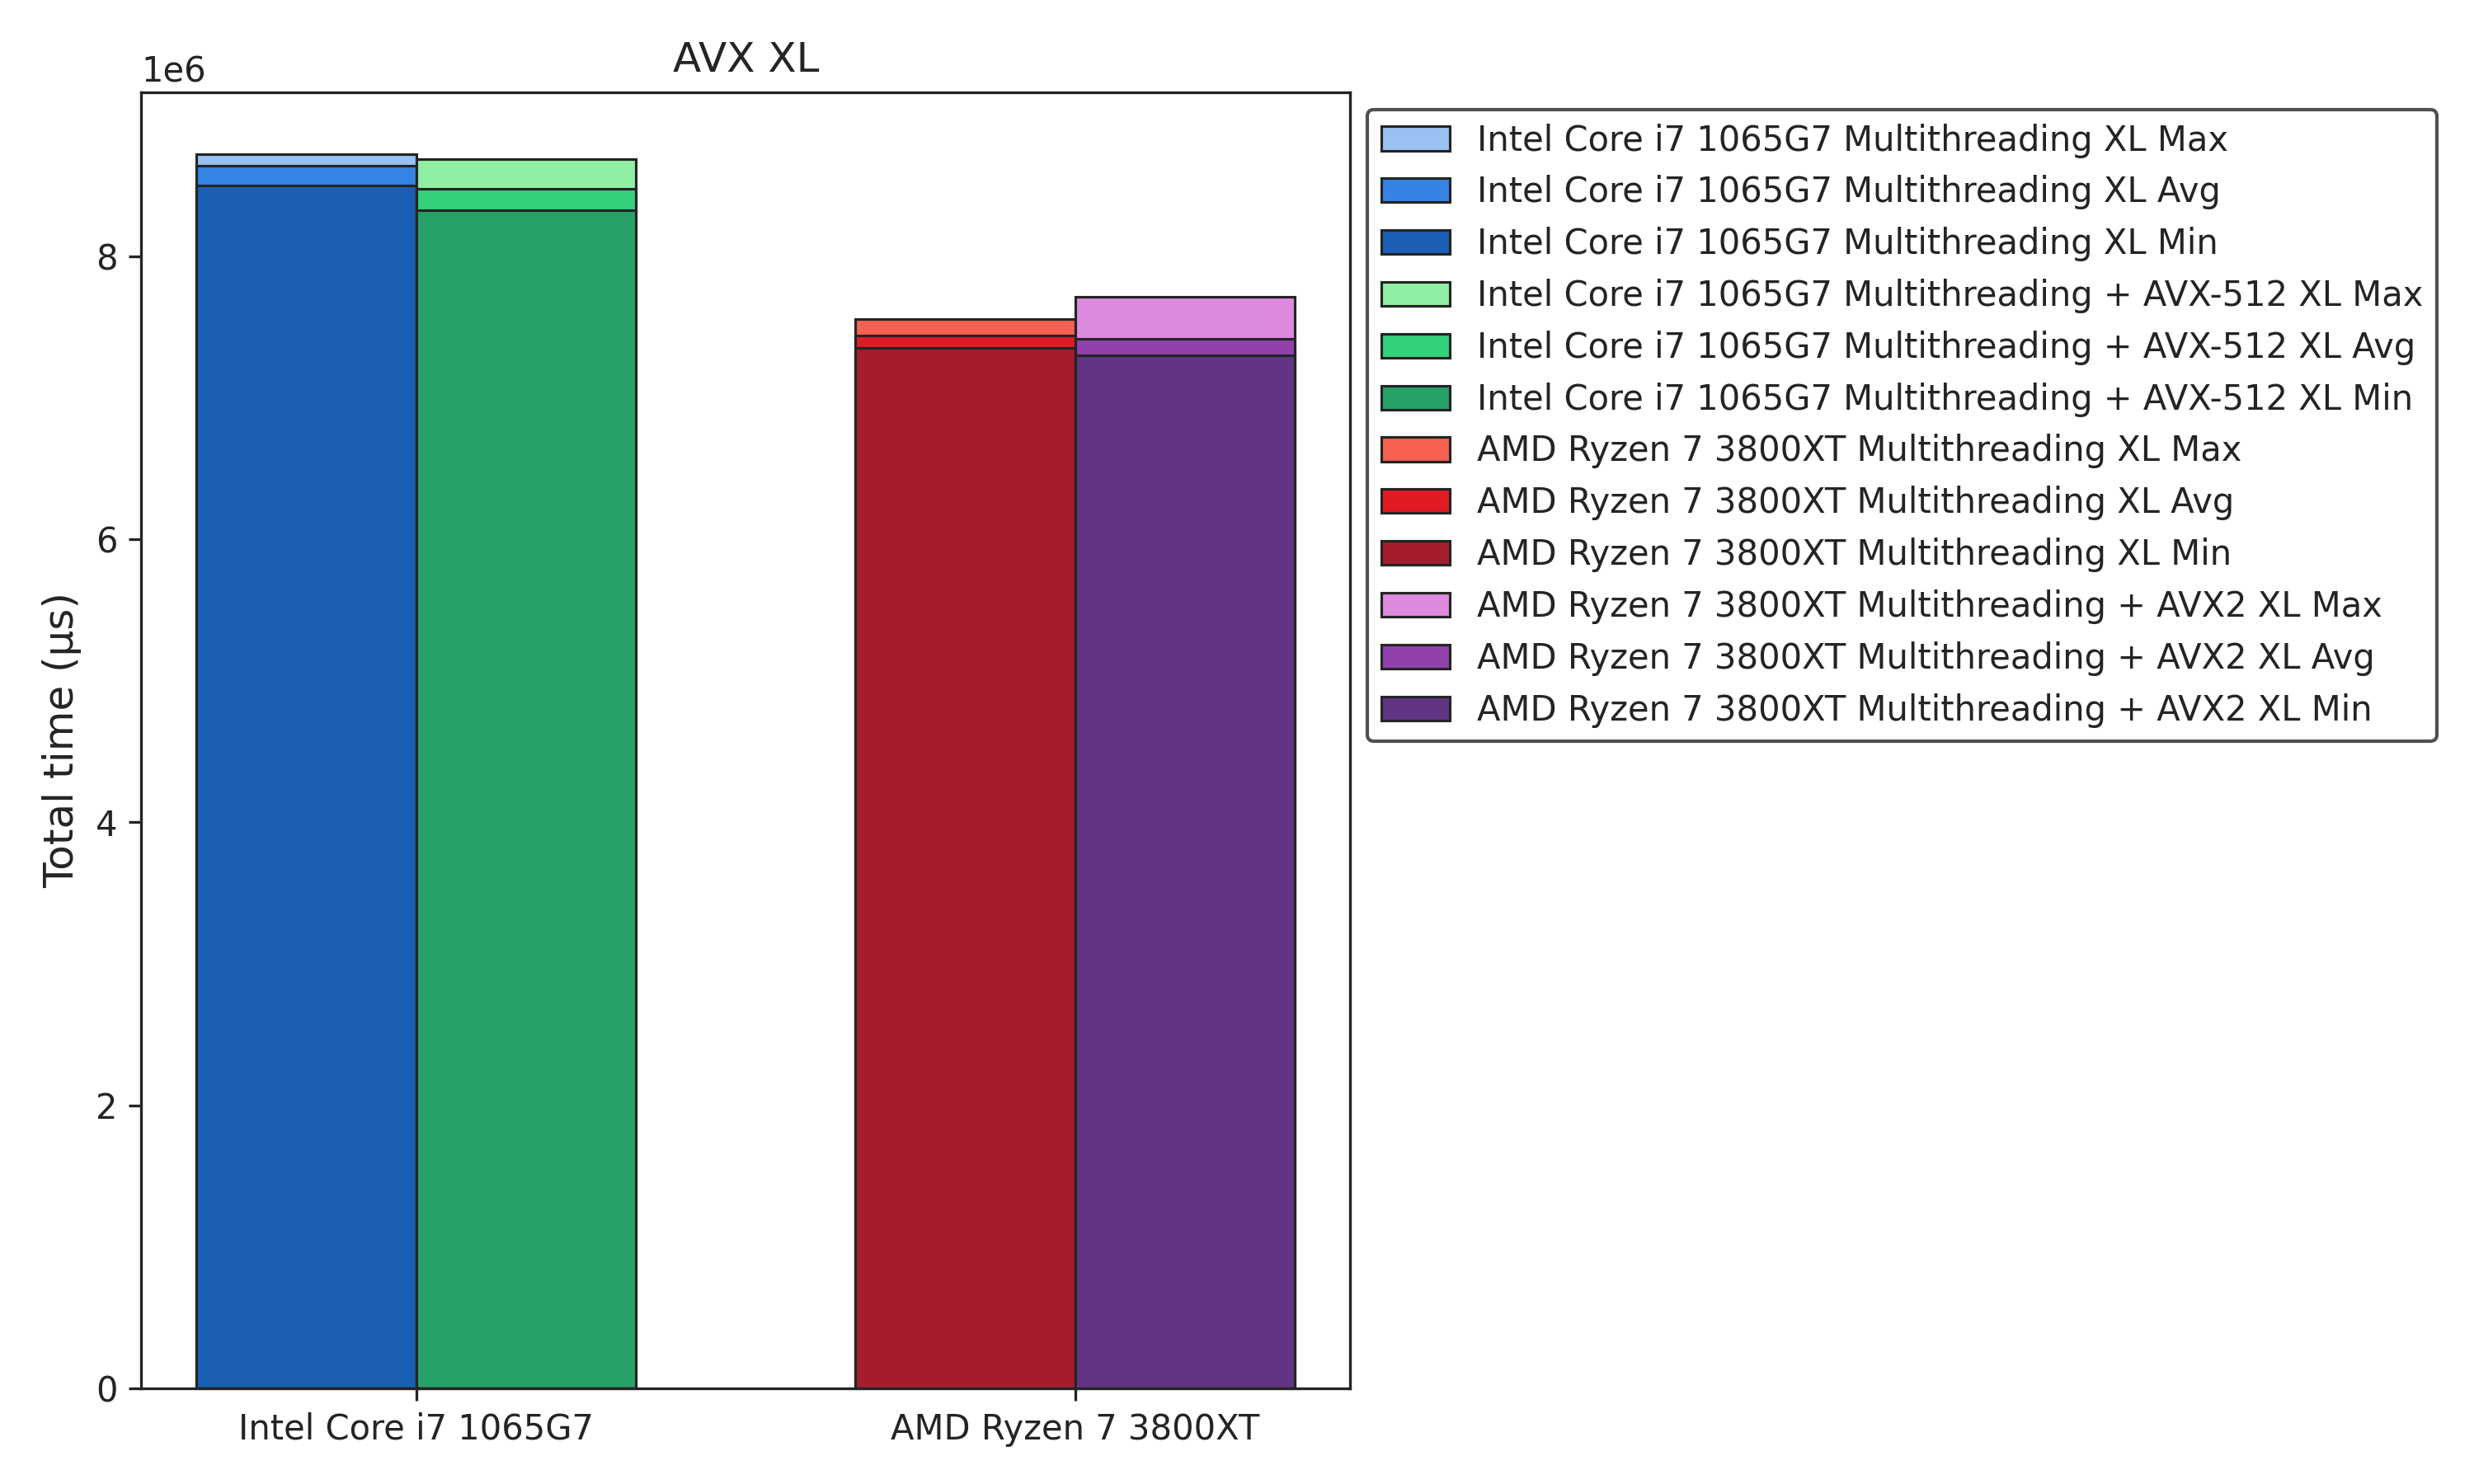
\includegraphics[width=\linewidth]{Graphs/AVX XL.png}
  \caption{On the synthetic XL dataset}
 \label{fig:avx_xl}
\end{subfigure}
\caption{Performance benchmarks of the AVX implementation}
\label{fig:avx}
\end{figure}
\begin{table}[htb!]
\centering
\caption{AVX Implementation\label{tab:avx}}
\begin{tabular}{p{5cm} p{2cm} p{2cm} p{2cm} p{2cm}}
\hline
Benchmark Name & Minimum Value ($\mu$s) & Average Value ($\mu$s) & Maximum Value ($\mu$s) & Standard Deviation \\
\hline
Intel Core i7-1065G7 \\
\hspace{0.5cm}Multithreading \\
\hspace{0.5cm}w/o AVX-512 & 10851.0 & 11205.8 & 11643.0 & 231.2 \\
\hspace{0.5cm}w/ AVX-512 & 8249.0 & 8437.5 & 8580.0 & 114.8 \\
AMD Ryzen 7 3800XT \\
\hspace{0.5cm}Multithreading \\
\hspace{0.5cm}w/o AVX2 & 19826.0 & 21530.2 & 22967.0 & 824.8 \\
\hspace{0.5cm}w/ AVX2 & 18756.0 & 20865.3 & 23525.0 & 1207.6 \\
\hline
Intel Core i7-1065G7 \\
\hspace{0.5cm}Multithreading XL \\
\hspace{0.5cm}w/o AVX-512 & 8500620.0 & 8636423.7 & 8721267.0 & 75104.0 \\
\hspace{0.5cm}w/ AVX-512 & 8323409.0 & 8475420.5 & 8682675.0 & 116904.7 \\
AMD Ryzen 7 3800XT \\
\hspace{0.5cm}Multithreading XL \\
\hspace{0.5cm}w/o AVX2 & 7352356.0 & 7438704.9 & 7552378.0 & 63658.1 \\
\hspace{0.5cm}w/ AVX2 & 7296720.0 & 7414562.6 & 7711956.0 & 126810.9 \\
\hline
\end{tabular}
\end{table}
\FloatBarrier

As expected, AVX2 offers only marginal improvements, since the advantages of SIMD are significantly limited by the extensive overhead introduced by our custom, SSE-based reduction-by-addition implementation. In contrast, AVX-512 shows a much more substantial performance gain, which is a very positive result. However, AVX-512 also faces limitations in this comparison, as we use the optimized version of our multithreading implementation. This version creates the maximum number of threads, each utilizing multiple AVX registers. As a result, the demand for vector registers exceeds the available capacity, leading to a bottleneck. Nevertheless, the transition from no SIMD, through SSE, and ultimately to AVX proves to be clearly worthwhile and will definitely serve as the foundation for future optimizations.
\subsection{Quantization}\label{sec:quantization}
\subsubsection{Overview of Quantization}
Another optimization opportunity we identified lies in quantization. Quantization refers to the process of reducing the precision of computations in order to improve efficiency and decrease memory usage. Within our framework, we reduced the input values from float32 to int8 to lower memory consumption and increase processing speed. Despite the reduced precision, the prediction accuracy was largely preserved, with only a 5\% to 8\% loss. This is due to the fact that while int8 can represent a smaller range of values compared to float32, it still provides sufficient resolution for inputs such as weights and extracted image features. Additionally, we used int32 as the data type for intermediate computations to maintain numerical precision and avoid overflows. This adjustment reduces the overall model size and accelerates computation without significantly affecting model performance.

The SIMD code was extended to support quantization, enabling AVX2, AVX-512, and Arm Neon to handle various data types. As previously mentioned, however, AMX does not support the int8 data type, which prevented our input values from being processed in this case. The implications of this limitation are discussed in more detail in the following sections.
\subsubsection{Memory Usage}
Adjusting the input values led to a reduction in model size of approximately 15\% (see Table~\ref{tab:quant_mem_red}). Nonetheless, the overall memory savings fell short of expectations due to the substantial and irreducible memory overhead introduced by the multithreading instance

\begin{table}[htb!]
\centering
\caption{Quantization Memory Reduction\label{tab:quant_mem_red}}
\begin{tabular}{p{3cm} p{2cm}}
\hline
Benchmark Name & Bytes \\
\hline
NO\_SIMD & 2.409.961\\
\hline
NO\_SIMD\_INT & 2.050.771 \\
\hline
\end{tabular}
\end{table}
\FloatBarrier
\subsubsection{Performance Benchmarks}
The benchmark results are shown in Figure~\ref{fig:quantization}, with the corresponding values listed in Table~\ref{tab:quantization}. The average performance of all CPUs on the MNIST dataset decreases by 0.4\%. The average performance of the Intel Core i7-1065G7 decreases by 2.5\%, the Apple M3 Pro 11-Core decreases by 0.9\%, and the AMD Ryzen 7 3800XT improves by 1.0\%. The average performance of all CPUs on the synthetic XL dataset improves by 0.7\%. The Intel Core i7-1065G7 improves by 1.0\%, the Apple M3 Pro 11-Core decreases by 5.4\%, and the AMD Ryzen 7 3800XT improves by 2.9\%.

\begin{figure}[htb!]
\centering
\begin{subfigure}{.5\textwidth}
  \centering
  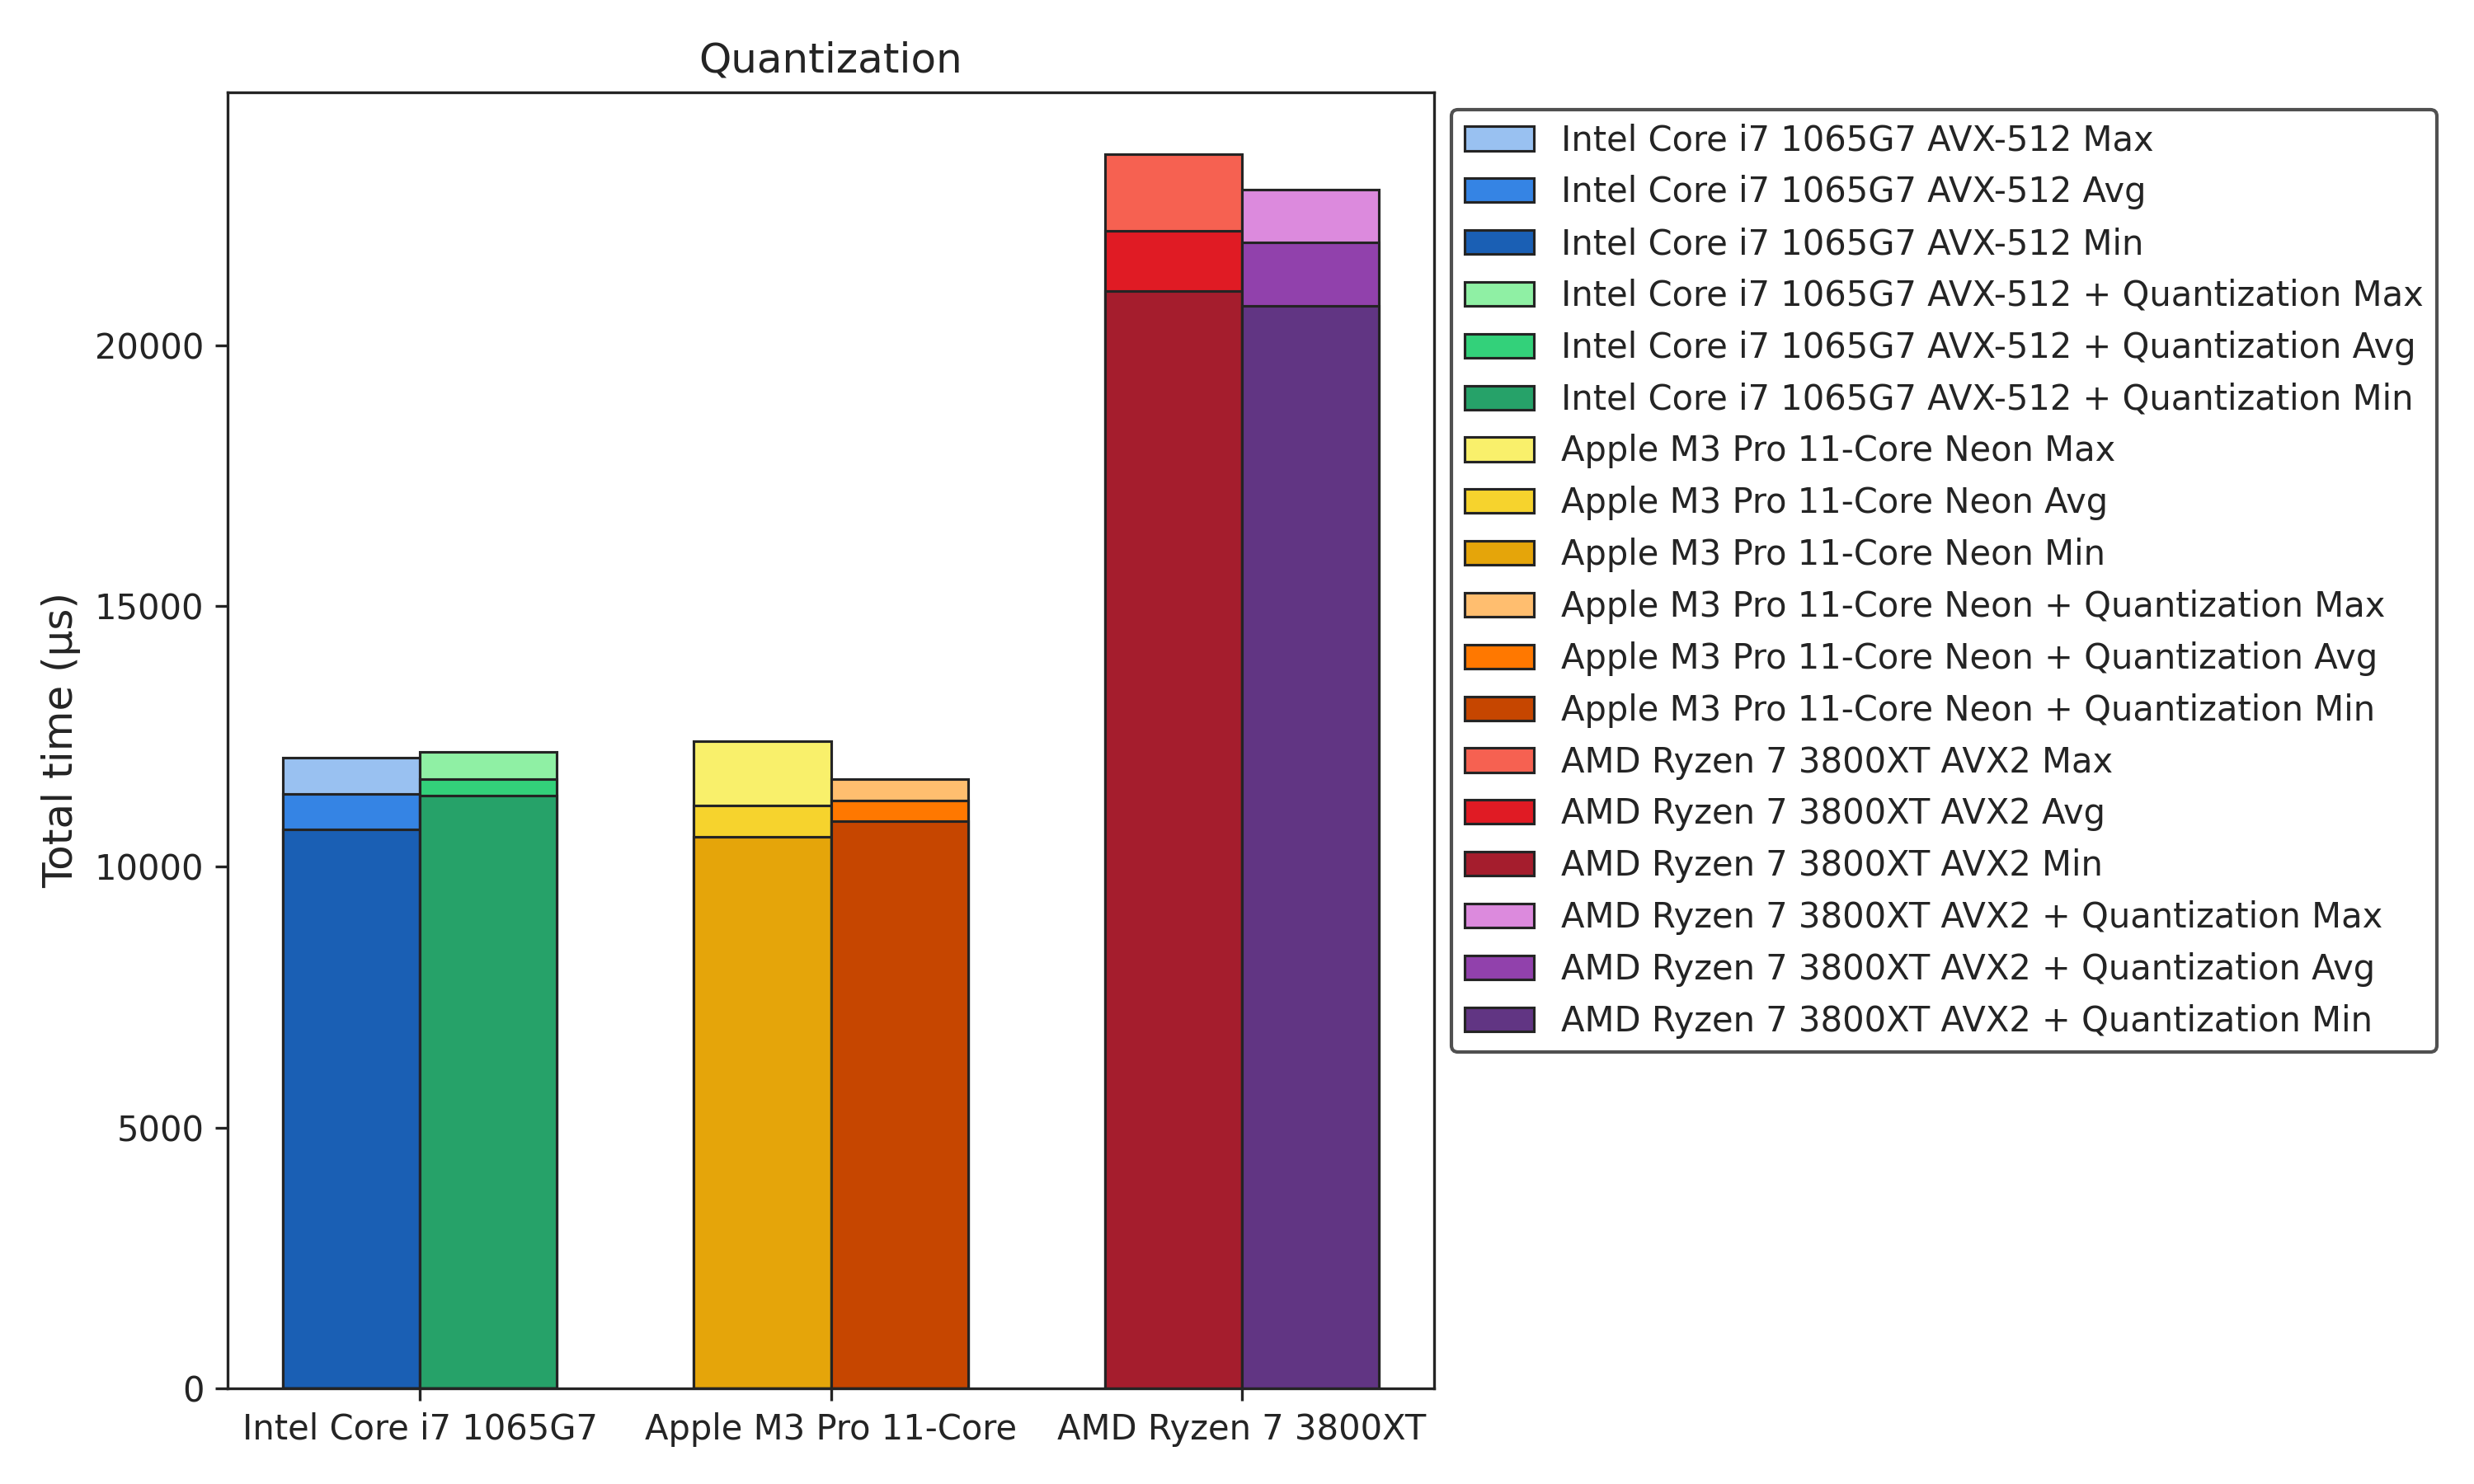
\includegraphics[width=\linewidth]{Graphs/Quantization.png}
  \caption{On the MNIST dataset}
 \label{fig:quant_mnist}
\end{subfigure}%
\begin{subfigure}{.5\textwidth}
  \centering
  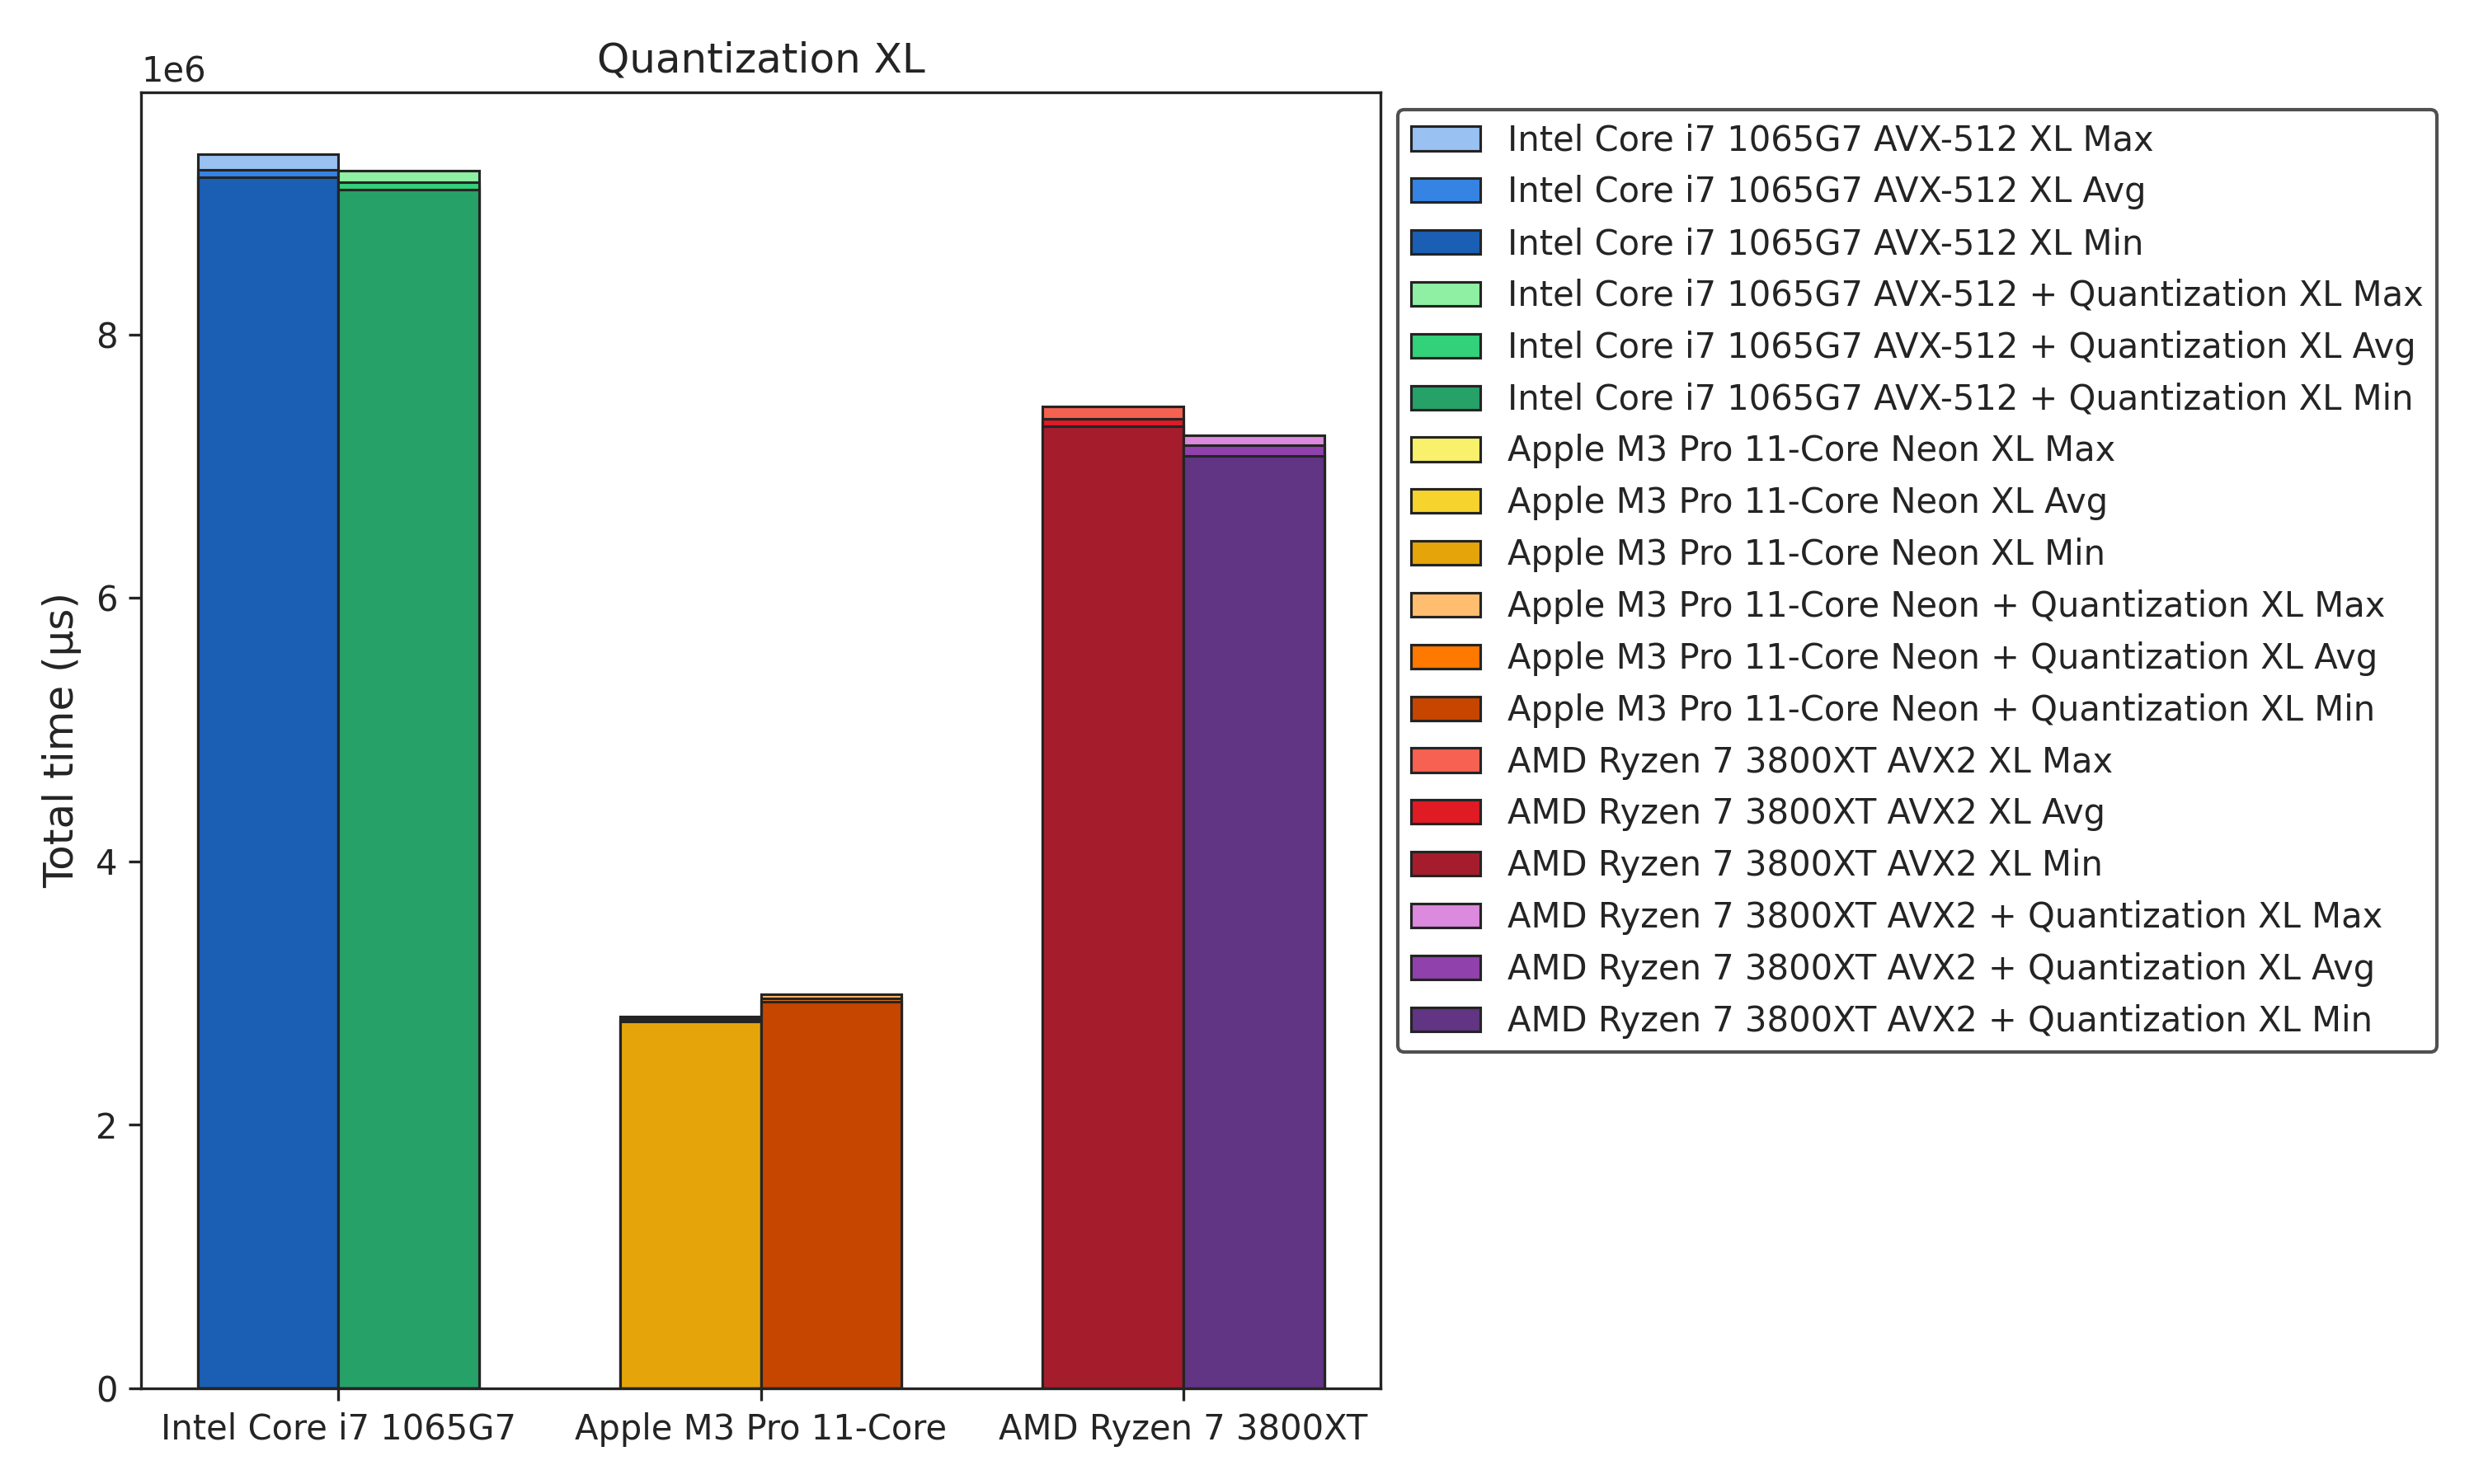
\includegraphics[width=\linewidth]{Graphs/Quantization XL.png}
  \caption{On the synthetic XXL dataset}
 \label{fig:quant_xl}
\end{subfigure}
\caption{Performance benchmarks of Quantization}
\label{fig:quantization}
\end{figure}
\begin{table}[htb!]
\centering

\caption{Quantization\label{tab:quantization}}
\begin{tabular}{p{5.5cm} p{2cm} p{2cm} p{2cm} p{2cm}}
\hline
Benchmark Name & Minimum Value ($\mu$s) & Average Value ($\mu$s) & Maximum Value ($\mu$s) & Standard Deviation \\
\hline
Intel Core i7-1065G7 \\
\hspace{0.5cm}AVX-512 & 10725.0 & 11398.8 & 12087.0 & 417.5 \\
\hspace{0.5cm}AVX-512 + Quantization & 11366.0 & 11687.6 & 12211.0 & 260.0 \\
Apple M3 Pro 11-Core \\
\hspace{0.5cm}Neon & 10575.0 & 11170.5 & 12407.0 & 618.4 \\
\hspace{0.5cm}Neon + Quantization & 10879.0 & 11275.8 & 11688.0 & 197.5 \\
AMD Ryzen 7 3800XT \\
\hspace{0.5cm}AVX2 & 21050.0 & 22202.5 & 23671.0 & 747.3 \\
\hspace{0.5cm}AVX2 + Quantization & 20760.0 & 21984.3 & 22984.0 & 603.6 \\
\hline
Intel Core i7-1065G7 \\
\hspace{0.5cm}AVX-512 XL & 9195229.0 & 9246640.6 & 9369463.0 & 52836.7 \\
\hspace{0.5cm}AVX-512 + Quantization XL & 9098525.0 & 9157208.8 & 9246307.0 & 41926.1 \\
Apple M3 Pro 11-Core \\
\hspace{0.5cm}Neon XL & 2783871.0 & 2802165.9 & 2824752.0 & 13541.5 \\
\hspace{0.5cm}Neon + Quantization XL & 2932706.0 & 2962501.3 & 2989630.0 & 18044.8 \\
AMD Ryzen 7 3800XT \\
\hspace{0.5cm}AVX2 XL & 7302691.0 & 7361732.2 & 7450227.0 & 50234.5 \\
\hspace{0.5cm}AVX2 + Quantization XL & 7077489.0 & 7156612.6 & 7233151.0 & 50051.6 \\
\hline
\end{tabular}
\end{table}
\FloatBarrier

The benchmarks indicate that quantization has only a marginal effect on performance, both for the MNIST dataset and the synthetic XL test. A key factor contributing to the nearly unchanged execution time is type casting. Since the input values are stored as int8 while intermediate computations are performed in int32, values must be cast between types—most notably from int8 to int32. This casting introduces a non-negligible overhead, especially in the context of SIMD-based execution, where uniformity of data types is crucial for optimal throughput.

Both AVX and Arm Neon are primarily optimized for floating-point operations, a design choice rooted in their original application domains such as scientific computing, media processing, and signal processing. As a result, SIMD pipelines on both architectures typically provide better throughput and latency for float32 and float64 operations compared to integer arithmetic—particularly when dealing with non-uniform or mixed datatypes. This hardware-level optimization further explains why quantized models, despite reduced memory and arithmetic precision (e.g., int8), do not always translate into significant performance gains: internally, many operations are either promoted to int32 or incur overhead due to type conversions, offsetting the theoretical advantages of quantization. Optimizing for integer performance often requires architecture-specific tuning and careful control over casting and alignment.\footnote{ARM NEON optimization: \url{https://community.arm.com/arm-community-blogs/b/operating-systems-blog/posts/arm-neon-optimization} (accessed April 19, 2025).}$^{,}$\footnote{Avoiding Mixed Data Type Arithmetic Expressions: \url{https://www.intel.com/content/www/us/en/docs/cpp-compiler/developer-guide-reference/2021-9/handle-floating-point-array-operations-loop-body.html} (accessed April 19, 2025).}
\subsection{Other Optimizations}\label{sec:other-optimizations}
This chapter consolidates a series of smaller optimizations implemented throughout the development process.

First, all functions previously allocated new memory for the result matrix upon every invocation. These memory allocations involve costly system calls and unnecessarily increase the memory footprint, especially given that multiple images are typically processed in sequence. To address this, we introduce an optional third parameter to each function in our custom TensorFlow module. If this parameter is set to null, the function behaves as before; otherwise, it writes the output directly to the provided pointer without allocating new memory. This modification enables us to move all memory allocations and deallocations outside of performance-critical loops, thereby improving execution speed and reducing memory consumption.

Next, we eliminate redundant transpose operations on the fc\_bias and fc\_weights matrices. These operations, repeated in every iteration and not meaningfully parallelizable due to the matrices' dimensions, are now avoided by pre-transposing the constant input matrices and storing them in this format within the input text file. This change saves a significant number of function calls during runtime.

We also merge the final transpose operation with the flattening step. The flatten function now directly allocates a transposed result matrix and writes the correctly ordered values to it. This prevents the need for a subsequent reordering step, further enhancing performance.

At this stage, a number of outdated or unused functions have accumulated. We remove these to reduce code complexity and decrease binary size. Additionally, we employ Clang-specific and C++11 features to minimize boilerplate code and extend functionality.

The Chapter~\ref{sec:gpu-based-optimizations} addresses GPU-based optimizations using CUDA. However, our current framework is not yet fully designed for CUDA integration. Apart from the multithreading module, which we port to a C++ class in Section~\ref{subsec:optimized-implementation}, the remaining components are still written in C. Our initial intention to use extern "C" proves too complex and ultimately non-functional. As a result, we port the entire framework to C++, rewriting or refactoring large portions in the process.

Given that CUDA is optimized for flat arrays, we adapt our matrix structure accordingly. This change also improves cache utilization. For element addressing, we introduce the helper function get\_idx, which calculates flat indices efficiently.

One of the most impactful optimizations involves applying the always\_inline attribute to inline all functions, significantly reducing overhead. We validate this optimization using the profiling tool gprof, which confirms that, among other things, thousands of calls to get\_idx are effectively eliminated.\footnote{Understanding and Exploiting Optimal Function Inlining: \url{https://www.pure.ed.ac.uk/ws/portalfiles/portal/261328587/Understanding_and_Exploiting_THEODORIDIS_DOA15112021_AFV.pdf} (Theodoridis, Theodoros, Tobias Grosser, and Zhendong Su, 2022)}

Finally, we modularize all disjoint optimizations. The system now offers three distinct run functions—one each for CUDA, OpenMP, and multithreading—greatly improving logical separation and simplifying maintenance.
\subsection{Inital vs. Final Implementation}\label{sec:inital-vs-final-implementation}
The benchmark results are shown in Figure~\ref{fig:initial_vs_final}, with the corresponding values listed in Table~\ref{tab:initial_vs_final}. The average performance of all CPUs on the MNIST dataset improves by 59.6\%. The average performance of the Intel Core i7-1065G7 improves by 74.0\%, the Apple M3 Pro 11-Core improves by 59.6\%, and the AMD Ryzen 7 3800XT improves by 43.5\%. The average performance of all CPUs on the synthetic XL dataset improves by 85.4\%. The Intel Core i7-1065G7 improves by 82.9\%, the Apple M3 Pro 11-Core improves by 90.4\%, and the AMD Ryzen 7 3800XT improves by 85.3\%.
\begin{figure}[htb!]
\centering
\begin{subfigure}{.5\textwidth}
  \centering
  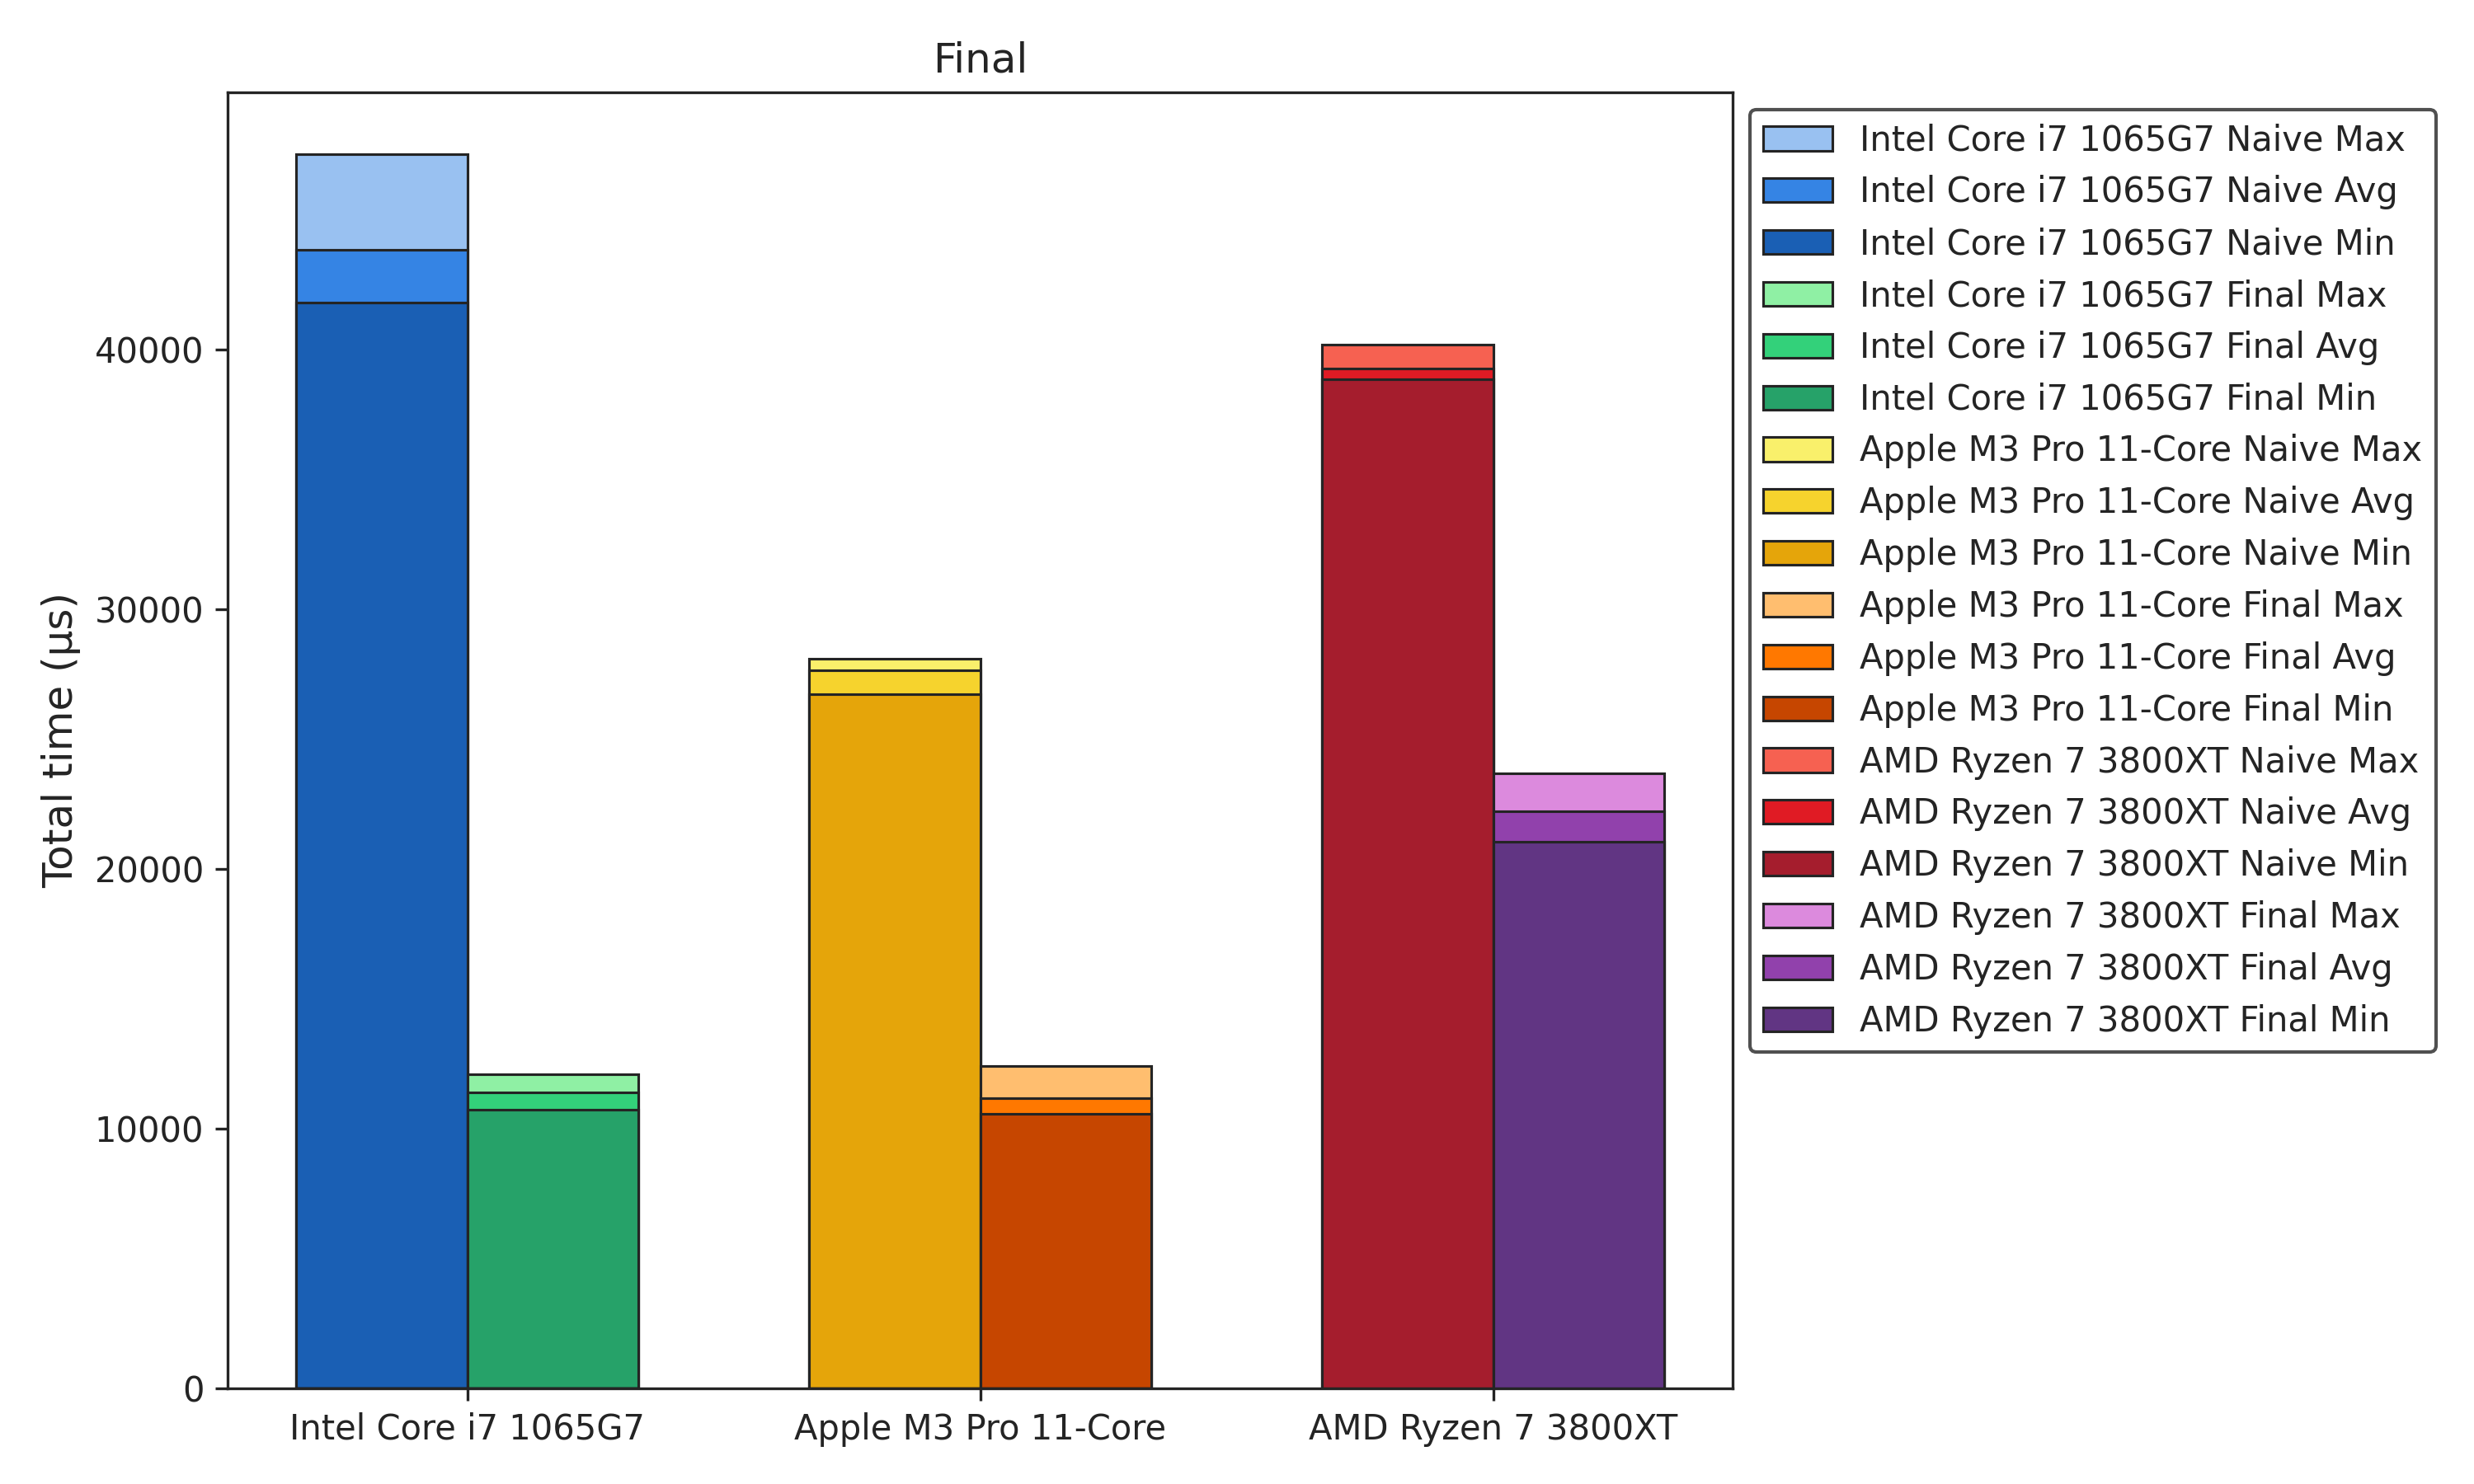
\includegraphics[width=\linewidth]{Graphs/Final.png}
  \caption{On the MNIST dataset}
 \label{fig:initial_vs_final_mnist}
\end{subfigure}%
\begin{subfigure}{.5\textwidth}
  \centering
  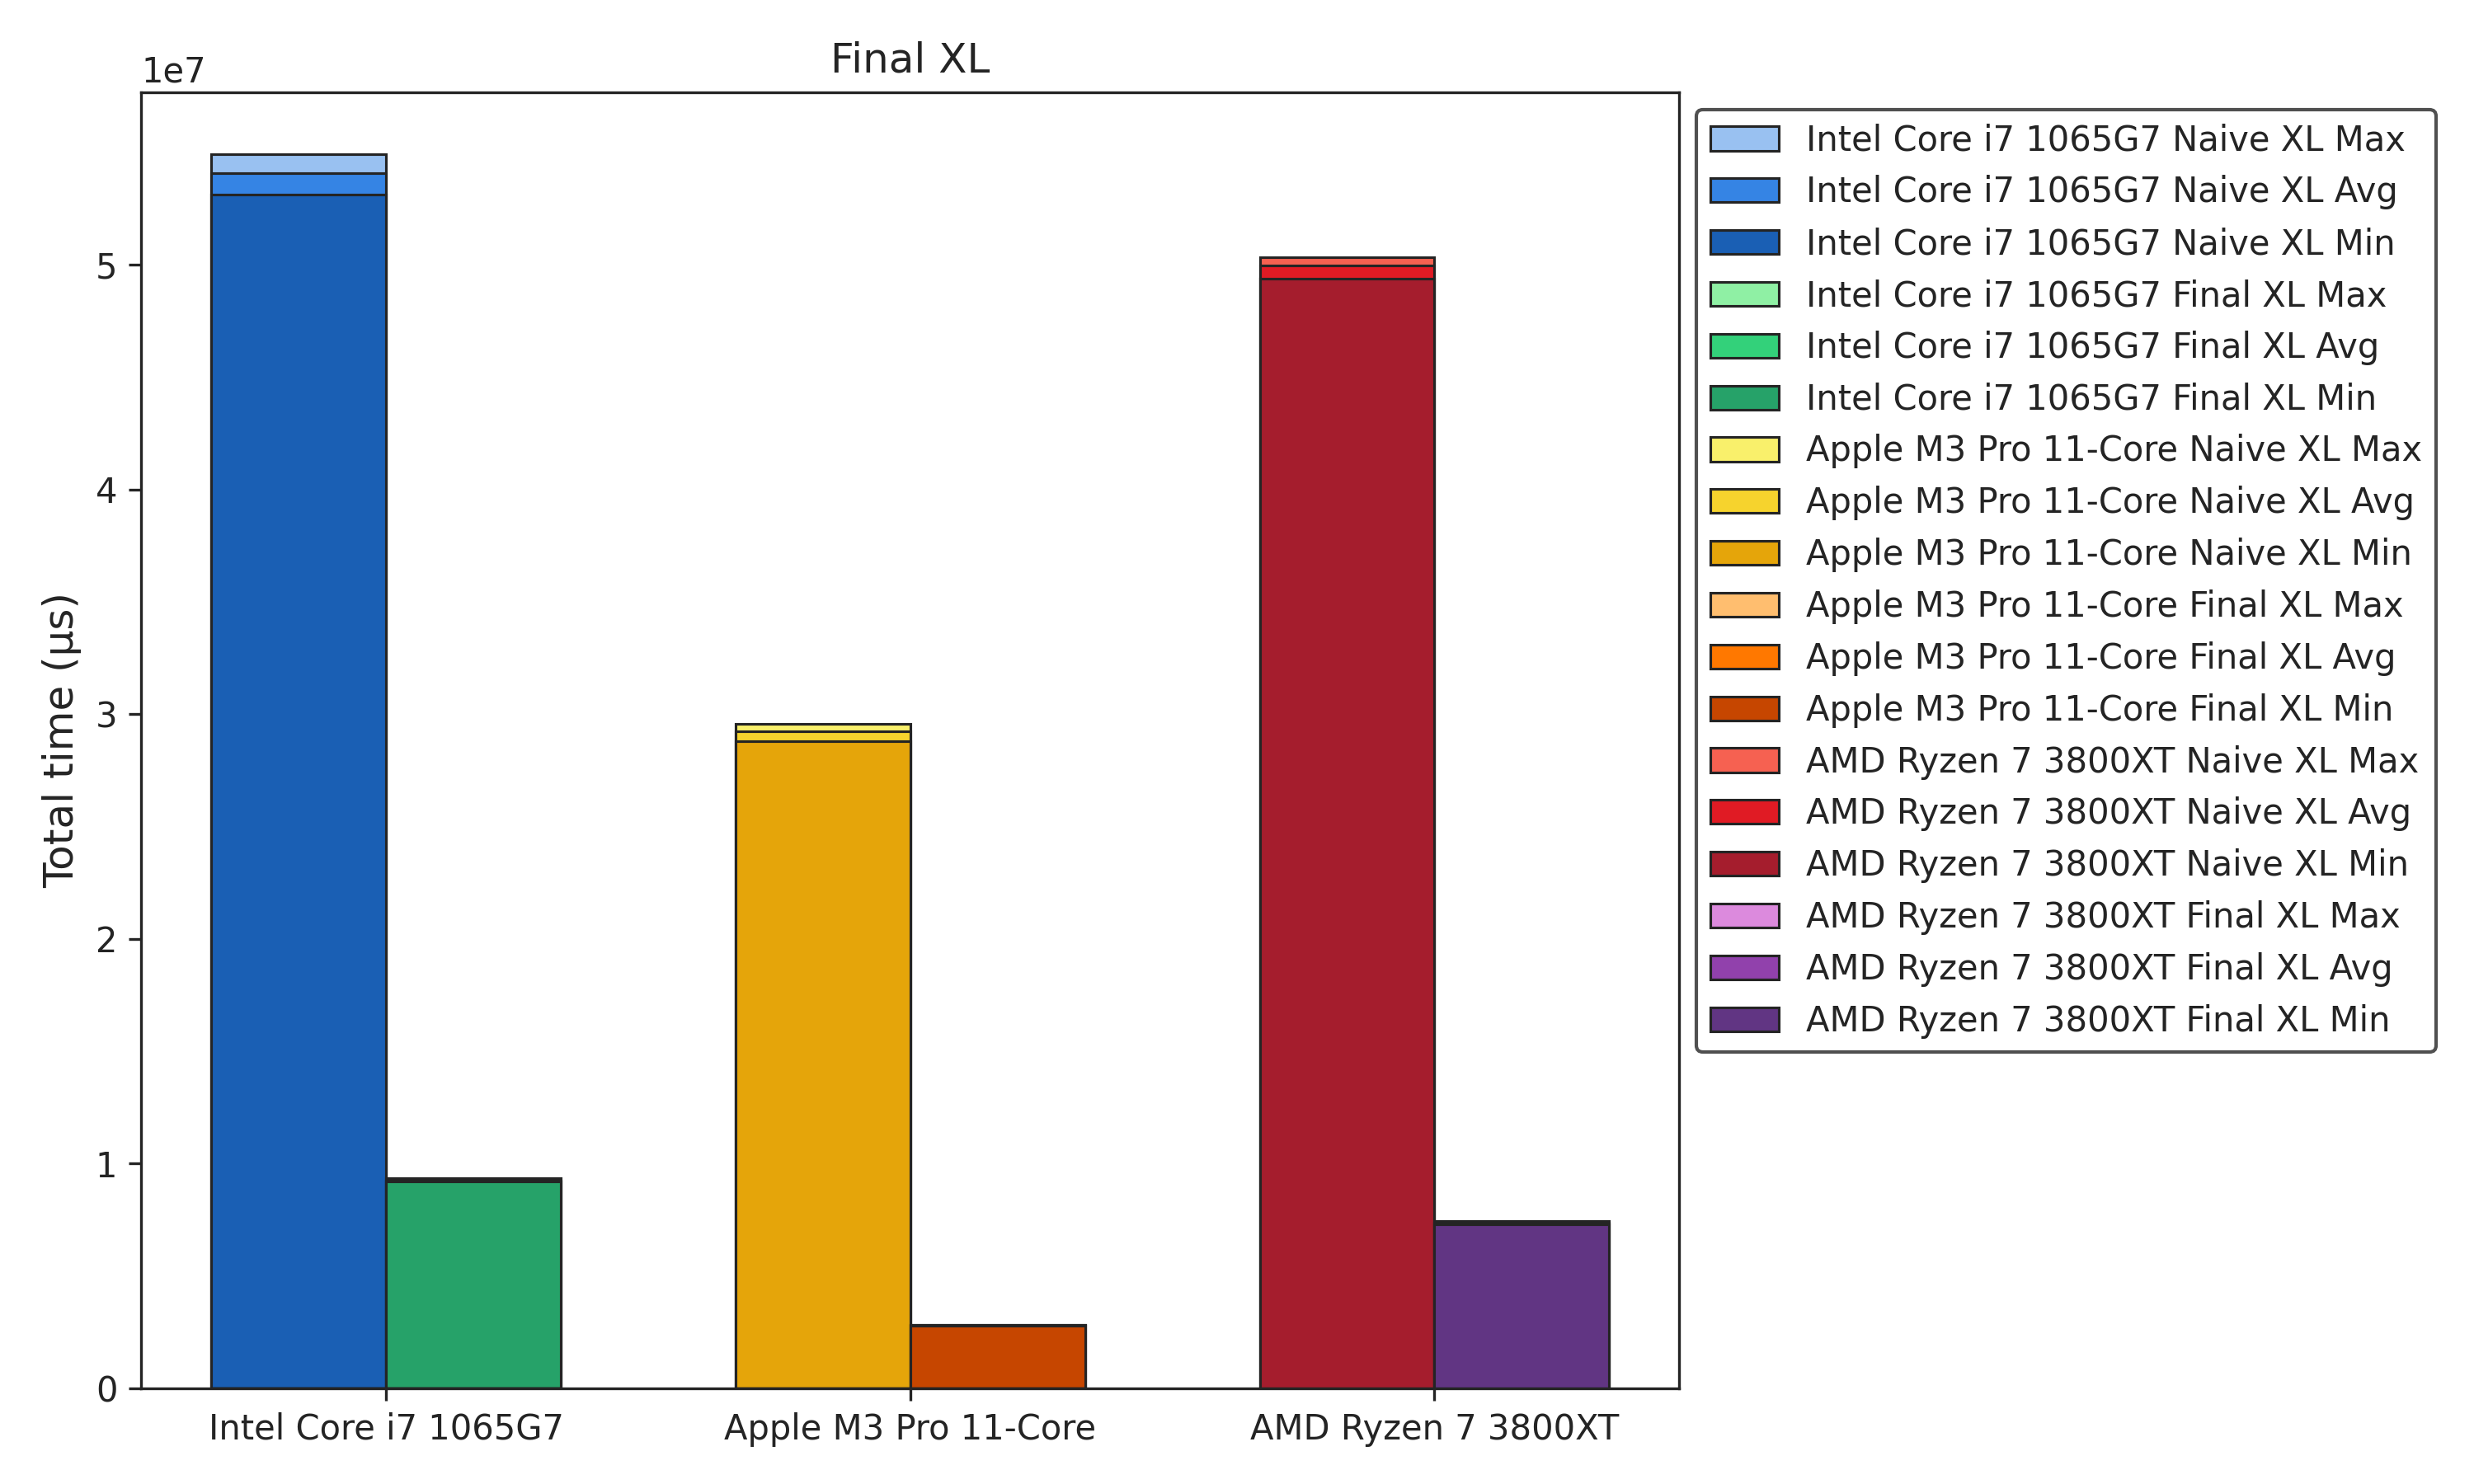
\includegraphics[width=\linewidth]{Graphs/Final XL.png}
  \caption{On the synthetic XL dataset}
 \label{fig:initial_vs_final_xl}
\end{subfigure}
\caption{Performance benchmarks comparing the initial and final implementation}
\label{fig:initial_vs_final}
\end{figure}
\begin{table}[htb!]
\centering
\caption{Inital vs. Final Implementation\label{tab:initial_vs_final}}
\begin{tabular}{p{5cm} p{2cm} p{2cm} p{2cm} p{2cm}}
\hline
Benchmark Name & Minimum Value ($\mu$s) & Average Value ($\mu$s) & Maximum Value ($\mu$s) & Standard Deviation \\
\hline
Intel Core i7-1065G7 \\
\hspace{0.5cm}Naive & 41783.0 & 43833.5 & 47517.0 & 1788.0 \\
\hspace{0.5cm}Final & 10725.0 & 11398.8 & 12087.0 & 417.5 \\
Apple M3 Pro 11-Core \\
\hspace{0.5cm}Naive & 26718.0 & 27648.4 & 28075.0 & 468.9 \\
\hspace{0.5cm}Final & 10575.0 & 11170.5 & 12407.0 & 618.4 \\
AMD Ryzen 7 3800XT \\
\hspace{0.5cm}Naive & 38841.0 & 39271.6 & 40180.0 & 379.2 \\
\hspace{0.5cm}Final & 21050.0 & 22202.5 & 23671.0 & 747.3 \\
\hline
Intel Core i7-1065G7 \\
\hspace{0.5cm}Naive XL & 53137471.0 & 54097305.1 & 54939589.0 & 549782.2 \\
\hspace{0.5cm}Final XL & 9195229.0 & 9246640.6 & 9369463.0 & 52836.7 \\
Apple M3 Pro 11-Core \\
\hspace{0.5cm}Naive XL & 28821610.0 & 29244264.5 & 29572155.0 & 226548.1 \\
\hspace{0.5cm}Final XL & 2783871.0 & 2802165.9 & 2824752.0 & 13541.5 \\
AMD Ryzen 7 3800XT \\
\hspace{0.5cm}Naive XL & 49407386.0 & 49970509.5 & 50337761.0 & 318289.1 \\
\hspace{0.5cm}Final XL & 7302691.0 & 7361732.2 & 7450227.0 & 50234.5 \\
\hline
\end{tabular}
\end{table}
\FloatBarrier

In this section, we combine all the optimizations from Chapter~\ref{sec:cpu-based-optimizations} that demonstrate a measurable improvement in performance. This includes, most notably, the optimized multithreading implementation with a parallelized image processing pipeline, which itself utilizes parallelized functions. Additionally, we integrate Arm Neon for Apple Silicon, AVX2 for the AMD processor, and AVX-512 for the Intel CPU. OpenMP and quantization, on the other hand, either show no improvement or lead to degraded performance and are therefore excluded.

For consistency and cross-platform comparability, we use the Clang compiler across all systems. As a result of these combined efforts, we observe at least a twofold increase in average performance. The effectiveness of these optimizations becomes even more pronounced as the problem size increases, clearly illustrating the value of investing time in thoughtful, well-structured optimization strategies rather than relying on naive and rapidly aging code.

In the context of modern large language models, such optimizations often mark the difference between an unfinished execution and acceptable runtime performance. However, not all optimizations meet expectations, so rigorous testing and evaluation remain essential.

It is also worth noting that many additional opportunities for improvement exist beyond those discussed here. In this paper, we focus on a representative subset, yet the potential for further gains remains significant — a promising indication of the value optimization can bring.
\section{GPU-Based Optimizations}\label{sec:gpu-based-optimizations}
\subsection{Overview of CUDA}

In the field of general-purpose GPU computing, two principal frameworks are predominantly utilized: Compute Unified Device Architecture (CUDA) and Open Computing Language (OpenCL).

CUDA, developed by NVIDIA, is a proprietary platform designed exclusively for the company's own graphics processing units. In contrast, OpenCL, maintained by the Khronos Group, is an open standard that supports a broad range of hardware architectures, including those from various GPU vendors, as well as CPUs and FPGAs.

CUDA is frequently regarded as more accessible due to its specialized scope and the cohesive integration with NVIDIA hardware, which enables highly optimized performance. Additionally, it is supported by a comprehensive suite of development tools and libraries, contributing to its widespread adoption within both academic and industrial contexts.

OpenCL, while offering broader hardware compatibility, is often associated with greater complexity and variable performance across different platforms. Furthermore, its tooling ecosystem is comparatively less mature and exhibits inconsistencies depending on the target device and vendor implementation.

Considering these differences, CUDA has emerged as the dominant framework for GPU-accelerated computation. Its deep integration within scientific computing and machine learning ecosystems, along with consistent performance and mature tooling, positions it as the preferred choice for high-performance applications. Consequently, CUDA will be employed in this project to implement the necessary GPU optimizations.
\subsection{CUDA Processing Flow}
\begin{figure}[htb!]
    \centering
    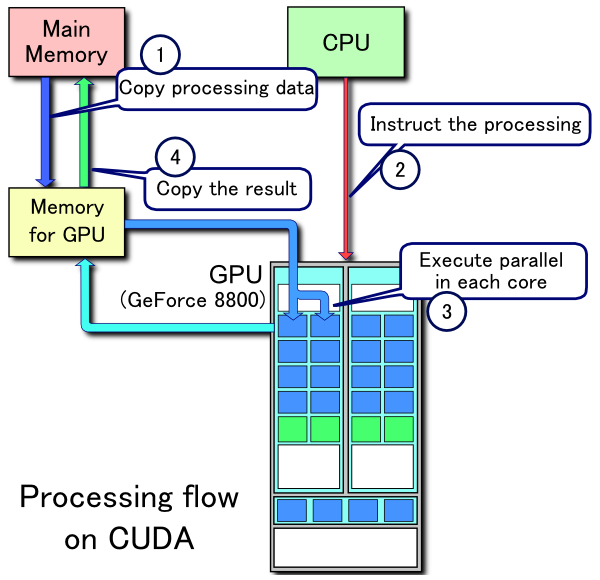
\includegraphics[width=0.6\linewidth]{CUDA/CUDA_processing_flow_(En).png}
    \caption{Example of CUDA processing flow\footnote{CUDA: \url{https://en.wikipedia.org/wiki/CUDA} (accessed April 10, 2025).}}
   \label{fig:cuda-processing-flow}
\end{figure}

Before leveraging the GPU for computation, it is essential to understand its basic execution model. The GPU does not operate independently and lacks control over program flow; instead, it is directed by the CPU. For efficient processing, the GPU uses its own high-speed memory, separate from the system’s main memory. Consequently, data required for computation must first be allocated in GPU memory and transferred from the host (CPU) memory. This memory transfer introduces significant latency and is often a primary bottleneck in GPU-based computing.

Once the necessary data is transferred, the CPU launches a CUDA kernel on the GPU, initiating parallel execution. This kernel is executed concurrently by a large number of lightweight GPU threads, enabling high throughput for data-parallel tasks.

After the GPU completes its computation, the resulting data must be copied back to main memory to be accessed or validated by the CPU. Similar to the initial transfer, this retrieval step also incurs overhead, which must be taken into account when optimizing GPU performance.
\subsection{CUDA Kernels}\label{subsec:cuda-kernels}
The initial implementation introduces considerable overhead. For instance, functions such as ReLU, which involve minimal computation, are inefficiently executed using separate CUDA kernels. While deploying a kernel for such trivial operations may seem unnecessary, it is implemented at this stage to maintain consistency and to support later improvements discussed in Section~\ref{subsec:eliminate-copy-overhead}.

As each function depicted in Figure~\ref{fig:graph} is executed independently on the GPU, data must be transferred between the host (CPU) and device (GPU) memory before and after each function call, significantly impacting performance. An example of this memory transfer process is shown in Listing~\ref{lst:cuda-memcpy}.

\begin{lstlisting}[
    caption={CUDA memory allocation and host-to-device copy},
    label={lst:cuda-memcpy},
    language=C++,
    numbers=left,
    numbersep=10pt,
    basicstyle=\fontsize{10}{10}\selectfont,
    breaklines=true,
    postbreak=\mbox{\textcolor{red}{$\hookrightarrow$}\space},
    frame=single,
]
// Calculate size of N x N matrix in bytes
size_t bytes_n = N * N * sizeof(float);
float* d_matrix;  // Device pointer
// Allocate memory on the GPU
cudaMalloc(&d_matrix, bytes_n);
// Copy matrix data from host (CPU) to device (GPU)
cudaMemcpy(d_matrix, a->m, bytes_n, cudaMemcpyHostToDevice);
\end{lstlisting}

Once the necessary data is in place, the CPU launches CUDA kernels to perform the required computations on the GPU. A CUDA kernel is a function executed in parallel by many threads, where each thread operates on a portion of the data. To determine its assigned workload, each thread accesses built-in variables such as \texttt{threadIdx} and \texttt{blockIdx}, which represent its position within a block and the block's position within a grid, respectively.

In CUDA's hierarchical execution model, threads are organized into blocks, and blocks are further arranged into a grid. This structure allows scalable parallelism across thousands of threads while supporting localized synchronization and memory sharing within thread blocks. Proper configuration of the block and grid dimensions is essential for efficient hardware utilization and performance. A representative example of a kernel configuration used for matrix multiplication is presented in Listing~\ref{lst:cuda-kernel-launch}. The corresponding kernel is shown in Listing~\ref{lst:cuda-kernel}.

\begin{lstlisting}[
    caption={Host-side CUDA kernel launch with block and grid configuration},
    label={lst:cuda-kernel-launch},
    language=C++,
    numbers=left,
    numbersep=10pt,
    basicstyle=\fontsize{10}{10}\selectfont,
    breaklines=true,
    postbreak=\mbox{\textcolor{red}{$\hookrightarrow$}\space},
    frame=single,
]
int THREADS = 16;
// Ensure full coverage in X (columns)
int BLOCKS_X = (N + THREADS - 1) / THREADS;
// Ensure full coverage in Y (rows)
int BLOCKS_Y = (M + THREADS - 1) / THREADS;  
// Define number of threads per block
dim3 threads(THREADS, THREADS);
// Define number of blocks needed in the grid
dim3 blocks(BLOCKS_X, BLOCKS_Y);
matmul_kernel<<<blocks, threads>>>(d_a, d_b, d_c, N, M, K);
\end{lstlisting}

\begin{lstlisting}[
    caption={CUDA matrix multiplication kernel},
    label={lst:cuda-kernel},
    language=C++,
    numbers=left,
    numbersep=10pt,
    basicstyle=\fontsize{10}{10}\selectfont,
    breaklines=true,
    postbreak=\mbox{\textcolor{red}{$\hookrightarrow$}\space},
    frame=single,
]
__global__ void matmul_kernel(const float* a, const float* b, 
    float* c, int N, int M, int K) {
    // Calculate the row and column index of the element
    int row = blockIdx.y * blockDim.y + threadIdx.y;
    int col = blockIdx.x * blockDim.x + threadIdx.x;
    // Boundary check to avoid accessing out-of-bounds memory
    if(row < M && col < N) {
        // Accumulator for the dot product
        float cValue = 0.0;  
        // Perform the dot product of
        // the row of A and the column of B
        for(int k = 0; k < K; k++) {
            cValue += a[row * K + k] * b[k * N + col];
        }
        // Write the computed value to the output matrix C
        c[row * N + col] = cValue;
    }
}
\end{lstlisting}
\subsection{Initial Benchmarks}
\begin{figure}[htb!]
\centering
\begin{subfigure}{.5\textwidth}
  \centering
  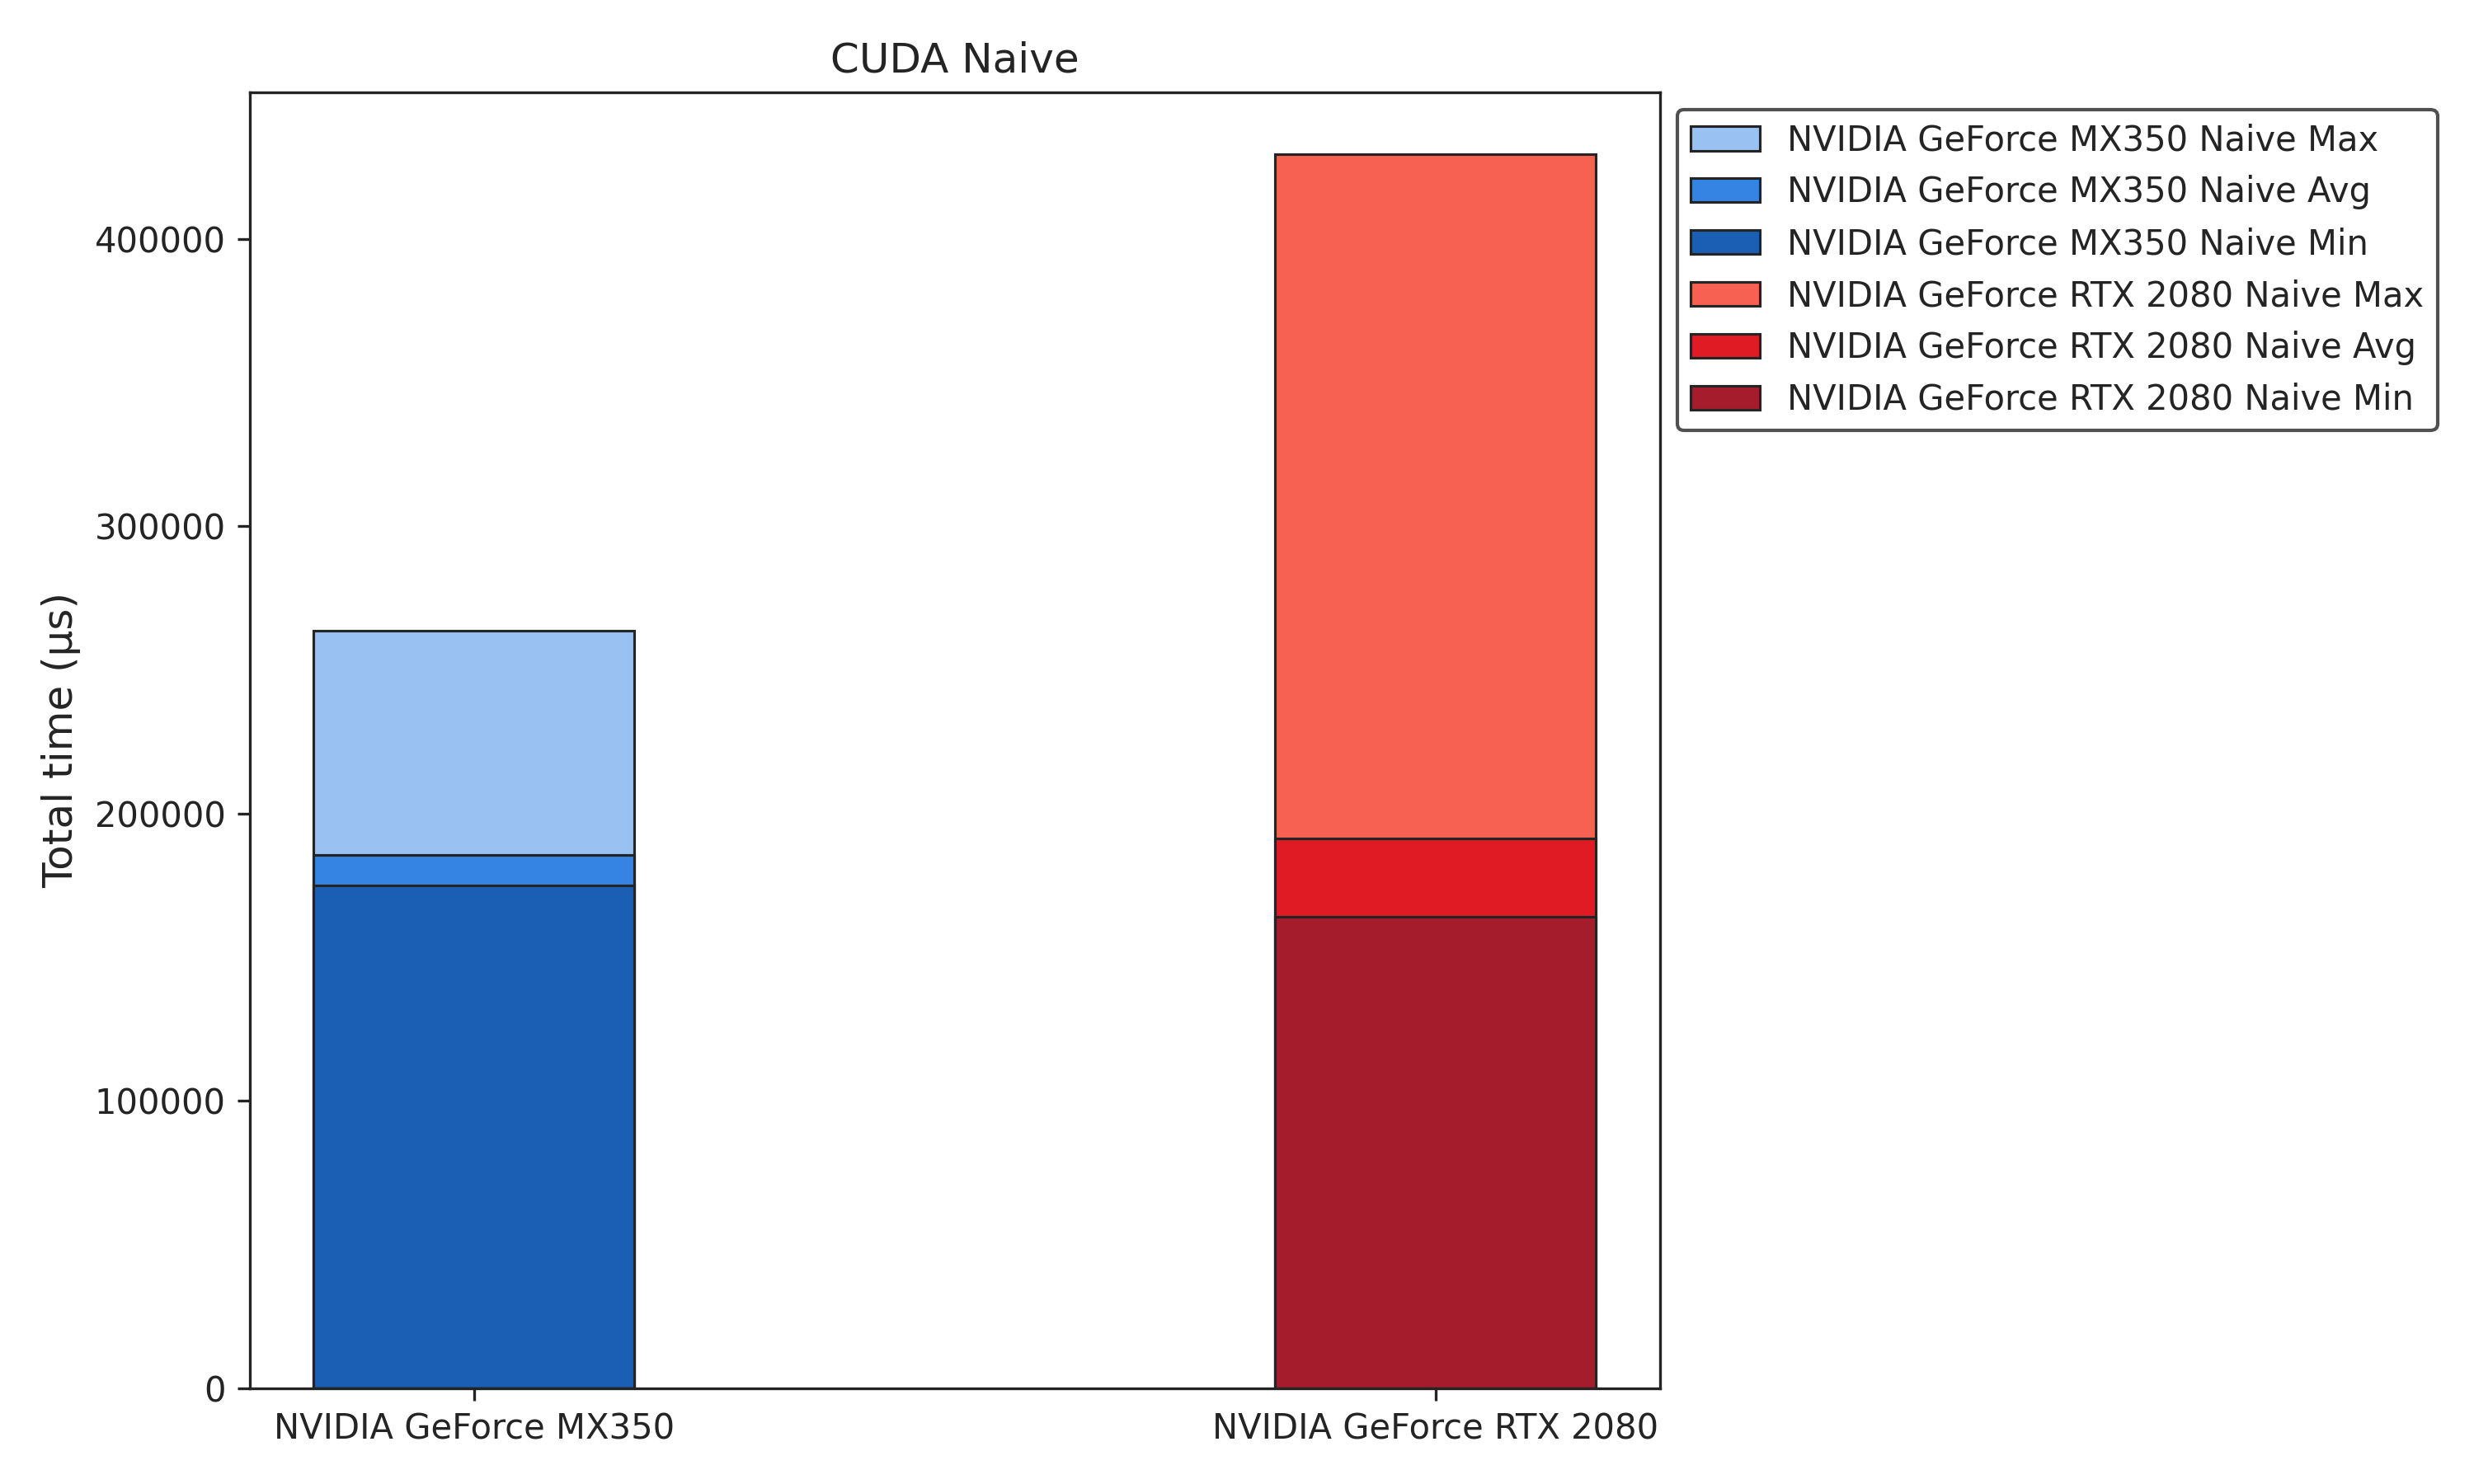
\includegraphics[width=\linewidth]{Graphs/CUDA.png}
  \caption{On the MNIST dataset}
\end{subfigure}%
\begin{subfigure}{.5\textwidth}
  \centering
  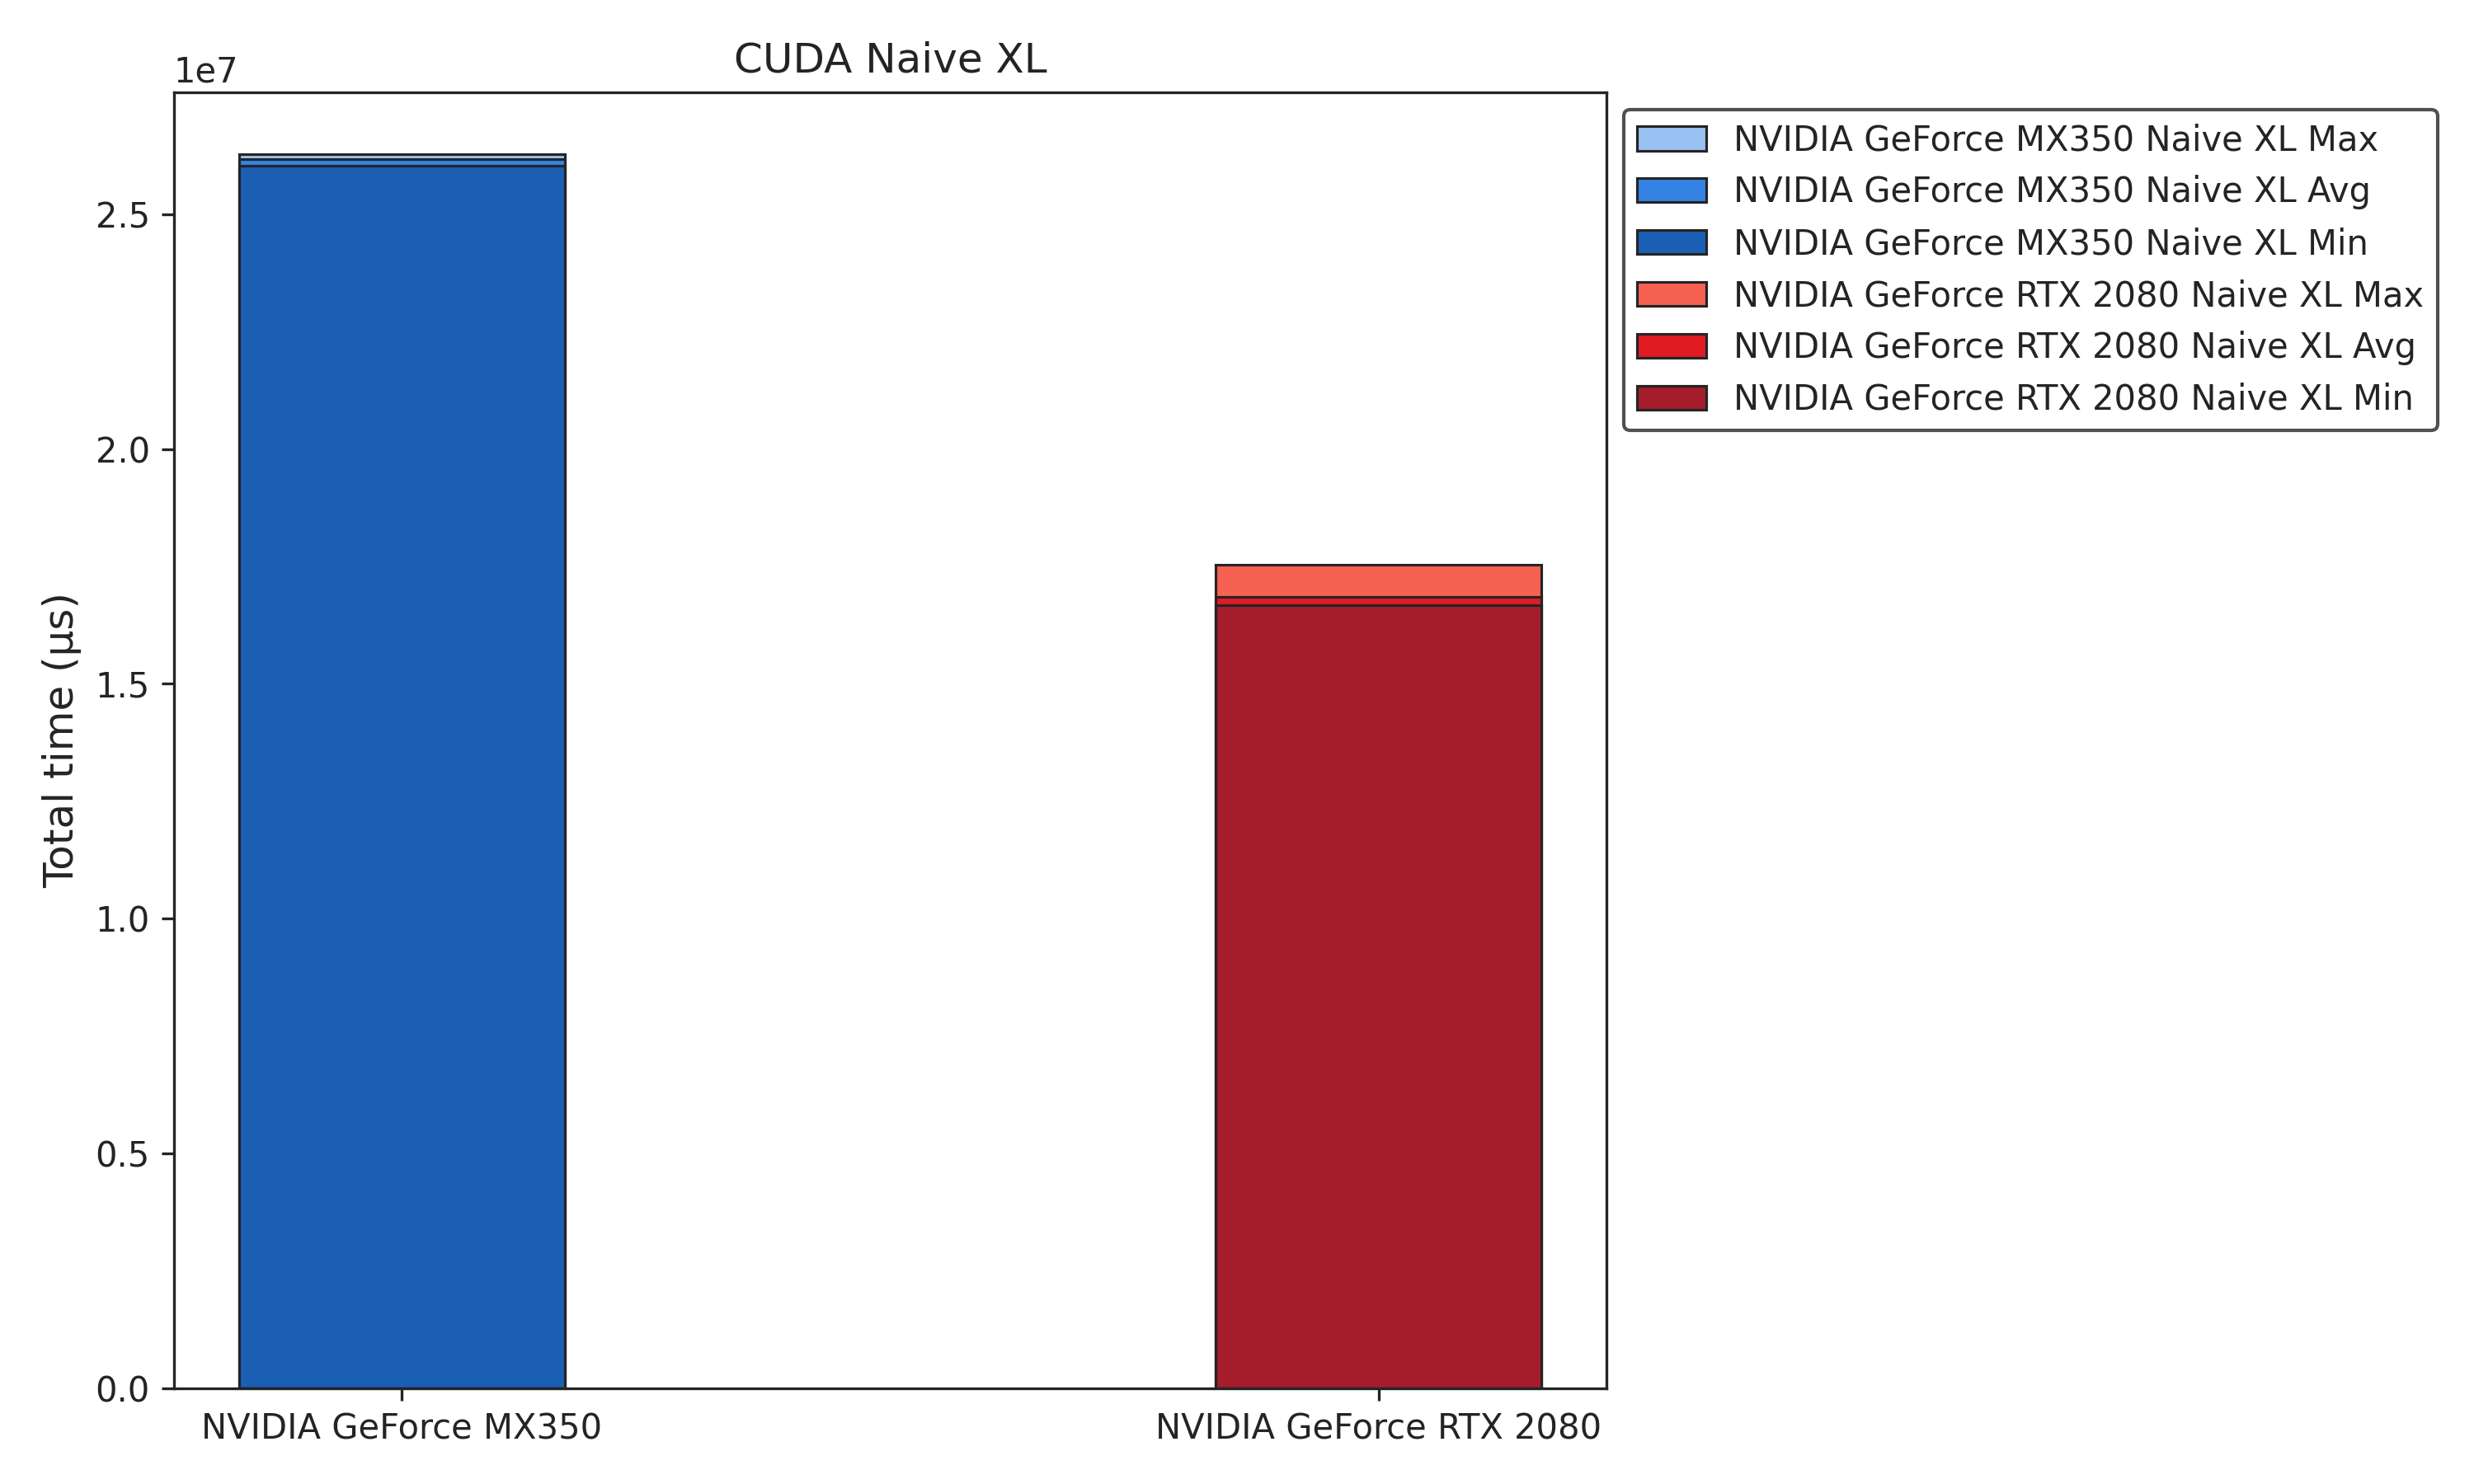
\includegraphics[width=\linewidth]{Graphs/CUDA XL.png}
  \caption{On the synthetic XL dataset}
\end{subfigure}
\caption{Performance benchmarks of the initial CUDA implementation}
\label{fig:cuda-initial}
\end{figure}

\begin{table}[htb!]
\centering
\caption{Initial CUDA Implementation\label{tab:initial_cuda}}
\begin{tabular}{p{5cm} p{2cm} p{2cm} p{2cm} p{2cm}}
\hline
Naive CUDA Implementation & Minimum Value ($\mu$s) & Average Value ($\mu$s) & Maximum Value ($\mu$s) & Standard Deviation \\
\hline
NVIDIA GeForce MX350 \\
\hspace{0.5cm}Naive & 174935.0 & 185643.7 & 263690.0 & 26088.6 \\
NVIDIA GeForce RTX 2080 \\
\hspace{0.5cm}Naive & 163977.0 & 191287.6 & 429508.0 & 79409.7 \\
\hline
NVIDIA GeForce MX350 \\
\hspace{0.5cm}Naive XL & 26024991.0 & 26167448.5 & 26279652.0 & 87379.6 \\
NVIDIA GeForce RTX 2080 \\
\hspace{0.5cm}Naive XL & 16678725.0 & 16850845.9 & 17539716.0 & 242817.9 \\
\hline
\end{tabular}
\end{table}
\FloatBarrier

The benchmark results for the initial implementation are presented in Figure~\ref{fig:cuda-initial}, with corresponding numerical values listed in Table~\ref{tab:initial_cuda}. On the MNIST dataset, the RTX 2080 exhibited a slight average performance decrease of 3.0\% compared to the MX350. In contrast, for the synthetic XL dataset, the RTX 2080 achieved an average performance improvement of 35.6\% relative to the MX350.

This initial evaluation serves as a baseline for assessing GPU utilization in the context of this project. The benchmarks were executed on the two mentioned NVIDIA GPUs. Detailed hardware specifications for both systems are provided in Table~\ref{tab:gpu}.

As discussed in Section~\ref{subsec:cuda-kernels}, the results reflect a preliminary implementation that lacks optimization. This version incurs substantial overhead primarily due to redundant memory transfers between host and device. Moreover, all data is stored in global memory, without the use of lower-latency alternatives such as shared or constant memory. The configuration of CUDA threads was also not optimized for hardware capabilities, but rather selected to ensure functional correctness.

Despite the hardware disparity, the MX350 produced competitive results on the MNIST dataset. However, this outcome is largely influenced by the small problem size, which diminishes the impact of the RTX 2080’s greater computational resources. The performance differences observed align with the architectural distinctions outlined in Table~\ref{tab:gpu}.

An important observation is the unusually high maximum runtime recorded for the MNIST dataset. This anomaly is attributed to CUDA runtime initialization, which introduces a fixed overhead prior to kernel execution. While necessary, this overhead becomes disproportionately significant for small workloads, where it may exceed the kernel's execution time. This illustrates a fundamental limitation of GPU acceleration for low-complexity tasks.

In the following sections, a series of targeted optimizations will be applied to improve computational efficiency and better exploit the capabilities of the underlying GPU hardware.
\subsection{Thread Utilization and Early Memory Transfer Improvements}\label{subsec:cuda-first-improvements}
The initial optimization phase focused on improving thread-level parallelism and reducing redundant memory transfers. First, the number of threads per block was increased to the architectural maximum supported by the hardware, which, for both tested GPUs, is 1024 threads per block. This change aims to enhance occupancy and better utilize the available parallelism of modern GPU architectures.

In parallel, the first step toward reducing memory transfer overhead was implemented. Specifically, the copying of the input and output matrices was moved outside the computation loop. This modification eliminates unnecessary and repeated data transfers between host and device memory, thereby improving efficiency.

These optimizations are expected to yield a measurable improvement in execution time. The resulting performance metrics are presented in Section~\ref{subsec:cuda-int-res-1}.
\subsection{Intermidiate Benchmarks}\label{subsec:cuda-int-res-1}
\begin{figure}[htb!]
\centering
\begin{subfigure}{.5\textwidth}
  \centering
  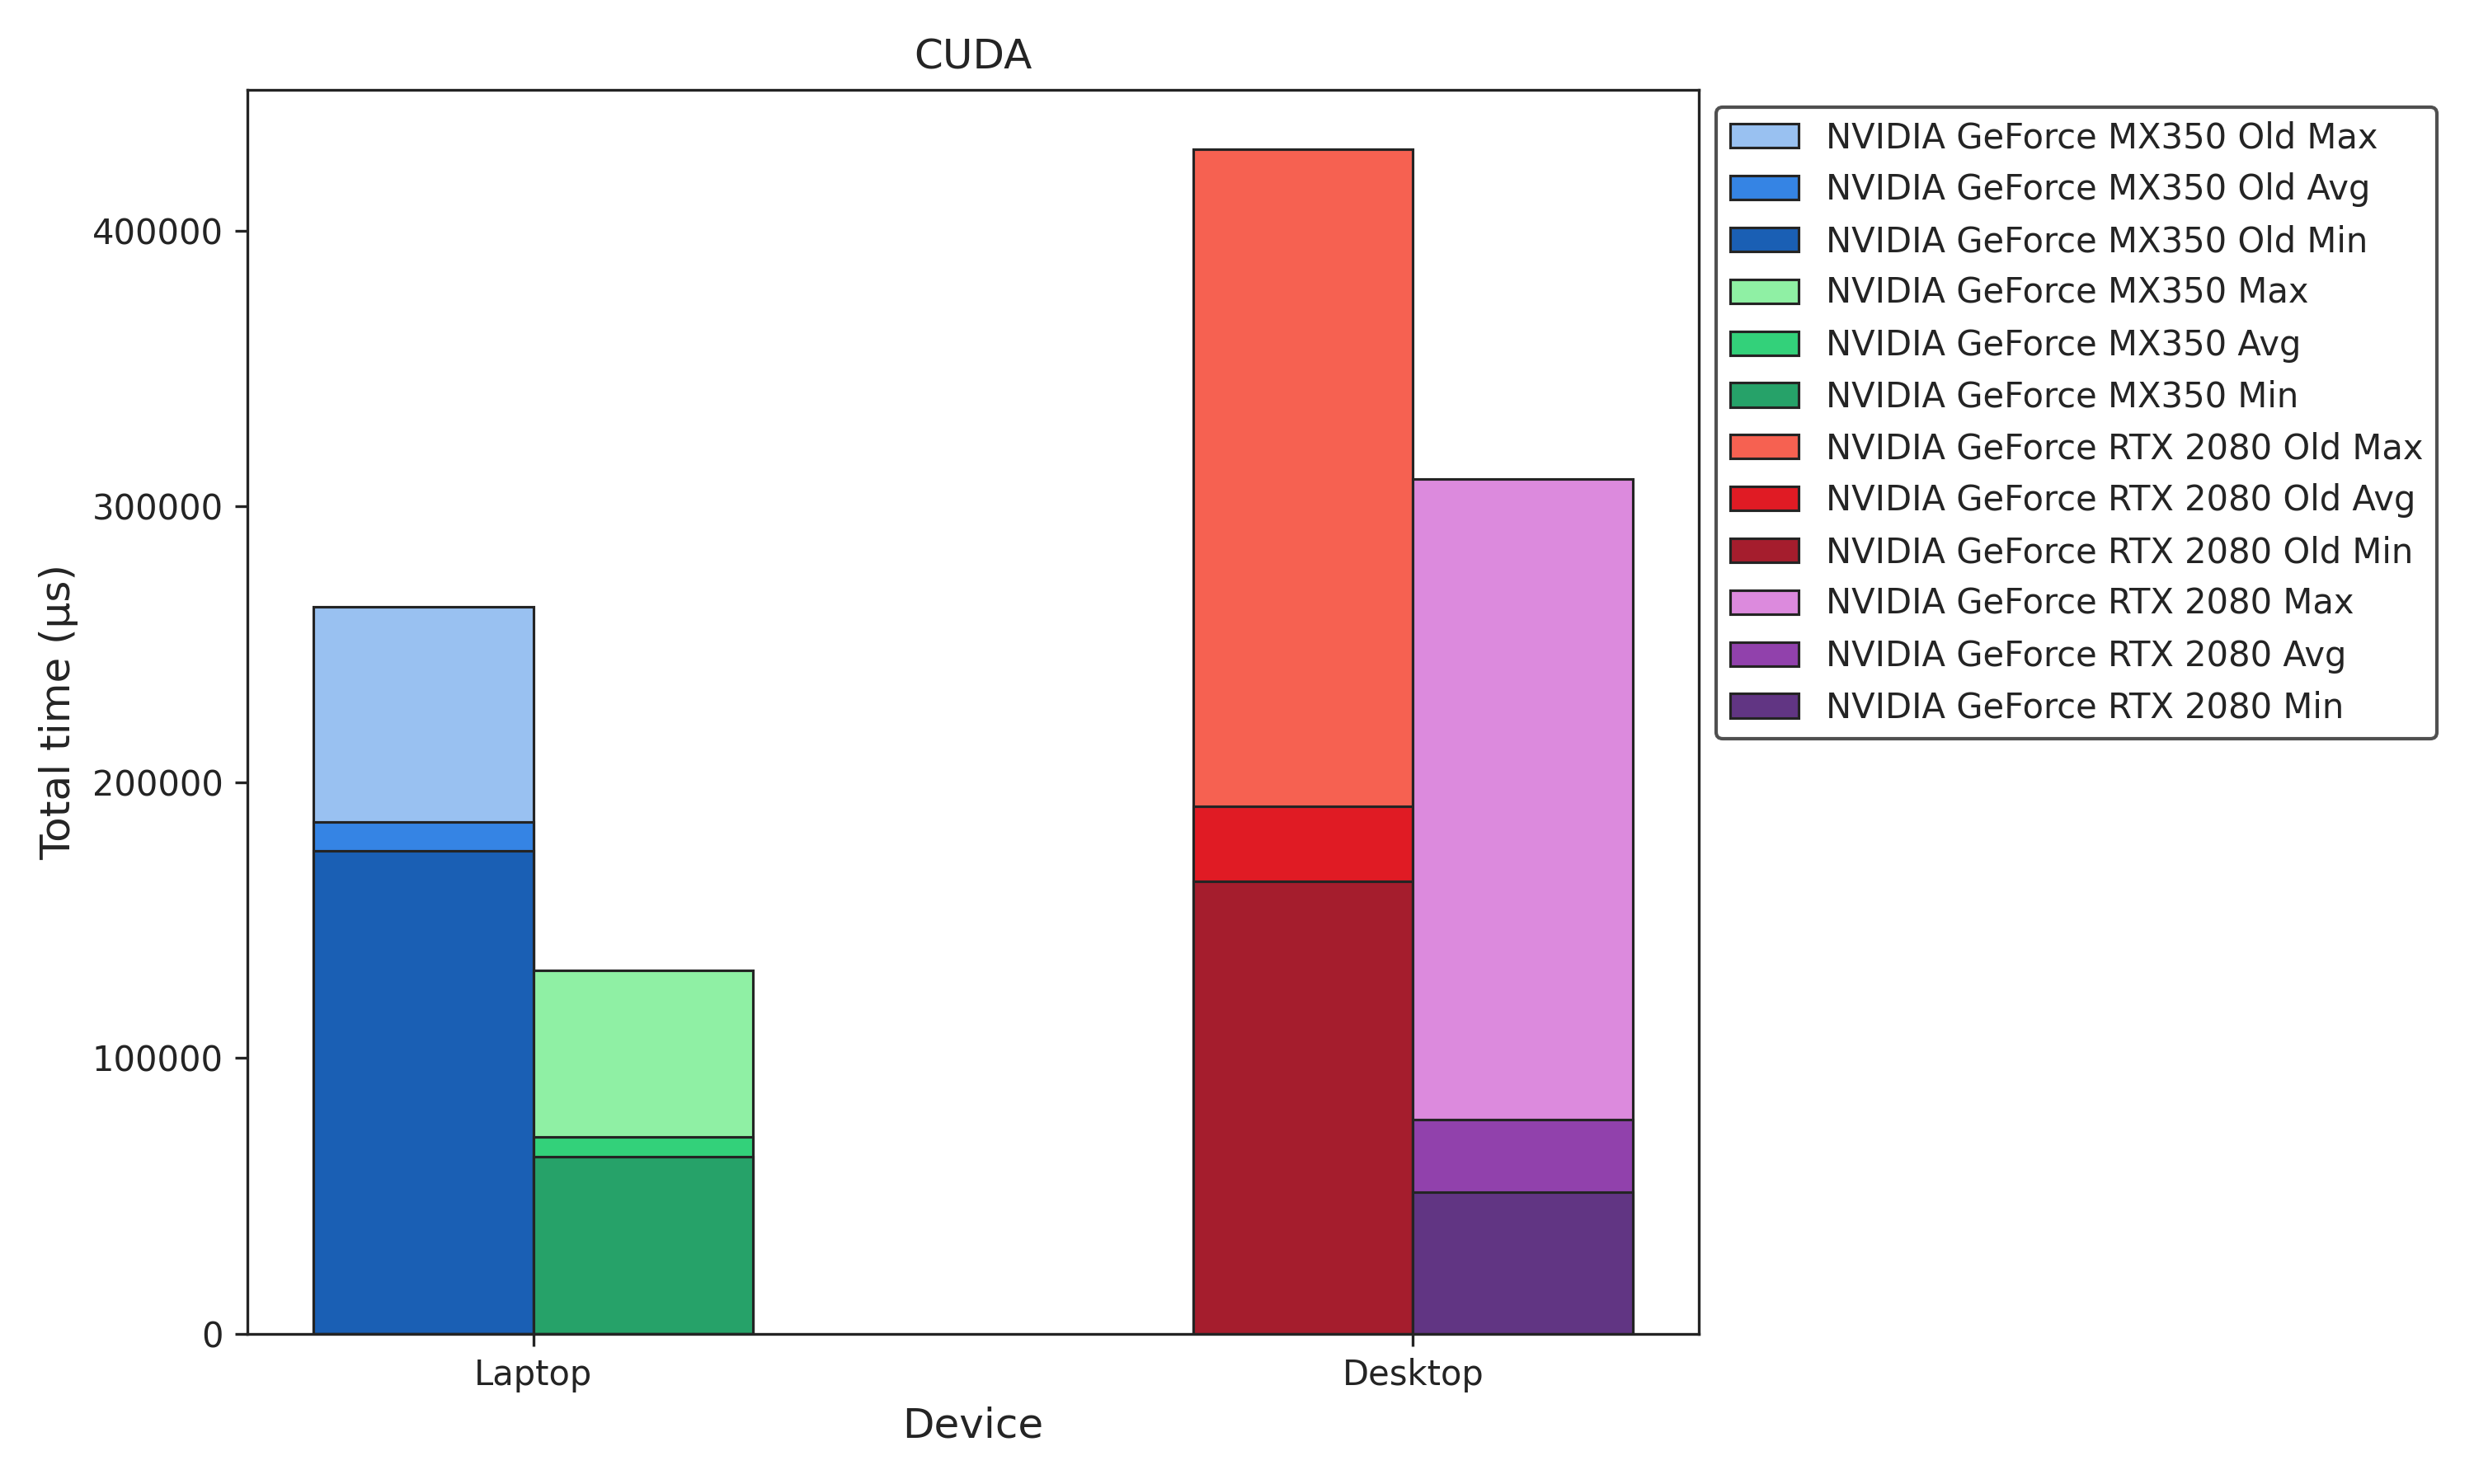
\includegraphics[width=\linewidth]{CUDA/CUDA_thread_optimization.png}
  \caption{On the MNIST dataset}
\end{subfigure}%
\begin{subfigure}{.5\textwidth}
  \centering
  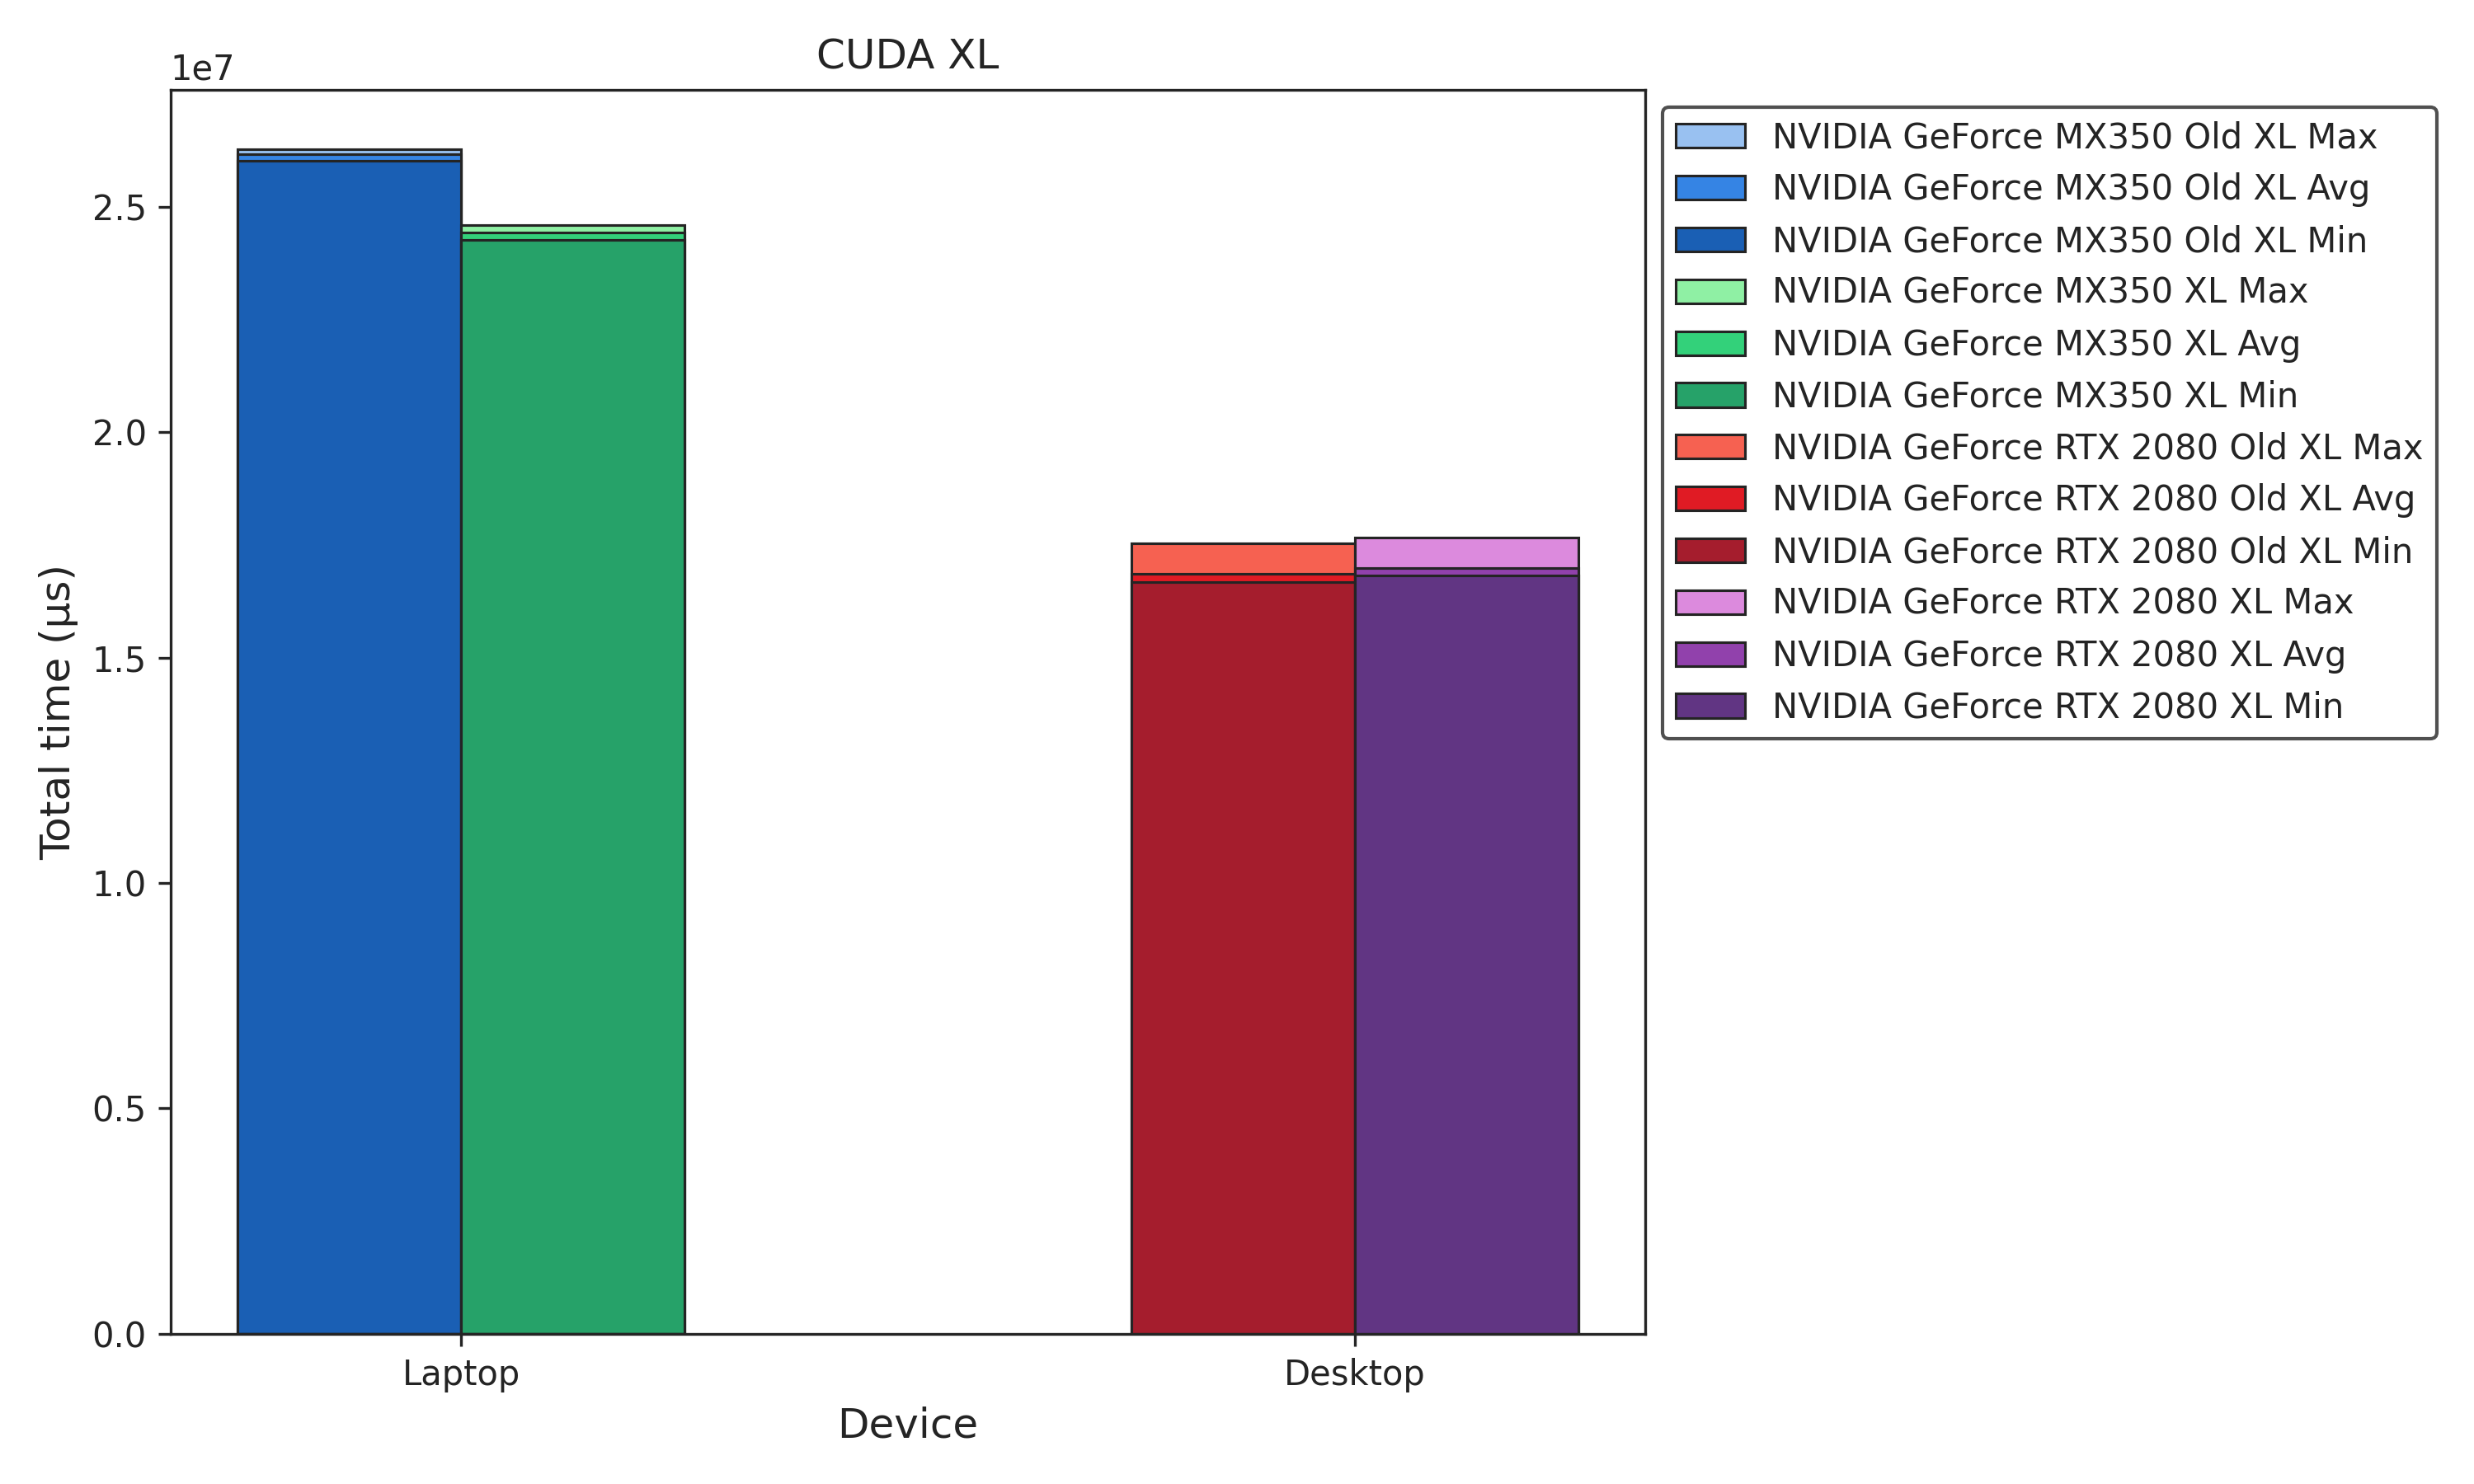
\includegraphics[width=\linewidth]{CUDA/CUDA XL_thread_optimization.png}
  \caption{On the synthetic XL dataset}
\end{subfigure}
\caption{Performance benchmarks of the CUDA implementation with optimized thread-level parallelism and first memory transfer overhead reductions}
\label{fig:cuda-intermediate-1}
\end{figure}

\begin{table}[htb!]
\centering
\caption{CUDA Implementation\label{tab:cuda-intermediate-1}}
\begin{tabular}{p{5.5cm} p{2cm} p{2cm} p{2cm} p{2cm}}
\hline
Benchmark Name & Minimum Value ($\mu$s) & Average Value ($\mu$s) & Maximum Value ($\mu$s) & Standard Deviation \\
\hline
NVIDIA GeForce MX350 \\
\hspace{0.5cm}Old & 174935.0 & 185643.7 & 263690.0 & 26088.6 \\
\hspace{0.5cm}New & 64061.0 & 71365.2 & 131868.0 & 20169.5 \\
NVIDIA GeForce RTX 2080 \\
\hspace{0.5cm}Old & 163977.0 & 191287.6 & 429508.0 & 79409.7 \\
\hspace{0.5cm}New & 51334.0 & 77513.5 & 309910.0 & 77468.6 \\
\hline
NVIDIA GeForce MX350 \\
\hspace{0.5cm}Old XL & 26024991.0 & 26167448.5 & 26279652.0 & 87379.6 \\
\hspace{0.5cm}New XL & 24271828.0 & 24437752.1 & 24595043.0 & 102639.1 \\
NVIDIA GeForce RTX 2080 \\
\hspace{0.5cm}Old XL & 16678725.0 & 16850845.9 & 17539716.0 & 242817.9 \\
\hspace{0.5cm}New XL & 16812469.0 & 16979213.1 & 17664752.0 & 242977.9 \\
\hline
\end{tabular}
\end{table}
\FloatBarrier

The performance results after the initial optimization phase are presented in Figure~\ref{fig:cuda-intermediate-1}, with detailed values listed in Table~\ref{tab:cuda-intermediate-1}. On the MNIST dataset, the average performance across both GPUs improved by 60.5\%, with the NVIDIA GeForce MX350 showing a 61.6\% increase and the RTX 2080 achieving a 59.5\% improvement. On the synthetic XL dataset, the average performance gain was more modest at 3.7\%. The MX350 showed a 6.6\% increase, whereas the RTX 2080 experienced a slight decline of 0.8\%.

These results follow the optimizations outlined in Section~\ref{subsec:cuda-first-improvements} and demonstrate a significant increase in computational efficiency, particularly for the MNIST workload. The execution time was reduced drastically, despite the fact that CUDA runtime initialization—still included in these measurements—remains a non-negligible overhead. This constant initialization cost highlights the relative impact of the optimizations, independent of setup time. In subsequent benchmarks, this overhead will be excluded to better isolate improvements in kernel execution.

For the synthetic XL dataset, performance gains were limited and observed only on the laptop GPU. This is likely due to the MX350’s relatively slower memory subsystem, where reduced memory transfer overhead provides a more pronounced benefit. In contrast, the RTX 2080 showed no significant improvement, which can be attributed to the insufficient size of the dataset relative to the GPU’s capabilities—resulting in underutilization of its parallel resources.

In the next optimization stages, the focus will shift toward enhancing performance on larger workloads, particularly for high-end hardware. This includes further reduction of memory transfer bottlenecks and increased parallelism to better exploit the architectural potential of the RTX 2080.
\subsection{Copy Overhead Elimination}\label{subsec:eliminate-copy-overhead}
Building upon the initial efforts to reduce memory transfer overheads in Section~\ref{subsec:cuda-first-improvements}, this stage focuses on fully eliminating unnecessary data movement during computation. The goal is to establish a memory-efficient execution pipeline by transferring all required data to the GPU before the computation begins, performing the entire workload on the device, and copying the final results back to the host memory only after all computations have completed.

This approach avoids intermediate memory transfers between the host and device, which previously occurred after each individual operation within the neural network. Instead, intermediate results are retained in device memory and directly passed between successive CUDA kernels. By maintaining all data on the GPU throughout the computation, we effectively implement a GPU memory pipeline that minimizes latency and maximizes throughput.

If the assumptions regarding memory transfer overheads are correct, this optimization is expected to yield a substantial performance improvement. The reduction of host-device communication to a single transfer at the beginning and end of execution should eliminate one of the most significant performance bottlenecks observed in earlier stages.
\subsection{Constant Memory Optimization}\label{subsec:cuda-constant-memory}
Constant memory is a small, read-only memory region located on the GPU, specifically optimized for scenarios in which all threads access the same data values. With a limited capacity of 64~KB, it is best suited for small datasets that remain unchanged throughout the computation. One of its primary advantages lies in its on-chip caching mechanism, which enables broadcast access across all threads within a warp, thereby significantly reducing memory access latency compared to global memory.

A key limitation of constant memory is its reduced flexibility, as array sizes must typically be fixed at compile time.

In the context of this project, constant memory proves particularly beneficial for implementing two-dimensional convolutions. The convolution kernels used in the benchmarks are of fixed size (3$\times$3), initialized once at the beginning of the computation, and remain constant throughout execution. These properties make them ideal candidates for placement in constant memory.

By storing the convolution kernel in constant memory, all threads involved in the computation can access the shared values efficiently, thereby reducing redundant global memory accesses. This not only lowers overall memory latency but also improves bandwidth utilization. The optimization is particularly effective for convolution operations, where multiple threads repeatedly access the same kernel values, leading to improved computational throughput.
\subsection{Intermidiate Benchmarks}\label{subsec:cuda-int-res-2}
\begin{figure}[htb!]
\centering
\begin{subfigure}{.5\textwidth}
  \centering
  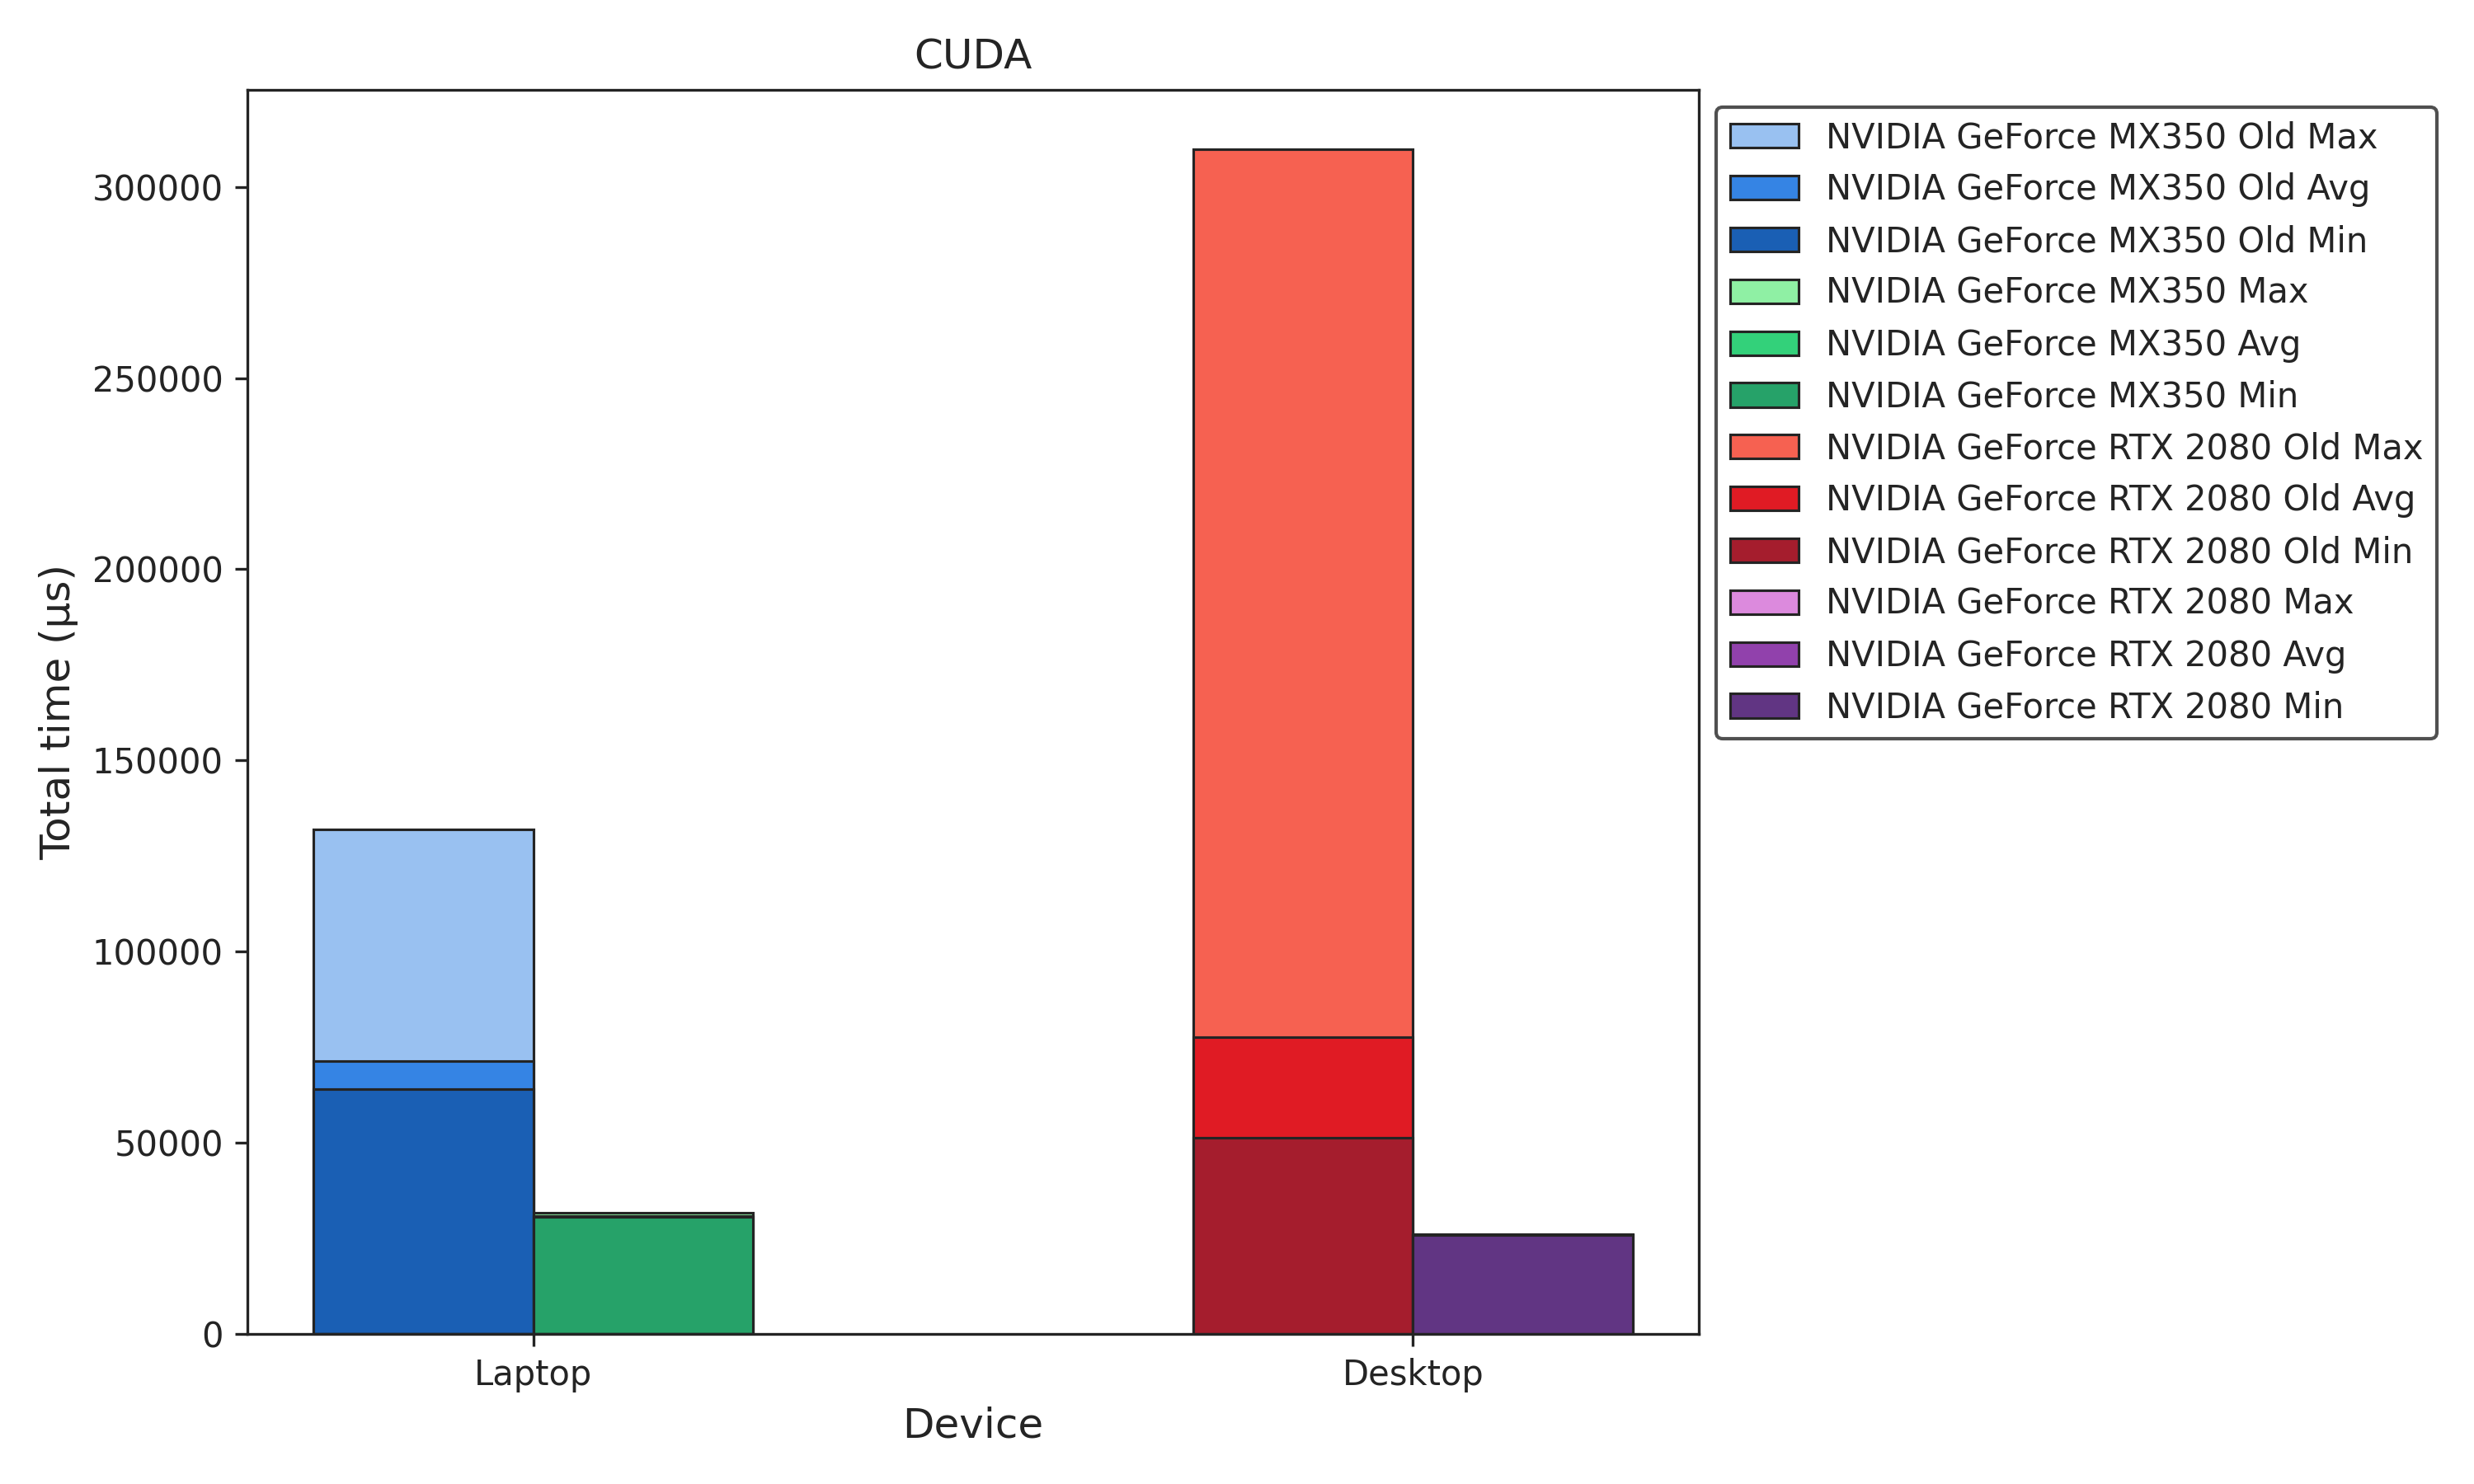
\includegraphics[width=\linewidth]{CUDA/CUDA_copy_overhead_eliminiation.png}
  \caption{On the MNIST dataset}
\end{subfigure}%
\begin{subfigure}{.5\textwidth}
  \centering
  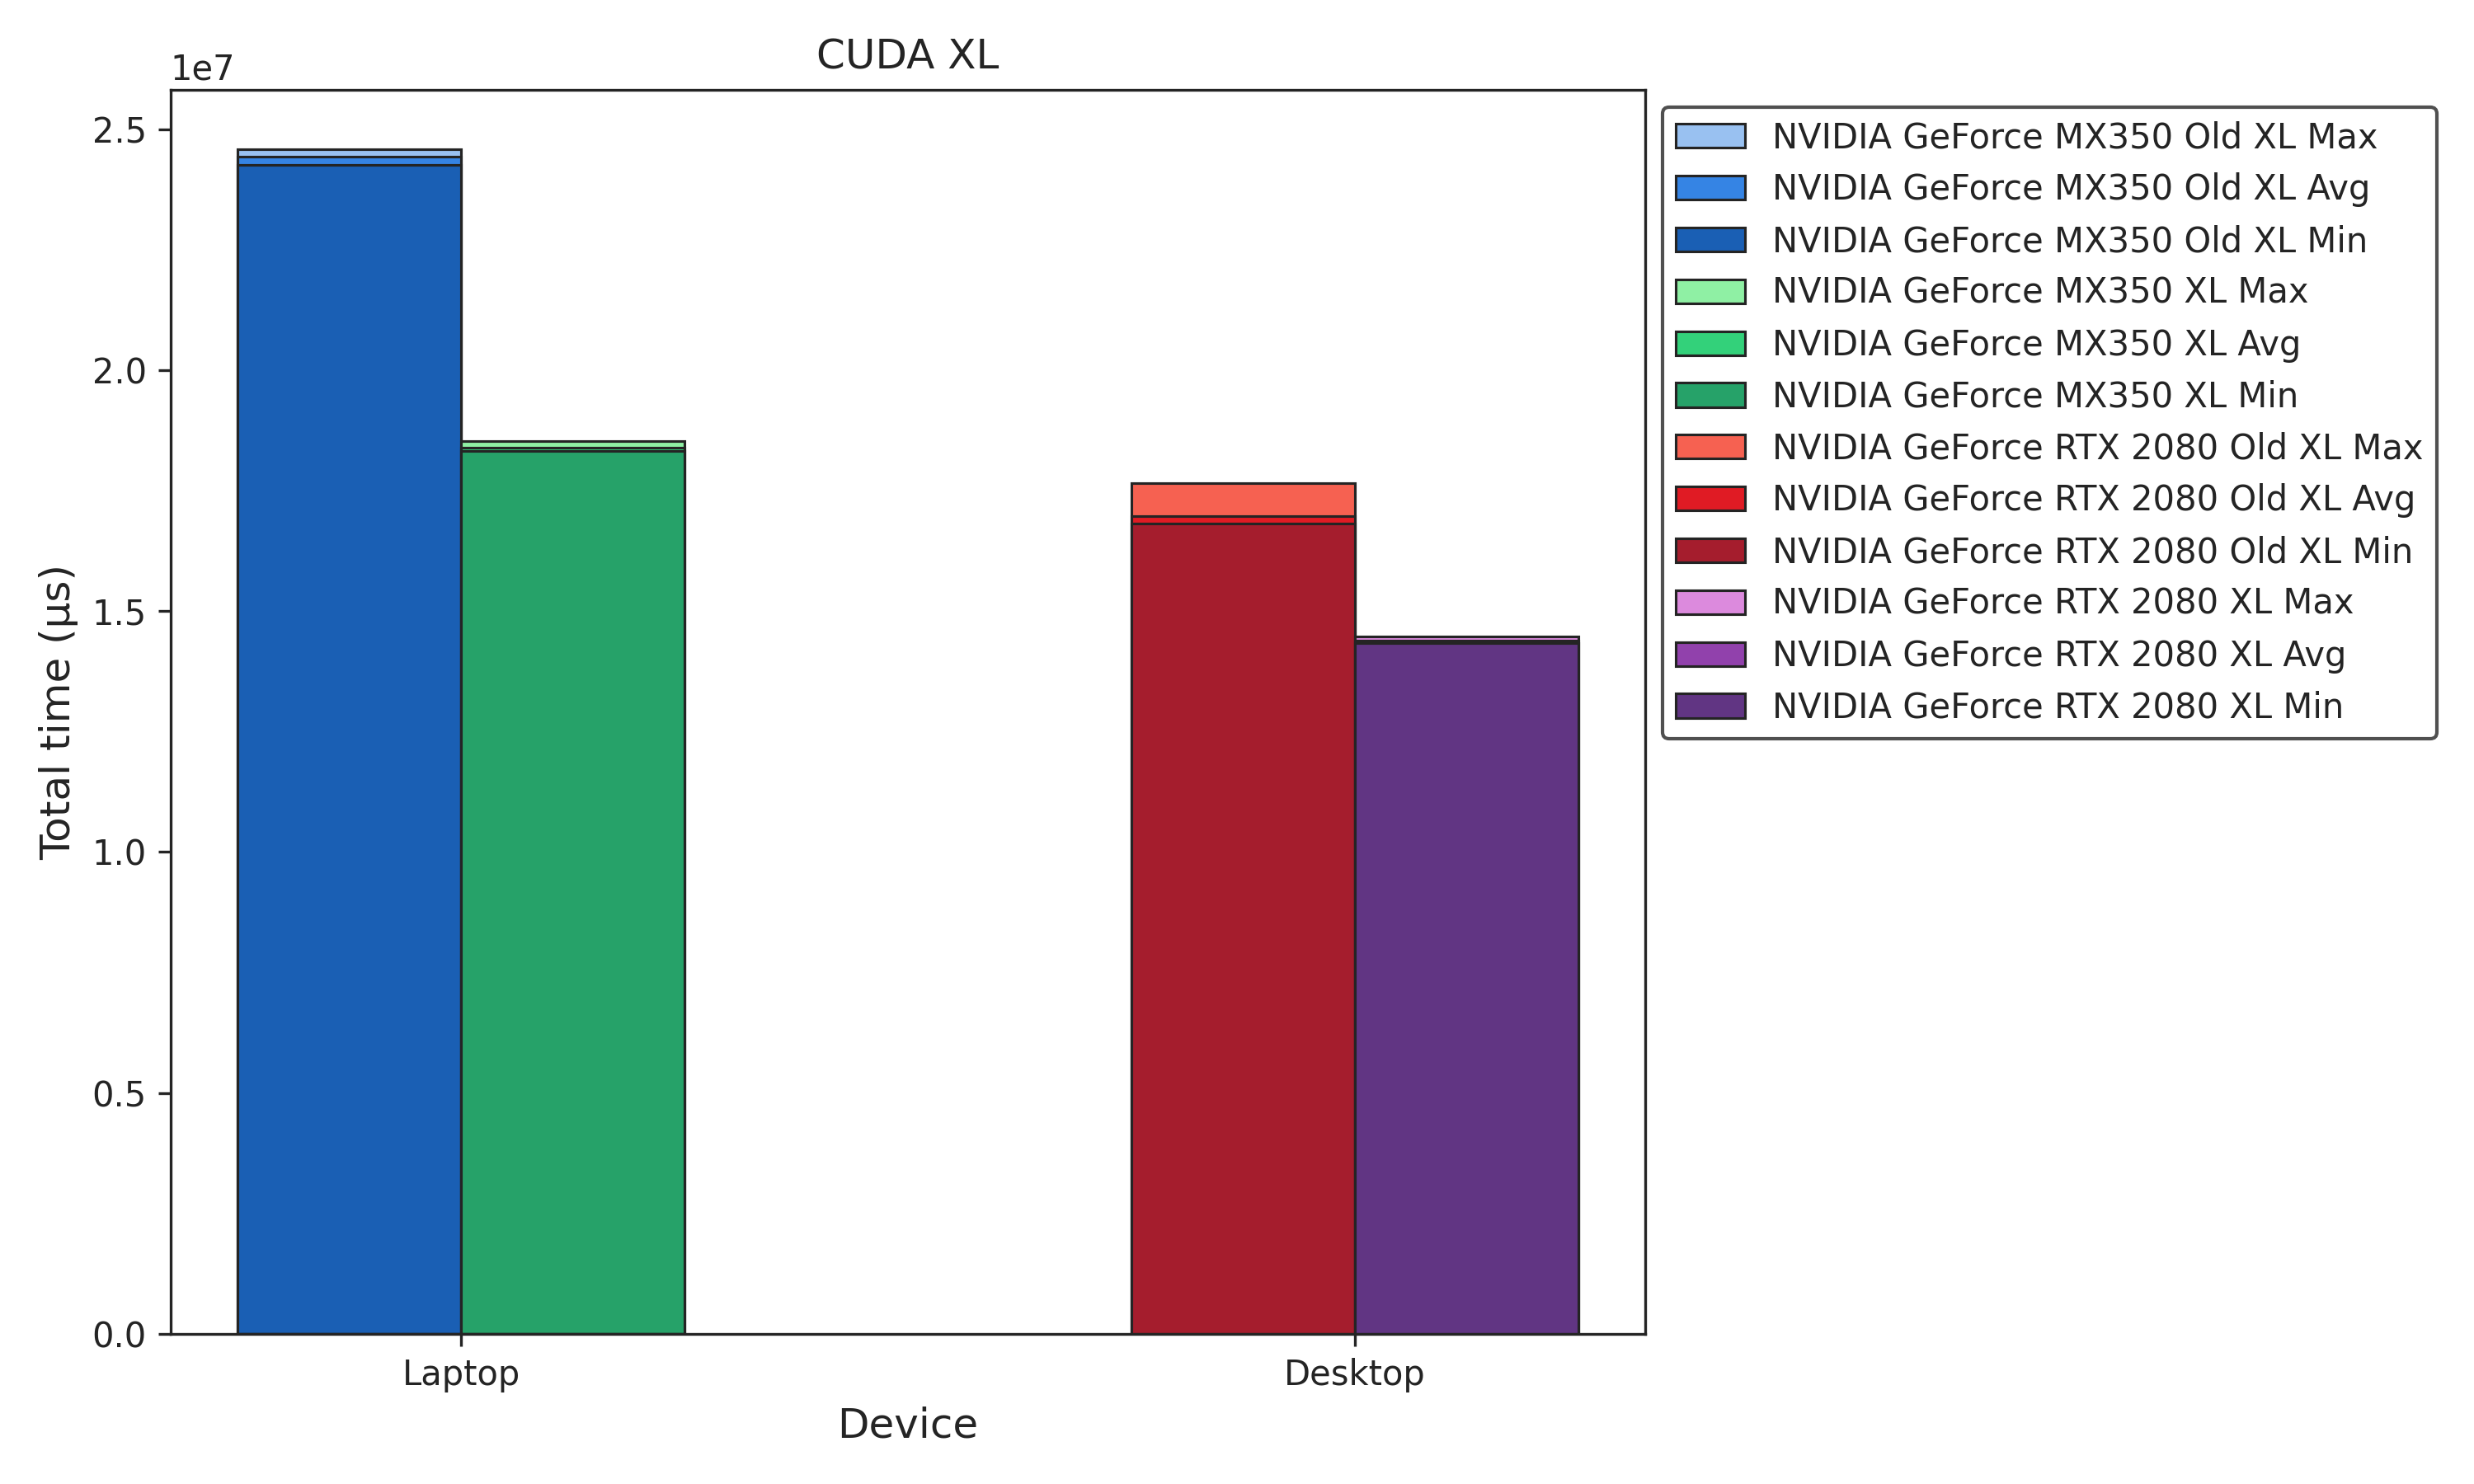
\includegraphics[width=\linewidth]{CUDA/CUDA XL_copy_overhead_elimination.png}
  \caption{On the synthetic XL dataset}
\end{subfigure}
\caption{Performance benchmarks of the CUDA implementation, extending previous optimizations with constant memory integration and removal of redundant copy operations}
\label{fig:cuda-intermediate-2}
\end{figure}

\begin{table}[htb!]
\centering
\caption{CUDA Implementation\label{tab:cuda-intermediate-2}}
\begin{tabular}{p{5.5cm} p{2cm} p{2cm} p{2cm} p{2cm}}
\hline
Benchmark Name & Minimum Value ($\mu$s) & Average Value ($\mu$s) & Maximum Value ($\mu$s) & Standard Deviation \\
\hline
NVIDIA GeForce MX350 \\
\hspace{0.5cm}Old & 64061.0 & 71365.2 & 131868.0 & 20169.5 \\
\hspace{0.5cm}New & 30485.0 & 30713.7 & 31583.0 & 301.6 \\
NVIDIA GeForce RTX 2080 \\
\hspace{0.5cm}Old & 51334.0 & 77513.5 & 309910.0 & 77468.6 \\
\hspace{0.5cm}New & 25756.0 & 25849.1 & 26018.0 & 78.6 \\
\hline
NVIDIA GeForce MX350 \\
\hspace{0.5cm}Old XL & 24271828.0 & 24437752.1 & 24595043.0 & 102639.1 \\
\hspace{0.5cm}New XL & 18332721.0 & 18399494.5 & 18536331.0 & 58421.0 \\
NVIDIA GeForce RTX 2080 \\
\hspace{0.5cm}Old XL & 16812469.0 & 16979213.1 & 17664752.0 & 242977.9 \\
\hspace{0.5cm}New XL & 14333244.0 & 14390205.3 & 14478414.0 & 47360.6 \\
\hline
\end{tabular}
\end{table}
\FloatBarrier

The benchmark results following the optimizations are shown in Figure~\ref{fig:cuda-intermediate-2}, with corresponding data provided in Table~\ref{tab:cuda-intermediate-2}. On the MNIST dataset, the average performance across both GPUs improved by 62.0\%, with the NVIDIA GeForce MX350 and RTX 2080 showing gains of 57.0\% and 66.7\%, respectively. For the synthetic XL dataset, the average improvement was 20.8\%, with the MX350 achieving a 24.7\% speedup and the RTX 2080 a 15.2\% increase.

These results reflect the impact of the optimizations described in Subsections~\ref{subsec:eliminate-copy-overhead} and~\ref{subsec:cuda-constant-memory}, and confirm substantial improvements in execution efficiency. Notably, runtime initialization overhead has been excluded from this set of benchmarks, enabling a more accurate representation of kernel-level performance gains.

The MNIST dataset demonstrates a consistent reduction in computation time, aligning with expectations based on earlier analyses of redundant memory operations and inefficient data access patterns. By contrast, performance gains on the synthetic XL dataset, while more substantial than in the previous benchmark iteration, remain below expectations. The improvements, though measurable, suggest that additional bottlenecks—likely related to memory access or parallel workload distribution—still limit overall throughput.

These findings provide a foundation for the final optimization phase, which aims to address these residual limitations and further improve GPU utilization, particularly on high-end hardware.
\subsection{Identification and Resolution of Performance Bottlenecks}\label{subsec:cuda-error-fixing}
Due to the unexpectedly limited performance improvements observed on the synthetic XL dataset, a detailed examination of the implementation was conducted to identify potential inefficiencies. This analysis revealed that the previously implemented matrix transposition introduced significant computational overhead, particularly for larger data volumes. Furthermore, the transposition logic was found to be partially incorrect, contributing to additional inconsistencies.

To address this, all explicit transpose operations were removed from the computation pipeline. Instead, the relevant matrices were restructured and stored in a cache-friendly layout, allowing for direct access in the required orientation. This change eliminates the need for runtime transposition while simultaneously improving memory access efficiency, as described in Section~\ref{subsec:optimized-implementation}.

With this correction, a substantial performance increase is expected, especially on larger datasets where memory access patterns have a more pronounced effect on execution time.
\subsection{Shared Memory Optimization}\label{subsec:cuda-shared-memory}
\begin{figure}[htb!]
\centering
\begin{subfigure}{.47\textwidth}
  \centering
  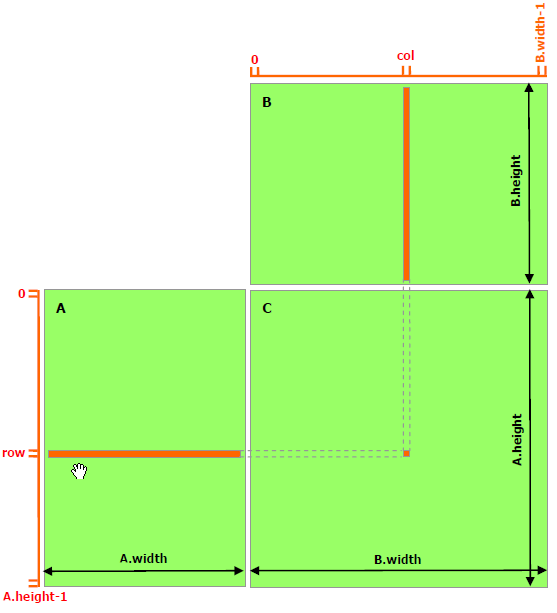
\includegraphics[width=\linewidth]{CUDA/matmul-wo-shared-memory.png}
  \caption{Global memory access pattern without shared memory in matrix multiplication}
\end{subfigure}%
\begin{subfigure}{.05\textwidth}
  \hspace{1cm}
\end{subfigure}%
\begin{subfigure}{.47\textwidth}
  \centering
  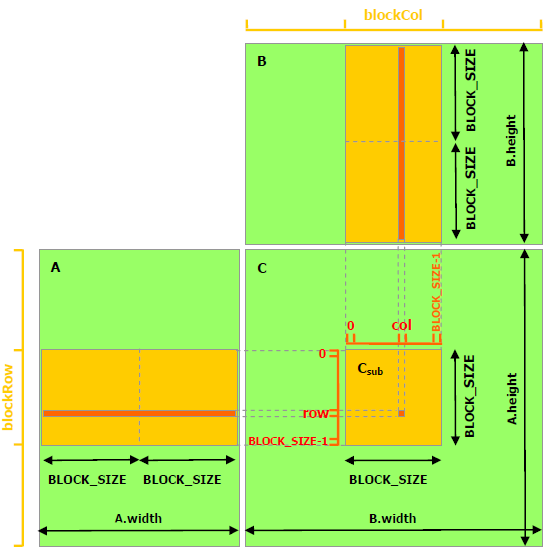
\includegraphics[width=\linewidth]{CUDA/matmul-w-shared-memory.png}
  \caption{Tiled matrix multiplication using shared memory for improved data reuse}
\end{subfigure}
\caption{Comparison of memory access strategies in matrix multiplication with and without shared memory in CUDA\footnote{3.2.4. Shared Memory: \url{https://docs.nvidia.com/cuda/cuda-c-programming-guide/index.html} (accessed April 16, 2025).}}
\label{fig:cuda-matmul-illustration}
\end{figure}

To further reduce memory access overhead—particularly evident in the synthetic XL dataset—shared memory is introduced as a performance optimization for matrix multiplication. Shared memory is an on-chip, low-latency memory region explicitly managed by the programmer within the CUDA programming model. In contrast to global memory, which resides off-chip and incurs higher access latency, shared memory enables efficient data reuse and thread-level communication within a thread block.

In this approach, threads within a block cooperatively load data from global memory into shared memory, perform intermediate computations using the cached values, and subsequently write the final results back to global memory. This strategy is especially effective for operations with repetitive data access patterns, such as matrix multiplication, where multiple threads require access to the same matrix elements.

Typically, in matrix multiplication, each thread computes a single output element by iterating over a row of the first matrix and a column of the second. Without shared memory, many threads redundantly fetch identical data from global memory, leading to inefficient access patterns and reduced performance. To mitigate this, a tiled matrix multiplication approach is adopted. In this method, the input matrices are divided into smaller sub-blocks (tiles), which are loaded into shared memory by each thread block. Once the tile data is available, threads within the block can reuse it across multiple computations before proceeding to the next tile. This technique significantly reduces the number of global memory transactions and enhances data locality.

However, the use of shared memory does not universally lead to performance gains. In the case of the MNIST dataset, which involves relatively small input sizes, the overhead of loading data into shared memory outweighs its benefits, resulting in a slight degradation in performance. For such lightweight computations, direct global memory access proves more efficient.

Therefore, in this implementation, shared memory optimization is selectively applied to the synthetic XL dataset, where the workload size justifies the additional overhead and facilitates improved throughput. A visual comparison of the memory access behavior in matrix multiplication with and without shared memory is provided in Figure~\ref{fig:cuda-matmul-illustration}, highlighting the reduction in redundant global memory accesses and the benefit of localized data reuse.
\subsection{Final Benchmarks}\label{subsec:cuda-final-benchmarks}
\begin{figure}[htb!]
\centering
\begin{subfigure}{.5\textwidth}
  \centering
  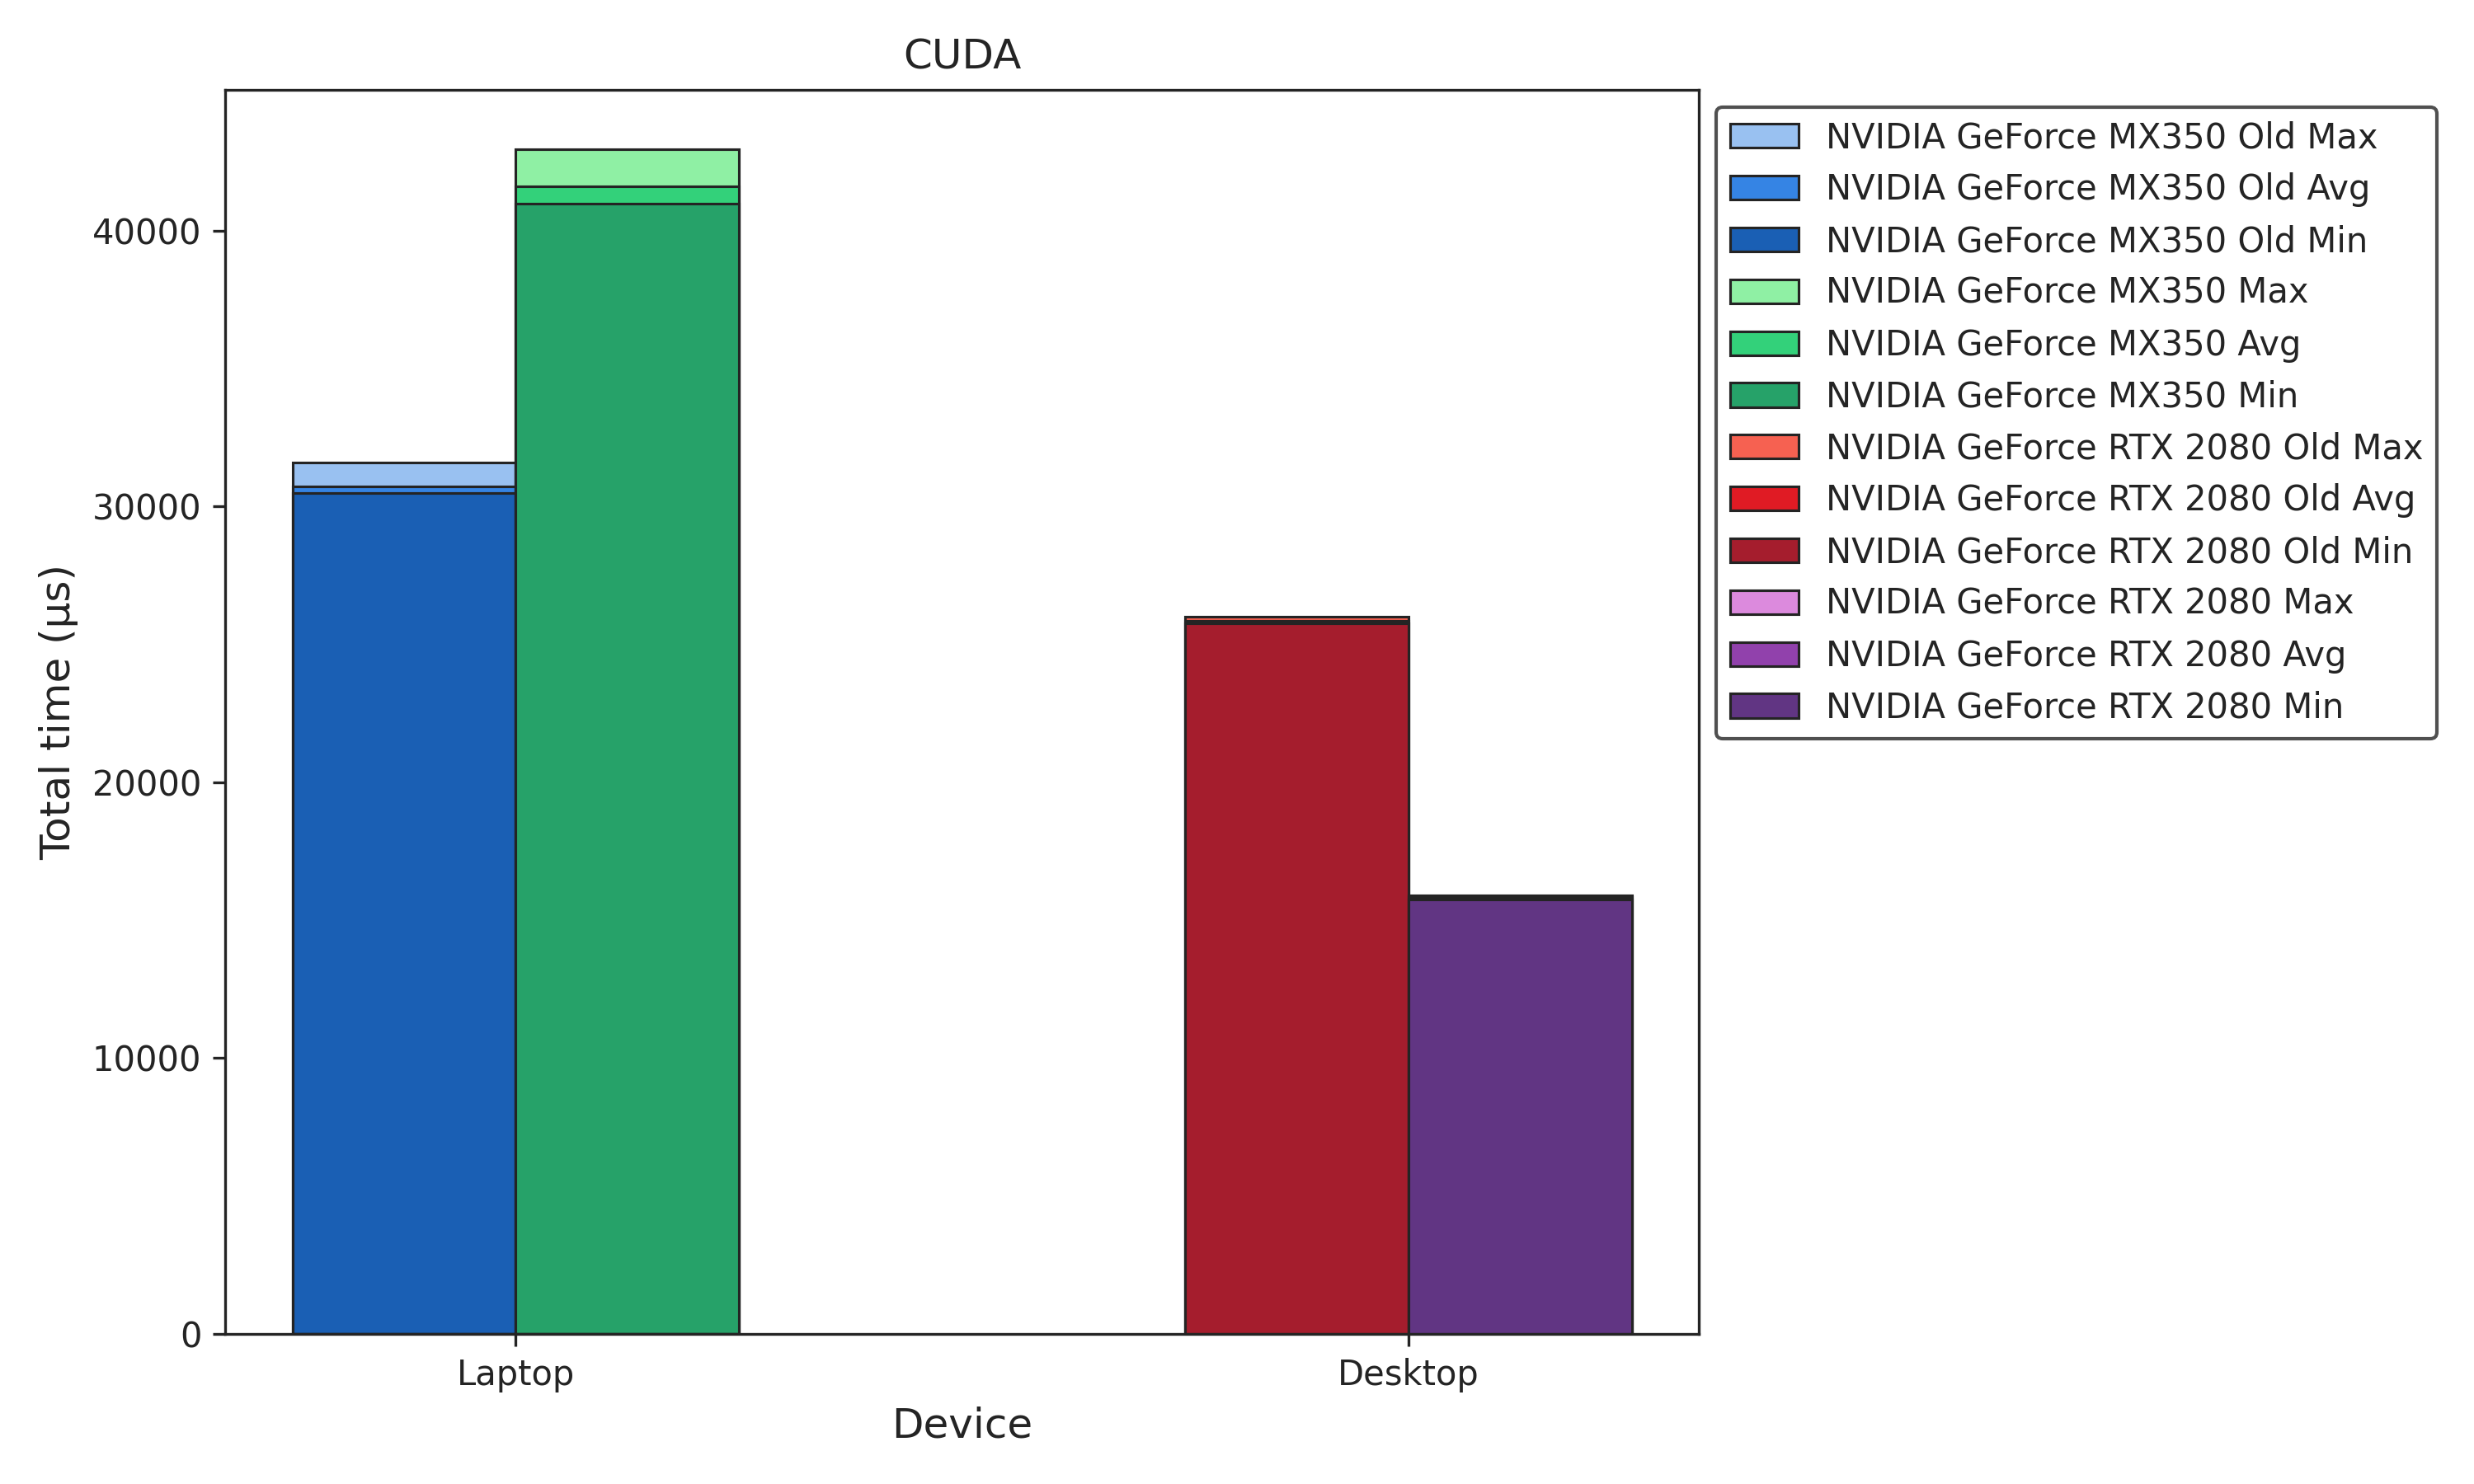
\includegraphics[width=\linewidth]{CUDA/CUDA_bugs_fixed.png}
  \caption{On the MNIST dataset}
\end{subfigure}%
\begin{subfigure}{.5\textwidth}
  \centering
  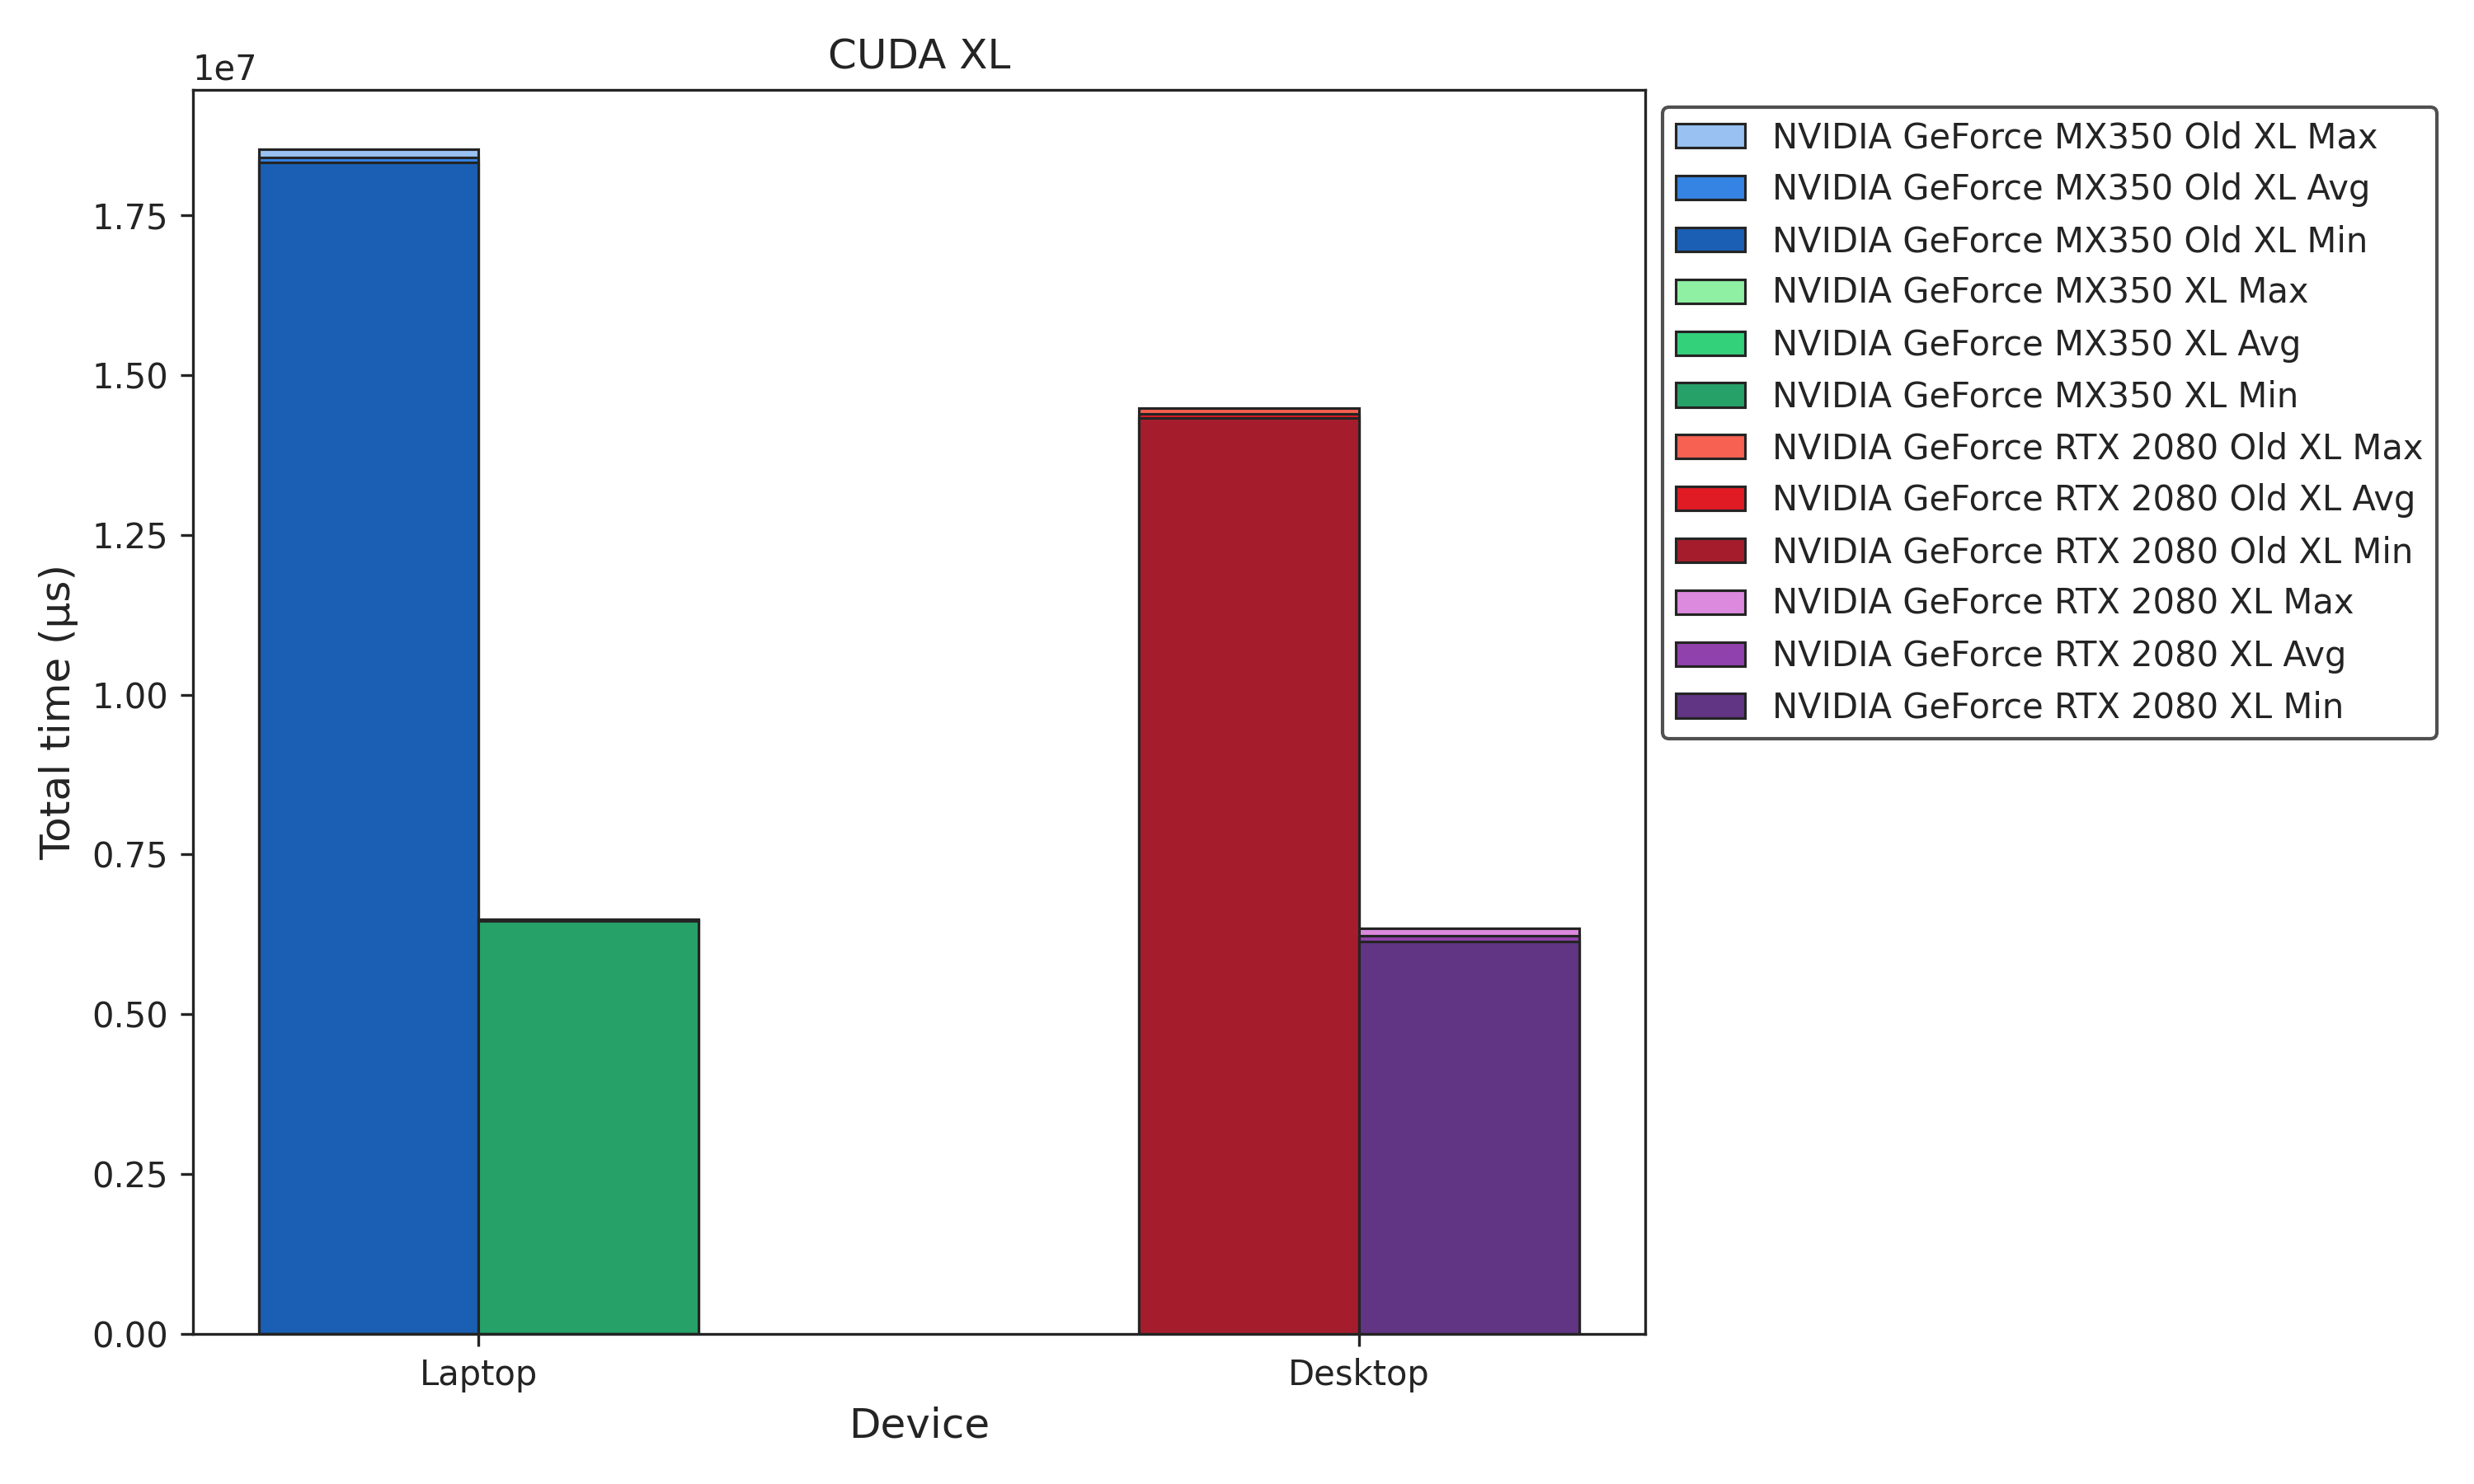
\includegraphics[width=\linewidth]{CUDA/CUDA XL_bugs_fixed.png}
  \caption{On the synthetic XL dataset}
\end{subfigure}
\caption{Performance benchmarks of the CUDA implementation, incorporating error resolution and shared memory optimization for matrix multiplication on the synthetic XL dataset}
\label{fig:cuda-final-bechmarks}
\end{figure}

\begin{table}[htb!]
\centering
\caption{CUDA Implementation\label{tab:cuda-final-benchmarks}}
\begin{tabular}{p{5.5cm} p{2cm} p{2cm} p{2cm} p{2cm}}
\hline
Benchmark Name & Minimum Value ($\mu$s) & Average Value ($\mu$s) & Maximum Value ($\mu$s) & Standard Deviation \\
\hline
NVIDIA GeForce MX350 \\
\hspace{0.5cm}Old & 30485.0 & 30713.7 & 31583.0 & 301.6 \\
\hspace{0.5cm}New & 40981.0 & 41606.3 & 42963.0 & 623.0 \\
NVIDIA GeForce RTX 2080 \\
\hspace{0.5cm}Old & 25756.0 & 25849.1 & 26018.0 & 78.6 \\
\hspace{0.5cm}New & 15742.0 & 15824.2 & 15910.0 & 55.7 \\
\hline
NVIDIA GeForce MX350 \\
\hspace{0.5cm}Old XL & 18332721.0 & 18399494.5 & 18536331.0 & 58421.0 \\
\hspace{0.5cm}New XL & 6456318.0 & 6471149.5 & 6486654.0 & 9872.8 \\
NVIDIA GeForce RTX 2080 \\
\hspace{0.5cm}Old XL & 14333244.0 & 14390205.3 & 14478414.0 & 47360.6 \\
\hspace{0.5cm}New XL & 6133257.0 & 6229544.3 & 6342743.0 & 78695.9 \\
\hline
\end{tabular}
\end{table}
\FloatBarrier

The final benchmark results, obtained after implementing the corrections outlined in Section~\ref{subsec:cuda-error-fixing} and the shared memory optimization discussed in Section~\ref{subsec:cuda-shared-memory}, are presented in Figure~\ref{fig:cuda-final-bechmarks}, with detailed values provided in Table~\ref{tab:cuda-final-benchmarks}. On the MNIST dataset, the average performance across both GPUs decreased by 1.5\%. This decline was driven by a 35.5\% performance reduction on the MX350, while the RTX 2080 exhibited a 38.8\% improvement. For the synthetic XL dataset, the average performance increased by 61.3\%, with gains of 64.8\% on the MX350 and 56.7\% on the RTX 2080.

The MNIST benchmark yielded mixed results. The RTX 2080 demonstrated a substantial improvement, consistent with the preceding optimization stages. In contrast, the MX350 experienced a significant performance drop. One plausible explanation is thermal throttling, as extended benchmarking sessions—reaching up to six hours—likely caused the laptop to overheat. Given that the MX350 operates within a mobile platform with limited thermal dissipation capabilities, sustained high-intensity workloads may have triggered reduced operating frequencies, thereby impacting performance.

For the synthetic XL dataset, both GPUs showed considerable improvements relative to the baseline. Execution time was reduced by over 60\%, illustrating the cumulative impact of the applied optimizations. Interestingly, the performance of the MX350 and RTX 2080 converged for this workload, despite substantial hardware differences. This convergence suggests that the XL dataset, while larger than MNIST, remains insufficient to fully utilize the computational capacity of the RTX 2080.


Despite the applied optimizations aimed at minimizing memory transfer overhead, these operations still account for more than 32.4\% of the total execution time. This reinforces the observation that a substantial portion of GPU computation time is often spent on memory-related tasks, highlighting memory management as a critical factor in overall performance.

These findings highlight a key characteristic of GPU performance: scalability with problem size. For more demanding tasks—such as training deep neural networks or large language models—the performance gap between high-end and low-power GPUs would be expected to widen significantly, better reflecting the architectural advantages of higher-tier hardware.
\subsection{Inital vs. Final Benchmarks}
\begin{figure}[htb!]
\centering
\begin{subfigure}{.5\textwidth}
  \centering
  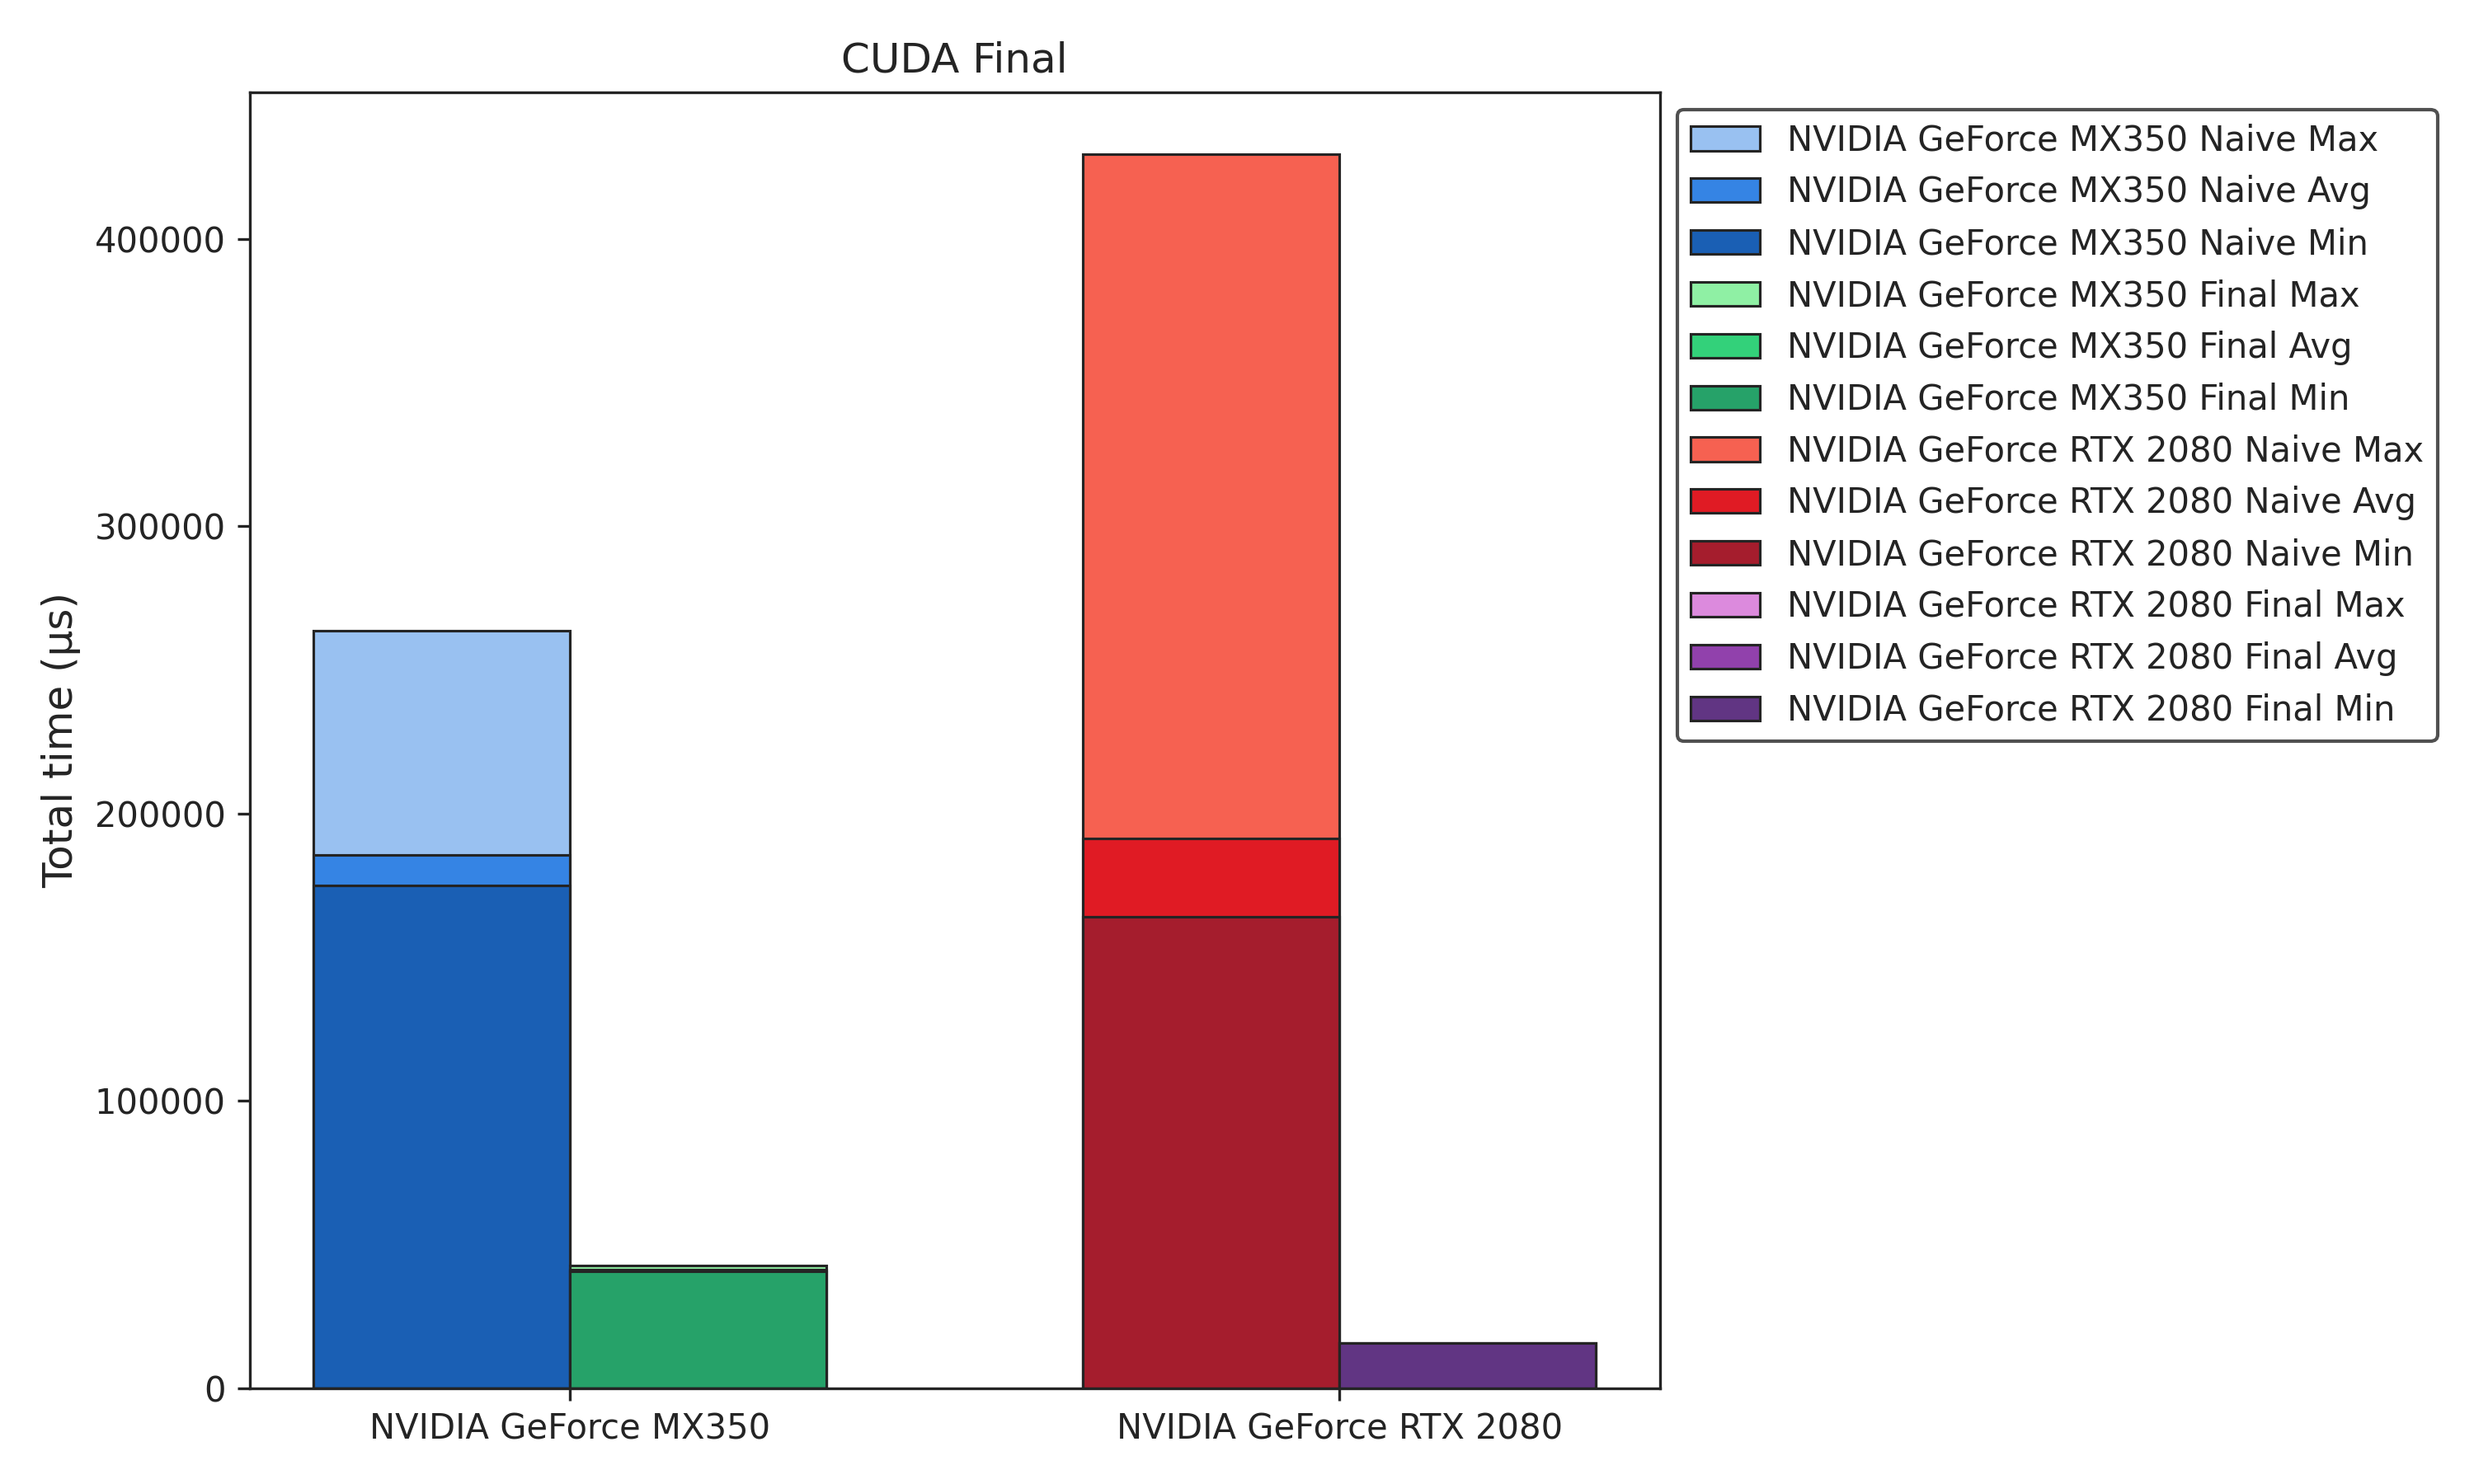
\includegraphics[width=\linewidth]{CUDA/CUDA_initial_vs_final.png}
  \caption{On the MNIST dataset}
\end{subfigure}%
\begin{subfigure}{.5\textwidth}
  \centering
  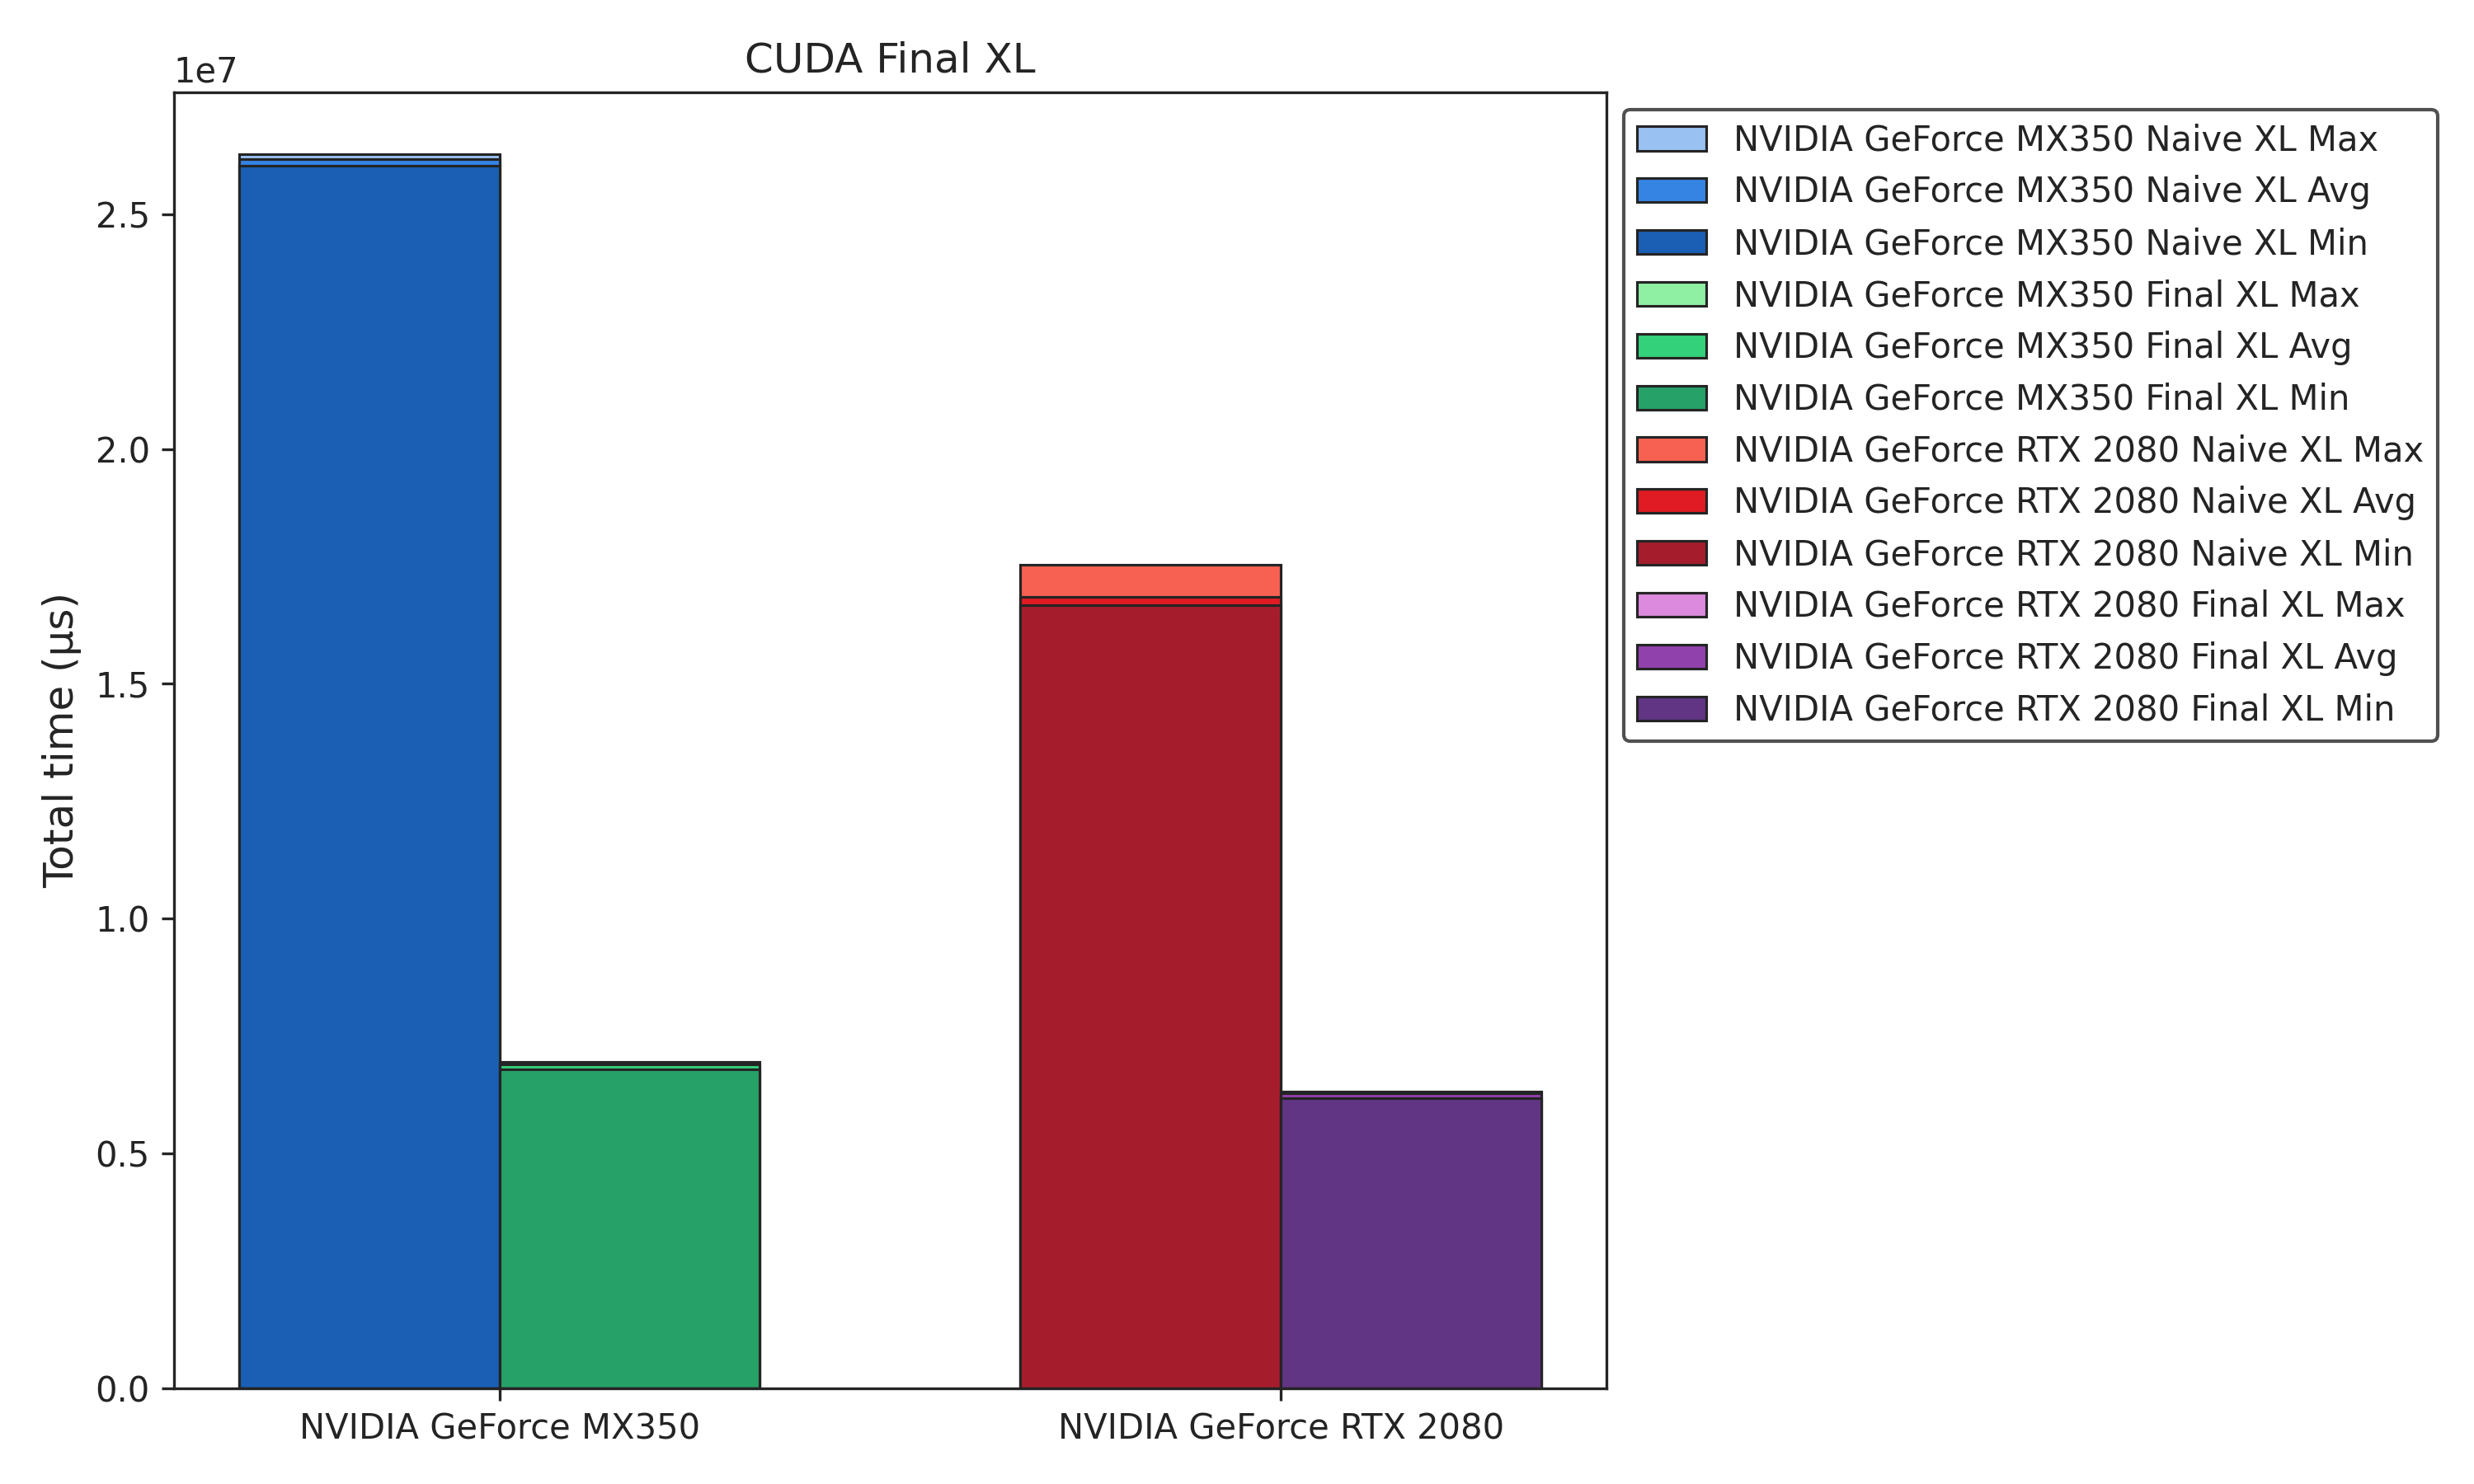
\includegraphics[width=\linewidth]{CUDA/CUDA XL_initial_vs_final.png}
  \caption{On the synthetic XL dataset}
\end{subfigure}
\caption{Evaluation of performance improvements between baseline and final implementation}
\label{fig:cuda-initial-vs-final-bechmarks}
\end{figure}

\begin{table}[htb!]
\centering
\caption{CUDA Implementation\label{tab:cuda-initial-vs-final-benchmarks}}
\begin{tabular}{p{5.5cm} p{2cm} p{2cm} p{2cm} p{2cm}}
\hline
Benchmark Name & Minimum Value ($\mu$s) & Average Value ($\mu$s) & Maximum Value ($\mu$s) & Standard Deviation \\
\hline
NVIDIA GeForce MX350 \\
\hspace{0.5cm}Naive & 174935.0 & 185643.7 & 263690.0 & 26088.6 \\
\hspace{0.5cm}Final & 40666.0 & 41263.0 & 42664.0 & 602.2 \\
NVIDIA GeForce RTX 2080 \\
\hspace{0.5cm}Naive & 163977.0 & 191287.6 & 429508.0 & 79409.7 \\
\hspace{0.5cm}Final & 15692.0 & 15737.8 & 15769.0 & 24.0 \\
\hline
NVIDIA GeForce MX350 \\
\hspace{0.5cm}Naive XL & 26024991.0 & 26167448.5 & 26279652.0 & 87379.6 \\
\hspace{0.5cm}Final XL & 6793943.0 & 6896478.6 & 6941920.0 & 43924.6 \\
NVIDIA GeForce RTX 2080 \\
\hspace{0.5cm}Naive XL & 16678725.0 & 16850845.9 & 17539716.0 & 242817.9 \\
\hspace{0.5cm}Final XL & 6179128.0 & 6274309.0 & 6311310.0 & 35139.3 \\
\hline
\end{tabular}
\end{table}
\FloatBarrier

A summary of the overall performance improvements achieved throughout the optimization process is presented in Figure~\ref{fig:cuda-initial-vs-final-bechmarks}, with detailed values listed in Table~\ref{tab:cuda-initial-vs-final-benchmarks}. On the MNIST dataset, average performance across both GPUs improved by 84.9\%, with gains of 77.8\% on the MX350 and 91.8\% on the RTX 2080. For the synthetic XL dataset, the average speedup was 69.4\%, comprising a 73.6\% improvement on the MX350 and a 62.8\% improvement on the RTX 2080.

The project began with a naive CUDA implementation that made limited use of available GPU resources. The initial version exhibited suboptimal thread utilization, redundant memory transfers between host and device, and no use of specialized memory types. Throughout the project, a sequence of targeted optimizations was applied to address these limitations.

These optimizations included maximizing thread occupancy, eliminating unnecessary data movement, correcting implementation-level inefficiencies, and strategically integrating constant and shared memory in areas where data reuse was significant. Each of these changes was intended to better align the implementation with the execution model and architectural features of modern GPUs.

The final benchmarks confirm the cumulative effectiveness of these optimizations. As shown in Figure~\ref{fig:cuda-initial-vs-final-bechmarks}, both datasets benefited significantly from the improved resource management and execution strategy. This result underscores the importance of systematic optimization in GPU-accelerated applications and demonstrates the performance gains that can be achieved through deliberate hardware-aware programming practices.
\section{CPU vs. GPU}\label{sec:cpu-vs-gpu}
\begin{figure}[htb!]
    \centering
    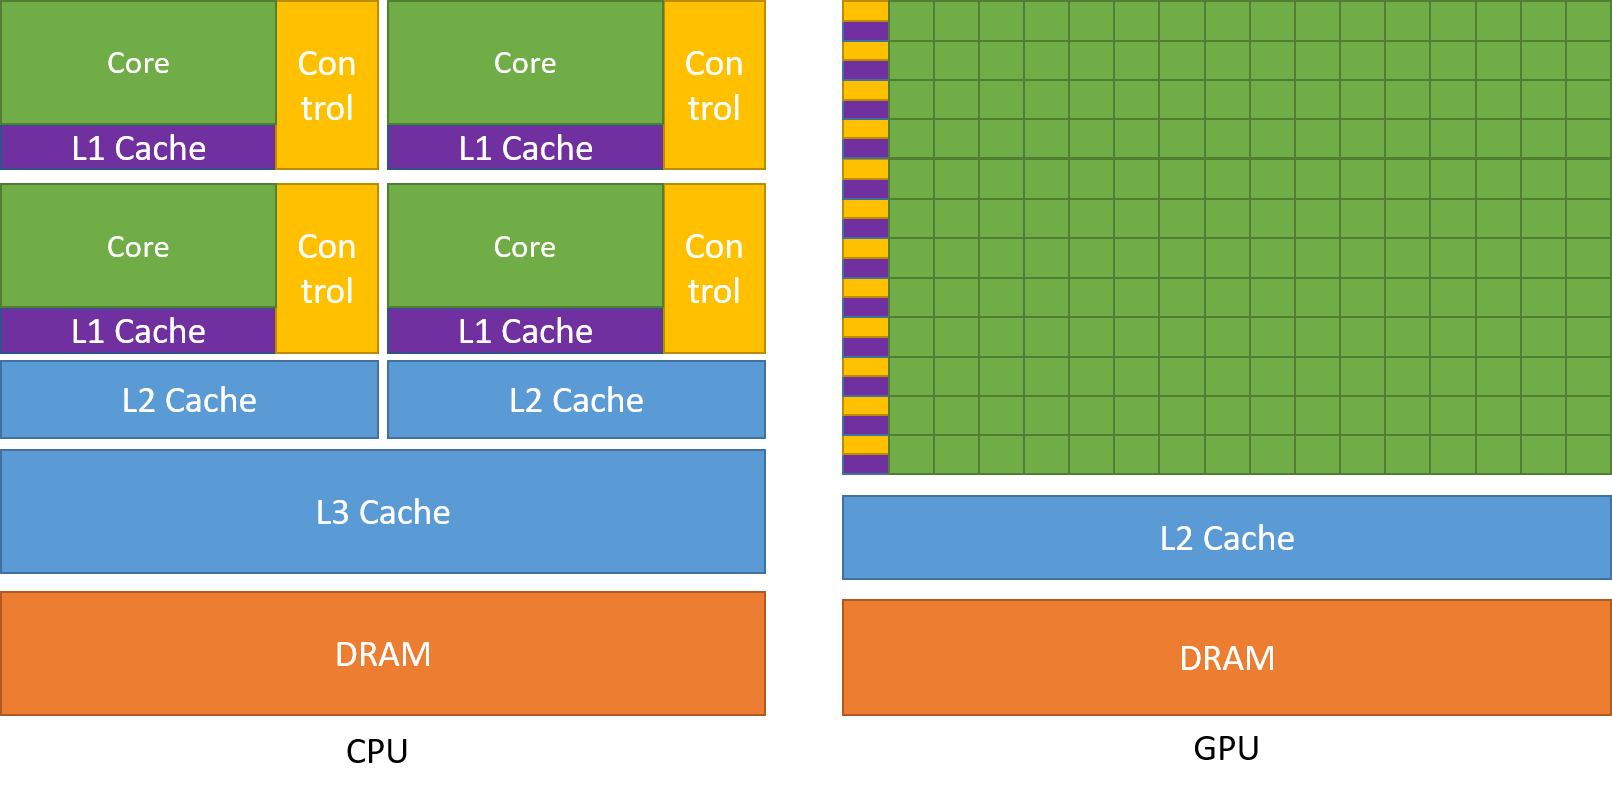
\includegraphics[width=0.8\linewidth]{CUDA/gpu-vs-cpu-transistors.png}
    \caption{Comparison of the number of transistors dedicated to specific tasks in GPU and CPU architectures\footnote{1.1. The Benefits of Using GPUs: \url{https://docs.nvidia.com/cuda/cuda-c-programming-guide/index.html} (accessed April 16, 2025).}}
   \label{fig:cpu-vs-gpu-transistors}
\end{figure}

Before analyzing the optimizations implemented in this work, it is important to understand the fundamental architectural differences between CPUs and GPUs, and why the latter are preferred for highly parallel workloads. As illustrated in Figure~\ref{fig:cpu-vs-gpu-transistors}, the GPU architecture dedicates the majority of its transistors to arithmetic and logic units, maximizing raw computational throughput. In contrast, CPUs exhibit a more complex and control-heavy design, with a significant portion of the transistor budget allocated to control logic and large multi-level cache hierarchies.

CPUs are optimized for low-latency, sequential processing and are highly effective in scenarios requiring frequent branching, task switching, or tight synchronization. Their sophisticated caching systems help mitigate memory latency by keeping frequently accessed data close to the processing units.

GPUs, by comparison, minimize control complexity and cache size in favor of massive parallelism. Rather than hiding memory latency through caching, GPUs overcome it by executing thousands of threads concurrently, thereby maintaining high utilization even in the presence of memory stalls. This makes them particularly well suited for data-parallel workloads, such as those found in scientific computing, graphics rendering, and modern machine learning applications.

These characteristics explain the increasing prevalence of GPU-accelerated datacenters and their central role in the current era of AI and deep learning, where large-scale neural networks benefit significantly from the GPU’s parallel processing capabilities.
\subsection{Performance Benchmarks}
\begin{figure}[htb!]
\centering
\begin{subfigure}{.5\textwidth}
  \centering
  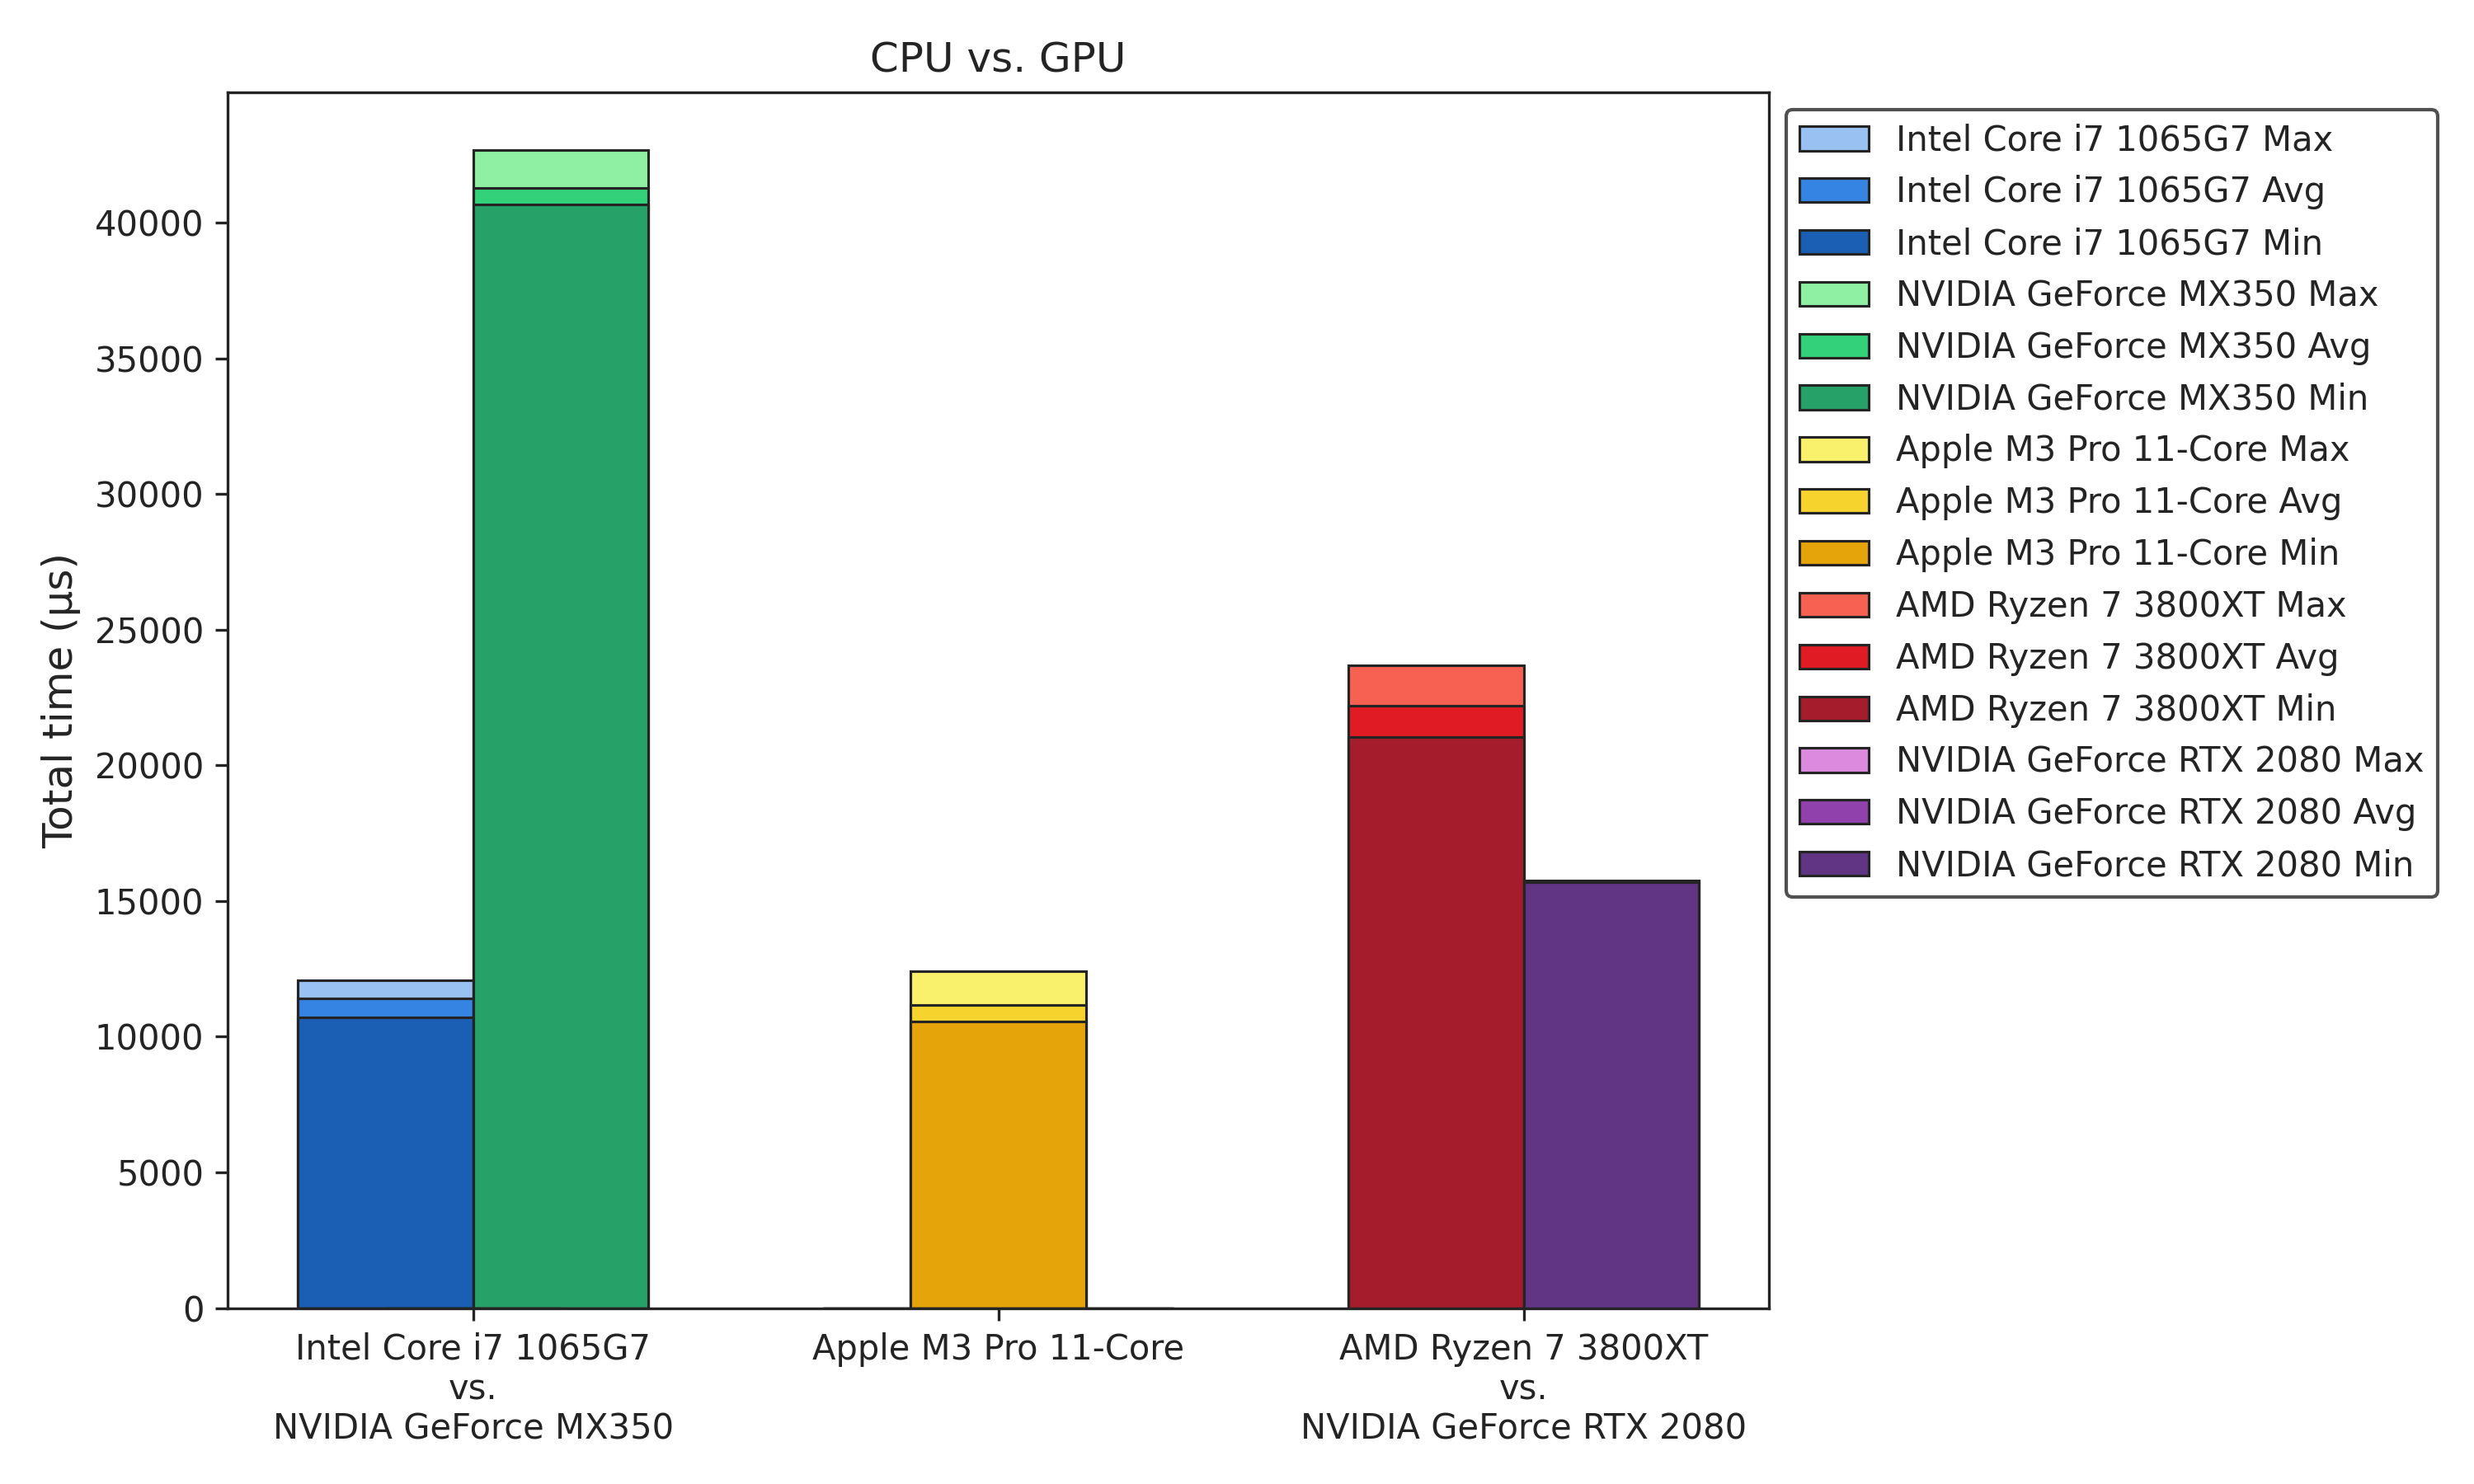
\includegraphics[width=\linewidth]{Graphs/CPU vs. GPU.png}
  \caption{On the MNIST dataset}
\end{subfigure}%
\begin{subfigure}{.5\textwidth}
  \centering
  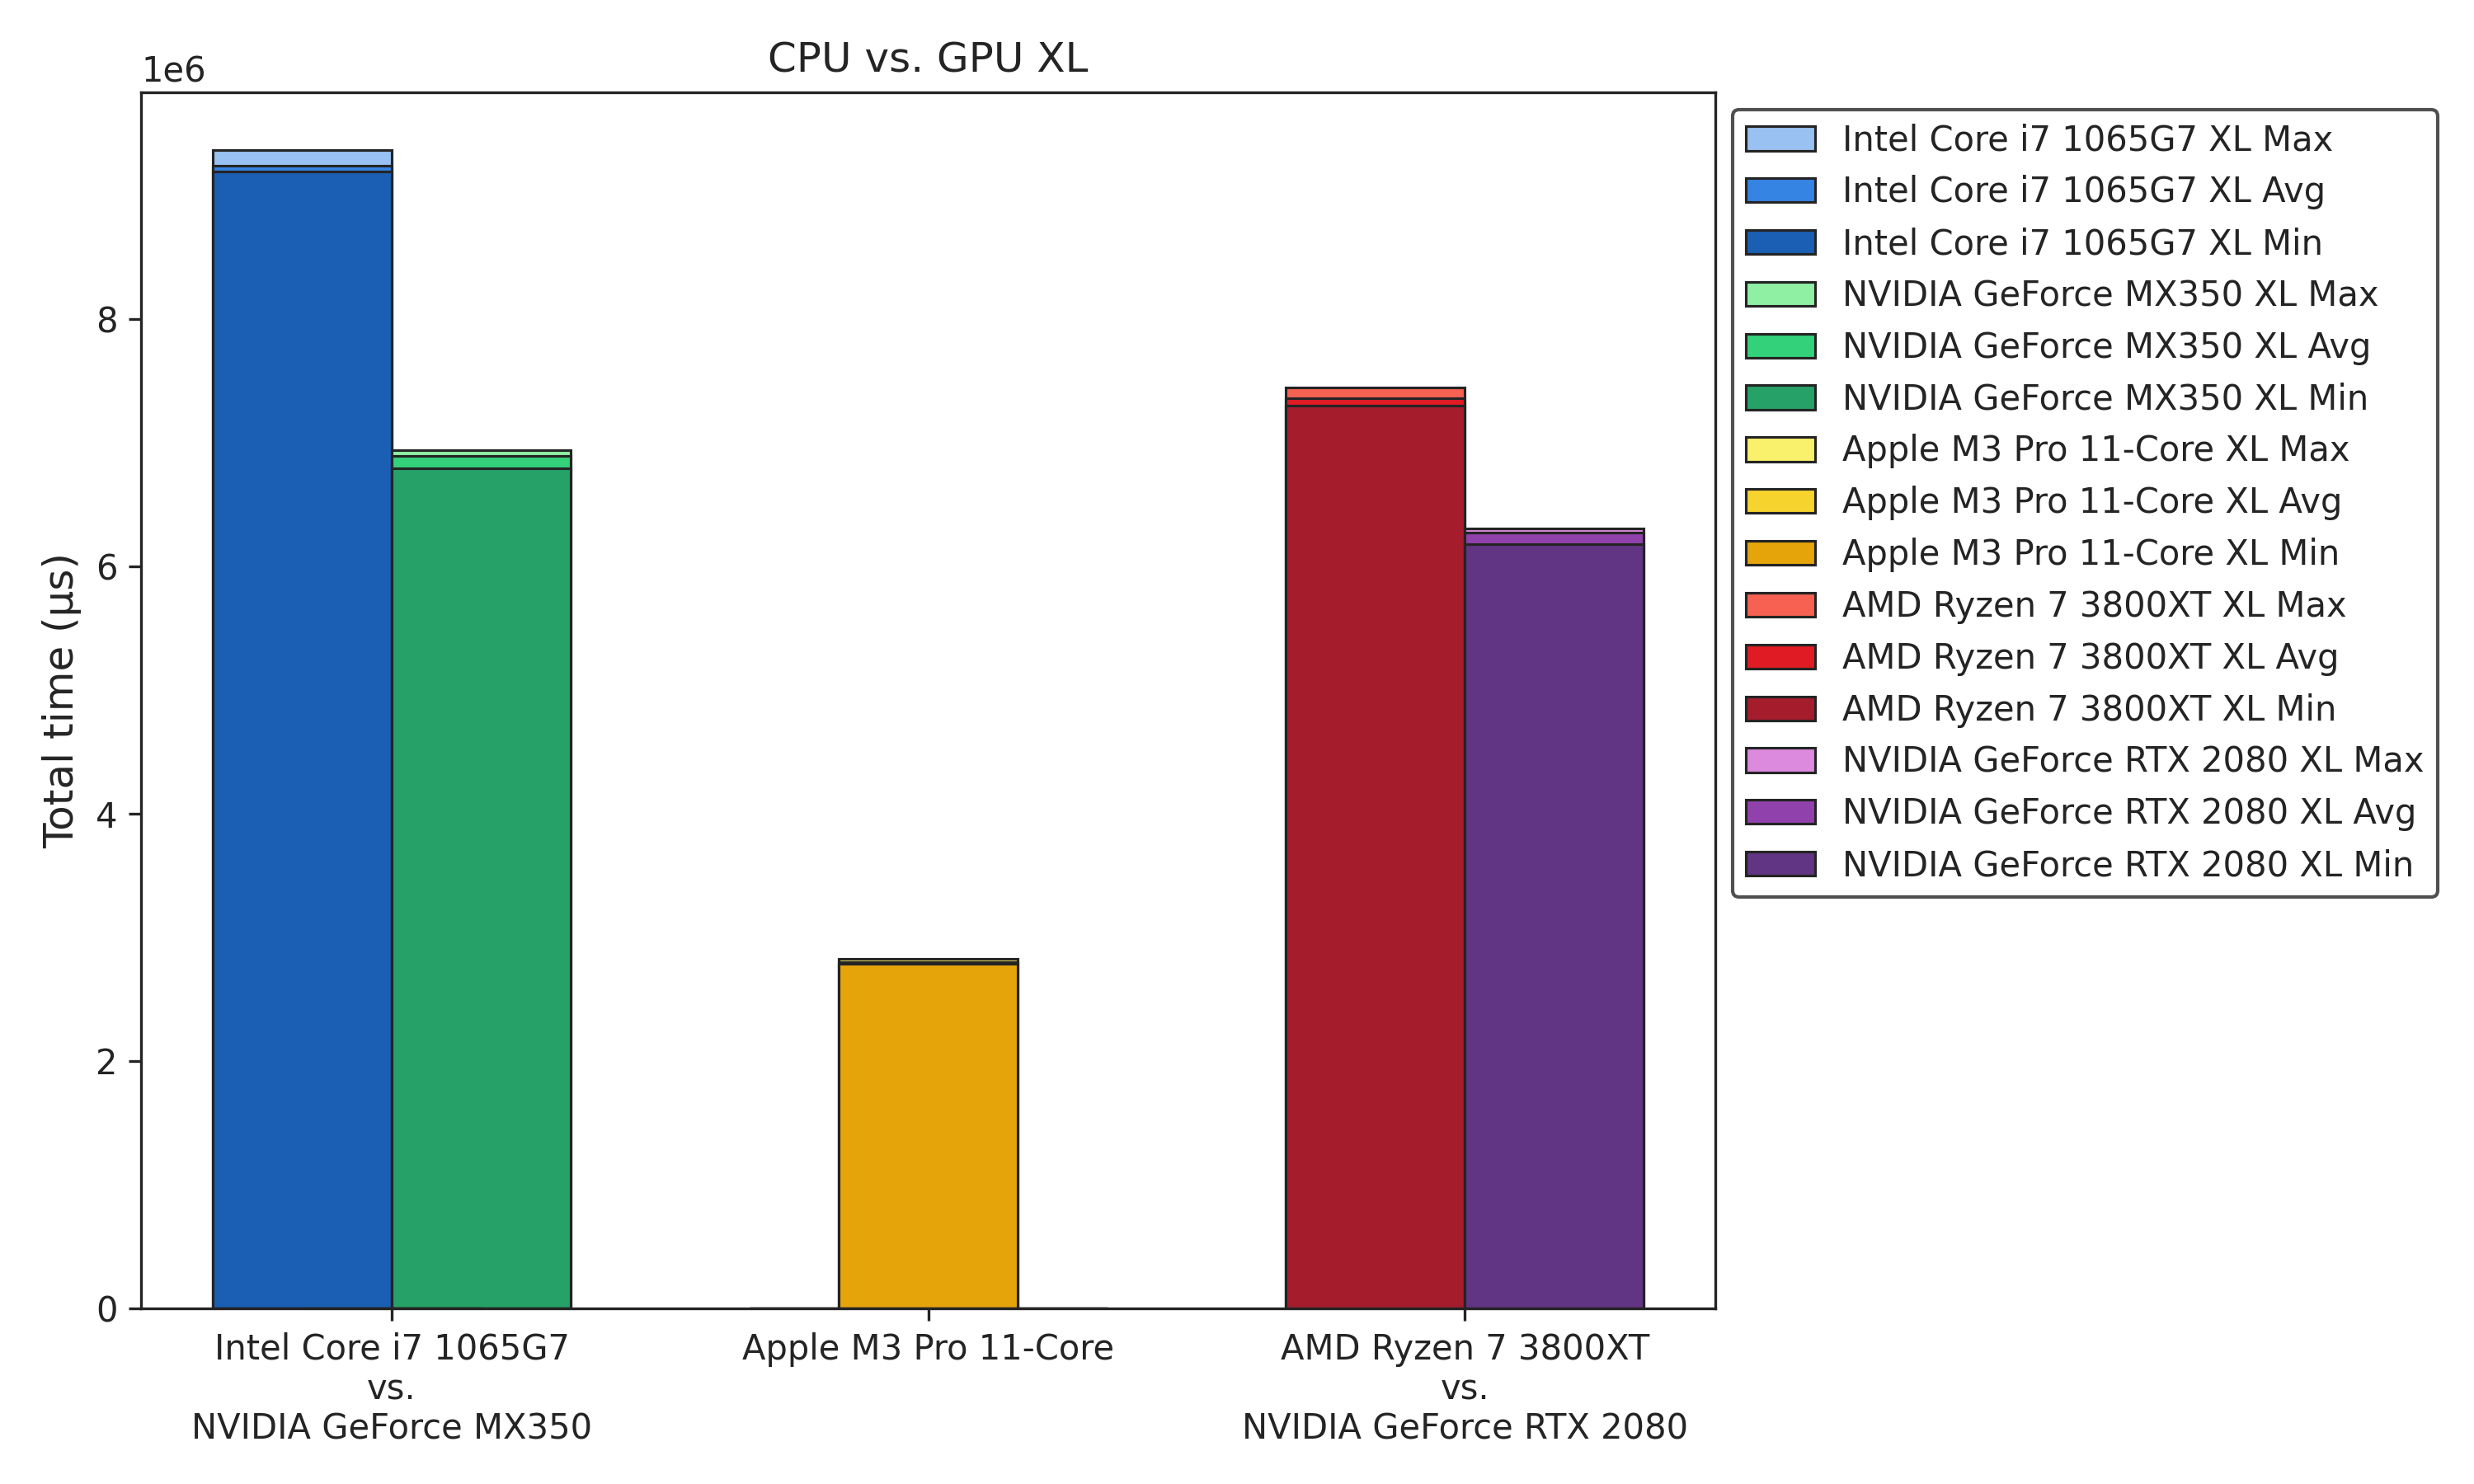
\includegraphics[width=\linewidth]{Graphs/CPU vs. GPU XL.png}
  \caption{On the synthetic XL dataset}
\end{subfigure}
\caption{Comparison of execution performance between fully optimized CPU and GPU implementations}
\label{fig:cpu-vs-gpu-benchmarks}
\end{figure}

\begin{table}[htb!]
\centering
\caption{CUDA Implementation vs. CPU Implementation\label{tab:cpu-vs-gpu-benchmarks}}
\begin{tabular}{p{5.5cm} p{2cm} p{2cm} p{2cm} p{2cm}}
\hline
Benchmark Name & Minimum Value ($\mu$s) & Average Value ($\mu$s) & Maximum Value ($\mu$s) & Standard Deviation \\
\hline
Intel Core i7-1065G7 & 10725.0 & 11398.8 & 12087.0 & 417.5 \\
NVIDIA GeForce MX350 & 40666.0 & 41263.0 & 42664.0 & 602.2 \\
Apple M3 Pro 11-Core & 10575.0 & 11170.5 & 12407.0 & 618.4 \\
AMD Ryzen 7 3800XT & 21050.0 & 22202.5 & 23671.0 & 747.3 \\
NVIDIA GeForce RTX 2080 & 15692.0 & 15737.8 & 15769.0 & 24.0 \\
\hline
Intel Core i7-1065G7 XL & 9195229.0 & 9246640.6 & 9369463.0 & 52836.7 \\
NVIDIA GeForce MX350 XL & 6793943.0 & 6896478.6 & 6941920.0 & 43924.6 \\
Apple M3 Pro 11-Core XL & 2783871.0 & 2802165.9 & 2824752.0 & 13541.5 \\
AMD Ryzen 7 3800XT XL & 7302691.0 & 7361732.2 & 7450227.0 & 50234.5 \\
NVIDIA GeForce RTX 2080 XL & 6179128.0 & 6274309.0 & 6311310.0 & 35139.3 \\
\hline
\end{tabular}
\end{table}
\FloatBarrier

The benchmark results are shown in Figure~\ref{fig:cpu-vs-gpu-benchmarks}, with the corresponding values listed in Table~\ref{tab:cpu-vs-gpu-benchmarks}. On average, the GPUs perform 52.3\% worse than their corresponding CPUs on the MNIST dataset. The NVIDIA GeForce MX350 is 262.0\% slower than the Intel Core i7-1065G7, while the NVIDIA GeForce RTX 2080 is 29.1\% faster than the AMD Ryzen 7 3800XT. Meanwhile, the Apple M3 Pro 11-Core is on average 60.8\% faster than the GPU implementations. On the synthtetic XL dataset the GPU is on average 17.7\% faster than their corresponding CPUs. The NVIDIA GeForce MX350 is on average 25.4\% faster than the Intel Core i7-1065G7. The NVIDIA GeForce RTX 2080 is on average 14.8\% faster than the AMD Ryzen 7 3800XT. Still, the Apple M3 Pro 11-Core is on average 57.4\% faster than the GPU implementations.
\section{Conclusion}\label{sec:conclusion}
To ensure reproducibility and fair comparison, a dedicated benchmarking framework was developed. It enabled controlled testing across a diverse set of CPU and GPU architectures, facilitating consistent evaluation across varying workload sizes.

OpenMP was evaluated as a high-level parallelization solution but proved unsuitable for performance-critical inference workloads.

Development initially began using GCC but transitioned to Clang due to compatibility requirements on Apple Silicon. Although Intel’s ICPX compiler showed stronger optimization potential, it was not available across all platforms, requiring a consistent toolchain.

CPU optimizations proceeded in several phases. The initial multithreading approach introduced overhead, which was mitigated through the introduction of a thread pool and dynamic parallelism based on input size. Instruction-level parallelism was then introduced using SIMD extensions, including SSE, AVX, AVX2, and AVX-512, to accelerate element-wise operations. Compiler vectorization and memory-aligned data structures further enhanced throughput. Emerging technologies like AMX were also considered as promising future directions. Cache-aware blocking and generalized threading logic completed the optimization pipeline.

GPU improvements followed a structured process. First, thread configurations were tuned to improve occupancy. Redundant memory copies between host and device were then minimized, and constant memory was used to accelerate access to static inference weights. Further overhead was removed by eliminating unnecessary transfers, resolving functional errors, and finally introducing shared memory for tiled matrix operations. These optimizations substantially reduced latency and improved utilization of GPU memory hierarchies.

A direct comparison between CPU and GPU performance revealed that computational efficiency is strongly influenced by problem size. For smaller workloads, CPUs exhibited superior performance due to lower overhead and more effective cache utilization. However, as input size increased, GPUs began to outperform CPUs by leveraging their extensive parallelism and higher memory bandwidth. Interestingly, even though the CPU implementation utilized multithreading at the image level—while the GPU implementation did not parallelize across images—the GPU still outperformed the CPU on the synthetic XL dataset. This result highlights the scalability advantages of GPU architectures for large-scale data processing. The identified crossover point in performance illustrates that neither architecture is universally optimal. While CPUs remain well-suited for small, latency-sensitive workloads, GPUs are likely to outperform CPUs once a certain workload size is exceeded—particularly in tasks such as matrix operations or neural network inference, where parallelism can be fully exploited.

Apple Silicon stood out in our benchmarks, consistently outperforming older x86 CPUs and GPUs. This advantage stems from its newer architecture, efficient memory design, and integrated processing. However, it is likely that modern high-end GPUs such as the NVIDIA RTX 4090 would surpass its performance in large-scale scenarios.

The proposed framework offers a modular, extensible, and architecture-aware basis for future research on performance optimization. As AI workloads continue to evolve, such tools are essential for enabling informed decisions in real-world deployments.
\section{List of Figures, Listings, and Tables}
\def\lofname{Figures}
\listoffigures
\def\tocname{Listings}
\lstlistoflistings
\def\lotname{Tables}
\listoftables
\section{References}
\renewcommand{\notesname}{Sources}
\theendnotes
\section{Responsibilities}
Maximilian Achenbach authored the following chapters:
\begin{enumerate}
    \item Chapter~\ref{sec:gpu-based-optimizations}: GPU-Based Optimizations
    \item Chapter~\ref{sec:cpu-vs-gpu}: CPU vs. GPU
    \item Chapter~\ref{sec:conclusion}: Conclusion
\end{enumerate}
Dustin Heither authored the following chapters and sections:
\begin{enumerate}
    \item Chapter~\ref{sec:openmp}: OpenMP
    \item Section~\ref{subsec:gcc-and-clang}: GCC and Clang
    \item Section~\ref{subsec:overview-of-simd}: Overview of SIMD
    \item Section~\ref{subsec:arm-optimizations}: Arm Optimizations
    \item Chapter~\ref{sec:quantization}: Quantization
\end{enumerate}
Robert Kagan authored the following chapters and sections:
\begin{enumerate}
    \item Chapter~\ref{sec:multithreading}: Multithreading
    \item Section~\ref{subsec:intel-c++-compiler}: Intel C++ Compiler
    \item Section~\ref{subsec:dialog}: Dialog
    \item Section~\ref{subsec:x86-optimizations}: x86 Optimizations
    \item Chapter~\ref{sec:other-optimizations}: Other Optimizations
    \item Chapter~\ref{sec:inital-vs-final-implementation}: Inital vs. Final Implementation
\end{enumerate}
Collaboratively authored were the following chapters:
\begin{enumerate}
    \item Abstract
    \item Chapter~\ref{sec:introduction}: Introduction 
    \item Chapter~\ref{sec:objective}: Objective
    \item Chapter~\ref{sec:benchmarking-setup}: Benchmarking Setup
    \item Chapter~\ref{sec:naive-implementation}: Naive Implementation
\end{enumerate}
\end{document}
% End of file `Optimizing_AI_Workloads_for_Enhanced_Performance__A_Comprehensive_Framework_for_Comparing_CPU_and_GPU_Architectures.tex'.
